\documentclass[11pt]{article}
\usepackage[a4paper,margin=27mm]{geometry}
\usepackage{amsmath,amssymb,amsthm}
\usepackage{bm}
\usepackage{graphicx}
\usepackage{booktabs}
\usepackage{tabularx}

% The former tcolorbox comment environment was unused and has been removed.
\newcolumntype{Y}{>{\raggedright\arraybackslash}X}
\usepackage{tikz}
\usetikzlibrary{arrows.meta,positioning}
% Compact author--year abbreviations are supplied by the optional
% \bibitem labels in the bibliography.
\usepackage[
  colorlinks=true,
  linkcolor=black,
  citecolor=black,
  urlcolor=black,
  pdftitle={Partial Stabilizer Learning under Fixed Commuting Constraints and the Absence of a Copy-Rate Discount},
  pdfauthor={Masahito Hayashi and Yimin Lu},
  pdfsubject={Partial stabilizer learning under fixed commuting constraints},
  pdfkeywords={stabilizer learning, quantum state identification, verification, Clifford covariance, sample complexity}
]{hyperref}
\allowdisplaybreaks
\setlength{\emergencystretch}{2em}

% Common notation and theorem environments.
\newcommand{\F}{\mathbb F}
\newcommand{\Z}{\mathbb Z}
\newcommand{\Sym}{\operatorname{Sym}}
\newcommand{\rank}{\operatorname{rank}}
\newcommand{\im}{\operatorname{Im}}
\newcommand{\diag}{\operatorname{diag}}
\newcommand{\Tr}{\operatorname{Tr}}
\newcommand{\odotv}{\mathbin{\odot}}
\newcommand{\1}{\mathbf 1}
\newcommand{\E}{\mathbb E}
\newcommand{\supp}{\operatorname{supp}}
\newcommand{\PGM}{\mathrm{PGM}}
\newcommand{\spair}[2]{\langle #1,#2\rangle_{\mathrm{sp}}}

\newcommand{\ket}[1]{\lvert #1\rangle}
\newcommand{\bra}[1]{\langle #1\rvert}
\newcommand{\braket}[2]{\langle #1\mid #2\rangle}

\theoremstyle{plain}
\newtheorem{theorem}{Theorem}[section]
\newtheorem{lemma}[theorem]{Lemma}
\newtheorem{proposition}[theorem]{Proposition}
\newtheorem{corollary}[theorem]{Corollary}
\theoremstyle{definition}
\newtheorem{definition}[theorem]{Definition}
\theoremstyle{remark}
\newtheorem{remark}[theorem]{Remark}

\title{Partial Stabilizer Learning under Fixed Commuting Constraints and the Absence of a Copy-Rate Discount}
\author{%
\parbox{0.95\textwidth}{\centering
Masahito Hayashi\textsuperscript{1,2,3}
\quad
Yimin Lu\textsuperscript{4}\\[0.75em]
\small
\textsuperscript{1}School of Data Science, The Chinese University of Hong Kong,
Shenzhen, Longgang District, Shenzhen 518172 Guangdong, China.\\
\textsuperscript{2}International Quantum Academy, Futian District,
Shenzhen 518048 Guangdong, China.\\
\textsuperscript{3}Graduate School of Mathematics, Nagoya University,
Chikusa-ku, Nagoya 464--8602 Aichi, Japan.\\
\textsuperscript{4}Yau Mathematical Sciences Center, Tsinghua University,
Beijing 100084, China.}}
\date{}

\begin{document}
\maketitle

\begin{abstract}
We consider an unknown pure stabilizer state of \(n\) qudits with a fixed prime local dimension \(p\), together with prescribed commuting Pauli observables. Rather than learning the whole state, the learner must recover only complementary stabilizers that commute with the prescribed observables, together with their eigenvalues. Once the prescribed measurement is performed, this information and the observed outcome determine the corresponding conditional stabilizer state. We compare the number \(k\) of copies available to the learner with the number \(n\) of qudits and refer to their ratio \(k/n\) as the copy rate.
Suppose that the dimension \(m\) of the requested complementary stabilizer subspace satisfies \(m=\beta n+o(n)\) for a fixed \(0<\beta\leq1\). If the copy rate converges to a value below one, the optimal exact recovery probabilities and verification scores converge to zero, both in the worst case and under the uniform prior. Conversely, if the number \(k\) of copies minus the number \(n\) of qudits tends to positive infinity, the entire stabilizer state can be identified with probability tending to one, and the requested complementary information can then be extracted. Thus, restricting the learning target to the stabilizer information needed after the prescribed measurement yields no copy-rate discount.
\end{abstract}
\section{Introduction}
\label{sec:introduction}
Many quantum-information tasks require only selected classical information about an unknown state rather than a complete state description. 
Examples include estimating the acceptance probabilities of prescribed measurements~\cite{Aaronson2018ShadowTomography, BadescuODonnell2024ImprovedQuantumData, KingEtAl2025TriplyEfficient, Sinha2025DimensionIndependent}, 
constructing reusable classical representations for predicting selected state properties~\cite{HuangKuengPreskill2020ClassicalShadows, ChenYuZengFlammia2021RobustShadows, HadfieldEtAl2022LocallyBiasedShadows, BertoniEtAl2024ShallowShadows}, 
and reconstructing reduced density matrices on specified subsystems~\cite{CotlerWilczek2020OverlappingTomography, BonetMonroigBabbushOBrien2020PartialTomography, AraujoEtAl2022LocalOverlappingTomography, HansenneEtAl2025OptimalOverlapping}. 
In their respective settings, these results show that task-specific characterization can require substantially fewer quantum samples or measurement settings than full tomography. 
We ask whether requiring only selected information about a structured quantum state, rather than its complete description, can likewise reduce the leading-order quantum copy complexity.


We study an unknown pure stabilizer state of $n$ qudits with arbitrary prime local dimension $p$, together with prescribed commuting Pauli observables.   
The learner receives copies of the initial state and knows the prescribed measurement, but must produce its report before the measurement outcome is observed. Once an outcome has been obtained, the report and that outcome should identify the corresponding conditional stabilizer state.
To meet this requirement, the learner need not identify the entire initial state, but only the part of its stabilizer description that commutes with the prescribed observables, together with the corresponding eigenvalues. 
Pauli directions are represented by the symplectic vector space $\F_p^{2n}$. 
Two Pauli directions commute exactly when their symplectic inner product vanishes. 
A subspace on which this inner product vanishes identically is called isotropic and represents a family of mutually commuting Pauli observables. 
Let $W$ be the isotropic subspace generated by the prescribed observables, and write $\dim W=n-m$. 
We label the unknown initial pure stabilizer state by $x$, and 
denote its maximal stabilizer subspace and eigenvalue character by $L_x$ and $\chi_x$, respectively. 
The symplectic orthogonal complement $W^\perp$ consists of all Pauli directions commuting with every element of $W$. 
Consequently, $L_x\cap W^\perp$ consists precisely of the initial stabilizer directions that commute with all the prescribed observables.

After the measurement of $W$, the measured Pauli observables $W$ are stabilizers of 
the conditional state, with eigenvalues given by the observed measurement outcome.  
Furthermore, any initial stabilizer within $L_x\cap W^\perp$ is preserved along with its eigenvalue, whereas initial stabilizers that fail to commute with the measured family are irrelevant for defining the conditional state.  
This insight motivates the primary learning objective of this paper. 
We seek an $m$-dimensional subspace
\[
 K\subseteq L_x\cap W^\perp \quad\text{such that}\quad K\cap W=\{0\},
\]
together with the restricted character $\chi_x|_K$.  
The subspace $K$ consists of stabilizers inherited from the initial state and completes the measured Pauli family $W$ to a maximal commuting family.  
Consequently, for any measurement outcome having positive probability, $K$ and its character, together with the observed outcome, determine the corresponding conditional pure stabilizer state completely.  
Complete identification of the initial stabilizer state is therefore unnecessary for this purpose.  

The pair $(K,\chi_x|_K)$ cannot, however, predict which outcomes of the measurement associated with $W$ can occur.
That information may depend on the part of the initial stabilizer contained in $W$ and its eigenvalue character, neither of which is included in the requested output.
We therefore study the problem of identifying this complementary stabilizer information directly from copies of the initial state. While complete identification of the initial stabilizer state would certainly solve the problem, it would also redundantly recover stabilizers that are destroyed by the measurement outcomes and play no role in specifying conditional states. 
When \(m=\beta n+o(n)\) with \(0<\beta\leq1\), this complementary subspace has only \(m\) dimensions, 
compared with the \(n\) independent stabilizer directions needed for a full stabilizer description.
This substantial reduction in the requested information raises the central question of this paper: 
does identifying an $m$-dimensional complementary stabilizer subspace $K$, together with its eigenvalues, reduce the coefficient of the leading linear term in the required number of copies? Our result concerns this natural complementary-stabilizer report and does not claim that it is the only possible classical representation of the conditional states.

Our main result shows that this reduction of the requested information does not reduce the coefficient of the leading linear term in the copy complexity. 
For every fixed prime \(p\) and every fixed \(0<\beta\leq1\), the complementary stabilizer information sufficient to determine the conditional state associated with any observed outcome has copy rate one. More precisely, 
if the number of available copies is \(k=\alpha n+o(n)\) for some \(\alpha<1\), 
the optimal success probability asymptotically vanishes, whereas the required information can be recovered with success probability tending to one whenever \(k=n+\omega(1)\). 
Thus, recovering the requested complementary stabilizer information yields no asymptotic saving in the leading coefficient of the required number of copies.

The proof of the central theorem is divided into two parts. The converse, or impossibility part, shows that recovery fails when the number of copies has asymptotic rate strictly below one. The direct, or achievability part, constructs a procedure whose success probability tends to one when $k=n+\omega(1)$. For the converse, we first analyze a coordinate version of the problem in which the learner is supplied with additional reference information. This can only make recovery easier. We then transfer the resulting bound to the original fixed-constraint task. The verification criterion requires a separate comparison, but the same finite-copy structure yields the same threshold.  
A symplectic transformation sends the announced ordered maximal commuting Pauli family to the standard reference frame, in which the requested complementary stabilizer information becomes a fixed partial coordinate label.
In the resulting coordinates, every stabilizer subspace transverse to that frame has the unique form \( \left\{\binom{u}{Au}:u\in\F_p^n\right\}, \) 
where $A$ is an $n\times n$ symmetric matrix over $\F_p$. 
The corresponding eigenvalue assignment is represented by an additional vector $b\in\F_p^n$. Thus, the pair $(A,b)$ provides explicit and unique coordinates for each stabilizer state in the transverse domain.
For odd \(p\), these coordinates are realized by ordinary quadratic phases, whereas \(p=2\) requires a \(\mathbb Z_4\)-valued quadratic enhancement.
The two state expressions are characteristic-dependent realizations of the same idea: they encode both the symmetric-matrix stabilizer subspace and its eigenvalue assignment in a single state vector. These explicit representations allow us to organize the computational-basis expansion of the tensor-power states by their aggregate linear and quadratic moments.

The same state formulas reveal the structure of the finite-copy discrimination problem.  Our finite-copy analysis is based on a moment decomposition of the tensor-power states, obtained by grouping computational-basis tuples according to the sums of their basis vectors and their quadratic products. 
These linear and quadratic moments reveal a block structure in the mixed-state discrimination problem associated with the partial labels. 
Exploiting this structure, rather than covariance alone, we prove that the pretty-good measurement (PGM) is optimal and obtain an exact formula for the optimal finite-copy success probability.
The converse then bounds the exact finite-copy formula by weighting the number of occurring full moment values above each lower moment by the probability of that lower moment, and normalizing by the fixed partial-label alphabet size. This probability-weighted counting argument, unlike a bound based only on the total number of parameters or the dimension of the common support, proves that the success probability vanishes at every copy rate strictly below one. 

For the direct part, we first solve the stronger problem of identifying the complete stabilizer state. Clifford transitivity makes the pretty-good measurement optimal for the uniform ensemble of pure stabilizer states. Grouping the competing states according to the codimension of the intersection of their stabilizer subspaces, and combining the number of states in each class with their pairwise overlaps, shows that the identification error vanishes whenever $k-n\to+\infty$. The recovered complete stabilizer description is then converted by deterministic classical postprocessing into a valid complementary subspace $K$ and its eigenvalues. Hence the requested partial information can be recovered with probability tending to one when $k=n+\omega(1)$, completing the proof that its copy rate is one.


Previous work has established linear-copy procedures for complete stabilizer identification, together with information-theoretic limitations on that task \cite{AaronsonGottesman2008,Montanaro2017BellSampling}. 
The problem considered here has a strictly smaller exact target: the learner needs only to find a valid $m$-dimensional complementary stabilizer subspace $K$ and determine its eigenvalues. Nevertheless, our converse shows that this target cannot be recovered with nonvanishing success probability at any copy rate strictly below one. Thus the reduction from complete identification to the requested complementary stabilizer information does not reduce the leading copy rate.

The present problem is also distinct from stabilizer testing and known-target stabilizer verification. In those settings, the task is to test a property of a supplied state or its proximity to a target specified in advance, rather than to recover an unknown stabilizer description \cite{HayashiMorimae2015StabilizerTesting, DangniamHanZhu2020Verification,HinscheHelsen2025Testing}. 
It also differs from limited-memory stabilizer learning, which retains complete stabilizer identification while restricting the available measurement architecture \cite{ArunachalamSchatzki2026LimitedMemory}. In our problem, arbitrary collective measurements are allowed, while the requested output itself is reduced according to the prescribed commuting Pauli observables.

The finite discrimination result also differs from the established optimality of square-root measurements for pure geometrically uniform ensembles \cite{EldarForney2001SRM}. The states associated with the partial labels in our auxiliary problem are mixed states obtained by averaging over complete labels that give the same partial label. Covariance alone therefore does not imply the optimality of the pretty-good measurement. Its optimality follows instead from the block structure exposed by the moment decomposition.

The remainder of this paper follows the proof logic of the fixed-constraint problem. Section~\ref{sec:fixed-W-main-results} formalizes the learning and verification tasks, and Sections~\ref{sec:model-main-results} and~\ref{sec:generic-fixed-W-frame-relation} relate them to the coordinate problem used in the converse. Sections~\ref{sec:odd-prime-foundations} and~\ref{sec:integrated-qubit-foundations} develop the odd-prime and characteristic-two state representations. Sections~\ref{sec:partial-learning} and~\ref{sec:common-finite-size-framework} formulate and solve the finite-copy discrimination problem. Section~\ref{sec:converse} proves the asymptotic converse, Section~\ref{sec:fourier-achievability} proves achievability through complete stabilizer identification and classical postprocessing, and Section~\ref{sec:integrated-all-prime-graded} treats the verification criterion. Section~\ref{sec:fixed-diagonal-graph-basis-submodels} gives an application to fixed-diagonal qubit graph-basis submodels, and Section~\ref{sec:discussion} discusses the implications and open regimes. The appendices collect the auxiliary algebraic and counting arguments.  
\section{The fixed-constraint learning and verification tasks}
\label{sec:fixed-W-main-results}

We begin with the operational problem that motivates the paper.  An
$(n-m)$-dimensional isotropic subspace $W\subseteq\F_p^{2n}$ is fixed before
the unknown state is presented.  It specifies the commuting Pauli or Weyl
observables that will be measured.  The learner is not asked to reconstruct the
entire initial stabilizer state.  Instead, it must recover complementary
stabilizer information that, together with the observed measurement outcome,
determines the resulting conditional state.  This requested complement need
not include every initial stabilizer that commutes with the prescribed
measurement.  The central question is whether this reduced output can be
learned with a copy rate below that required for complete stabilizer
identification.

We formulate two versions of this task.  The first is exact learning: the
learner must output valid complementary stabilizers and their character.  The
second is an operational verification game: a separate verifier tests the
learner's reported postmeasurement stabilizer description on an independent
conditional-state copy.  The exact worst-case and uniform-average optimal
success probabilities introduced below are the primary quantities evaluated in
this paper.

\subsection{Complementary stabilizer information after a fixed measurement}
\label{subsec:fixed-W-task}
\label{subsec:fixed-W-conditional-sufficiency}

Let $\mathsf{Stab}_{n,p}$ denote the set of projective pure stabilizer states
of $n$ qudits of local dimension $p$.  For $x\in\mathsf{Stab}_{n,p}$, let
$\rho_x$ denote the corresponding rank-one density operator, and let $L_x$
and $\chi_x$ denote its stabilizer subspace and eigenvalue character,
respectively.  
Writing phase-space vectors as $z=\binom{u}{v}$ and $z'=\binom{u'}{v'}$ with $u,v,u',v'\in\F_p^n$, we equip $\F_p^{2n}$ with the alternating bilinear form 
\begin{equation} 
\spair{z}{z'} :=u^Tv'-v^Tu'. \label{eq:global-symplectic-form} 
\end{equation} 
Fix a physical Pauli or Weyl section $z\mapsto P_z$ satisfying
%We use the alternating form in
%Eq.~\eqref{eq:global-symplectic-form}.  Fix a physical Pauli or Weyl section
%$z\mapsto P_z$ satisfying
\begin{equation}
 P_zP_{z'}=c_p(z,z')P_{z+z'},
 \label{eq:global-Pauli-section-cocycle}
\end{equation}
for its section cocycle $c_p$.  On an isotropic subspace $U$, a
cocycle-compatible eigenvalue assignment is a function $\eta:U\to\mathbb C$
of unit modulus satisfying
\begin{equation}
 \eta(z+z')=c_p(z,z')^{-1}\eta(z)\eta(z')
 \qquad(z,z'\in U).
 \label{eq:cocycle-compatible-assignment}
\end{equation}
It defines the joint eigenspace projector
\begin{equation}
 \Pi_{U,\eta}:=p^{-\dim U}\sum_{z\in U}\eta(z)^{-1}P_z.
 \label{eq:intrinsic-character-projector}
\end{equation}
For the odd-prime Weyl section used later, the cocycle is trivial on every
isotropic subspace and these assignments are ordinary additive characters.
In characteristic two, the coordinate sections may have a nontrivial cocycle;
the compatible assignment in Eq.~\eqref{eq:cocycle-compatible-assignment} is
the intrinsic object represented by the later enhanced coordinates.  The
subspace $L_x$ is Lagrangian, meaning that it is an $n$-dimensional maximal
isotropic subspace of $\F_p^{2n}$.  For a subspace
$U\subseteq\F_p^{2n}$, write
\begin{equation}
 U^\perp:=\{v:\spair{v}{u}=0\text{ for every }u\in U\}.
 \label{eq:symplectic-orthogonal-complement}
\end{equation}
The space $L_x\cap W^\perp$ consists precisely of the initial stabilizer
directions commuting with the whole prescribed measurement.  These subspaces
satisfy the dimension identity
\begin{equation}
 \dim(L_x\cap W^\perp)=m+\dim(L_x\cap W).
 \label{eq:fixed-W-dimension}
\end{equation}
Indeed, put $r:=\dim W=n-m$ and $t:=\dim(L_x\cap W)$.  The linear map
$L_x\to W^*$ induced by the symplectic pairing has kernel
$L_x\cap W^\perp$.  Its transpose has kernel $L_x\cap W$, because
$L_x=L_x^\perp$.  Hence its rank is $r-t$, and rank--nullity on the
$n$-dimensional space $L_x$ gives
$\dim(L_x\cap W^\perp)=n-(r-t)=m+t$, proving
Eq.~\eqref{eq:fixed-W-dimension}.  It follows that one may choose an
$m$-dimensional complement $K$ satisfying
\begin{equation}
 L_x\cap W^\perp=(L_x\cap W)\oplus K.
 \label{eq:fixed-W-direct-complement}
\end{equation}
A syntactically admissible report is a pair $(K,\eta)$ in the
state-independent alphabet
\begin{equation}
 \mathsf{Out}_{W,m}:=
 \left\{(K,\eta):
 \begin{array}{l}
 K\subseteq W^\perp\text{ is an }m\text{-dimensional isotropic subspace},\\
 K\cap W=\{0\},\text{ and }\eta\text{ is a cocycle-compatible}\\
 \text{eigenvalue assignment for the commuting family over }K
 \end{array}
 \right\}.
 \label{eq:fixed-W-output-alphabet}
\end{equation}
Compatibility is understood in the sense of
Eq.~\eqref{eq:cocycle-compatible-assignment} relative to the fixed physical
section.  The later characteristic-specific coordinate sections give its
explicit odd-prime and binary realizations; the present definition is
intrinsic and does not depend on the unknown state $x$.

For a given input $x$, a report $(K,\eta)\in\mathsf{Out}_{W,m}$ is valid if and
only if
\begin{equation}
 K\subseteq L_x\cap W^\perp,
 \qquad \eta=\chi_x|_K.
 \label{eq:fixed-W-valid-output}
\end{equation}
The dimension, isotropy, and transversality conditions are already part of
membership in $\mathsf{Out}_{W,m}$.  We use
\begin{equation}
 K_W(x):=L_x\cap W^\perp.
 \label{eq:fixed-W-K}
\end{equation}

The reason for this target is operational.  Let
$\mathsf P_W=\{\Pi_{W,\nu}:\nu\in\Omega_W\}$ be the joint projective
measurement associated with $W$, where $\Omega_W$ is its compatible
joint-eigenvalue outcome alphabet.  The physical update is the associated
L\"uders instrument, with operation
$\rho\mapsto\Pi_{W,\nu}\rho\Pi_{W,\nu}$ for outcome $\nu$.  The learner
knows $W$ but reports before this instrument is applied and therefore does not
know $\nu$.  Let $\nu\in\Omega_W$ be any outcome having positive
probability.  The measured family $W$ becomes part of the postmeasurement
stabilizer with assignment $\nu$, while every stabilizer in $K$ survives with
its original assignment $\eta$.  Since $W\oplus K$ is an $n$-dimensional
isotropic space, it is Lagrangian.  Since $W\cap K=\{0\}$, every element of $W\oplus K$ has a unique
form $w+k$ with $w\in W$ and $k\in K$.  Relative to the fixed physical section
in Eq.~\eqref{eq:global-Pauli-section-cocycle}, define
\begin{equation}
 \operatorname{Ext}_{W\oplus K}(\nu,\eta)(w+k)
 :=c_p(w,k)^{-1}\nu(w)\eta(k).
 \label{eq:fixed-W-explicit-cocycle-extension}
\end{equation}
The definition is unique because the direct-sum decomposition is unique.  It
restricts to $\nu$ on $W$ and to $\eta$ on $K$.  Associativity of the physical
section gives the cocycle identity for $c_p$, while $W\perp K$ ensures that the
operators over the two summands commute.  Substitution in
Eq.~\eqref{eq:fixed-W-explicit-cocycle-extension} therefore shows that the
extension is cocycle-compatible on $W\oplus K$.  Conversely, any compatible
extension with the prescribed restrictions must have the displayed value,
because $P_wP_k=c_p(w,k)P_{w+k}$.  Hence the conditional state is the unique pure stabilizer state specified by
the pair consisting of this Lagrangian and this compatible extension.
\begin{equation}
 \bigl(W\oplus K,\ \operatorname{Ext}_{W\oplus K}(\nu,\eta)\bigr).
 \label{eq:fixed-W-postmeasurement-space}
\end{equation}
Thus the requested output contains all initial-state information needed to
identify every positive-probability conditional state once the actual outcome
is known.  It deliberately omits stabilizers that do not survive the
measurement.  It also need not determine which outcomes can occur, because
that may depend on $L_x\cap W$ and its character.

The input is called \emph{generic} when $L_x\cap W=\{0\}$ and
\emph{exceptional} otherwise:
\begin{equation}
 \mathsf{Stab}_{n,p}^{\mathrm{gen}}(W):=\{x:L_x\cap W=\{0\}\},\quad
 \mathsf{Stab}_{n,p}^{\mathrm{exc}}(W):=\{x:L_x\cap W\ne\{0\}\}.
 \label{eq:fixed-W-generic-exceptional}
\end{equation}
For a generic input, $K_W(x)$ has dimension $m$ and is the unique valid
subspace.  For an exceptional input, the target is intentionally
set-valued: any complement in Eq.~\eqref{eq:fixed-W-direct-complement}, supplied
with the correct restricted character, is accepted.  This distinction is
important only in transferring the later generic converse to the full uniform
prior.

\subsection{Exact learning and its two performance criteria}
\label{subsec:fixed-W-operational-criteria}

The learner receives $k$ identical copies $\rho_x^{\otimes k}$ of the unknown
initial state.  It may choose its collective measurement using the public
constraint $W$, but not using the unknown label $x$.  A strategy is therefore a positive-operator-valued measure (POVM)
\begin{equation}
 \mathsf M=\{M_{K,\eta}:(K,\eta)\in\mathsf{Out}_{W,m}\}.
 \label{eq:fixed-W-exact-learner-POVM}
\end{equation}
whose outcome is interpreted as the proposed complementary stabilizer
description.  Because an exceptional state can admit several valid outputs,
the success probability of a fixed strategy on a fixed state is the total
probability of all valid outcomes:
\begin{equation}
 s_{\mathsf M}^{(k)}(x;W)
 :=\sum_{(K,\eta)\text{ valid for }x}
 \Tr[M_{K,\eta}\rho_x^{\otimes k}].
 \label{eq:fixed-W-statewise-success}
\end{equation}

We evaluate a strategy in two complementary ways.  The worst-case criterion
asks for a guarantee that holds uniformly over every pure stabilizer input.
The uniform-average criterion is the Bayesian success probability when the
unknown stabilizer state is sampled uniformly.  Optimizing over all collective
learner POVMs defines
\begin{align}
 P_{W,\rm wc}^{(k),*}(n,m;p)
 &:=\sup_{\mathsf M}\inf_{x\in\mathsf{Stab}_{n,p}}
 s_{\mathsf M}^{(k)}(x;W),
 \label{eq:fixed-W-wc-success}\\
 P_{W,\rm av}^{(k),*}(n,m;p)
 &:=\sup_{\mathsf M}\frac1{|\mathsf{Stab}_{n,p}|}
 \sum_{x\in\mathsf{Stab}_{n,p}}s_{\mathsf M}^{(k)}(x;W).
 \label{eq:fixed-W-av-success}
\end{align}
These are the two principal exact-learning quantities of the paper.  Our main
theorem determines their first-order copy threshold when $m$ is linear in
$n$, and shows that neither criterion admits a copy-rate discount below one.

The endpoint $W=\{0\}$, equivalently $m=n$, is ordinary complete stabilizer
identification.  Indeed, $W^\perp=\F_p^{2n}$ and
$L_x\cap W^\perp=L_x$, so the only valid $n$-dimensional output is
$(K,\eta)=(L_x,\chi_x)$.  We denote the unrestricted complete-identification worst-case and
uniform-average optima by
\begin{align}
 P_{\rm stab,id,wc}^{(k),*}(n;p)
 &:=\max_{\{M_x\}}\min_{x\in\mathsf{Stab}_{n,p}}
 \Tr[M_x\rho_x^{\otimes k}],
 \label{eq:unrestricted-stabilizer-wc-success}\\
 P_{\rm stab,id,av}^{(k),*}(n;p)
 &:=\max_{\{M_x\}}\frac1{|\mathsf{Stab}_{n,p}|}
 \sum_{x\in\mathsf{Stab}_{n,p}}\Tr[M_x\rho_x^{\otimes k}].
 \label{eq:unrestricted-stabilizer-av-success}
\end{align}
The complete-identification model is group covariant.  Twirling a decoder
together with its output labels preserves its uniform-average success and
makes its conditional success independent of the input state.  Hence
\begin{equation}
 P_{\rm stab,id,wc}^{(k),*}(n;p)
 =P_{\rm stab,id,av}^{(k),*}(n;p).
 \label{eq:unrestricted-stabilizer-wc-av-equality}
\end{equation}
We write $P_{\rm stab,id}^{(k),*}(n;p)$ for this common value.

\begin{theorem}[Complete stabilizer identification with diverging overhead]
\label{thm:complete-identification-achievability}
Fix a prime $p$.  For every $n$ and $k$,
\begin{equation}
 P_{\rm stab,id,wc}^{(k),*}(n;p)
 =P_{\rm stab,id,av}^{(k),*}(n;p)
 =P_{\rm stab,id}^{(k),*}(n;p).
 \label{eq:complete-identification-wc-av-common-value}
\end{equation}
If $k_n-n\to+\infty$, then
\begin{equation}
 P_{\rm stab,id,wc}^{(k_n),*}(n;p)
 =P_{\rm stab,id,av}^{(k_n),*}(n;p)
 \longrightarrow1.
 \label{eq:complete-identification-wc-av-achievability}
\end{equation}
Equivalently, at the fixed-constraint endpoint $W=\{0\}$ and $m=n$, both
exact-learning success probabilities tend to one.
\end{theorem}
Theorem~\ref{thm:complete-identification-achievability} is proved in
Section~\ref{sec:fourier-achievability}.

The verification objective at $W=\{0\}$ should not be confused with the exact
indicator above: it is the Born score of the announced full-state projector,
so an incorrect nonorthogonal report may receive a positive score.  Exact
complete recovery nevertheless produces score one and therefore supplies the
direct part for that verification task as well.

The reduction will also require the same optimization on a restricted
candidate set.  For any nonempty
$\mathcal S\subseteq\mathsf{Stab}_{n,p}$, define
\begin{align}
 P_{W,\rm wc}^{(k),*}(\mathcal S)
 &:=\sup_{\mathsf M}\inf_{x\in\mathcal S}s_{\mathsf M}^{(k)}(x;W),
 \label{eq:fixed-W-restricted-wc}\\
 P_{W,\rm av}^{(k),*}(\mathcal S)
 &:=\sup_{\mathsf M}\frac1{|\mathcal S|}
 \sum_{x\in\mathcal S}s_{\mathsf M}^{(k)}(x;W).
 \label{eq:fixed-W-restricted-av}
\end{align}
We write $P_{W,\rm gen,wc}^{(k),*}$ and
$P_{W,\rm gen,av}^{(k),*}$ for the specialization to
$\mathsf{Stab}_{n,p}^{\mathrm{gen}}(W)$.  The corresponding error probabilities
are one minus these success probabilities.

\subsection{Postmeasurement verification game}
\label{subsec:fixed-W-verification-game}

Exact identification is a stringent requirement.  To connect it directly to
the physical purpose of predicting the postmeasurement state, we also consider
a game with a separate verifier.  The chronological order is fixed: the
learner first measures the $k$ copies of the initial state and reports without
knowing $\nu$; afterward, the verifier applies the joint projective L\"uders
instrument for $W$ to an independent test copy and obtains $\nu$.  Let
$\Pi_{W,\nu}$ be the joint-eigenvalue
projector for an outcome $\nu$ of the measurement associated with $W$, and
let $\Pi_{\widehat K,\widehat\eta}$ be the joint-character projector for an
announcement $(\widehat K,\widehat\eta)\in\mathsf{Out}_{W,m}$.  Since
$\widehat K\subseteq W^\perp$ and $\widehat K\cap W=\{0\}$, the two projectors
commute and jointly describe the direct-sum stabilizer family
$W\oplus\widehat K$.  Thus the projector for the announced postmeasurement
description is
\begin{equation}
 \Pi_{\widehat K,\widehat\eta}^{W,\nu}
 :=\Pi_{W,\nu}\Pi_{\widehat K,\widehat\eta}.
 \label{eq:fixed-W-announced-projector-factorization}
\end{equation}
For an input $x$, the outcome probability and normalized L\"uders
postmeasurement state are
\begin{equation}
 q_x(\nu):=\Tr[\Pi_{W,\nu}\rho_x],\quad
 \rho_{x|\nu}:=
 \frac{\Pi_{W,\nu}\rho_x\Pi_{W,\nu}}{q_x(\nu)}.
 \label{eq:fixed-W-outcome-probability}
\end{equation}
whenever $q_x(\nu)>0$.

The learner measures $\rho_x^{\otimes k}$ with a POVM
$\{M_{\widehat K,\widehat\eta}\}$ and reports
$(\widehat K,\widehat\eta)$.  On one independent copy of
$\rho_{x|\nu}$, the verifier applies the projector in
Eq.~\eqref{eq:fixed-W-announced-projector-factorization}.  Its conditional
acceptance probability is
\begin{equation}
 g_x^W(\widehat K,\widehat\eta\mid\nu)
 :=\Tr[\Pi_{\widehat K,\widehat\eta}^{W,\nu}\rho_{x|\nu}].
 \label{eq:fixed-W-conditional-verification-score}
\end{equation}
This conditional score may depend on $\nu$.  What is needed below is its
outcome average.  Commutation of the projectors and
$\sum_{\nu\in\Omega_W}\Pi_{W,\nu}=I$ give
\begin{align}
 \sum_{\substack{\nu\in\Omega_W\\q_x(\nu)>0}}
 q_x(\nu)
 \Tr\!\left[
   \Pi_{W,\nu}\Pi_{\widehat K,\widehat\eta}
   \rho_{x|\nu}
 \right]
 =
 \sum_{\nu\in\Omega_W}
 \Tr\!\left[
   \Pi_{W,\nu}\Pi_{\widehat K,\widehat\eta}
   \Pi_{W,\nu}\rho_x
 \right]
 =\Tr[\Pi_{\widehat K,\widehat\eta}\rho_x].
 \label{eq:fixed-W-outcome-averaged-score}
\end{align}
Consequently, the statewise expected verification score is
\begin{equation}
 v_{\mathsf M}^{(k)}(x;W)
 :=\sum_{(\widehat K,\widehat\eta)\in\mathsf{Out}_{W,m}}
 \Tr[M_{\widehat K,\widehat\eta}\rho_x^{\otimes k}]
 \Tr[\Pi_{\widehat K,\widehat\eta}\rho_x].
 \label{eq:fixed-W-statewise-verification-score-reduced}
\end{equation}
Equation~\eqref{eq:fixed-W-statewise-verification-score-reduced} is an
outcome-averaged identity, not a pointwise assertion about the conditional
score in Eq.~\eqref{eq:fixed-W-conditional-verification-score}.  A valid report
has score one; an incorrect report may receive a smaller nonzero score.
Replacing $s_{\mathsf M}^{(k)}$ in
Eqs.~\eqref{eq:fixed-W-wc-success}--\eqref{eq:fixed-W-av-success} by
$v_{\mathsf M}^{(k)}$ defines
$S_{W,\rm ver,wc}^{(k),*}(n,m;p)$ and
$S_{W,\rm ver,av}^{(k),*}(n,m;p)$, with restricted-set versions defined
analogously.  The verifier's test copy is independent of, and is not counted
among, the learner's $k$ input copies.

\section{The refined frame-assisted problem}
\label{sec:model-main-results}
The fixed-$W$ task has a basis-free report, and exceptional inputs can admit
several correct reports.  To obtain the single-valued labels needed for the
finite discrimination analysis, we introduce a learner-favorable auxiliary
problem: reveal an ordered maximal commuting frame and restrict the candidate
states to its transverse chart.  Revealing this information can only help the
learner.  A suitable frame whose last $n-m$ vectors span $W$ gives an ordered
realization of the generic complementary stabilizer target.
Section~\ref{sec:generic-fixed-W-frame-relation}
will justify that correspondence and the averaging over charts needed to
transfer the converse.

\subsection{The fixed-frame state family and reference-dual target}
\label{subsec:main-results-frame-model}

Let $\mathsf{Ref}_{n,p}$ denote the ordered bases of Lagrangian Pauli
subspaces.  Fix
\begin{equation}
 R=(R_1,\ldots,R_n),\quad
 M_R:=\operatorname{span}\{R_1,\ldots,R_n\},
 \label{eq:announced-reference-frame}
\end{equation}
and restrict the unknown state to
\begin{equation}
 \mathsf S(R):=\{x\in\mathsf{Stab}_{n,p}:L_x\cap M_R=\{0\}\}.
 \label{eq:frame-state-family}
\end{equation}
The transversality condition is precisely what makes the announced frame a
complete reference system for the unknown stabilizer.  Indeed, for
$x\in\mathsf S(R)$ the map
\begin{equation}
 \Gamma_{x,R}:L_x\longrightarrow\F_p^n,\quad
 \Gamma_{x,R}(s):=(\spair{s}{R_1},\ldots,\spair{s}{R_n})
 \label{eq:reference-pairing-map}
\end{equation}
is an isomorphism.  Hence there are unique reference-dual stabilizers
$S_1(x;R),\ldots,S_n(x;R)$ satisfying
\begin{equation}
 \spair{S_i(x;R)}{R_j}=\delta_{ij}.
 \label{eq:reference-dual-family}
\end{equation}
The refined target consists of the first $m$ of these directions and their
restricted character:
\begin{equation}
 y_R(x):=\bigl(S_1(x;R),\ldots,S_m(x;R),
 \chi_x|_{\operatorname{span}\{S_1(x;R),\ldots,S_m(x;R)\}}\bigr).
 \label{eq:frame-assisted-exact-target}
\end{equation}
Thus the auxiliary task is exact identification of $y_R(x)$ from
$\rho_x^{\otimes k}$, with $R$ public.  We denote its worst-case optimum on
$\mathsf S(R)$ by $P_{\rm frame,wc}^{(k),*}(R,m;p)$ and its uniform-average
optimum by $P_{\rm frame,av}^{(k),*}(R,m;p)$.  Unlike the original exceptional
problem, the fixed-frame target is single-valued.  This feature is essential
for the exact discrimination analysis developed later.

\subsection{Verification and coordinate standardization}
The refined fixed-frame problem uses the single-valued reference-dual target
in Eq.~\eqref{eq:frame-assisted-exact-target}.  Its report alphabet consists of
the corresponding frame-relative $m$-generator families and their characters.
After standardizing the public frame, this is the canonical partial-label
alphabet introduced below.  This refined alphabet need not exhaust the larger
basis-free alphabet $\mathsf{Out}_{W,m}$ of the original fixed-constraint
problem.  In particular, a syntactically admissible basis-free report need not
be a graph over the first $m$ announced frame directions.

Within the refined problem, exact learning and verification use the same
canonical report alphabet and the same learner POVMs.  Exact learning assigns
the indicator of equality with $y_R(x)$, whereas verification assigns the Born
acceptance probability of the announced commuting family on an independent
test copy.  A canonical report has score one exactly when it equals the true
refined target; false canonical reports have a smaller score determined by
their common stabilizer family.  Let
$S_{\rm frame,ver,wc}^{(k),*}(R,m;p)$ and
$S_{\rm frame,ver,av}^{(k),*}(R,m;p)$ denote these refined fixed-frame
verification optima.

The original fixed-constraint verification problem remains distinct at finite
size because its learner may use every report in $\mathsf{Out}_{W,m}$.  We do
not identify this full basis-free alphabet with the refined canonical
alphabet.  Section~\ref{sec:generic-fixed-W-frame-relation} states the direct
generic Bayes converse for that larger alphabet and transfers it to the full
prior.  Section~\ref{sec:integrated-all-prime-graded} proves the refined and
basis-free converses by parallel bounded-list reductions.

We now define the two standardized quantities that appear in the
frame-to-coordinate equivalence below.  Fix the standard ordered Lagrangian
frame and restrict the candidate state family to the corresponding transverse
chart.  In the standardized exact-identification task, the learner reports the
first $m$ reference-dual stabilizer directions and their restricted character.
We denote the optimal uniform-average exact success probability, optimized
over arbitrary collective POVMs on the learner's $k$ copies, by
$P_{\mathrm{id}}^{(k),*}(n,m;p)$.  When a later abbreviated symbol suppresses some
of $m,k,p$, that dependence is understood from the surrounding theorem
statement.  In the standardized verification task, the input
ensemble and learner reports are the same, but a report is evaluated by the
Born acceptance probability of its announced commuting family on one
independent verification copy.  We denote the corresponding optimal
uniform-average verification score by $S_{\mathrm{ver}}^{(k),*}(n,m;p)$.  The
verifier's independent copy is not included among the learner's $k$ copies.
Section~\ref{sec:partial-learning} gives the explicit symmetric-matrix
realizations of these standardized tasks, including the state ensemble,
partial-label space, learner POVMs, and verification projectors.

The public frame can now be standardized without changing either task.  Choose
a symplectic map $F_R$ sending $R_j$ to the $j$th standard vertical direction.
Every transformed Lagrangian $F_RL_x$ is then the graph $L_A$ of a unique
symmetric matrix, and
\begin{equation}
 F_RS_i(x;R)=\binom{e_i}{Ae_i}.
 \label{eq:dual-family-normal-form-coordinate}
\end{equation}
Accordingly, the intrinsic target becomes the first $m$ columns $AJ_m$ and the
associated character coordinates.  The implementing public Clifford unitary
bijects the candidate states, conjugates learner POVMs and verifier projectors,
and preserves every exact-success and Born-score term.  It therefore creates
no new learning problem; it is only a coordinate realization of the fixed-frame
task.

\begin{proposition}[Frame-to-coordinate equivalence]
\label{prop:frame-conditioned-coordinate-reduction}
For every prime $p$ and all finite $n,m,k$, the fixed-frame optima are
independent of $R$.  With the canonical notation used in the technical
sections,
\begin{align}
 P_{\rm frame,av}^{(k),*}(R,m;p)&=P_{\mathrm{id}}^{(k),*}(n,m;p),
 \label{eq:finite-frame-coordinate-equivalence}\\
 S_{\rm frame,ver,av}^{(k),*}(R,m;p)&=S_{\mathrm{ver}}^{(k),*}(n,m;p).
 \label{eq:finite-frame-verification-equivalence}
\end{align}
The same conjugation identifies the corresponding worst-case problems.
\end{proposition}
\begin{proof}
The map $x\mapsto F_Rx$ is a bijection from $\mathsf S(R)$ onto the standard
transverse ensemble and carries the reference-dual target to its canonical
partial label.  Conjugation by the implementing Clifford unitary is a
bijection of feasible learner measurements and verifier tests and preserves
their probabilities term by term.
\end{proof}

For reference, the proof uses the following model distinctions.
\begin{center}
\small
\renewcommand{\arraystretch}{1.15}
\begin{tabularx}{\textwidth}{@{}>{\raggedright\arraybackslash}p{0.20\textwidth}YY@{}}
\toprule
Model & State family and report & Role in the proof\\
\midrule
Original fixed-$W$ task
& All pure stabilizer states; any valid complementary pair $(K,\eta)$
& The operational task; exceptional inputs may have several correct reports.\\
Generic fixed-$W$ task
& States with $L_x\cap W=\{0\}$; unique correct pair $(K_W(x),\chi_x|_{K_W(x)})$
& The exact incidence reduction and the basis-free verification converse.\\
Refined frame-assisted task
& A public transverse chart; the first $m$ reference-dual stabilizers and their assignment
& The canonical quotient ensemble for the moment analysis.\\
Unrestricted complete identification
& All pure stabilizer states; the complete pair $(L_x,\chi_x)$
& A statewise decoder followed by classical postprocessing proves achievability.\\
\bottomrule
\end{tabularx}
\end{center}

\subsection{Main results for the refined problem}
\label{subsec:main-results-operational-tasks}
\label{subsec:rate-functions}

The standardized quantities defined above have a direct operational meaning,
and the frame-to-coordinate equivalence makes them independent of the
announced frame.  The endpoint $m=n$ here means complete-label identification inside one
fixed transverse chart.  It is not the unrestricted complete-identification
endpoint $W=\{0\}$ introduced in Section~\ref{sec:fixed-W-main-results}.

For the converse, define
\begin{equation}
 J(\alpha,\beta):=
 \begin{cases}
 \beta(1-\alpha-\beta/2),&0\le\alpha\le1-\beta,\\
 (1-\alpha)^2/2,&1-\beta\le\alpha<1.
 \end{cases}
 \label{eq:main-results-J}
\end{equation}

\begin{theorem}[Converse for exact learning in the refined problem]
\label{thm:refined-exact-converse}
Fix a prime $p$, $0<\beta\le1$, and $0\le\alpha<1$.  Let $(m_n)$ and
$(k_n)$ be integer sequences satisfying
$m_n=\beta n+o(n)$ and $k_n=\alpha n+o(n)$, and let
$R_n\in\mathsf{Ref}_{n,p}$ be any sequence of announced frames.  Then
\begin{align}
 P_{\rm frame,wc}^{(k_n),*}(R_n,m_n;p)
 &\le P_{\rm frame,av}^{(k_n),*}(R_n,m_n;p)
 \notag\\
 &=P_{\mathrm{id}}^{(k_n),*}(n,m_n;p)
 \le p^{-J(\alpha,\beta)n^2+o(n^2)}\longrightarrow0.
 \label{eq:main-results-converse}
\end{align}
The remainder is independent of the particular sequence $(R_n)$, because the
finite frame-to-coordinate equivalence is exact.
\end{theorem}

\begin{theorem}[Verification converse for the refined problem]
\label{thm:refined-verification-threshold}
Under the assumptions and sequence quantifiers of
Theorem~\ref{thm:refined-exact-converse},
\begin{equation}
 S_{\rm frame,ver,wc}^{(k_n),*}(R_n,m_n;p)
 \le S_{\rm frame,ver,av}^{(k_n),*}(R_n,m_n;p)
 =S_{\mathrm{ver}}^{(k_n),*}(n,m_n;p)\longrightarrow0.
 \label{eq:refined-verification-converse}
\end{equation}
The convergence is uniform over the announced-frame sequence for the same
finite-equivalence reason.
\end{theorem}

The exact converse is proved in Section~\ref{sec:converse}, and the
verification converse is proved in
Section~\ref{sec:integrated-all-prime-graded}.  For the opposite direction,
apply Theorem~\ref{thm:complete-identification-achievability} and then
extract the first $m_n$ reference-dual stabilizers and their restricted
assignment from the recovered complete state.  The complete-identification
decoder has the same success probability for every input, and a correct
extracted report is exact and has verification score one.  Hence both the
worst-case and uniform-average performances of the refined exact and
verification tasks tend to one when $k_n-n\to+\infty$.  Together with the two
converse theorems, this gives copy rate one for every sequence
$m_n=\beta n+o(n)$ with $\beta>0$.

\section{Reduction and main results for the fixed-constraint problem}
\label{sec:generic-fixed-W-frame-relation}
We now relate the refined problem to the original fixed-constraint task.
For exact learning, a transverse completion identifies the unique generic
correct report with a frame-relative target.  Averaging over compatible
state--frame pairs then transfers the uniform generic prior to fixed-frame
priors; a separate exceptional-mass bound restores the full prior.  Verification
requires a different comparison because the original learner may announce
basis-free reports outside the canonical alphabet.  We formulate that generic
Bayes game directly here and state the converse proved by the bounded-list
argument in Section~\ref{sec:integrated-all-prime-graded}.  Together with
complete-state achievability, these reductions give the fixed-constraint
copy-rate theorem at the end of this section.

\subsection{Transverse-frame incidence reduction}
\label{subsec:fixed-W-frame-refinement}

This subsection first identifies the generic target in the fixed-constraint
problem on a single transverse chart, then proves the regularity needed to average over charts,
 and finally transfers the resulting comparison to the operational optima.

Fix an ordered basis $(R_{m+1},\ldots,R_n)$ of $W$.  An ordered $m$-tuple
$T=(T_1,\ldots,T_m)$ is called an \emph{admissible transverse completion for
$x$} if
\begin{equation}
 R(T):=(T_1,\ldots,T_m,R_{m+1},\ldots,R_n).
 \label{eq:fixed-W-ordered-extension}
\end{equation}
is a basis of a Lagrangian subspace $M_{R(T)}$ and
$L_x\cap M_{R(T)}=\{0\}$.  Let $\mathfrak T_W(x)$ denote the set of all such
completions and define the incidence set
\begin{equation}
 \mathcal I_W:=\{(x,T):x\in\mathsf{Stab}_{n,p}^{\mathrm{gen}}(W),\
 T\in\mathfrak T_W(x)\}.
 \label{eq:fixed-W-incidence-set}
\end{equation}
For every generic $x$, this set of completions is nonempty.  To see this
without choosing characteristic-dependent coordinates, pass to the symplectic
quotient $W^\perp/W$, which has dimension $2m$.  Because
$L_x\cap W=\{0\}$, the image
\begin{equation}
 \overline K_x:=((L_x\cap W^\perp)+W)/W
 \subseteq W^\perp/W
 \label{eq:generic-target-quotient-image}
\end{equation}
is an $m$-dimensional isotropic subspace and hence is Lagrangian.  Choose a
Lagrangian complement $\overline M_x$ transverse to $\overline K_x$ in the
quotient and let $M_x$ be its inverse image in $W^\perp$.  Then $M_x$ is a
Lagrangian subspace containing $W$.  Moreover, if $v\in L_x\cap M_x$, its
quotient class lies in
$\overline K_x\cap\overline M_x=\{0\}$, so $v\in W$; genericity then gives
$v\in L_x\cap W=\{0\}$.  Thus $L_x\cap M_x=\{0\}$.  Extending the fixed
ordered basis of $W$ to an ordered basis of $M_x$ produces an admissible tuple
$T$.  This quotient argument proves nonemptiness in every characteristic.

\subsubsection{Target equivalence on one transverse chart}
\label{subsubsec:transverse-chart-target-equivalence}

We begin at fixed incidence data. The next two lemmas show that the public frame only coordinatizes the basis-free target and preserves the outcome-averaged
 verification payoff.

\begin{lemma}[Equivalence of the generic and frame-relative targets]
\label{lem:fixed-W-frame-target-equivalence}
Fix $(x,T)\in\mathcal I_W$.  The pairing map
\begin{equation}
 K_W(x)\longrightarrow\F_p^m,\quad
 s\longmapsto(\spair{s}{T_1},\ldots,\spair{s}{T_m}).
 \label{eq:fixed-W-pairing-isomorphism}
\end{equation}
is an isomorphism.  Consequently, the basis-free pair
$(K_W(x),\chi_x|_{K_W(x)})$, together with the public frame $R(T)$, uniquely
determines the first $m$ reference-dual stabilizers and their restricted character
\[
 S_1(x;R(T)),\ldots,S_m(x;R(T)).
\]  Conversely, their span
and restricted character recover the basis-free pair.  Thus, for each generic input, the unique correct basis-free report and
the unique refined target determine one another once the frame is public.
This statement concerns the correct-report event; it does not identify the
full basis-free report alphabet with the refined canonical alphabet.
\end{lemma}
\begin{proof}
Every element of $K_W(x)$ is orthogonal to the last $n-m$ frame vectors,
because they span $W$.  If it is also orthogonal to $T_1,\ldots,T_m$, it lies
in $L_x\cap M_{R(T)}$, which is zero by incidence.  The displayed map is
therefore injective and, since both spaces have dimension $m$, bijective.  Its
inverse sends the standard vector $e_i$ to the unique element paired as
$\delta_{ij}$ with the first $m$ frame vectors and orthogonal to the remaining
ones.  These are precisely the reference-dual stabilizers.  Taking their span
and transporting the same character restriction gives the inverse output
map.
\end{proof}

\begin{lemma}[Outcome-averaged score of a basis-free report]
\label{lem:fixed-W-frame-verification-score}
Fix $(x,T)\in\mathcal I_W$ and a syntactically admissible announcement
$(\widehat K,\widehat\eta)\in\mathsf{Out}_{W,m}$.  The acceptance probability
of the announced postmeasurement projector, averaged over the
positive-probability outcomes $\nu$ of the measurement associated with
$W$, is
\begin{equation}
 \sum_{\substack{\nu\in\Omega_W\\q_x(\nu)>0}}
 q_x(\nu)
 \Tr\!\left[
   \Pi_{\widehat K,\widehat\eta}^{W,\nu}
   \rho_{x|\nu}
 \right]
 =
 \Tr\!\left[
   \Pi_{\widehat K,\widehat\eta}\rho_x
 \right].
 \label{eq:fixed-W-frame-outcome-averaged-score}
\end{equation}
The identity is basis-free and holds whether or not the announcement belongs
to the refined canonical alphabet.  The individual conditional acceptance
probabilities need not be independent of $\nu$.
\end{lemma}
\begin{proof}
This is Eq.~\eqref{eq:fixed-W-outcome-averaged-score}, applied to the announced
basis-free report.  No chartwise relabeling of the report and no pointwise
independence from $\nu$ are required.
\end{proof}

For an admissible completion $T$, let
\begin{equation}
 \mathsf S_W(T):=\{x\in\mathsf{Stab}_{n,p}^{\mathrm{gen}}(W):
 T\in\mathfrak T_W(x)\}.
 \label{eq:fixed-W-incidence-chart}
\end{equation}
Since $W\subseteq M_{R(T)}$, the transversality condition
$L_x\cap M_{R(T)}=\{0\}$ already implies $L_x\cap W=\{0\}$.  Hence the
generic restriction in the definition above is automatic, and
\begin{equation}
 \mathsf S_W(T)
 =\{x\in\mathsf{Stab}_{n,p}:L_x\cap M_{R(T)}=\{0\}\}
 =\mathsf S(R(T)).
 \label{eq:fixed-W-incidence-chart-equality}
\end{equation}
In particular, the uniform prior on the incidence chart is exactly the
uniform prior used in the fixed-frame problem with public frame $R(T)$.

\subsubsection{Incidence regularity and prior decomposition}
\label{subsubsec:transverse-incidence-regularity}

We next pass from one chart to the uniform generic prior. Transitivity gives constant incidence degrees, and the resulting double count yields the precise mixture of uniform fixed-frame priors used below.

\begin{lemma}[Transitivity on the generic Lagrangian stratum]
\label{lem:fixed-W-generic-lagrangian-transitivity}
Let
\begin{equation}
 \mathcal P_W:=\{g\in\operatorname{Sp}(2n,\F_p):gW=W\}
 \label{eq:fixed-W-parabolic-subgroup}
\end{equation}
be the setwise stabilizer of $W$, where $\operatorname{Sp}(2n,\F_p)$ is the
symplectic group of the phase space $\F_p^{2n}$.  This subgroup preserves the condition
$L\cap W=\{0\}$ and acts transitively on the Lagrangian subspaces satisfying
that condition.  In fact, for any two such Lagrangians $L,L'$, one may choose
$g\in\mathcal P_W$ that fixes $W$ pointwise and satisfies $gL=L'$.
\end{lemma}
\begin{proof}
Put $r:=\dim W=n-m$ and choose a basis $w_1,\ldots,w_r$ of $W$.  For a
Lagrangian $L$ transverse to $W$, the pairing map
\begin{equation}
 W\longrightarrow L^*,\quad
 w\longmapsto\bigl(\ell\mapsto\spair{w}{\ell}\bigr)
 \label{eq:fixed-W-pairing-injection}
\end{equation}
is injective, because its kernel is $W\cap L^\perp=W\cap L=\{0\}$.  Hence
there are vectors $\ell_1,\ldots,\ell_r\in L$ satisfying
$\spair{w_i}{\ell_j}=\delta_{ij}$.  The kernel in $L$ of the pairing with $W$
has dimension $m$, so choose a basis $a_1,\ldots,a_m$ of that kernel.  Then
\begin{equation}
 (\ell_1,\ldots,\ell_r,a_1,\ldots,a_m)
 \label{eq:fixed-W-adapted-L-basis}
\end{equation}
is a basis of $L$, and every $a_j$ is orthogonal to $W$.  Construct
$\ell'_1,\ldots,\ell'_r,a'_1,\ldots,a'_m$ in the same way for $L'$, using
the same basis of $W$.

Define $f:W\oplus L\to W\oplus L'$ by
$f(w_i)=w_i$, $f(\ell_i)=\ell'_i$, and $f(a_j)=a'_j$.  The alternating form
vanishes on each of $W,L,L'$, and the displayed adapted bases have the same
pairings between $W$ and the Lagrangian summand.  Thus $f$ preserves the
restricted symplectic form.  The symplectic Witt extension theorem extends
$f$ to an element $g\in\operatorname{Sp}(2n,\F_p)$.  This extension fixes
$W$ pointwise and maps $L$ onto $L'$, proving transitivity.  Finally,
$gL\cap W=g(L\cap W)$ for every $g\in\mathcal P_W$, so the generic stratum is
preserved.
\end{proof}

\begin{lemma}[Regularity of ordered transverse completions]
\label{lem:fixed-W-ordered-completion-regularity}
For a generic Lagrangian $L$, let $\mathcal C_W(L)$ be the set of Lagrangian
subspaces $M$ satisfying
\begin{equation}
 W\subseteq M,\quad L\cap M=\{0\}.
 \label{eq:fixed-W-frame-level-completions}
\end{equation}
Then $|\mathcal C_W(L)|$ is independent of $L$.  Moreover, each
$M\in\mathcal C_W(L)$ contributes exactly
\begin{equation}
 |\operatorname{GL}(m,\F_p)|\,p^{m(n-m)}
 \label{eq:fixed-W-ordered-completion-fiber-size}
\end{equation}
ordered tuples $T$ for which
$(T_1,\ldots,T_m,R_{m+1},\ldots,R_n)$ is a basis of $M$.  Consequently,
$|\mathfrak T_W(x)|$ is constant over
$x\in\mathsf{Stab}_{n,p}^{\mathrm{gen}}(W)$.
\end{lemma}
\begin{proof}
For $g\in\mathcal P_W$, the map $M\mapsto gM$ is a bijection from
$\mathcal C_W(L)$ to $\mathcal C_W(gL)$: it preserves containment of $W$ and
sends $L\cap M$ to $gL\cap gM$.  Lemma~\ref{lem:fixed-W-generic-lagrangian-transitivity}
therefore makes $|\mathcal C_W(L)|$ constant on the generic stratum.

Fix $M\supseteq W$, choose a complement $A$ of $W$ in $M$, and fix an ordered
basis $e_1,\ldots,e_m$ of $A$.  Every ordered tuple extending the prescribed
basis of $W$ has a unique form
\begin{equation}
 T_i=\sum_{j=1}^m e_jG_{ji}+w_i,
 \quad G\in\operatorname{GL}(m,\F_p),\quad w_i\in W.
 \label{eq:fixed-W-ordered-completion-parametrization}
\end{equation}
Conversely, every such choice gives an ordered extension.  This proves
Eq.~\eqref{eq:fixed-W-ordered-completion-fiber-size}.  The incidence condition
and its completion tuples depend only on $L_x$, not on the stabilizer
character.  Since every Lagrangian supports the same number of characters,
the tuple degree is constant over all generic stabilizer states.
\end{proof}

\begin{lemma}[Incidence decomposition of the generic prior]
\label{lem:uniform-frame-generic-decomposition}
Choose an incidence pair $(X,T)$ uniformly from $\mathcal I_W$.  Then $X$ is
uniform on $\mathsf{Stab}_{n,p}^{\mathrm{gen}}(W)$.  Conditional on $T$, the state
$X$ is uniform on $\mathsf S_W(T)$.  If
\begin{equation}
 \mu_W(T):=\frac{|\mathsf S_W(T)|}{|\mathcal I_W|},
 \label{eq:fixed-W-frame-marginal}
\end{equation}
then $\mu_W$ is the actual $T$-marginal and
\begin{equation}
 \frac1{|\mathsf{Stab}_{n,p}^{\mathrm{gen}}(W)|}\sum_x f(x)
 =\sum_T\mu_W(T)\frac1{|\mathsf S_W(T)|}
 \sum_{x\in\mathsf S_W(T)}f(x),
 \label{eq:fixed-W-incidence-decomposition}
\end{equation}
for every function $f$ on the generic states.
\end{lemma}
\begin{proof}
By Lemma~\ref{lem:fixed-W-ordered-completion-regularity}, every generic state
has the same number of incident completion tuples.  The $X$-marginal of the
uniform distribution on $\mathcal I_W$ is therefore uniform.  For fixed $T$,
every incident pair with second component $T$ has the same mass, so the
conditional distribution is uniform on $\mathsf S_W(T)$.  Counting the pairs
with second component $T$ gives Eq.~\eqref{eq:fixed-W-frame-marginal}, and
conditioning gives Eq.~\eqref{eq:fixed-W-incidence-decomposition}.  The
measure $\mu_W$ is the actual tuple marginal; no uniform distribution on the
completion tuples is assumed.
\end{proof}

\subsubsection{Comparison of the operational optima}
\label{subsubsec:transverse-operational-comparison}
The preceding incidence decomposition yields a common revelation inequality
for both operational criteria: after the completion is announced, the learner
may choose a chart-dependent POVM.  What happens after that revelation is
criterion dependent.  For exact identification, only the unique correct report
matters and it is equivalent to the refined target.  For verification, the
chartwise learner still has the larger basis-free report alphabet, so no
identification with the refined verification optimum is made.

\begin{proposition}[Chartwise comparison after revealing the completion]
\label{prop:chartwise-comparison-after-revelation}
Let $F_{\mathsf M}^{(k)}(x;W)$ denote either
$s_{\mathsf M}^{(k)}(x;W)$ or $v_{\mathsf M}^{(k)}(x;W)$. Then
\begin{align}
&\sup_{\mathsf M}
\frac1{|\mathsf{Stab}_{n,p}^{\mathrm{gen}}(W)|}
\sum_{x\in\mathsf{Stab}_{n,p}^{\mathrm{gen}}(W)}F_{\mathsf M}^{(k)}(x;W)
\notag\\
&\qquad\le
\sum_T\mu_W(T)\sup_{\mathsf M_T}
\frac1{|\mathsf S_W(T)|}
\sum_{x\in\mathsf S_W(T)}F_{\mathsf M_T}^{(k)}(x;W).
\label{eq:common-chartwise-revelation-comparison}
\end{align}
Here $T$, and hence the frame $R(T)$, is public before the learner chooses
$\mathsf M_T$; thus the POVM on the right may depend on the revealed chart.
\end{proposition}

\begin{proof}
For every fixed learner POVM $\mathsf M$, apply
Eq.~\eqref{eq:fixed-W-incidence-decomposition} to
$x\mapsto F_{\mathsf M}^{(k)}(x;W)$. This gives
\begin{align}
&\frac1{|\mathsf{Stab}_{n,p}^{\mathrm{gen}}(W)|}
\sum_xF_{\mathsf M}^{(k)}(x;W)
\notag\\
&\qquad=
\sum_T\mu_W(T)\frac1{|\mathsf S_W(T)|}
\sum_{x\in\mathsf S_W(T)}F_{\mathsf M}^{(k)}(x;W).
\label{eq:common-chartwise-revelation-fixed-POVM}
\end{align}
Taking the supremum over one POVM common to all completion tuples and then
allowing a separate POVM for each revealed tuple gives
\begin{equation}
\sup_{\mathsf M}\sum_T\mu_W(T)f_T(\mathsf M)
\le\sum_T\mu_W(T)\sup_{\mathsf M_T}f_T(\mathsf M_T),
\label{eq:supremum-inside-incidence-mixture}
\end{equation}
where $f_T$ is the corresponding chart average. This argument is independent
of which of the two criteria defines $F_{\mathsf M}^{(k)}$.
\end{proof}

\begin{corollary}[Identification of the chartwise exact optimum]
\label{cor:chartwise-fixed-frame-optima}
For every admissible completion tuple $T$,
\begin{equation}
\sup_{\mathsf M}\frac1{|\mathsf S_W(T)|}
\sum_{x\in\mathsf S_W(T)}s_{\mathsf M}^{(k)}(x;W)
=P_{\rm frame,av}^{(k),*}(R(T),m;p).
\label{eq:chartwise-exact-fixed-frame-optimum}
\end{equation}
\end{corollary}
\begin{proof}
Equation~\eqref{eq:fixed-W-incidence-chart-equality} identifies the chart and
its uniform prior with the fixed-frame state family.  For each input, the
unique correct basis-free report is equivalent, given the public frame, to the
unique reference-dual target by
Lemma~\ref{lem:fixed-W-frame-target-equivalence}.  We now give both POVM
conversions explicitly.

First let $\{M_r\}_{r\in\mathcal R}$ be a POVM with the basis-free report
alphabet.  Every report $r$ that can be correct on this chart determines a
unique canonical label $y(r)$ by
Lemma~\ref{lem:fixed-W-frame-target-equivalence}.  Sum all such operators with
the same $y$.  Every remaining report has exact score zero; sum its operator
into one fixed canonical outcome $y_0$.  The resulting family is a canonical
POVM, and the additional operator in outcome $y_0$ is positive and cannot
decrease exact success.  Thus the basis-free chart optimum is no larger than
the canonical optimum.

Conversely, every canonical partial label extends to a full symmetric label in
the transverse chart, and hence determines its basis-free report through the
public frame.  Relabel each outcome of a canonical POVM by this report.  The
result is a legal basis-free POVM with exactly the same exact-success
probability.  Therefore the reverse inequality also holds, proving
Eq.~\eqref{eq:chartwise-exact-fixed-frame-optimum}.  No analogous equality of
the full verification optima is asserted.
\end{proof}

The exact-learning worst-case restriction remains separate because it uses a
minimum rather than the incidence mixture. For every incident chart,
\begin{equation}
 P_{W,\rm wc}^{(k),*}(n,m;p)
 \le P_{W,\rm gen,wc}^{(k),*}
 \le P_{W,\rm wc}^{(k),*}(\mathsf S_W(T))
 \le P_{\mathrm{id}}^{(k),*}(n,m;p).
 \label{eq:fixed-W-wc-comparison}
\end{equation}
The last inequality reveals $T$, replaces the chart minimum by its uniform
average, and uses Eq.~\eqref{eq:chartwise-exact-fixed-frame-optimum} together
with the frame-to-coordinate equivalence.

For verification, we do not use a chartwise worst-case comparison. We begin
with the general inequality
\begin{equation}
 S_{W,\rm ver,wc}^{(k),*}(n,m;p)
 \le S_{W,\rm ver,av}^{(k),*}(n,m;p),
 \label{eq:fixed-W-ver-wc-to-av}
\end{equation}
and later split the full uniform prior into its generic and exceptional parts.

Applying Proposition~\ref{prop:chartwise-comparison-after-revelation} with
$F_{\mathsf M}^{(k)}=s_{\mathsf M}^{(k)}$, followed by
Corollary~\ref{cor:chartwise-fixed-frame-optima} and
Proposition~\ref{prop:frame-conditioned-coordinate-reduction}, gives
\begin{align}
 P_{W,\rm gen,av}^{(k),*}
 &\le\sum_T\mu_W(T)P_{\rm frame,av}^{(k),*}(R(T),m;p)
 \notag\\
 &=P_{\mathrm{id}}^{(k),*}(n,m;p).
 \label{eq:fixed-W-generic-average-comparison}
\end{align}
For verification, revealing the chart still gives the learner additional
information, but the resulting chartwise problem retains the full basis-free
report alphabet.  We therefore do not identify its optimum with
$S_{\mathrm{ver}}^{(k),*}(n,m;p)$.  Instead,
Section~\ref{sec:integrated-all-prime-graded} applies a basis-free
bounded-rank exact-target-list reduction directly to the generic original
Bayes problem.
Let
\begin{equation}
 \delta_{n,m,p}:=\Pr_{X\sim{\rm Unif}(\mathsf{Stab}_{n,p})}
 \{L_X\cap W\ne\{0\}\}.
 \label{eq:fixed-W-delta}
\end{equation}
A fixed one-dimensional subspace is contained in a uniformly random Lagrangian with
probability $1/(p^n+1)$.  The union bound over the
$(p^{n-m}-1)/(p-1)$ one-dimensional subspaces of $W$ gives
\begin{equation}
 \delta_{n,m,p}\le\frac{p^{n-m}-1}{(p-1)(p^n+1)}=O(p^{-m}).
 \label{eq:fixed-W-exceptional-bound}
\end{equation}
when $m=\beta n+o(n)$ with $\beta>0$.

\begin{theorem}[Finite exact comparison of the fixed-constraint and refined tasks]
\label{thm:fixed-W-operational-comparison}
For every prime $p$ and all finite $n,m,k$,
\begin{align}
 P_{W,\rm wc}^{(k),*}(n,m;p)&\le P_{\mathrm{id}}^{(k),*}(n,m;p),
 \label{eq:fixed-W-wc-final-comparison}\\
 P_{W,\rm av}^{(k),*}(n,m;p)
 &\le\delta_{n,m,p}+(1-\delta_{n,m,p})P_{\mathrm{id}}^{(k),*}(n,m;p).
 \label{eq:fixed-W-av-comparison}
\end{align}
For verification we retain at this stage only the general relation
\begin{equation}
 S_{W,\rm ver,wc}^{(k),*}(n,m;p)
 \le S_{W,\rm ver,av}^{(k),*}(n,m;p).
 \label{eq:fixed-W-verification-wc-average-only}
\end{equation}
For completeness, the finite mechanism behind the average verification
bound is as follows.  Fix a rank-distance cutoff $D$.  Reports within distance
$D$ are converted into exact guesses by randomization over the compatible
exact-target list, while reports outside that list contribute at most
$p^{-(D+1)}$.  The resulting bound is the compatible-list size times the
exact Bayes optimum, plus this tail term.  Section~\ref{sec:integrated-all-prime-graded}
defines the basis-free lists, proves their uniform size bound, and formalizes
this argument in
Theorem~\ref{thm:generic-original-bounded-rank-graded-to-exact}.
\end{theorem}
\begin{proof}
The exact worst-case bound is Eq.~\eqref{eq:fixed-W-wc-comparison}.  For the
uniform-average exact quantity, split the prior into its generic and
exceptional parts, bound the exceptional conditional success by one, and use
Eq.~\eqref{eq:fixed-W-generic-average-comparison} on the generic part.
Equation~\eqref{eq:fixed-W-verification-wc-average-only} is the general
inequality between an optimized worst-case score and the corresponding
uniform-average score.
\end{proof}


\subsection{The generic fixed-constraint Bayes verification game}
\label{subsec:generic-fixed-W-Bayes-verification-game}
The preceding incidence reduction identifies the unique correct report on the
generic stratum with a refined frame-relative target.  It does not, however,
replace the full basis-free report alphabet by the canonical alphabet.  We
therefore formulate the remaining verification problem directly in its
original basis-free form.

Fix an $(n-m)$-dimensional isotropic subspace $W$ and draw the unknown state
$X$ uniformly from $\mathsf{Stab}_{n,p}^{\mathrm{gen}}(W)$.  For a generic
input $x$, define its unique basis-free exact target by
\begin{equation}
 y_W(x):=\bigl(K_W(x),\chi_x|_{K_W(x)}\bigr),
 \qquad K_W(x)=L_x\cap W^\perp.
 \label{eq:section4-generic-original-exact-target}
\end{equation}
Genericity and Eq.~\eqref{eq:fixed-W-dimension} give
$\dim K_W(x)=m$, so this target is single-valued.  The learner receives
$k$ copies of $\rho_x$ and may announce any
$\widehat y=(\widehat K,\widehat\eta)\in\mathsf{Out}_{W,m}$; in particular,
the report alphabet is the full original basis-free alphabet and not merely
the refined canonical alphabet associated with a revealed chart.

For a learner POVM
$\mathsf M=\{M_{\widehat K,\widehat\eta}\}$, the generic Bayes verification
score is
\begin{align}
 S_{W,\rm ver,gen,av}^{(k)}(\mathsf M)
 :=\frac1{|\mathsf{Stab}_{n,p}^{\mathrm{gen}}(W)|}
 \sum_{x\in\mathsf{Stab}_{n,p}^{\mathrm{gen}}(W)}
 \sum_{(\widehat K,\widehat\eta)\in\mathsf{Out}_{W,m}}
 &\Tr[M_{\widehat K,\widehat\eta}\rho_x^{\otimes k}]\notag\\[-1mm]
 &\times\Tr[\Pi_{\widehat K,\widehat\eta}\rho_x].
 \label{eq:section4-generic-original-Bayes-score}
\end{align}
The second factor is exactly the prescribed-measurement-outcome-averaged
acceptance probability by Eq.~\eqref{eq:fixed-W-outcome-averaged-score}.
Optimizing over all learner POVMs defines
$S_{W,\rm ver,gen,av}^{(k),*}(n,m;p)$.

For later reference, if $y=(K,\eta)$ is a generic exact target and
$\widehat y=(\widehat K,\widehat\eta)$ is a legal report, put
\begin{equation}
 d_W(y,\widehat y):=m-\dim(K\cap\widehat K).
 \label{eq:section4-generic-original-distance}
\end{equation}
Call the pair compatible when the two assignments agree on the common
physical Pauli or Weyl family represented by $K\cap\widehat K$.  A basis-free character-sum calculation gives
\begin{equation}
 \Tr[\Pi_{\widehat K,\widehat\eta}\rho_x]
 =\begin{cases}
 p^{-d_W(y_W(x),\widehat y)},&
 \text{if $y_W(x)$ and $\widehat y$ are compatible},\\
 0,&\text{otherwise}.
 \end{cases}
 \label{eq:section4-generic-original-score-spectrum}
\end{equation}
This identity is proved intrinsically in
Lemma~\ref{lem:generic-original-score-spectrum}; the statement here records
all information from that later calculation needed for the theorem below.
Thus score one is equivalent to the unique correct report, whereas an
incorrect basis-free report may still receive a nonzero verification score.
Revealing a transverse completion helps the learner, but it does not convert
every legal basis-free report into a canonical report.  Consequently,
Eq.~\eqref{eq:fixed-W-generic-average-comparison}, which is sufficient for
exact recovery, does not identify the two finite verification optima.  The
verification converse must instead control the full basis-free alphabet.

\begin{theorem}[Verification converse for the generic fixed-constraint Bayes problem]
\label{thm:generic-fixed-W-Bayes-verification-converse}
Fix a prime $p$, $0<\beta\le1$, and $0\le\alpha<1$.  Let
$m_n=\beta n+o(n)$ and $k_n=\alpha n+o(n)$, and let
$W_n\subseteq\F_p^{2n}$ be any isotropic sequence satisfying
$\dim W_n=n-m_n$.  Then
\begin{equation}
 S_{W_n,\rm ver,gen,av}^{(k_n),*}(n,m_n;p)\longrightarrow0,
 \label{eq:section4-generic-original-verification-converse}
\end{equation}
uniformly over the admissible sequence $(W_n)$.  More precisely, the proof
with $D_n=\lfloor\sqrt n\rfloor$ gives
\begin{equation}
 S_{W_n,\rm ver,gen,av}^{(k_n),*}(n,m_n;p)
 \le p^{-J(\alpha,\beta)n^2+o(n^2)}+p^{-\sqrt n+O(1)}.
 \label{eq:section4-generic-original-verification-quantitative}
\end{equation}
\end{theorem}

Theorem~\ref{thm:generic-fixed-W-Bayes-verification-converse} is the
basis-free counterpart of Theorem~\ref{thm:refined-verification-threshold},
but the two statements concern different finite report alphabets.  The proof
uses only the mechanism already described above: the displayed score spectrum
separates a compatible rank-$D$ list from a tail of size at most $p^{-(D+1)}$;
the compatible-list exponent is $O(Dn+D m)$; and the exact Bayes term has
quadratic converse exponent $J(\alpha,\beta)$.  Taking
$D=\lfloor\sqrt n\rfloor$ makes the list exponent subquadratic and the tail
vanish.  Subsection~\ref{subsec:generic-original-graded-application} supplies
the list construction and the complete finite proof.

\begin{corollary}[Verification converse for the full fixed-constraint task]
\label{cor:full-fixed-W-verification-converse}
Under the assumptions of
Theorem~\ref{thm:generic-fixed-W-Bayes-verification-converse},
\begin{equation}
 S_{W_n,\rm ver,av}^{(k_n),*}(n,m_n;p)\longrightarrow0,
 \qquad
 S_{W_n,\rm ver,wc}^{(k_n),*}(n,m_n;p)\longrightarrow0.
 \label{eq:section4-full-original-verification-converse}
\end{equation}
\end{corollary}
\begin{proof}
Split the full uniform prior into its generic and exceptional parts.  The
generic conditional score vanishes by
Theorem~\ref{thm:generic-fixed-W-Bayes-verification-converse}, whereas the
exceptional conditional score is at most one and its mass satisfies
$\delta_{n,m_n,p}=O(p^{-m_n})=p^{-\beta n+o(n)}$ by
Eq.~\eqref{eq:fixed-W-exceptional-bound}.  Thus the exceptional contribution
is negligible relative to the asserted convergence, and this proves the
uniform-average claim.  The worst-case claim follows from
Eq.~\eqref{eq:fixed-W-verification-wc-average-only}.
\end{proof}

\subsection{Copy-rate theorem for the fixed-constraint tasks}
\label{subsec:fixed-W-rates}

\begin{proposition}[Dimension-only covariance of the prescribed constraint]
\label{prop:fixed-W-dimension-only-covariance}
Let $W,W'\subseteq\F_p^{2n}$ be isotropic subspaces of the same dimension
$n-m$.  Then, for every $k$, the exact worst-case and uniform-average optima
and the corresponding verification optima for $W$ and $W'$ are equal.
Consequently, these four finite-size quantities depend on the prescribed
constraint only through $n,m$, and $p$.
\end{proposition}
\begin{proof}
A symplectic map $g$ sends $W$ onto $W'$.  Choose an implementing Clifford
unitary $U_g$.  Relative to the physical Pauli or Weyl section
$v\mapsto P_v$ used to define the state and report characters, let
$\tau_g(v)$ be the phase determined by
\begin{equation}
 U_gP_vU_g^\dagger=\tau_g(v)P_{gv}.
 \label{eq:fixed-W-clifford-section-phase}
\end{equation}
For odd $p$, $\tau_g(v)$ is a $p$th-root phase in the chosen Weyl convention;
for $p=2$ and Hermitian Pauli representatives, it lies in $\{\pm1\}$ and
includes, in particular, the possible sign produced by Clifford conjugation.

The unitary $U_g$ maps each stabilizer state $x$ bijectively to a stabilizer
state $gx$ and conjugates its $k$-copy density operator accordingly.  For a
joint character $\eta$ on $K$, define the transported joint character
$g_*\eta$ on $gK$ by
\begin{equation}
 (g_*\eta)(gv):=\tau_g(v)^{-1}\eta(v),
 \qquad v\in K.
 \label{eq:fixed-W-clifford-character-transport}
\end{equation}
This is well defined because $g$ is bijective.  It is an admissible joint
character: equivalently, the lifted commuting family with the announced
eigenvalues is carried by conjugation to the lifted commuting family over
$gK$.  The true stabilizer character obeys the same rule,
\begin{equation}
 \chi_{gx}(gv)=\tau_g(v)^{-1}\chi_x(v),
 \qquad v\in L_x.
 \label{eq:fixed-W-true-character-transport}
\end{equation}
Hence validity and exact correctness are preserved.  The subspace conditions
are preserved because
\begin{equation}
 g(L_x\cap W^\perp)=L_{gx}\cap (W')^\perp,
 \quad gK\cap W'=g(K\cap W)=\{0\}.
 \label{eq:fixed-W-covariance-valid-output}
\end{equation}

The character-conditioned projectors transform covariantly.  Indeed, writing
the projector with the same physical section and using
Eq.~\eqref{eq:fixed-W-clifford-section-phase},
\begin{align}
 U_g\Pi_{K,\eta}U_g^\dagger
 &=p^{-m}\sum_{v\in K}\overline{\eta(v)}\,
   \tau_g(v)P_{gv}\notag\\
 &=p^{-m}\sum_{v\in K}\overline{(g_*\eta)(gv)}\,P_{gv}
 =\Pi_{gK,g_*\eta}.
 \label{eq:fixed-W-report-projector-covariance}
\end{align}
Thus conjugating learner POVMs and relabeling their outcomes preserves every
exact-success term and every Born verification score.  Applying the same
construction with $U_g^\dagger$ gives the inverse transport.  Therefore the
four optima for $W$ and $W'$ are equal.  The phase function depends on the
chosen implementing Clifford and section, but the resulting correspondence is
unitary and invertible, so the optimized values do not depend on that choice.
\end{proof}

For the asymptotic definitions, let $W_n\subseteq\F_p^{2n}$ be any sequence of
isotropic subspaces with $\dim W_n=n-m_n$.  Proposition~\ref{prop:fixed-W-dimension-only-covariance}
shows that the resulting rates are independent of the chosen sequence.  For
$0<\epsilon<1$, define
\begin{align}
 R_{\mathrm{wc}}(p,\beta,\epsilon)
 &:={\inf}\{\alpha:\exists m_n,k_n,
 m_n/n\to\beta,\ k_n/n\to\alpha,
 \liminf_nP_{W_n,\rm wc}^{(k_n),*}(n,m_n;p)\ge\epsilon\},
 \label{eq:fixed-W-wc-rate}\\
 R_{\mathrm{av}}(p,\beta,\epsilon)
 &:={\inf}\{\alpha:\exists m_n,k_n,
 m_n/n\to\beta,\ k_n/n\to\alpha,
 \liminf_nP_{W_n,\rm av}^{(k_n),*}(n,m_n;p)\ge\epsilon\}.
 \label{eq:fixed-W-av-rate}
\end{align}

\begin{theorem}[No copy-rate discount under fixed commuting constraints]
\label{thm:fixed-W-no-discount}
Fix a prime $p$ and $0<\beta\le1$.  Let $W_n\subseteq\F_p^{2n}$ be any
isotropic sequence with $\dim W_n=n-m_n$.  If $m_n=\beta n+o(n)$ and
$k_n=\alpha n+o(n)$ with $0\le\alpha<1$, then the following bounds hold
uniformly over the admissible choice of the sequence $W_n$:
\begin{align}
 P_{W_n,\rm wc}^{(k_n),*}(n,m_n;p)
 &\le p^{-J(\alpha,\beta)n^2+o(n^2)}\longrightarrow0,
 \label{eq:fixed-W-wc-converse}\\
 P_{W_n,\rm av}^{(k_n),*}(n,m_n;p)
 &\le O(p^{-m_n})+p^{-J(\alpha,\beta)n^2+o(n^2)}\longrightarrow0,
 \label{eq:fixed-W-av-converse}\\
 S_{W_n,\rm ver,wc}^{(k_n),*}(n,m_n;p)&\longrightarrow0,
 \label{eq:fixed-W-ver-wc-converse}\\
 S_{W_n,\rm ver,av}^{(k_n),*}(n,m_n;p)&\longrightarrow0.
 \label{eq:fixed-W-ver-av-converse}
\end{align}
If $k_n-n\to+\infty$, the worst-case and uniform-average exact-recovery
probabilities and the worst-case and uniform-average verification scores all
tend to one.
Consequently,
\begin{equation}
 R_{\mathrm{wc}}(p,\beta,\epsilon)=R_{\mathrm{av}}(p,\beta,\epsilon)=1.
 \label{eq:fixed-W-two-rates-one}
\end{equation}
For verification, the two displayed scores tend to zero below copy rate one
and tend to one when $k_n-n\to+\infty$.  The verification statement is an
asymptotic vanishing claim.  Its finite precursor has the explicit form described
above: the exceptional mass plus the generic mass times the sum of a
cutoff-dependent compatible-list factor multiplied by the generic exact Bayes
optimum and the tail $p^{-(D+1)}$.  The precise list definition and finite
inequality are proved later in
Theorem~\ref{thm:generic-original-bounded-rank-graded-to-exact}.
\end{theorem}
\begin{proof}
The exact converse follows from
Theorem~\ref{thm:fixed-W-operational-comparison},
Theorem~\ref{thm:refined-exact-converse}, and
Eq.~\eqref{eq:fixed-W-exceptional-bound}.  For verification,
Theorem~\ref{thm:generic-fixed-W-Bayes-verification-converse} controls the
full basis-free report alphabet under the generic conditional prior.
Corollary~\ref{cor:full-fixed-W-verification-converse} then restores the
exceptional stratum and yields the full uniform-average and worst-case
conclusions.

For the direct part, apply the covariant complete-identification decoder from
Theorem~\ref{thm:complete-identification-achievability}.  From the recovered
pair $(L_x,\chi_x)$, choose by a fixed Gaussian-elimination rule a complement
$K$ in $L_x\cap W_n^\perp=(L_x\cap W_n)\oplus K$.  Correct complete recovery
produces a valid exact output, and the same report has verification score one.
Because the complete-identification decoder has the same success probability
for every pure stabilizer input, the resulting exact-learning success
probabilities and verification scores, both worst-case and uniform-average,
tend to one.
\end{proof}

At the endpoint $m=n$, the prescribed subspace is $W=\{0\}$, and the exact
fixed-constraint task is unrestricted complete stabilizer identification.
Thus the case $\beta=1$ of Eq.~\eqref{eq:fixed-W-wc-converse} gives
\begin{equation}
 P_{\rm stab,id}^{(k),*}(n;p)
 \le p^{-\frac12(1-\alpha)^2n^2+o(n^2)}\longrightarrow0
 \label{eq:unrestricted-stabilizer-converse}
\end{equation}
whenever $k=\alpha n+o(n)$ with $0\le\alpha<1$.

\begin{remark}[Scope of the rate statement]
The quadratic exponent belongs to the generic refined problem.  In the full
uniform-average exact bound, the exponentially rare exceptional term may
dominate the quadratically small generic term.  The bounded-offset regime
$k=n+O(1)$ and the sublinear query regime $m=o(n)$ remain open.
\end{remark}

\section{Quadratic stabilizer bases over odd prime fields}
\label{sec:odd-prime-foundations}

For odd prime local dimension, the standardized frame identifies each transverse Lagrangian and its character with an explicit quadratic stabilizer state.  In these coordinates,
the requested reference-dual directions become the first $m$ columns of
$(I_n;A)$ together with their character restriction.  This representation
makes partial labels, overlaps, tensor powers, and the finite-copy analysis
explicit.

Throughout this section, $p$ is an odd prime, $\F_p$ is the field with
$p$ elements, and
\begin{equation}
 \omega:=e^{2\pi i/p}.
 \label{eq:omega-definition}
\end{equation}
All vector and matrix operations appearing in exponents are evaluated over
$\F_p$.  In particular, $1/2$ denotes the multiplicative inverse of $2$ in
$\F_p$, rather than the real number interpreted before reduction modulo $p$.
The Hilbert space of $n$ qudits is
$\mathcal H_n:=(\mathbb C^p)^{\otimes n}$, with computational basis
$\{\ket{x}:x\in\F_p^n\}$.

\subsection{Weyl operators and the symmetric-matrix normal form}
\label{subsec:weyl-symmetric-matrix-normal-form}

For $u,v\in\F_p^n$, define the shift and phase operators by
\begin{equation}
  X(u)|x\rangle:=|x+u\rangle,
  \quad
  Z(v)|x\rangle:=\omega^{v^Tx}|x\rangle.
  \label{eq:odd-XZ-definitions}
\end{equation}
They obey
\begin{equation}
  X(u)Z(v)=\omega^{-u^Tv}Z(v)X(u).
  \label{eq:odd-XZ-commutation}
\end{equation}
We use the phase-adjusted Weyl operators
\begin{equation}
  W(u,v):=\omega^{-\frac12u^Tv}Z(v)X(u).
  \label{eq:odd-Weyl-definition}
\end{equation}
With the commutation convention in Eq.~\eqref{eq:odd-XZ-commutation}, this definition gives the multiplication rule
\begin{equation}
  W(u,v)W(u',v')
  =\omega^{-\frac12\spair{(u,v)}{(u',v')}}
   W(u+u',v+v').
  \label{eq:odd-Weyl-multiplication}
\end{equation}

Let $\Sym_n(\F_p)$ denote the space of symmetric $n\times n$ matrices over
$\F_p$.
For $A\in\Sym_n(\F_p)$, define the Lagrangian subspace in symmetric-matrix normal form
\begin{equation}
  L_A:=\left\{\binom{u}{Au}:u\in\F_p^n\right\}
  \subseteq\F_p^{2n}.
  \label{eq:symmetric-matrix-normal-form-LA}
\end{equation}
The symmetry of $A$ implies
\begin{equation}
  u^TAu'-(Au)^Tu'=0
  \quad
  (u,u'\in\F_p^n).
  \label{eq:symmetric-matrix-normal-form-isotropy}
\end{equation}
Consequently, the Weyl operators indexed by $L_A$ form an abelian
representation of the additive group $\F_p^n$:
\begin{equation}
  W(u,Au)W(u',Au')=W(u+u',A(u+u')).
  \label{eq:symmetric-matrix-Weyl-group}
\end{equation}
Thus, $A$ specifies a maximal commuting Weyl family and its associated joint eigenbasis.  It does not, by itself, specify one particular state in
the associated joint eigenbasis; the missing information is an eigenvalue
character.

\begin{lemma}[Symmetric-matrix normal form for transverse Lagrangians]
\label{lem:transverse-symmetric-matrix-normal-form}
Let $V=\{(0,v):v\in\F_p^n\}$. An $n$-dimensional subspace
$L\subseteq\F_p^{2n}$ is Lagrangian and satisfies $L\cap V=\{0\}$ if and only if
there is a unique $A\in\Sym_n(\F_p)$ with $L=L_A$.
\end{lemma}

\begin{proof}
For $L_A$, symmetry gives isotropy, dimension $n$ gives maximality, and
$L_A\cap V=\{0\}$. Conversely, transversality makes the projection of $L$ onto
the first component an isomorphism, so $L$ is the graph of a unique linear map
$A$. Isotropy gives $u^T(A^T-A)u'=0$ for all $u,u'$, hence $A=A^T$.
\end{proof}

\begin{remark}[Size and scope of the normal-form domain]
\label{rem:symmetric-matrix-normal-form-nonvanishing-fraction}
The normal-form domain contains $p^{n(n+1)/2}$ Lagrangians, while the total number is
$\prod_{j=1}^n(p^j+1)$ \cite{Gross2006,SingalEtAl2023Counting}. Its fraction is
$\prod_{j=1}^n(1+p^{-j})^{-1}$, which stays positive for fixed $p$. The domain
is therefore asymptotically non-negligible but remains a proper subset of the
stabilizer-state space.
\end{remark}

\subsection{Joint eigenvectors and eigenvalue characters}
\label{subsec:odd-joint-eigenvectors}
The symmetric-matrix normal form specifies the maximal commuting Weyl family,
but a stabilizer state also requires the choice of its eigenvalue character.
The following quadratic-phase representation combines these two pieces of
information in a single explicit state vector.  It provides a
calculation-friendly label for every stabilizer state whose Lagrangian
subspace lies in the present transverse normal-form domain.  As will be
verified below, the label is unique at the level of projective states.  This
representation makes the eigenvalue character, pairwise overlaps, tensor-power
expansions, averaging over unreported coordinates, and the partial-label map
directly accessible from the parameters $(A,b)$.

For $A\in\Sym_n(\F_p)$ and $b\in\F_p^n$, define
\begin{equation}
  |\psi_{A,b}\rangle
  :=p^{-n/2}\sum_{x\in\F_p^n}
  \omega^{\frac12x^TAx+b^Tx}|x\rangle.
  \label{eq:odd-quadratic-state}
\end{equation}
Every computational-basis amplitude has modulus $p^{-n/2}$. We therefore call
this the symmetric-matrix or full-support quadratic stabilizer family.  A general
stabilizer state may instead have support on a proper affine subspace.  Such
states are excluded only from this adapted coordinate realization of the
reference-relative partial tasks; they remain part of the unrestricted complete-identification
ensemble in Eqs.~\eqref{eq:unrestricted-stabilizer-wc-success} and~\eqref{eq:unrestricted-stabilizer-av-success}.

The next lemma identifies both the commuting operator family and its
joint eigenvalues.

\begin{lemma}[Eigenvalue character]
\label{lem:odd-eigenvalue-character}
For every $u\in\F_p^n$,
\begin{equation}
  W(u,Au)|\psi_{A,b}\rangle
  =\omega^{-b^Tu}|\psi_{A,b}\rangle.
  \label{eq:odd-eigenvalue-character}
\end{equation}
Hence $|\psi_{A,b}\rangle$ is a joint eigenvector of
$\{W(u,Au):u\in\F_p^n\}$, with character
\begin{equation}
  \chi_b(u):=\omega^{-b^Tu}.
  \label{eq:odd-character}
\end{equation}
\end{lemma}

\begin{proof}
Using Eqs.~\eqref{eq:odd-XZ-definitions} and
\eqref{eq:odd-Weyl-definition}, we obtain
\begin{align}
  W(u,Au)|\psi_{A,b}\rangle
  &={p^{-n/2}}
    \sum_{x\in\F_p^n}
    \omega^{\frac12x^TAx+b^Tx-\frac12u^TAu+(Au)^T(x+u)}
    |x+u\rangle.                                          \label{eq:eigenproof-1}
\end{align}
Set $y=x+u$.  Since $A^T=A$, the exponent in
Eq.~\eqref{eq:eigenproof-1} becomes
\begin{equation}
  \frac12(y-u)^TA(y-u)+b^T(y-u)-\frac12u^TAu+(Au)^Ty
  =\frac12y^TAy+b^Ty-b^Tu.
  \label{eq:eigenproof-exponent}
\end{equation}
Factoring out $\omega^{-b^Tu}$ gives
Eq.~\eqref{eq:odd-eigenvalue-character}.
\end{proof}

The phase-unadjusted Pauli operators have the equivalent eigenvalue relation
\begin{equation}
  Z(Au)X(u)|\psi_{A,b}\rangle
  =\omega^{\frac12u^TAu-b^Tu}|\psi_{A,b}\rangle.
  \label{eq:odd-unadjusted-eigenvalue}
\end{equation}
The quadratic term in Eq.~\eqref{eq:odd-unadjusted-eigenvalue} is a consequence
of the phase convention for $Z(Au)X(u)$.  It disappears in the Weyl convention
\eqref{eq:odd-Weyl-definition}, leaving the linear character
\eqref{eq:odd-character}.

If one prefers stabilizer operators with eigenvalue $+1$, set
\begin{equation}
  S_{A,b}(u)
  :=\omega^{b^Tu}W(u,Au)
  =\omega^{b^Tu-\frac12u^TAu}Z(Au)X(u).
  \label{eq:odd-plus-one-stabilizer}
\end{equation}
Then
\begin{equation}
  S_{A,b}(u)|\psi_{A,b}\rangle=|\psi_{A,b}\rangle
  \quad (u\in\F_p^n),
  \label{eq:odd-plus-one-property}
\end{equation}
and $\{S_{A,b}(u):u\in\F_p^n\}$ is the stabilizer group of
$|\psi_{A,b}\rangle$ in the present convention.

\subsection{The joint eigenbasis determined by \texorpdfstring{$A$}{A}}
\label{subsec:odd-measurement-basis}
\begin{equation}
  \mathcal B_A
  :=\{|\psi_{A,b}\rangle:b\in\F_p^n\}.
  \label{eq:basis-BA-definition}
\end{equation}

\begin{lemma}[Fixed-$A$ orthonormality]
\label{lem:fixed-A-orthonormality}
For every fixed $A\in\Sym_n(\F_p)$, $\mathcal B_A$ is an orthonormal basis of
$\mathcal H_n$.  More explicitly,
\begin{equation}
  \langle\psi_{A,b'}|\psi_{A,b}\rangle=\delta_{b,b'}.
  \label{eq:fixed-A-orthonormality}
\end{equation}
\end{lemma}

\begin{proof}
The quadratic phases cancel, and therefore
\begin{align}
  \langle\psi_{A,b'}|\psi_{A,b}\rangle
  =p^{-n}\sum_{x\in\F_p^n}\omega^{(b-b')^Tx}
  =\delta_{b,b'},
  \label{eq:character-orthogonality}
\end{align}
by character orthogonality on $\F_p^n$.  Since the family contains $p^n$
orthonormal vectors in the $p^n$-dimensional space $\mathcal H_n$, it is an
orthonormal basis.
\end{proof}

\begin{remark}[Injectivity of the state labels]
\label{rem:odd-state-label-injectivity}
The map $(A,b)\mapsto|\psi_{A,b}\rangle$ is injective even at the level of
projective states.  If $A=A'$, fixed-$A$ orthonormality implies that
$|\psi_{A,b}\rangle$ and $|\psi_{A,b'}\rangle$ represent the same ray only when
$b=b'$.  If $A\ne A'$, then $t=\rank(A-A')\ge1$, and
Proposition~\ref{prop:rank-dependent-overlap} gives squared overlap either zero
or $p^{-t}\le p^{-1}<1$.  Hence states with distinct symmetric matrices cannot represent
the same ray.  In particular, the ensemble contains exactly $p^{n(n+3)/2}$ distinct
projective states.
\end{remark}

Accordingly, ``the joint eigenbasis specified by $A$'' means the projective
measurement
\begin{equation}
  \mathsf M_A
  :=\{|\psi_{A,b}\rangle\langle\psi_{A,b}|:b\in\F_p^n\}.
  \label{eq:joint-eigenbasis-measurement}
\end{equation}
Its outcome $b$ records the joint eigenvalue character
$u\mapsto\omega^{-b^Tu}$ of the commuting family indexed by $L_A$.
This interpretation will be used in the fixed-query partial-learning problem
introduced in Section~\ref{sec:partial-learning}.

\subsection{Pairwise overlaps and rank dependence}
\label{subsec:odd-overlaps}

The overlap of two basis vectors is the normalized quadratic Gauss sum
\begin{equation}
  \langle\psi_{A',b'}|\psi_{A,b}\rangle
  =p^{-n}\sum_{x\in\F_p^n}
   \omega^{\frac12x^T(A-A')x+(b-b')^Tx}.
  \label{eq:odd-overlap-Gauss-sum}
\end{equation}
The next proposition provides the relation needed in the operational analysis.

\begin{proposition}[Rank-dependent overlap]
\label{prop:rank-dependent-overlap}
Let
\begin{equation}
  \Delta A:=A-A',
  \quad
  \Delta b:=b-b',
  \quad
  t:=\rank(\Delta A).
  \label{eq:overlap-differences}
\end{equation}
Then
\begin{equation}
  \lvert\langle\psi_{A',b'}|\psi_{A,b}\rangle\rvert^2
  =
  \begin{cases}
    p^{-t},&\Delta b\in\im(\Delta A),\\
    0,&\Delta b\notin\im(\Delta A).
  \end{cases}.
  \label{eq:rank-dependent-overlap}
\end{equation}
\end{proposition}

\begin{proof}
The complete calculation is given in Appendix~\ref{app:quadratic-Gauss-sums}. We record the two decisive steps here.  Since $\Delta A$ is symmetric, every vector $\Delta Ay$ is orthogonal
to $\ker\Delta A$, so
$\im(\Delta A)\subseteq(\ker\Delta A)^\perp$.  Both spaces have
dimension $\rank(\Delta A)$ by rank--nullity; therefore
\begin{equation}
  \im(\Delta A)=(\ker\Delta A)^\perp.
  \label{eq:image-kernel-orthogonal}
\end{equation}
If $\Delta b\notin\im(\Delta A)$, there exists
$z\in\ker\Delta A$ with $\Delta b^Tz\ne0$.  Translating the sum in
Eq.~\eqref{eq:odd-overlap-Gauss-sum} by $z$ multiplies it by the nontrivial
phase $\omega^{\Delta b^Tz}$; hence the sum vanishes.

Suppose instead that $\Delta b\in\im(\Delta A)$.  Choose $y$ satisfying
$\Delta Ay=-\Delta b$.  Translating $x\mapsto x+y$ completes the square and
reduces the absolute value to that of the quadratic Gauss sum associated with
$\Delta A$.  After a congruence transformation, $\Delta A$ is diagonal with
exactly $t$ nonzero entries.  Each nondegenerate one-dimensional Gauss sum has
absolute value $p^{1/2}$, while each null direction contributes a factor $p$.
Thus the sum in Eq.~\eqref{eq:odd-overlap-Gauss-sum} has absolute value
$p^{n-t/2}$, and the normalized squared absolute value is $p^{-t}$.
\end{proof}

\begin{corollary}[Common stabilizer structure]
\label{cor:common-stabilizer-structure}
If $t=\rank(A-A')$, then
\begin{equation}
 L_A\cap L_{A'}=\left\{\binom{u}{Au}:u\in\ker(A-A')\right\},
 \quad \dim(L_A\cap L_{A'})=n-t.
 \label{eq:common-lagrangian-intersection}
\end{equation}
Moreover, $b-b'\in\im(A-A')$ if and only if the two eigenvalue characters
agree on this common stabilizer subgroup.
\end{corollary}

\begin{proof}
The intersection formula follows directly from $(u,Au)=(u,A'u)$ and
rank--nullity. Character agreement is $(b-b')^Tu=0$ for every
$u\in\ker(A-A')$, which is equivalent to
$b-b'\in(\ker(A-A'))^\perp=\im(A-A')$ because $A-A'$ is symmetric.
\end{proof}

Proposition~\ref{prop:rank-dependent-overlap} separates the discrepancy
between two labels into two parts.  The matrix discrepancy $A-A'$ determines
the rank penalty $p^{-t}$, whereas the character discrepancy $b-b'$ determines
whether the overlap is nonzero at all.  In particular, if $A'=A$, then
$t=0$ and Eq.~\eqref{eq:rank-dependent-overlap} reduces to
Eq.~\eqref{eq:fixed-A-orthonormality}; the outcome $b'$ occurs with
probability one exactly when $b'=b$.

\begin{remark}[Why no \texorpdfstring{$\mathbb Z_{2p}$}{Z2p} extension is needed]
\label{rem:no-Z2p}
The factor $1/2$ in Eq.~\eqref{eq:odd-quadratic-state} is an element of
$\F_p$.  Equivalently, the squaring map is an automorphism of the group of
$p$th roots of unity because $p$ is odd.  Thus all phases in this section are
$p$th roots of unity, and no $\mathbb Z_{2p}$-valued quadratic form is needed.
This is precisely the point at which the qubit case differs and must be treated
separately.
\end{remark}





\section{Characteristic-two symmetric-matrix coordinates}
\label{sec:integrated-qubit-foundations}

For qubits, division by two is unavailable in $\F_2$.  The same operational coordinate model therefore requires a $\mathbb Z_4$-valued quadratic enhancement.  This replacement preserves both the partial-learning target and the finite-copy formulation used below.

\subsection{Enhanced quadratic phases}
\label{subsec:integrated-qubit-phases}
In characteristic two, the ordinary phase $\frac12x^TAx$ used for odd primes
is unavailable.  We therefore introduce a $\mathbb Z_4$-valued quadratic
enhancement.  It plays the same role as the odd-prime quadratic phase: it
combines the symmetric-matrix normal form and the eigenvalue character into an
explicit state vector.  The resulting representation is unique at the level
of projective states and makes the later operator, overlap, tensor-power, and
finite-copy calculations tractable.

For a bit $a\in\F_2$, let $\widetilde a\in\{0,1\}\subset\mathbb Z$
denote its canonical integer lift.  All sums defining a $\mathbb Z_4$-valued
phase below are integer sums of these lifted bits, followed by reduction
modulo four.  Let $A\in\Sym_n(\F_2)$ and $b\in\F_2^n$.  Define
\begin{equation}
 q_{A,b}(x):=
 \sum_{j=1}^n \widetilde A_{jj}\widetilde x_j
 +2\sum_{1\le j<\ell\le n}
   \widetilde A_{j\ell}\widetilde x_j\widetilde x_\ell
 +2\sum_{j=1}^n\widetilde b_j\widetilde x_j\pmod4,
 \label{eq:integrated-qubit-phase}
\end{equation}
and
\begin{equation}
 \ket{\psi_{A,b}^{(2)}}
 :=2^{-n/2}\sum_{x\in\F_2^n}i^{q_{A,b}(x)}\ket{x}.
 \label{eq:integrated-qubit-state}
\end{equation}
Equivalently, set
\begin{equation}
 \alpha_j:=A_{jj}+2b_j\pmod4,
 \quad E_{j\ell}:=A_{j\ell}\quad(j<\ell).
 \label{eq:integrated-qubit-additive-coordinates}
\end{equation}
Then $(\alpha,E)$ belongs to the additive group
\begin{equation}
 G_{n,2}:=\mathbb Z_4^n\times\F_2^{\binom n2},
 \quad |G_{n,2}|=2^{n(n+3)/2},
 \label{eq:integrated-qubit-group}
\end{equation}
and Eq.~\eqref{eq:integrated-qubit-phase} is additive in these coordinates.
For $g=(\alpha,E)\in G_{n,2}$, we write $\ket{\psi_g^{(2)}}$ for the
state $\ket{\psi_{A,b}^{(2)}}$ determined by the bijection in
Eq.~\eqref{eq:integrated-qubit-additive-coordinates}.
This is the characteristic-two replacement for the odd-prime quadratic phase
$\frac12x^TAx+b^Tx$.

\begin{remark}[Injectivity of the characteristic-two coordinate labels]
\label{rem:qubit-state-label-injectivity}
The map $(A,b)\mapsto|\psi_{A,b}^{(2)}\rangle$ is injective at the level of
projective states.  Indeed, the state determines its underlying symmetric-matrix-normal-form
Lagrangian $L_A$, and the symmetric-matrix normal form determines $A$
uniquely.  For fixed $A$, Lemma~\ref{lem:integrated-qubit-symmetric-matrix-representation}
shows that the joint eigenvalue character is
$u\mapsto(-1)^{b^Tu}$, which determines $b$.  Equivalently, the coordinate
change in Eq.~\eqref{eq:integrated-qubit-additive-coordinates} is bijective:
$E$ determines the off-diagonal entries of $A$, while each
$\alpha_j\in\mathbb Z_4$ determines the pair $(A_{jj},b_j)$ uniquely.
Thus the enhanced coordinates label the characteristic-two symmetric-matrix
projective stabilizer states without duplication.
\end{remark}

\subsection{The fixed query and its quotient}
\label{subsec:integrated-qubit-query}
As in the odd-prime realization, after standardizing the announced frame the
columns of $(J_m;AJ_m)$ represent the first $m$ stabilizer directions
symplectically dual to that frame.  Thus the coordinates introduced here are a
characteristic-two representation of the same intrinsic partial target, not a
separate query.  For the canonical inclusion $J_m=(I_m\ 0)^T$, the queried
symmetric-matrix action is $AJ_m$ and the induced character is $J_m^Tb$.  The sign used in the odd-prime
Weyl convention causes no ambiguity here because $-b=b$ over $\F_2$.
The quotient element records the queried label in the enhanced additive
coordinates, whereas $(AJ_m,J_m^Tb)$ is its phase-section-dependent vector
representation.  Equality of queried labels is unambiguous, but comparison
of character representatives defined by different phase sections requires the
correction $\delta_{A,C}$ introduced below.
In the additive coordinates of Eq.~\eqref{eq:integrated-qubit-additive-coordinates},
the kernel of the partial-label map is the embedded subgroup
\begin{align}
 H_{n,m,2}:=\{(\alpha,E)\in G_{n,2}:{}&
 \alpha_i=0\ \text{for }1\le i\le m,\notag\\[-1mm]
 &E_{ij}=0\ \text{whenever }i\le m\text{ or }j\le m\}.
 \label{eq:integrated-qubit-unreported-subgroup}
\end{align}
Only the coordinates $\alpha_i$ with $i>m$ and the edge coordinates
$E_{ij}$ with $m<i<j\le n$ may vary.  Consequently,
\begin{equation}
 H_{n,m,2}\cong
 \mathbb Z_4^{n-m}\times\F_2^{\binom{n-m}{2}}.
 \label{eq:integrated-qubit-unreported-subgroup-isomorphism}
\end{equation}
The partial-label space is
\begin{equation}
 Y_{n,m,2}:=G_{n,2}/H_{n,m,2}.
 \label{eq:integrated-qubit-label-quotient}
\end{equation}
Its cardinality is
\begin{equation}
 \lvert Y_{n,m,2}\rvert
 =2^{(n+1)m-m(m-1)/2}.
 \label{eq:integrated-qubit-label-cardinality}
\end{equation}
Thus the base-$p$ visible-label exponent used later has the same expression for
$p=2$ and for odd $p$.

\subsection{Qubit Pauli families and verifier score}
\label{subsec:integrated-qubit-verifier}
We now pass from the enhanced quadratic coordinates to the verifier's
operator-level test.  The true label determines one phase-adjusted Pauli
family, the learner's announcement determines another, and their common
operator space determines whether a nonzero Born score is possible.  The only
additional characteristic-two datum is the phase-section correction on that
common space.  This operator-level treatment is necessary because the
phase-adjusted Pauli representative associated with a symmetric matrix depends
on its $\mathbb Z_4$-valued quadratic enhancement.

For $u,v\in\F_2^n$, define
\begin{equation}
 X(u)\ket{x}:=\ket{x+u},
 \quad
 Z(v)\ket{x}:=(-1)^{v^Tx}\ket{x}.
 \label{eq:integrated-qubit-XZ}
\end{equation}
Then
\begin{equation}
 X(u)Z(v)=(-1)^{u^Tv}Z(v)X(u).
 \label{eq:integrated-qubit-XZ-commutation}
\end{equation}
For $A\in\Sym_n(\F_2)$, write
\begin{equation}
 q_A(x):=
 \sum_{j=1}^n \widetilde A_{jj}\widetilde x_j
 +2\sum_{1\le j<\ell\le n}
   \widetilde A_{j\ell}\widetilde x_j\widetilde x_\ell
 \pmod4,
 \label{eq:integrated-qubit-phase-section-enhancement}
\end{equation}
so that
$q_{A,b}(x)=q_A(x)+2\sum_j\widetilde b_j\widetilde x_j\pmod4$.
In the polarization formula, $u+v$ denotes addition in $\F_2^n$; the
resulting bits are then canonically lifted when $q_A(u+v)$ is evaluated.
With this convention,
\begin{equation}
 q_A(u+v)-q_A(u)-q_A(v)=2u^TAv\pmod4,
 \label{eq:integrated-qubit-polarization}
\end{equation}
where the right-hand side is first evaluated in $\F_2$ and then embedded as
$0$ or $2$ modulo four.
Define the phase-adjusted symmetric-matrix Pauli operators by
\begin{equation}
 \mathsf W_A(u):=i^{-q_A(u)}Z(Au)X(u),
 \quad u\in\F_2^n.
 \label{eq:integrated-qubit-symmetric-matrix-Pauli}
\end{equation}

\subsubsection{True and announced Pauli representations}
\label{subsubsec:qubit-true-announced-representations}

We first verify that both the true family and every admissible announced family form additive Pauli representations, so that their character projectors are
well defined.

\begin{lemma}[Qubit symmetric-matrix representation and eigenvalue character]
\label{lem:integrated-qubit-symmetric-matrix-representation}
For every $A\in\Sym_n(\F_2)$,
\begin{equation}
 \mathsf W_A(u)\mathsf W_A(v)=\mathsf W_A(u+v)
 \quad(u,v\in\F_2^n).
 \label{eq:integrated-qubit-symmetric-matrix-representation}
\end{equation}
Moreover,
\begin{equation}
 \mathsf W_A(u)\ket{\psi_{A,b}^{(2)}}
 =(-1)^{b^Tu}\ket{\psi_{A,b}^{(2)}}.
 \label{eq:integrated-qubit-eigenvalue-character}
\end{equation}
Thus $u\mapsto(-1)^{b^Tu}$ is the eigenvalue character relative to the
phase-adjusted section $u\mapsto\mathsf W_A(u)$.
\end{lemma}
\begin{proof}
Using Eq.~\eqref{eq:integrated-qubit-XZ-commutation},
\begin{align*}
 \mathsf W_A(u)\mathsf W_A(v)
 &=i^{-q_A(u)-q_A(v)}(-1)^{u^TAv}
   Z(A(u+v))X(u+v)\\
 &=i^{-q_A(u+v)}Z(A(u+v))X(u+v),
\end{align*}
where the second equality follows from Eq.~\eqref{eq:integrated-qubit-polarization}, establishing the representation property in Eq.~\eqref{eq:integrated-qubit-symmetric-matrix-representation}.

For the eigenvalue relation, applying $Z(Au)X(u)$ gives the following coefficient of $\ket{y}$:
\[
 i^{q_{A,b}(y+u)}(-1)^{(Au)^Ty}.
\]
The polarization identity gives
\[
 q_{A,b}(y+u)
 =q_{A,b}(y)+q_A(u)+2y^TAu+2b^Tu\pmod4.
\]
The $y$-dependent sign cancels $(-1)^{(Au)^Ty}$.  Multiplication by
$i^{-q_A(u)}$ leaves $(-1)^{b^Tu}$, proving
Eq.~\eqref{eq:integrated-qubit-eigenvalue-character}.
\end{proof}

Let $C\in\F_2^{n\times m}$ satisfy
$J_m^TC=C^TJ_m$, and put
\begin{equation}
 B_C:=J_m^TC\in\Sym_m(\F_2).
 \label{eq:integrated-qubit-announced-B}
\end{equation}
Let $q_{B_C}$ be the enhancement defined by
Eq.~\eqref{eq:integrated-qubit-phase-section-enhancement}, with $A$ replaced by
$B_C$.  Define the announced operators
\begin{equation}
 \mathsf W_C(x):=
 i^{-q_{B_C}(x)}Z(Cx)X(J_mx),
 \quad x\in\F_2^m.
 \label{eq:integrated-qubit-announced-Pauli}
\end{equation}

\begin{lemma}[Qubit announced-family representation and character projector]
\label{lem:integrated-qubit-announced-representation}
The operators in Eq.~\eqref{eq:integrated-qubit-announced-Pauli} satisfy
\begin{equation}
 \mathsf W_C(x)\mathsf W_C(y)=\mathsf W_C(x+y)
 \quad(x,y\in\F_2^m).
 \label{eq:integrated-qubit-announced-representation}
\end{equation}
For $\gamma\in\F_2^m$, define
\begin{equation}
 \Pi_{C,\gamma}^{(m,2)}
 :=2^{-m}\sum_{x\in\F_2^m}(-1)^{\gamma^Tx}\mathsf W_C(x).
 \label{eq:integrated-qubit-accept-projector}
\end{equation}
Then $\Pi_{C,\gamma}^{(m,2)}$ is the joint spectral projector for the
character $x\mapsto(-1)^{\gamma^Tx}$, and
\begin{equation}
 \Pi_{C,\gamma}^{(m,2)}\Pi_{C,\gamma'}^{(m,2)}
 =\delta_{\gamma,\gamma'}\Pi_{C,\gamma}^{(m,2)},
 \quad
 \sum_{\gamma\in\F_2^m}\Pi_{C,\gamma}^{(m,2)}=I.
 \label{eq:integrated-qubit-projector-resolution}
\end{equation}
\end{lemma}
\begin{proof}
The multiplication calculation used in
Lemma~\ref{lem:integrated-qubit-symmetric-matrix-representation} applies with the
symmetric matrix $B_C=J_m^TC$ and gives
Eq.~\eqref{eq:integrated-qubit-announced-representation}.  Moreover, for every
$y\in\F_2^m$, a change of variable $x\mapsto x+y$ gives
\begin{equation}
 \mathsf W_C(y)\Pi_{C,\gamma}^{(m,2)}
 =(-1)^{\gamma^Ty}\Pi_{C,\gamma}^{(m,2)}.
 \label{eq:integrated-qubit-projector-character-action}
\end{equation}
Character orthogonality then gives pairwise orthogonality and the resolution
of the identity in Eq.~\eqref{eq:integrated-qubit-projector-resolution}.
\end{proof}

\begin{lemma}[Intrinsic realization of a qubit coordinate report]
\label{lem:qubit-intrinsic-coordinate-report-bridge}
Fix the physical Pauli section $z\mapsto P_z$ from
Eq.~\eqref{eq:global-Pauli-section-cocycle}.  For every admissible coordinate
report $(C,\gamma)$, there is a unique phase function
$s_C:\F_2^m\to\mathbb C$ of unit modulus such that
\begin{equation}
 \mathsf W_C(x)=s_C(x)P_{(J_mx,Cx)}.
 \label{eq:qubit-coordinate-to-physical-section-phase}
\end{equation}
Put
\begin{equation}
 K_C:=\{(J_mx,Cx):x\in\F_2^m\}
 \label{eq:qubit-coordinate-report-subspace}
\end{equation}
and define an intrinsic assignment on $K_C$ by
\begin{equation}
 \eta_{C,\gamma}(J_mx,Cx)
 :=s_C(x)^{-1}(-1)^{\gamma^Tx}.
 \label{eq:qubit-coordinate-to-intrinsic-assignment}
\end{equation}
Then $\eta_{C,\gamma}$ is cocycle-compatible relative to the fixed physical
section, and
\begin{equation}
 \Pi_{K_C,\eta_{C,\gamma}}=\Pi_{C,\gamma}^{(m,2)}.
 \label{eq:qubit-intrinsic-coordinate-projector-equality}
\end{equation}
Thus the binary coordinate report is an explicit realization of the intrinsic
report used in the fixed-constraint operational problem.
\end{lemma}
\begin{proof}
The map $x\mapsto(J_mx,Cx)$ is injective because $J_m$ has full column rank.
Hence Eq.~\eqref{eq:qubit-coordinate-to-intrinsic-assignment} is well defined.
The representation property of $\mathsf W_C$ and the multiplication law for
the fixed section imply
\begin{equation}
 s_C(x+y)
 =s_C(x)s_C(y)c_2((J_mx,Cx),(J_my,Cy)).
 \label{eq:qubit-bridge-section-cocycle-relation}
\end{equation}
Taking inverses in this identity and combining the result with the additivity
of $x\mapsto(-1)^{\gamma^Tx}$ gives
\[
 \eta_{C,\gamma}(z_x+z_y)
 =c_2(z_x,z_y)^{-1}\eta_{C,\gamma}(z_x)\eta_{C,\gamma}(z_y),
 \qquad z_x=(J_mx,Cx),
\]
which is the cocycle-compatibility condition
Eq.~\eqref{eq:cocycle-compatible-assignment}.  Finally,
\begin{align}
 \Pi_{K_C,\eta_{C,\gamma}}
 &=2^{-m}\sum_{x\in\F_2^m}
   \eta_{C,\gamma}(J_mx,Cx)^{-1}P_{(J_mx,Cx)}\notag\\
 &=2^{-m}\sum_{x\in\F_2^m}(-1)^{\gamma^Tx}\mathsf W_C(x)
 =\Pi_{C,\gamma}^{(m,2)},
 \label{eq:qubit-bridge-projector-calculation}
\end{align}
where phases have unit modulus and the signs are real.  This proves the stated
projector equality.
\end{proof}

\subsubsection{Common operator space and phase-section correction}
\label{subsubsec:qubit-common-space-phase-correction}

The two representations can agree as physical Pauli labels while differing by
a phase convention. The common kernel below identifies the shared operator space, and the linear correction records this phase-section mismatch.

For a true symmetric matrix $A$ and an announced queried family $C$, define
\begin{equation}
 N(A,C):=\ker(C-AJ_m),
 \quad
 \kappa(A,C):=\dim N(A,C).
 \label{eq:integrated-qubit-compatibility-space}
\end{equation}
For $x\in N(A,C)$, the two Pauli labels agree, but their phase-adjusted
representatives need not agree.  Define the resulting correction by
\begin{equation}
 \delta_{A,C}(x)
 :=\frac{q_A(J_mx)-q_{B_C}(x)}2\pmod2,
 \quad x\in N(A,C).
 \label{eq:integrated-qubit-phase-correction}
\end{equation}
Thus $\delta_{A,C}$ measures the phase-section mismatch between the true and
announced representatives on their common physical-operator space.  It does
not alter which operators are common; it corrects the character comparison on
$N(A,C)$.
Put $D:=J_m^TAJ_m-B_C\in\Sym_m(\F_2)$.  If $x\in N(A,C)$, then
$Dx=0$.  Reduction modulo two of the numerator in
Eq.~\eqref{eq:integrated-qubit-phase-correction} equals
$\operatorname{diag}(D)^Tx=x^TDx=0$, where the second equality uses symmetry
of $D$ in characteristic two.  Thus the numerator is even and
$\delta_{A,C}$ is well defined.

The difference between the true and announced quadratic phases on the common
operator space is captured by a function $f_{A,C}:N(A,C)\to\mathbb Z_4$.
Its value at $z\in N(A,C)$ is defined by
\[
f_{A,C}(z):=q_A(J_mz)-q_{B_C}(z)\pmod 4.
\]
For $x,y\in N(A,C)$, subtracting the polarization identity
for $q_{B_C}$ from that for $q_A\circ J_m$ gives
\begin{align}
f_{A,C}(x+y)-f_{A,C}(x)-f_{A,C}(y)
&=2x^T\bigl(J_m^TAJ_m-B_C\bigr)y \notag\\
&=2x^TDy
=0\pmod4.
\label{eq:integrated-qubit-delta-additivity-calculation}
\end{align}
The last equality follows from the defining kernel condition for $N(A,C)$.
Indeed, $B_C=J_m^TC$ and $y\in N(A,C)$ imply
\[
Dy=J_m^T(AJ_m-C)y=0.
\]
Thus the polarization difference vanishes on $N(A,C)$.
Since $f_{A,C}(z)$ is even for every $z\in N(A,C)$,
division by two modulo two yields
\[
\delta_{A,C}(x+y)
=\delta_{A,C}(x)+\delta_{A,C}(y).
\]

The preceding calculation turns the operator comparison into a linear
functional on $N(A,C)$.  The next lemma takes the true label $(A,b)$ and the
announcement $(C,\gamma)$ as input and returns the verifier's Born acceptance
probability: the dimension of $N(A,C)$ fixes its nonzero value, while the
corrected character comparison decides whether that value is attained.

\subsubsection{Verifier-score formula}
\label{subsubsec:qubit-verifier-score-formula}

With the common operator space and corrected character in hand, the Born score
 reduces to a character sum on that space.

\begin{lemma}[Qubit verifier score]
\label{lem:integrated-qubit-score-spectrum}
For every true label $(A,b)$ and announcement $(C,\gamma)$, the verifier
acceptance probability is determined by the dimension of the common operator
space and by compatibility of the corrected characters.  Explicitly,
\begin{equation}
 \Tr\!\left[\Pi_{C,\gamma}^{(m,2)}
 \ket{\psi_{A,b}^{(2)}}\!\bra{\psi_{A,b}^{(2)}}\right]
 =\begin{cases}
 2^{\kappa(A,C)-m},&
 \bigl(\gamma+J_m^Tb+\delta_{A,C}\bigr)|_{N(A,C)}=0,\\[1mm]
 0,&
 \bigl(\gamma+J_m^Tb+\delta_{A,C}\bigr)|_{N(A,C)}\ne0.
 \end{cases}.
 \label{eq:integrated-qubit-score-spectrum}
\end{equation}
Here $\delta_{A,C}$ is regarded as a linear functional on $N(A,C)$.
In particular, the score is one if and only if
$C=AJ_m$ and $\gamma=J_m^Tb$; every false announcement has score either zero
or at most $1/2$.
\end{lemma}
\begin{proof}
For $x\notin N(A,C)$, put $u=J_mx$ and $v=Cx$.  Then $v-Au\ne0$.
Using the computational-basis expansion of
$\ket{\psi_{A,b}^{(2)}}$, the expectation of $Z(v)X(u)$ is a fixed phase
times
\begin{equation}
 2^{-n}\sum_{y\in\F_2^n}(-1)^{(v-Au)^Ty}=0,
 \label{eq:integrated-qubit-off-intersection-character-sum}
\end{equation}
because $y\mapsto(-1)^{(v-Au)^Ty}$ is a nontrivial character.  The scalar
phase $i^{-q_{B_C}(x)}$ in $\mathsf W_C(x)$ does not change the vanishing.
Therefore
\begin{equation}
 \bra{\psi_{A,b}^{(2)}}\mathsf W_C(x)
 \ket{\psi_{A,b}^{(2)}}=0.
 \label{eq:integrated-qubit-off-intersection-zero}
\end{equation}
For $x\in N(A,C)$, Eqs.~\eqref{eq:integrated-qubit-symmetric-matrix-Pauli},
\eqref{eq:integrated-qubit-announced-Pauli}, and
\eqref{eq:integrated-qubit-phase-correction} give
\begin{equation}
 \mathsf W_C(x)
 =(-1)^{\delta_{A,C}(x)}\mathsf W_A(J_mx).
 \label{eq:integrated-qubit-section-comparison}
\end{equation}
Therefore Lemma~\ref{lem:integrated-qubit-symmetric-matrix-representation} yields
\begin{equation}
 \bra{\psi_{A,b}^{(2)}}\mathsf W_C(x)
 \ket{\psi_{A,b}^{(2)}}
 =(-1)^{\delta_{A,C}(x)+(J_m^Tb)^Tx}
 \quad(x\in N(A,C)).
 \label{eq:integrated-qubit-on-intersection-character}
\end{equation}
Substitute Eqs.~\eqref{eq:integrated-qubit-off-intersection-zero} and
\eqref{eq:integrated-qubit-on-intersection-character} into
Eq.~\eqref{eq:integrated-qubit-accept-projector}.  Character orthogonality on
$N(A,C)$ gives Eq.~\eqref{eq:integrated-qubit-score-spectrum}.

If the score is one, then $\kappa(A,C)=m$, so $C=AJ_m$.  In this case
$B_C=J_m^TAJ_m$ and $\delta_{A,C}=0$, and compatibility forces
$\gamma=J_m^Tb$.  Conversely, the true queried label plainly has score one.
If the label is false and $\kappa(A,C)<m$, every nonzero score is at most
$2^{-1}$; if $C=AJ_m$ but $\gamma\ne J_m^Tb$, the score is zero.
\end{proof}

The verifier score is therefore defined intrinsically.  The common operator
space $N(A,C)$ supplies the rank penalty, and the corrected character
$\gamma+J_m^Tb+\delta_{A,C}$ supplies the compatibility test.  The chosen
quadratic phase sections enter only through this correction and do not define
a different operational task.

\begin{remark}[Phase-section dependence in characteristic two]
\label{rem:integrated-qubit-phase-section-dependent-character}
The vector $b$ specifies the eigenvalue character relative to the
phase section $u\mapsto\mathsf W_A(u)$ determined by $A$.  Consequently, when two symmetric-matrix labels are compared on an intersection, equality of the vector labels alone
is not the intrinsic compatibility condition: the correction
$\delta_{A,C}$ in Eq.~\eqref{eq:integrated-qubit-phase-correction} must also be
included.  This correction vanishes when the announced queried family equals
the true queried family.  The later all-prime compatible exact-label-list formulation must
therefore either retain this correction or use the additive enhanced
coordinates of Eq.~\eqref{eq:integrated-qubit-additive-coordinates}.
\end{remark}

The graph-basis interpretation and the fixed-diagonal threshold are treated after the converse and direct arguments in Section~\ref{sec:fixed-diagonal-graph-basis-submodels}.

\section{Finite-copy analysis of the refined frame-assisted problem}
\label{sec:partial-learning}

We now express the reference-relative tasks of Subsection~\ref{subsec:main-results-frame-model} in coordinates adapted to the announced frame.  The announced frame and the
queried indices are fixed before measurement.  Sending that frame to the
standard vertical frame represents the first $m$ reference-dual stabilizer
directions by the columns of $(J_m;AJ_m)$ and represents their restricted
character by the associated coordinate restriction.  Proposition~\ref{prop:frame-conditioned-coordinate-reduction} both makes the
transformed state uniform over $\{\ket{\psi_{A,b}}\}$ and identifies the
coordinate optima below with the operational frame-assisted optima.  Thus the
canonical query is a coordinate realization of the externally fixed query, not
a query chosen from the learner's data.

\subsection{Coordinate formulation and notation}
\label{subsec:finite-copy-coordinate-notation}

For exact identification, conditioning on a partial label averages the
complete-label tensor powers over the corresponding constant fiber of $q_m$.
For convenient reference, Table~\ref{tab:basic-state-game-notation}
summarizes the notation used in the odd-prime realization of the fixed-query
game.  The characteristic-two operational objects are defined in
Section~\ref{sec:integrated-qubit-foundations}; the all-prime theorems use the
quotient labels rather than the odd-prime phase convention recorded in this
table.
\begin{table}[t]
\centering
\caption{Notation for the odd-prime realization of the fixed-query partial-learning game.}
\label{tab:basic-state-game-notation}
\small
\renewcommand{\arraystretch}{1.13}
\begin{tabularx}{\textwidth}{@{}l l Y@{}}
\toprule
Symbol & Domain or definition & Role \\
\midrule
$p$ & odd prime & Local qudit dimension and cardinality of the base field. \\
$\F_p$ & field with $p$ elements & All vector and matrix operations in the auxiliary coordinate results are over $\F_p$. \\
$n$ & integer, $n\geq1$ & Number of qudits and ambient vector-space dimension. \\
$m$ & $1\leq m\leq n$ & Dimension of the prescribed reference-dual stabilizer family; $m=n$ is the complete endpoint. \\
$k$ & integer, $k\geq0$ & Number of learner copies; the verifier's independent test copy is not included. \\
$\omega$ & $e^{2\pi i/p}$ & Basic additive-character phase. \\
$A$ & $A\in\Sym_n(\F_p)$ & Symmetric matrix specifying the normal-form Lagrangian $L_A$. \\
$b$ & $b\in\F_p^n$ & Parameter specifying the eigenvalue character $u\mapsto\omega^{-b^Tu}$. \\
$\ket{\psi_{A,b}}$, $\rho_{A,b}$ & $\mathcal H_n$, $\ket{\psi_{A,b}}\!\bra{\psi_{A,b}}$ & coordinate stabilizer state and its density operator. \\
$J_m$ & $\binom{I_m}{0}\in\F_p^{n\times m}$ & Coordinate inclusion for the first $m$ announced reference directions after standardization. \\
$\mathcal C_{n,m}$ & $\{C:J_m^TC=C^TJ_m\}$ & Admissible partial symmetric-matrix columns. \\
$(C,\gamma)$ & $\mathcal C_{n,m}\times\F_p^m$ & Partial label announced by the learner. \\
$q_m(A,b)$ & $(AJ_m,-J_m^Tb)$ & True partial-label map. \\
$\Theta_{n,m,p}^{\mathrm{part}}$ & $\mathcal C_{n,m}\times\F_p^m$ & Learner output alphabet: an admissible partial symmetric-matrix column and an announced character. \\
$\Pi_{C,\gamma}^{(m)}$ & joint-character projector & Verifier's accept projector for the announcement $(C,\gamma)$. \\
$s_m$ & $\Tr[\Pi_{C,\gamma}^{(m)}\rho_{A,b}]$ & Conditional verification score; for $m<n$ it is not fidelity to a unique output state. \\
$S_{\mathrm{ver}}^{(k),*}$ & optimum over collective POVMs & Optimal average partial-verification score. \\
\bottomrule
\end{tabularx}
\end{table}
\subsection{Canonical query and partial labels}
\label{subsec:canonical-partial-query}

Fix an integer $m$ with $1\leq m\leq n$ and define the canonical inclusion
\begin{equation}
 J_m:=\begin{pmatrix}I_m\\0\end{pmatrix}
 \in\F_p^{n\times m}.
 \label{eq:canonical-query-Jm}
\end{equation}
Its columns represent, in the standardized proof coordinates, the first $m$ announced reference directions.  The corresponding normal-form columns are the unique reference-dual stabilizers; $J_m$ is therefore a coordinate device, not a query selected after measurement.  For a true parameter
$(A,b)\in\Sym_n(\F_p)\times\F_p^n$, the corresponding restricted symmetric-matrix and
character labels are
\begin{equation}
 q_m(A,b):=(AJ_m,-J_m^Tb).
 \label{eq:true-partial-label-map}
\end{equation}
The symmetric-matrix component belongs to
\begin{equation}
 \mathcal C_{n,m}
 :=\{C\in\F_p^{n\times m}:J_m^TC=C^TJ_m\}.
 \label{eq:partial-symmetric-matrix-space}
\end{equation}
Indeed, $J_m^TAJ_m$ is symmetric.  Conversely, every $C$ satisfying
Eq.~\eqref{eq:partial-symmetric-matrix-space} specifies an isotropic family with phase
space labels given by the columns of $(J_m;C)$.  We therefore define the
partial label space
\begin{equation}
 \Theta_{n,m,p}^{\mathrm{part}}
 :=\mathcal C_{n,m}\times\F_p^m.
 \label{eq:partial-label-space}
\end{equation}

To record its size without reusing the subgroup symbol $H$, write an
admissible partial symmetric-matrix column in symmetric and rectangular blocks as
\begin{equation}
 C=\binom{C_{\rm sym}}{C_{\rm rect}},
 \quad C_{\rm sym}\in\Sym_m(\F_p),\quad
 C_{\rm rect}\in\F_p^{(n-m)\times m}.
 \label{eq:partial-symmetric-matrix-block-form}
\end{equation}
The block decomposition separates the symmetric and rectangular degrees of
freedom.  Their total dimension is
\begin{equation}
 \dim\mathcal C_{n,m}
 =\frac{m(m+1)}2+(n-m)m
 =nm-\frac{m(m-1)}2,
 \label{eq:partial-symmetric-matrix-dimension}
\end{equation}
Including the $m$ character coordinates gives the following cardinality for
the full partial-label space:
\begin{equation}
 M_{n,m,p}
 :=|\Theta_{n,m,p}^{\mathrm{part}}|
 =p^{(n+1)m-m(m-1)/2}.
 \label{eq:partial-label-cardinality}
\end{equation}

\begin{lemma}[Uniform partial labels and constant fibers]
\label{lem:uniform-partial-labels}
The map $q_m$ in Eq.~\eqref{eq:true-partial-label-map} is surjective.  Every
fiber has cardinality
\begin{equation}
 F_{n,m,p}
 =p^{(n-m)(n-m+1)/2+n-m}.
 \label{eq:partial-label-fiber-size}
\end{equation}
Consequently, uniform $(A,b)$ induces the uniform distribution on
$\Theta_{n,m,p}^{\mathrm{part}}$.
\end{lemma}

\begin{proof}
Decompose
\begin{equation}
 A=\begin{pmatrix}A_{11}&A_{21}^T\\A_{21}&A_{22}\end{pmatrix},
 \quad b=\binom{b_1}{b_2},
 \label{eq:partial-label-fiber-blocks}
\end{equation}
where $A_{11}\in\Sym_m(\F_p)$, $A_{21}\in\F_p^{(n-m)\times m}$,
$A_{22}\in\Sym_{n-m}(\F_p)$, $b_1\in\F_p^m$, and
$b_2\in\F_p^{n-m}$.  The partial-label map retains exactly the visible
matrix blocks and the first character block:
\begin{equation}
 q_m(A,b)=\left(\binom{A_{11}}{A_{21}},-b_1\right).
 \label{eq:partial-label-visible-blocks}
\end{equation}
Thus the abstract blocks in Eq.~\eqref{eq:partial-symmetric-matrix-block-form} are
$C_{\rm sym}=A_{11}$ and $C_{\rm rect}=A_{21}$.  Hence every admissible
partial label is attained, while $(A_{22},b_2)$ remain
arbitrary.  Their number is exactly Eq.~\eqref{eq:partial-label-fiber-size},
independently of the visible label.
\end{proof}

\subsection{Learner and operational verification score}
\label{subsec:partial-learning-protocol}

Nature samples $(A,b)$ uniformly and supplies the learner with $k$ copies of
\begin{equation}
 \rho_{A,b}:=\ket{\psi_{A,b}}\!\bra{\psi_{A,b}}.
 \label{eq:partial-input-state}
\end{equation}
The learner performs an arbitrary collective POVM
\begin{equation}
 \mathsf M
 =\{M_{C,\gamma}:(C,\gamma)\in
       \Theta_{n,m,p}^{\mathrm{part}}\}.
 \label{eq:partial-learning-POVM}
\end{equation}
on the $k$ copies, where
\begin{equation}
 M_{C,\gamma}\geq0,
 \quad
 \sum_{(C,\gamma)\in\Theta_{n,m,p}^{\mathrm{part}}}
 M_{C,\gamma}=I.
 \label{eq:partial-learning-POVM-normalization}
\end{equation}
Zero-payoff auxiliary outcomes may be added without changing the optimum.

For the operational test, a verifier receives one additional independent copy
of $\rho_{A,b}$.  Given the announcement $(C,\gamma)$, the verifier measures
the commuting Weyl family
\begin{equation}
 \{W(J_mx,Cx):x\in\F_p^m\},
 \label{eq:partial-announced-Weyl-family}
\end{equation}
and accepts only the announced character
$x\mapsto\omega^{\gamma^Tx}$.  Equivalently, the accept projector is
\begin{equation}
 \Pi_{C,\gamma}^{(m)}
 :=\frac{1}{p^m}\sum_{x\in\F_p^m}
   \omega^{-\gamma^Tx}W(J_mx,Cx).
 \label{eq:partial-accept-projector}
\end{equation}
The isotropy condition in Eq.~\eqref{eq:partial-symmetric-matrix-space} ensures that this
is a joint spectral projector.

The conditional score is
\begin{equation}
 s_m((A,b),(C,\gamma))
 :=\Tr\!\left[\Pi_{C,\gamma}^{(m)}\rho_{A,b}\right].
 \label{eq:partial-score-definition}
\end{equation}

For odd $p$, the score can be read directly from the common queried
stabilizers.  Put $N:=\ker(C-AJ_m)$ and $d:=\rank(C-AJ_m)$.
Then
\begin{equation}
 s_m((A,b),(C,\gamma))
 =\begin{cases}
 p^{-d},& (\gamma+J_m^Tb)^Tx=0\text{ for every }x\in N,\\
 0,&\text{otherwise}.
 \end{cases}
 \label{eq:odd-partial-score-spectrum}
\end{equation}
To verify this formula in the chosen Weyl convention, the quadratic-state
expansion gives, for $u,v\in\F_p^n$,
\begin{align}
 \langle\psi_{A,b}|W(u,v)|\psi_{A,b}\rangle
 &=\omega^{\frac12u^TAu-b^Tu-\frac12u^Tv}
 p^{-n}\sum_{z\in\F_p^n}\omega^{(v-Au)^Tz}\notag\\
 &=\begin{cases}
 \omega^{-b^Tu},&v=Au,\\
 0,&v\ne Au.
 \end{cases}
 \label{eq:odd-Weyl-expectation-bridge}
\end{align}
Substituting $u=J_mx$ and $v=Cx$ into the accept projector therefore yields
\begin{equation}
 s_m((A,b),(C,\gamma))
 =p^{-m}\sum_{x\in N}\omega^{-(\gamma+J_m^Tb)^Tx}.
 \label{eq:odd-partial-score-character-sum}
\end{equation}
Character orthogonality on the $(m-d)$-dimensional space $N$ proves
Eq.~\eqref{eq:odd-partial-score-spectrum}.  Thus the common-subspace
codimension determines the nonzero score, while character agreement decides
whether it is attained.  Score one occurs exactly at
$(C,\gamma)=(AJ_m,-J_m^Tb)$, consistently with
Eq.~\eqref{eq:true-partial-label-map}.  The binary counterpart is
Eq.~\eqref{eq:integrated-qubit-score-spectrum}, which retains the additional
phase-section correction.

For a POVM $\mathsf M$, the average score is
\begin{align}
 S_{\mathrm{ver}}^{(k)}(\mathsf M;n,m,p)
 :=&\ \frac{1}{p^{n(n+3)/2}}
 \sum_{A\in\Sym_n(\F_p)}\sum_{b\in\F_p^n}
 \notag\\[-2pt]
 &\quad\times
 \sum_{(C,\gamma)\in\Theta_{n,m,p}^{\mathrm{part}}}
 \Tr\!\left[M_{C,\gamma}\rho_{A,b}^{\otimes k}\right]
 s_m((A,b),(C,\gamma)).
 \label{eq:partial-average-score}
\end{align}
We denote its optimum over all collective POVMs by
\begin{equation}
 S_{\mathrm{ver}}^{(k),*}(n,m;p)
 :=\max_{\mathsf M}S_{\mathrm{ver}}^{(k)}(\mathsf M;n,m,p).
 \label{eq:partial-optimal-score}
\end{equation}
The letter $S$ is reserved for graded verification scores, while
$P_{\mathrm{id}}^{(k),*}$ denotes exact-identification probability.  The verifier's
test copy is independent of the learner's $k$ copies.  Equations
\eqref{eq:partial-score-definition}--\eqref{eq:partial-optimal-score} give the
odd-prime coordinate form of the intrinsic Born verification payoff introduced
in the fixed-frame formulation.

The optimization is a finite semidefinite program.  For an announcement
$(C,\gamma)$ define the partial score operator
\begin{equation}
 R_{C,\gamma}^{(k)}
 :=\frac{1}{p^{n(n+3)/2}}
 \sum_{A\in\Sym_n(\F_p)}\sum_{b\in\F_p^n}
 s_m((A,b),(C,\gamma))\rho_{A,b}^{\otimes k}.
 \label{eq:partial-score-operator}
\end{equation}
Then
\begin{equation}
 S_{\mathrm{ver}}^{(k)}(\mathsf M;n,m,p)
 =\sum_{(C,\gamma)\in\Theta_{n,m,p}^{\mathrm{part}}}
 \Tr[M_{C,\gamma}R_{C,\gamma}^{(k)}].
 \label{eq:partial-score-operator-SDP}
\end{equation}
The prior and the operational score are both included in
$R_{C,\gamma}^{(k)}$.  The graded-score comparison is developed later in Section~\ref{sec:integrated-all-prime-graded}.

\begin{figure}[t]
\centering
\resizebox{0.96\linewidth}{!}{%
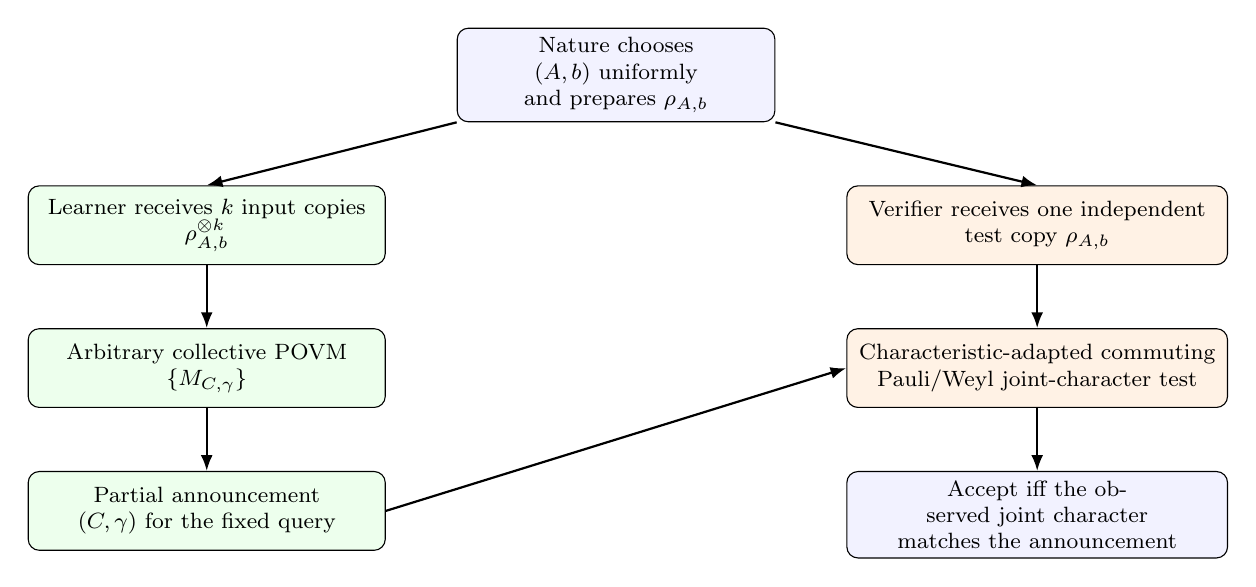
\begin{tikzpicture}[
 font=\footnotesize, node distance=8mm and 9mm,
 source/.style={draw,rounded corners,align=center,minimum height=10mm,text width=38mm,fill=blue!5},
 learner/.style={draw,rounded corners,align=center,minimum height=10mm,text width=43mm,fill=green!7},
 verifier/.style={draw,rounded corners,align=center,minimum height=10mm,text width=46mm,fill=orange!10},
 result/.style={draw,rounded corners,align=center,minimum height=10mm,text width=46mm,fill=blue!5},
 arr/.style={-{Latex[length=2mm]},thick}]
\node[source] (nature) {Nature chooses $(A,b)$ uniformly\\and prepares $\rho_{A,b}$};
\node[learner,below left=of nature] (lin) {Learner receives $k$ input copies\\$\rho_{A,b}^{\otimes k}$};
\node[verifier,below right=of nature] (vin) {Verifier receives one independent\\test copy $\rho_{A,b}$};
\node[learner,below=of lin] (povm) {Arbitrary collective POVM\\$\{M_{C,\gamma}\}$};
\node[learner,below=of povm] (announce) {Partial announcement\\$(C,\gamma)$ for the fixed query};
\node[verifier,below=of vin] (test) {Characteristic-adapted commuting\\Pauli/Weyl joint-character test};
\node[result,below=of test] (accept) {Accept iff the observed joint character\\matches the announcement};
\draw[arr] (nature.south west)--(lin.north);
\draw[arr] (nature.south east)--(vin.north);
\draw[arr] (lin)--(povm); \draw[arr] (povm)--(announce);
\draw[arr] (vin)--(test); \draw[arr] (announce.east)--(test.west);
\draw[arr] (test)--(accept);
\end{tikzpicture}%
}
\caption{Operational structure of finite-copy partial learning for every prime,
shown after the announced reference frame has been sent to the standard
coordinate frame.  In these coordinates, $(C,\gamma)$ is the learner's
announcement for the first $m$ reference-dual stabilizer directions and their
character; the remaining $n-m$ directions are not requested.  Nature supplies
the learner's $k$ systems separately from the verifier's independent test
system, and the verifier performs the characteristic-adapted commuting
joint-character test.  At $m=n$ the acceptance probability equals full-label
fidelity within the complete coordinate ensemble, whereas for $m<n$ it is a
partial verification score.}
\label{fig:prediction-game-protocol}
\end{figure}

\subsection{Score achievable without using the input copies}
\label{subsec:partial-no-information-baseline}
\begin{proposition}[Input-independent score $p^{-m}$]
\label{prop:partial-no-information-baseline}
For every $k\geq0$,
\begin{equation}
 S_{\mathrm{ver}}^{(k),*}(n,m;p)\geq p^{-m}.
 \label{eq:partial-no-information-baseline}
\end{equation}
\end{proposition}

\begin{proof}
Fix $C_0\in\mathcal C_{n,m}$.  On the learner's $k$-copy Hilbert space,
define measurement operators indexed by
$\Theta_{n,m,p}^{\mathrm{part}}=\mathcal C_{n,m}\times\F_p^m$ by
\begin{equation}
 M_{C,\gamma}^{(0)}
 :=
 \begin{cases}
 p^{-m}I,&C=C_0,\\
 0,&C\ne C_0.
 \end{cases}.
 \label{eq:partial-baseline-explicit-POVM}
\end{equation}
Every operator in Eq.~\eqref{eq:partial-baseline-explicit-POVM} is positive.
The sum over all outcomes is normalized because only the fixed matrix label
$C_0$ contributes:
\begin{equation}
 \sum_{C\in\mathcal C_{n,m}}\sum_{\gamma\in\F_p^m}
 M_{C,\gamma}^{(0)}
 =\sum_{\gamma\in\F_p^m}p^{-m}I=I.
 \label{eq:partial-baseline-POVM-normalization}
\end{equation}
Thus Eq.~\eqref{eq:partial-baseline-explicit-POVM} defines a feasible learner POVM.  
Operationally, it ignores the learner's input systems, fixes the matrix label  
$C_0$, and chooses the character label $\gamma$ uniformly.  We now verify that  
its graded score is $p^{-m}$ for every true state, rather than only after  
averaging over the prior.  For a fixed true state $\rho_{A,b}$, the conditional  
graded score is  
\begin{align}
 &\sum_{C\in\mathcal C_{n,m}}\sum_{\gamma\in\F_p^m}
 \Tr\!\left[M_{C,\gamma}^{(0)}\rho_{A,b}^{\otimes k}\right]
 \Tr\!\left[\Pi_{C,\gamma}^{(m)}\rho_{A,b}\right]
 =p^{-m}\sum_{\gamma\in\F_p^m}
 \Tr\!\left[\Pi_{C_0,\gamma}^{(m)}\rho_{A,b}\right]\notag\\
 &\quad=p^{-m}\Tr\!\left[
 \left(\sum_{\gamma\in\F_p^m}\Pi_{C_0,\gamma}^{(m)}\right)
 \rho_{A,b}\right]
 =p^{-m}.
 \label{eq:partial-baseline-average}
\end{align}
The second equality uses
$\Tr[M_{C_0,\gamma}^{(0)}\rho_{A,b}^{\otimes k}]=p^{-m}$, and the last equality
uses the joint-projector resolution of the identity and
$\Tr\rho_{A,b}=1$.  This equality holds for every $(A,b)$, so averaging over
the uniform prior gives the feasible value $p^{-m}$.  Maximizing over all
learner POVMs proves Eq.~\eqref{eq:partial-no-information-baseline}.
For $p=2$, the same input-independent construction uses the binary
joint-character projectors $\Pi_{C,\gamma}^{(m,2)}$ from
Eq.~\eqref{eq:integrated-qubit-accept-projector}; their resolution of the
identity in Eq.~\eqref{eq:integrated-qubit-projector-resolution} gives the
same value $2^{-m}$.
\end{proof}

\subsection{Fixed query subspaces and canonical coordinates}
\label{subsec:query-coordinate-equivalence}

For the odd-prime Weyl realization, the coordinate equivalence can be written explicitly.  The corresponding all-prime
operational conclusion is formulated intrinsically in
Proposition~\ref{prop:frame-conditioned-coordinate-reduction}; the phase-adjusted binary
Pauli realization is not obtained by reusing the Weyl phase convention below.
Within the odd-prime realization, the use of the first $m$ standard generators
is only a coordinate choice.  Let $J\in\F_p^{n\times m}$ have full column rank
and define
\begin{equation}
 \mathcal C_J:=\{C\in\F_p^{n\times m}:J^TC=C^TJ\}.
 \label{eq:general-query-symmetric-matrix-space}
\end{equation}
The associated true label is $(AJ,-J^Tb)$, and the verifier tests the family
$(J;C)$.  Write
\begin{equation}
 \Theta_J:=\mathcal C_J\times\F_p^m,
 \quad
 \Theta_{\rm can}:=\mathcal C_{n,m}\times\F_p^m.
 \label{eq:general-and-canonical-query-label-spaces}
\end{equation}
For $(C,\gamma)\in\Theta_J$, let $\Pi_{C,\gamma}^{(J)}$ denote the joint-character
projector for the Weyl family $\{W(Jx,Cx):x\in\F_p^m\}$.  For $y\in\Theta_J$,
let $\sigma_y^{(J)}$ be the $k$-copy state obtained by averaging
$\rho_{A,b}^{\otimes k}$ over the complete coordinate labels $(A,b)$ satisfying
$(AJ,-J^Tb)=y$.  The superscript $(J_m)$ denotes the corresponding canonical
objects.

\subsubsection{Label, state, and measurement correspondences}
\label{subsubsec:fixed-query-correspondences}

\begin{proposition}[Explicit equivalence of fixed full-rank queries]
\label{prop:fixed-query-equivalence}
Let $J\in\F_p^{n\times m}$ have full column rank.  Choose
$R\in\operatorname{GL}(n,\F_p)$ such that $J=RJ_m$, and define
\begin{equation}
 T_R:\Theta_J\longrightarrow\Theta_{\rm can},
 \quad
 T_R(C,\gamma):=(R^TC,\gamma).
 \label{eq:fixed-query-label-map}
\end{equation}
Then $T_R$ is a bijection with inverse
\begin{equation}
 T_R^{-1}(C',\gamma)=(R^{-T}C',\gamma).
 \label{eq:fixed-query-label-map-inverse}
\end{equation}
The change of query frame induces a corresponding transformation of every
complete coordinate label in the transverse model.  For $(A,b)$, denote the transformed label by $(A',b')$, where
\begin{equation}
 A':=R^TAR,
 \quad b':=R^Tb.
 \label{eq:fixed-query-transformed-complete-label}
\end{equation}
The true queried labels obey
\begin{equation}
 T_R(AJ,-J^Tb)=(A'J_m,-J_m^Tb').
 \label{eq:fixed-query-true-label-correspondence}
\end{equation}
The same change of frame is implemented quantumly by the computational-basis
unitary $U_R\ket{x}:=\ket{R^{-1}x}$.  It intertwines both the verifier
projectors and the conditioned learner states.  For
$y=(C,\gamma)\in\Theta_J$, the two correspondence relations are
\begin{align}
 U_R\Pi_{C,\gamma}^{(J)}U_R^\dagger
 =\Pi_{T_R(y)}^{(J_m)},~
 U_R^{\otimes k}\sigma_y^{(J)}U_R^{\dagger\otimes k}
 =\sigma_{T_R(y)}^{(J_m)}.
 \label{eq:fixed-query-projector-correspondence}
\end{align}
Consequently, conjugation by $U_R^{\otimes k}$ together with the label map
$T_R$ gives a bijection between the feasible learner POVMs for the $J$-query
problem and those for the canonical $J_m$-query problem.  It preserves every
exact-identification term and every graded-score term.  Therefore the optimal
exact-identification probability and the optimal graded-verification score for
query $J$ equal, respectively,
$P_{\mathrm{id}}^{(k),*}(n,m;p)$ and $S_{\mathrm{ver}}^{(k),*}(n,m;p)$.
\end{proposition}

\begin{proof}
First verify the domains in Eqs.~\eqref{eq:fixed-query-label-map} and
\eqref{eq:fixed-query-label-map-inverse}.  If $C\in\mathcal C_J$, then
\begin{equation}
 J_m^T(R^TC)=J^TC=C^TJ=(R^TC)^TJ_m,
 \label{eq:fixed-query-forward-admissibility}
\end{equation}
so $R^TC\in\mathcal C_{n,m}$.  The inverse transformation also preserves
admissibility.  Specifically, if $C'\in\mathcal C_{n,m}$, then
\begin{equation}
 J^T(R^{-T}C')=J_m^TC'=C'^TJ_m=(R^{-T}C')^TJ,
 \label{eq:fixed-query-inverse-admissibility}
\end{equation}
so $R^{-T}C'\in\mathcal C_J$.  The two displayed maps are inverse because
$R^{-T}R^T=I$.  This proves the asserted bijection, including its domain,
codomain, forward map, and inverse.

Applying $U_R\ket{x}=\ket{R^{-1}x}$ and changing the summation variable
from $x$ to $Rx$ gives
\begin{equation}
 U_R\ket{\psi_{A,b}}=\ket{\psi_{R^TAR,R^Tb}}
 =\ket{\psi_{A',b'}}.
 \label{eq:fixed-query-state-correspondence}
\end{equation}
Since $J=RJ_m$, Eq.~\eqref{eq:fixed-query-transformed-complete-label} gives
\begin{equation}
 R^TAJ=R^TARJ_m=A'J_m,
 \quad
 J^Tb=J_m^TR^Tb=J_m^Tb',
 \label{eq:fixed-query-true-coordinate-calculation}
\end{equation}
which proves Eq.~\eqref{eq:fixed-query-true-label-correspondence}.

The action of $U_R$ on computational-basis states determines its conjugation
action on the shift and phase operators.  For all $u,v\in\F_p^n$, one has
\begin{align}
 U_RX(u)U_R^\dagger=X(R^{-1}u),~
 U_RZ(v)U_R^\dagger=Z(R^Tv).
 \label{eq:fixed-query-Z-conjugation}
\end{align}
Moreover $(R^{-1}u)^T(R^Tv)=u^Tv$, so the phase
$\omega^{-u^Tv/2}$ in the Weyl convention is preserved.  Combining this phase
invariance with the two conjugation identities gives the Weyl-operator
correspondence
\begin{equation}
 U_RW(u,v)U_R^\dagger=W(R^{-1}u,R^Tv).
 \label{eq:fixed-query-general-Weyl-conjugation}
\end{equation}
For $u=Jx=RJ_mx$, $v=Cx$, and $C'=R^TC$, this becomes
\begin{equation}
 U_RW(Jx,Cx)U_R^\dagger=W(J_mx,C'x).
 \label{eq:query-coordinate-Weyl-family}
\end{equation}
Substituting Eq.~\eqref{eq:query-coordinate-Weyl-family} into the character-sum
definition of the joint projector proves
Eq.~\eqref{eq:fixed-query-projector-correspondence}.  The transformation
$(A,b)\mapsto(A',b')$ is a bijection of the uniform complete-label space, and
Eq.~\eqref{eq:fixed-query-true-label-correspondence} maps the fiber over
$y\in\Theta_J$ bijectively onto the fiber over $T_R(y)$.  Conjugating each term
in the fiber average by $U_R^{\otimes k}$ therefore proves
Eq.~\eqref{eq:fixed-query-projector-correspondence}.

Finally, for a $J$-query POVM $\{M_y:y\in\Theta_J\}$ define the canonical POVM
by
\begin{equation}
 \widetilde M_{T_R(y)}
 :=U_R^{\otimes k}M_yU_R^{\dagger\otimes k}.
 \label{eq:fixed-query-POVM-correspondence}
\end{equation}
Positivity and normalization are preserved, and the inverse construction uses
$T_R^{-1}$ and $U_R^{\dagger\otimes k}$.  Hence
Eq.~\eqref{eq:fixed-query-POVM-correspondence} is a bijection of feasible POVMs.
Equation~\eqref{eq:fixed-query-state-correspondence} preserves the
probability of each relabeled learner outcome.  Equation
\eqref{eq:fixed-query-projector-correspondence} preserves the verifier's
conditional acceptance probability.  Thus exact success and graded score are
preserved term by term, and taking the two optima proves the final assertion.
\end{proof}

The preceding equivalence also completes the connection with the announced
reference frame.  The opening reduction of this section treats that frame by a
publicly specified symplectic coordinate change, while
Proposition~\ref{prop:fixed-query-equivalence} shows, within the odd-prime
realization, that replacing the canonical inclusion $J_m$ by any fixed
full-rank query preserves every exact and graded term.  Together with
Proposition~\ref{prop:frame-conditioned-coordinate-reduction}, this completes
the passage from the intrinsic frame-relative task to the canonical formulas
used below.
\subsection{The full-label fidelity endpoint \texorpdfstring{$m=n$}{m=n}}
\label{subsec:complete-endpoint}
At $m=n$, the queried coordinate label becomes complete within the ensemble
conditioned on the announced frame.  This is still not the unrestricted
stabilizer ensemble of Eqs.~\eqref{eq:unrestricted-stabilizer-wc-success} and~\eqref{eq:unrestricted-stabilizer-av-success}, which is
used separately as the direct benchmark.  Exact identification tests equality
of complete coordinate labels, whereas the graded payoff becomes the squared
overlap with the announced coordinate state; accordingly, the two finite
optima need not coincide.  The characteristic-specific score formulas established above ensure only
that score one is attained exactly by the correct label.

\begin{definition}[Full-label fidelity learning]
At the endpoint $m=n$, the learner outputs a complete coordinate label
$(A',b')$.  Against the true label $(A,b)$, the score is
\begin{equation}
 \left|\braket{\psi_{A',b'}}{\psi_{A,b}}\right|^2.
 \label{eq:full-label-fidelity-score}
\end{equation}
We call this the full-label fidelity-learning problem, and denote its optimal
average score by $P_{\mathrm{succ}}^{(k),*}(n,p)$.  Despite the letter $P$,
this endpoint notation denotes a graded fidelity score, not an
exact-identification probability.
\end{definition}
\begin{corollary}[Recovery of full-label fidelity learning]
\label{cor:complete-fidelity-endpoint}
If $m=n$, then $J_n=I_n$,
$\mathcal C_{n,n}=\Sym_n(\F_p)$, and an announcement can be written uniquely
as $(C,\gamma)=(A',-b')$.  Under this identification, the verifier score
coincides exactly with the fidelity between the two complete-label states:
\begin{equation}
 s_n((A,b),(A',-b'))
 =\left|\braket{\psi_{A',b'}}{\psi_{A,b}}\right|^2.
 \label{eq:partial-score-complete-fidelity}
\end{equation}
For odd $p$, this identification is the symmetric-matrix coordinate statement
shown above.  For $p=2$, the same conclusion uses the enhanced binary
complete-label coordinates and the binary rank-one projector construction;
it is not obtained by applying the odd-prime Weyl phase formula verbatim.
In both cases the unreported subgroup is trivial when $m=n$, so the quotient
is the full label group.  The announcement is therefore a complete label,
and its accept projector is the corresponding pure-state projector.

The two optimization problems therefore have the same objective on the same
complete-label output alphabet.  Their optimal values are equal:
\begin{equation}
 S_{\mathrm{ver}}^{(k),*}(n,n;p)
 =P_{\mathrm{succ}}^{(k),*}(n,p),
 \label{eq:partial-complete-optimal-equality}
\end{equation}
where the right-hand side is the full-label fidelity-learning optimum.
\end{corollary}

\begin{proof}
For $m=n$, Eq.~\eqref{eq:partial-accept-projector} is the rank-one projector
onto $\ket{\psi_{A',b'}}$ when $(C,\gamma)=(A',-b')$.  Equation
\eqref{eq:partial-score-complete-fidelity} follows from Born's rule, and the
feasible measurements and priors are identical under this relabeling.
\end{proof}



\section{Finite-size exact identification}
\label{sec:common-finite-size-framework}
We now solve the finite exact-identification problem for the refined task.
The states conditioned on a partial label are mixed, so covariance alone does
not determine an optimal measurement.  After formulating the quotient
ensemble, we decompose the $k$-copy pure states into odd-prime or enhanced binary
moment sectors.  Averaging over the unreported coordinates leaves orthogonal
rank-one coherence blocks.  A common seed semidefinite program then exploits
these blocks to prove PGM optimality and obtain the exact finite-copy formula
used in the converse.

\subsection{Quotient formulation and proof architecture}
\label{subsec:finite-size-quotient-architecture}

We now introduce the canonical quotient notation used in the proof.  Let
$G_{n,p}$ be the additive complete-label group and $H_{n,m,p}$ the subgroup of
unreported coordinates.  For odd $p$,
\begin{equation}
 H_{n,m,p}:=\left\{\left(\begin{pmatrix}0&0\\0&F\end{pmatrix},
 \binom{0}{c}\right):F\in\Sym_{n-m}(\F_p),\ c\in\F_p^{n-m}\right\}.
 \label{eq:H}
\end{equation}
For $p=2$ its enhanced-coordinate version is
Eq.~\eqref{eq:integrated-qubit-unreported-subgroup}.  Put
$Y_{n,m,p}:=G_{n,p}/H_{n,m,p}$.  For $g\in G_{n,p}$, let $\rho_g$
denote the pure coordinate stabilizer state associated with the complete
additive label $g$.  Thus $\rho_g=\rho_{A,b}$ in odd characteristic and is
the state associated with $\ket{\psi_g^{(2)}}$ in characteristic two.  We have
\begin{equation}
 |Y_{n,m,p}|=p^{(n+1)m-m(m-1)/2}.
 \label{eq:Y-size}
\end{equation}
For $y\in Y_{n,m,p}$, define the conditioned state
\begin{equation}
 \sigma_y:=\frac1{|H_{n,m,p}|}\sum_{h\in H_{n,m,p}}
 \rho_{s_Y(y)+h}^{\otimes k},
 \label{eq:sigma-y}
\end{equation}
where $s_Y(y)$ is any quotient representative.  Also set
\begin{equation}
 \kappa_p^{\mathrm{GL}}:=\prod_{j=1}^{\infty}(1-p^{-j})>0.
 \label{eq:kappa-GL-product}
\end{equation}

The refined operational reduction is now complete.  The proof has three steps.  
First, the characteristic-specific moment maps identify the aggregate data on  
which the complete-label phases depend.  Second, averaging over the unreported  
subgroup determines which moment sectors retain mutual coherence and groups  
them into annihilator-coset blocks.  Third, a characteristic-independent seed  
semidefinite program optimizes those blocks.  The first two steps require  
separate odd-prime and binary realizations, whereas the final optimization is  
common.  The following table summarizes this division of roles.  All results  
in this section are finite-copy statements.  
\begin{center}
\small
\setlength{\tabcolsep}{7pt}
\renewcommand{\arraystretch}{1.22}
\begin{tabularx}{0.96\textwidth}{@{}>{\raggedright\arraybackslash}p{0.20\textwidth}YY@{}}
\toprule
\textbf{Layer}
& \textbf{Odd-prime realization}
& \textbf{Characteristic-two realization}\\
\midrule
\textbf{Additive parameters}
& $\Sym_n(\F_p)\times\F_p^n$
& $\mathbb Z_4^n\times\F_2^{\binom n2}$\\
\addlinespace[1pt]
\textbf{Moment data}
& Symmetric Gram moment and linear moment
& Mod-$4$ diagonal and mod-$2$ off-diagonal moments\\
\addlinespace[1pt]
\textbf{Fixed lower-coordinate blocks}
& $H^\perp$-cosets indexed by $(Q_{22},S_2)$
& Annihilator cosets of the enhanced moment group\\
\addlinespace[1pt]
\textbf{Common finite-size conclusion}
& \multicolumn{2}{>{\raggedright\arraybackslash}p{0.70\textwidth}@{}}{Fixed-diagonal block of the seeds, rank-one optimizer, exact coset formula, and PGM optimality}\\
\bottomrule
\end{tabularx}
\end{center}

\subsection{Odd-prime moment realization}
\label{sec:sectors}
For odd $p$, computational-basis tuples decompose into moment sectors, and averaging over the unreported subgroup preserves coherence exactly within the blocks identified below.  The optimization itself is postponed to
Section~\ref{sec:seed-sdp}; no success-probability bound is taken here.

\subsubsection{The quotient ensemble and the moment map}
The first task is to replace the computational-basis expansion, whose terms are indexed by $k$ vectors, by a decomposition indexed by the aggregate data on which the label-dependent phase actually depends.  This removes the irrelevant ordering information while retaining the complete character carried by each group orbit.  Recall the additive parameter group $G=\Sym_n(\F_p)\times\F_p^n$, the unreported
subgroup $H$ in Eq.~\eqref{eq:H}, the partial-label quotient $Y=G/H$, and the
conditioned states $\{\sigma_y:y\in Y\}$ in Eq.~\eqref{eq:sigma-y}.  We first
introduce coordinates that diagonalize the $G$-action.

\begin{definition}[Moment values, fibers, and normalized sector vectors]
An ordered computational-basis tuple in the $k$-copy expansion is an element
\begin{equation}
 \boldsymbol x=(x_1,\ldots,x_k)\in(\F_p^n)^k.
 \label{eq:ordered-basis-tuple-domain}
\end{equation}
Define its moment value by the map
\begin{equation}
 \Phi_k:(\F_p^n)^k\longrightarrow
 \Sym_n(\F_p)\times\F_p^n,
 \quad
 \Phi_k(\boldsymbol x)
 :=\left(\sum_{j=1}^k x_jx_j^T,\ \sum_{j=1}^k x_j\right).
 \label{eq:moment-map}
\end{equation}
For $z=(Q,S)\in G$, define the preimage of a moment value and its cardinality by
\begin{equation}
 \Phi_k^{-1}(z)
 :=\{\boldsymbol x\in(\F_p^n)^k:\Phi_k(\boldsymbol x)=z\},
 \quad
 N_z:=|\Phi_k^{-1}(z)|.
 \label{eq:moment-fiber-and-cardinality}
\end{equation}
We say that $z$ \emph{occurs at copy number $k$} when any, and hence all, of
the following equivalent conditions hold:
\begin{equation}
 z\in\operatorname{im}\Phi_k,
 \quad
 \Phi_k^{-1}(z)\ne\varnothing,
 \quad
 N_z>0.
 \label{eq:occurring-moment-equivalences}
\end{equation}
For every occurring moment value, put
\begin{equation}
 |v_z\rangle
 :=\sum_{\boldsymbol x\in\Phi_k^{-1}(z)}|\boldsymbol x\rangle,
 \quad
 |e_z\rangle:=N_z^{-1/2}|v_z\rangle.
 \label{eq:fiber-sector}
\end{equation}
The one-dimensional space $\operatorname{span}\{|e_z\rangle\}$ is the
\emph{moment sector at $z$}.  The common orbit support is
\begin{equation}
 \mathcal K_{k,n}
 :=\operatorname{span}\{|e_z\rangle:z\in\operatorname{im}\Phi_k\}.
 \label{eq:orbit-support}
\end{equation}
Thus the moment sectors in $\mathcal K_{k,n}$ are indexed exactly by the
moment values that occur at copy number $k$.
\end{definition}
Here $N_z$ is the multiplicity of one moment value in the ordered-tuple
expansion, while $|e_z\rangle$ is the normalized direction carrying its
character.  The vectors $|e_z\rangle$ are orthonormal because distinct fibers
of $\Phi_k$ are disjoint.

Use the character pairing
\begin{equation}
 \chi_{(Q,S)}(A,b):=\omega^{\frac12\Tr(AQ)+b^TS}.       \label{eq:pairing}.
\end{equation}
The factor $1/2$ compensates for the doubling of off-diagonal entries in the
trace pairing on symmetric matrices.

\begin{lemma}[Moment expansion of the orbit states]
\label{lem:orbit-moment-expansion}
For $g=(A,b)\in G$,
\begin{equation}
 |\Psi_g\rangle:=|\psi_g\rangle^{\otimes k}
 =p^{-nk/2}\sum_{z\in\operatorname{im}\Phi_k}
 \sqrt{N_z}\,\chi_z(g)|e_z\rangle.              \label{eq:orbit-sector-expansion}.
\end{equation}
\end{lemma}
\begin{proof}
Expand $|\psi_g\rangle^{\otimes k}$ in the computational basis.  The phase
of an ordered basis tuple $(x_1,\ldots,x_k)$ depends on that tuple only through
$\Phi_k(x_1,\ldots,x_k)$.  Partitioning the basis tuples into the fibers in
Eq.~\eqref{eq:moment-fiber-and-cardinality} gives the stated expansion, with
coefficient $\sqrt{N_z}$ after normalization.
\end{proof}

\subsubsection{Moment coordinates associated with unreported parameters}
The moment expansion alone does not yet reflect the partial nature of the learning problem.  We must next determine which coherences survive when labels differing only in unreported coordinates are averaged together.  The answer is expressed by the restriction of a moment character to the unreported subgroup.  The terminology used below is relative to the requested partial label.  Write
the odd-prime symmetric-matrix parameters as
\begin{equation}
 A=\begin{pmatrix}A_{11}&A_{12}\\A_{12}^T&A_{22}\end{pmatrix},
 \quad b=\binom{b_1}{b_2}.
 \label{eq:finite-size-parameter-split}
\end{equation}
For the canonical query, the partial label records $(A_{11},A_{12}^T,b_1)$
and does not record $(A_{22},b_2)$.  The subgroup $H$ in Eq.~\eqref{eq:H} is
therefore the kernel of the partial-label homomorphism: its translations vary
only $(A_{22},b_2)$ and leave the requested label unchanged.

Under the character pairing in Eq.~\eqref{eq:pairing}, the parameter block
$(A_{22},b_2)$ pairs with the moment block $(Q_{22},S_2)$.  Consequently,
averaging an orbit state over $H$ preserves a matrix element between moment
values $z$ and $z'$ exactly when the characters $\chi_z$ and $\chi_{z'}$ have
the same restriction to $H$.  The next definition and lemma express this
condition as equality of the lower moment coordinates.  Let $\1_k\in\F_p^k$ denote the all-ones column vector.  All subsequent
statements use the coordinate map $r$, its fibers, and the explicit event
$(X_2X_2^T,X_2\1_k)=\zeta$; no information-theoretic notion of observability
is required.

\begin{definition}[Coordinate invariant of the $H^\perp$-cosets]
Let
\begin{equation}
 H^\perp:=\{z\in G:\chi_z(h')=1\text{ for every }h'\in H\}.
 \label{eq:odd-annihilator-definition}
\end{equation}
For
\begin{equation}
 Q=\begin{pmatrix}Q_{11}&Q_{12}\\Q_{12}^T&Q_{22}\end{pmatrix},
 \quad S=\binom{S_1}{S_2},
 \label{eq:moment-coordinate-split}
\end{equation}
define
\begin{equation}
 r:G\longrightarrow\Sym_{n-m}(\F_p)\times\F_p^{n-m},
 \quad r(Q,S):=(Q_{22},S_2).
 \label{eq:unreported-moment-early}
\end{equation}
We write $\zeta=r(z)$.  Thus $\zeta$ is the value of the explicit coordinate
map $r$, not an additional information-theoretic notion.
\end{definition}

\begin{lemma}[Coordinate description of the $H^\perp$-cosets]
\label{lem:unreported-moment-cosets}
The map $r$ in Eq.~\eqref{eq:unreported-moment-early} satisfies
\begin{equation}
 H^\perp=\ker r
 =\{(Q,S):Q_{22}=0,\ S_2=0\},
 \quad |H^\perp|=|G/H|=\lvert Y\rvert.
 \label{eq:H-perp}
\end{equation}
For $z,z'\in G$,
\begin{equation}
 z-z'\in H^\perp
 \quad\Longleftrightarrow\quad
 r(z)=r(z').
 \label{eq:coset-coordinate-equivalence}
\end{equation}
Hence, for every $\zeta=(\zeta_Q,\zeta_S)$ in the image of $r$, the associated
coset is the explicitly defined fiber
\begin{equation}
 \mathcal C_{\zeta}:=r^{-1}(\zeta)
 =\{(Q,S)\in G:Q_{22}=\zeta_Q,\ S_2=\zeta_S\}.
 \label{eq:coset-as-coordinate-fiber}
\end{equation}
These fibers are exactly the $H^\perp$-cosets in $G$.
\end{lemma}
\begin{proof}
For an element $h'\in H$ with lower parameter blocks $(F,c)$,
\begin{equation}
 \chi_{(Q,S)}(h')
 =\omega^{\frac12\Tr(FQ_{22})+c^TS_2}.
 \label{eq:annihilator-lower-block-pairing}
\end{equation}
This character equals one for every symmetric $F$ and every $c$ if and only if
$Q_{22}=0$ and $S_2=0$.  This proves $H^\perp=\ker r$ and
Eq.~\eqref{eq:H-perp}.  Since $r$ is linear,
$z-z'\in\ker r$ if and only if $r(z)=r(z')$, proving
Eq.~\eqref{eq:coset-coordinate-equivalence}.  Equation
\eqref{eq:coset-as-coordinate-fiber} is then the coordinate description of
the corresponding coset.
\end{proof}

\begin{definition}[Coset vectors, total fiber size, and occurring moment values]
For $\zeta$ in the image of $r$, define
\begin{align}
 |w_{\zeta}\rangle
 &:=\sum_{z\in\mathcal C_{\zeta}\cap\operatorname{im}\Phi_k}
       \sqrt{N_z}|e_z\rangle,&
 |u_{\zeta}\rangle
 &:=\sum_{z\in\mathcal C_{\zeta}\cap\operatorname{im}\Phi_k}|e_z\rangle,
 \label{eq:w-u}\\
 T_{\zeta}
 &:=\sum_{z\in\mathcal C_{\zeta}}N_z,&
 d_{\zeta}
 &:=|\mathcal C_{\zeta}\cap\operatorname{im}\Phi_k|.
 \label{eq:early-Th-dh}
\end{align}
The integer $T_{\zeta}$ counts the ordered computational-basis tuples
$\boldsymbol x\in(\F_p^n)^k$ whose moment value lies in
$\mathcal C_{\zeta}$:
\begin{equation}
 T_{\zeta}
 =|\{\boldsymbol x\in(\F_p^n)^k:
       \Phi_k(\boldsymbol x)\in\mathcal C_{\zeta}\}|.
 \label{eq:T-zeta-counted-set}
\end{equation}
The integer $d_{\zeta}$ counts the full moment values in that coset that occur
at copy number $k$.  Thus $T_{\zeta}$ is the total tuple mass in one surviving
coherence block, whereas $d_{\zeta}$ is the number of distinct occurring
moment values above the same lower coordinate.

Because $r(z)=\zeta$ fixes $(Q_{22},S_2)$, the map
\begin{equation}
 (Q,S)\longmapsto(Q_{11},Q_{12},S_1).
 \label{eq:coset-to-remaining-coordinate-map}
\end{equation}
is injective on $\mathcal C_{\zeta}$ and identifies
$\mathcal C_{\zeta}\cap\operatorname{im}\Phi_k$ with the set of remaining
coordinate triples arising from some ordered basis tuple.  Moreover,
\begin{equation}
 z\longmapsto\operatorname{span}\{|e_z\rangle\}.
 \label{eq:occurring-moment-to-sector-map}
\end{equation}
is a bijection from
$\mathcal C_{\zeta}\cap\operatorname{im}\Phi_k$ onto the nonzero moment
sectors in this coset.  Thus $d_{\zeta}$ has the three equivalent, explicitly
related interpretations: occurring full moment values, occurring remaining
coordinate triples, and nonzero moment sectors.
\end{definition}

\subsubsection{Conditioned and average states in moment coordinates}
The preceding definitions convert subgroup averaging into equality of the lower moment coordinate $r(z)$.  Translating this character-theoretic condition into the density operators yields the ensemble used for minimum-error discrimination.  The next proposition gives the odd-prime block structure used in the common seed optimization.

\begin{proposition}[Block form of the exact-identification ensemble]
\label{prop:conditioned-average-block-form}
For the zero partial label,
\begin{equation}
 \sigma_0=p^{-nk}\sum_{\zeta}|w_{\zeta}\rangle\!\langle w_{\zeta}|.          \label{eq:sigma-zero-blocks}.
\end{equation}
The blocks indexed by distinct fibers of $r$ are mutually orthogonal.  The
uniform ensemble average is
\begin{equation}
 \overline\sigma:=\frac1{\lvert Y\rvert}\sum_{y\in Y}\sigma_y
 =p^{-nk}\sum_{z:N_z>0}N_z|e_z\rangle\!\langle e_z|,      \label{eq:average-state},
\end{equation}
and hence, on $\mathcal K_{k,n}$,
\begin{equation}
 \overline\sigma^{-1/2}
 =p^{nk/2}\sum_{z:N_z>0}N_z^{-1/2}|e_z\rangle\!\langle e_z|.
                                                        \label{eq:average-inverse}
\end{equation}
\end{proposition}
\begin{proof}
Insert Eq.~\eqref{eq:orbit-sector-expansion} into the definition of $\sigma_0$.
Averaging over $H$ annihilates the matrix element $(z,z')$ unless
$z-z'\in H^\perp$.  By
Eq.~\eqref{eq:coset-coordinate-equivalence}, this is exactly the condition
$r(z)=r(z')$, which establishes Eq.~\eqref{eq:sigma-zero-blocks}.  Averaging over
the whole quotient, equivalently over $G$, leaves only $z=z'$ by character
orthogonality and gives Eq.~\eqref{eq:average-state}.  Functional calculus on
its support gives Eq.~\eqref{eq:average-inverse}.
\end{proof}

The odd-prime conditioned ensemble has therefore been reduced to mutually  
orthogonal annihilator-coset blocks with explicitly defined multiplicities.  
This block form is the structural input needed by the common optimization.  
The quantities $T_{\zeta}$ and $d_{\zeta}$ will later become, respectively, a  
lower-event probability mass and an occurring-moment count in the converse.  


\subsection{Characteristic-two moment realization}
\label{sec:integrated-qubit-moments}
In characteristic two, the enhanced quadratic phase produces mixed mod-$4$/mod-$2$ moment coordinates.  Nevertheless, the resulting conditioned states again decompose into orthogonal annihilator-coset blocks, with one multiplicity for each occurring moment value.

\subsubsection{Moment group and character pairing in characteristic two}
The binary argument follows the same logic as the odd-prime construction, but its aggregate data cannot be represented by an ordinary symmetric Gram matrix alone.  The diagonal phase is naturally modulo four, while off-diagonal products remain modulo two.  We therefore first build the character group in which these two kinds of data coexist.  Let
\begin{equation}
 \mathcal M_{n,2}:=\mathbb Z_4^n\times
 \F_2^{\binom n2}.
 \label{eq:binary-enhanced-moment-group}
\end{equation}
We write a parameter as $g=(\alpha,E)\in G_{n,2}$, with
$\alpha=(\alpha_a)_{a=1}^n\in\mathbb Z_4^n$ and
$E=(E_{ab})_{a<b}\in\F_2^{\binom n2}$, and a moment value as
$z=(r,T)\in\mathcal M_{n,2}$, with the same respective coordinate groups.
Define the character pairing by
\begin{equation}
 \chi_z^{(2)}(g)
 :=i^{\sum_{a=1}^n\alpha_a r_a}
   (-1)^{\sum_{1\le a<b\le n}E_{ab}T_{ab}}.
 \label{eq:binary-enhanced-character-pairing}
\end{equation}
The first exponent is evaluated modulo $4$ and the second modulo $2$.
The pairing is nondegenerate: summing $\chi_z^{(2)}(g)$ over all
$g\in G_{n,2}$ gives $|G_{n,2}|$ when $z=0$ and zero otherwise.
Thus $\mathcal M_{n,2}$ is identified explicitly with the character group
$\widehat G_{n,2}$.

For an ordered computational-basis tuple
$\boldsymbol x=(x_1,\ldots,x_k)\in(\F_2^n)^k$, define
\begin{equation}
 \Phi_k^{(2)}(\boldsymbol x):=(r(\boldsymbol x),T(\boldsymbol x))
 \in\mathcal M_{n,2},
 \label{eq:integrated-qubit-moment-map}
\end{equation}
where
\begin{align}
 r_a(\boldsymbol x)&:=\sum_{j=1}^k(x_j)_a\pmod4,
 \label{eq:integrated-qubit-linear-moment}\\
 T_{ab}(\boldsymbol x)&:=\sum_{j=1}^k(x_j)_a(x_j)_b\pmod2,
 \quad a<b.
 \label{eq:integrated-qubit-edge-moment}
\end{align}

\begin{lemma}[Tuple phase factors through the enhanced moment]
\label{lem:binary-tuple-phase-factorization}
For every $g=(\alpha,E)\in G_{n,2}$ and every ordered tuple
$\boldsymbol x\in(\F_2^n)^k$,
\begin{equation}
 \prod_{j=1}^k
 i^{\sum_a\alpha_a(x_j)_a+2\sum_{a<b}E_{ab}(x_j)_a(x_j)_b}
 =\chi_{\Phi_k^{(2)}(\boldsymbol x)}^{(2)}(g).
 \label{eq:binary-tuple-phase-factorization}
\end{equation}
\end{lemma}
\begin{proof}
Multiplying the $k$ phase factors adds their exponents modulo $4$ and gives
\begin{align}
 i^{\sum_a\alpha_a\sum_j(x_j)_a}
  i^{2\sum_{a<b}E_{ab}\sum_j(x_j)_a(x_j)_b}
 =i^{\sum_a\alpha_a r_a(\boldsymbol x)}
  (-1)^{\sum_{a<b}E_{ab}T_{ab}(\boldsymbol x)},
 \label{eq:binary-tuple-phase-calculation}
\end{align}
which is the right-hand side of
Eq.~\eqref{eq:binary-tuple-phase-factorization} by
Eq.~\eqref{eq:binary-enhanced-character-pairing}.
\end{proof}

\subsubsection{Fibers of the characteristic-two moment map and orbit expansion}
Having identified the phase of each tuple with a character of the enhanced moment group, we may now collect all tuples carrying the same character.  This is the binary counterpart of the odd-prime sector decomposition and will provide the orthogonal directions used in the conditioned states.  For $z\in\mathcal M_{n,2}$ define
\begin{equation}
 \mathcal F_z^{(2)}
 :=\{\boldsymbol x\in(\F_2^n)^k:
          \Phi_k^{(2)}(\boldsymbol x)=z\},
 \quad
 N_z^{(2)}:=|\mathcal F_z^{(2)}|.
 \label{eq:binary-enhanced-moment-fiber}
\end{equation}
Call $z$ occurring when $N_z^{(2)}>0$.  For every occurring $z$, put
\begin{equation}
 \ket{e_z^{(2)}}
 :=(N_z^{(2)})^{-1/2}
   \sum_{\boldsymbol x\in\mathcal F_z^{(2)}}\ket{\boldsymbol x},
 \quad
 \mathcal K_{k,n}^{(2)}
 :=\operatorname{span}\{\ket{e_z^{(2)}}:N_z^{(2)}>0\}.
 \label{eq:integrated-qubit-sector-vector}
\end{equation}
Here $N_z^{(2)}$ is the multiplicity of the enhanced moment $z$, and
$\ket{e_z^{(2)}}$ is the normalized character-sector direction carrying that
moment.  Distinct fibers are disjoint, so the occurring sector vectors are
orthonormal.

\begin{lemma}[Moment expansion of the binary orbit states]
\label{lem:binary-orbit-moment-expansion}
For $g=(\alpha,E)\in G_{n,2}$,
\begin{equation}
 \ket{\Psi_g^{(2)}}
 :=\ket{\psi_g^{(2)}}^{\otimes k}
 =2^{-nk/2}\sum_{z:N_z^{(2)}>0}
   \sqrt{N_z^{(2)}}\,\chi_z^{(2)}(g)\ket{e_z^{(2)}}.
 \label{eq:integrated-qubit-orbit-expansion}
\end{equation}
\end{lemma}
\begin{proof}
Expand the tensor power in the ordered computational basis.  By
Lemma~\ref{lem:binary-tuple-phase-factorization}, all tuples in the fiber
$\mathcal F_z^{(2)}$ have the common phase $\chi_z^{(2)}(g)$.
Partitioning the tuples by their moment value and replacing the uniform sum
on each nonempty fiber by
$\sqrt{N_z^{(2)}}\ket{e_z^{(2)}}$ gives
Eq.~\eqref{eq:integrated-qubit-orbit-expansion}.
\end{proof}

\subsubsection{The kernel of the partial-label map and explicit annihilator cosets}
We next impose the distinction between reported and unreported coordinates.  Averaging over the latter preserves a matrix element precisely when the two enhanced moments define the same character on the unreported subgroup.  The restriction map below records exactly the coordinates needed to test this condition.  Split the enhanced moment coordinates according to the queried indices
$1,\ldots,m$ and the lower indices $m+1,\ldots,n$.  Define
\begin{equation}
 \mathcal L_{n,m,2}
 :=\mathbb Z_4^{n-m}\times
   \F_2^{\binom{n-m}{2}},
 \label{eq:binary-lower-moment-space}
\end{equation}
and the restriction map
\begin{equation}
 r_2:\mathcal M_{n,2}\longrightarrow\mathcal L_{n,m,2},
 \quad
 r_2(r,T)
 :=\bigl((r_a)_{a>m},(T_{ab})_{m<a<b\le n}\bigr).
 \label{eq:binary-lower-moment-restriction}
\end{equation}
For $\zeta\in\mathcal L_{n,m,2}$ set
\begin{equation}
 \mathcal C_\zeta^{(2)}:=r_2^{-1}(\zeta).
 \label{eq:binary-annihilator-coset-fiber}
\end{equation}

\begin{lemma}[Coordinate description of the binary annihilator cosets]
\label{lem:binary-annihilator-cosets}
Under the pairing in Eq.~\eqref{eq:binary-enhanced-character-pairing},
\begin{equation}
 H_{n,m,2}^\perp=\ker r_2.
 \label{eq:binary-annihilator-kernel}
\end{equation}
Consequently, for $z,z'\in\mathcal M_{n,2}$,
\begin{equation}
 z-z'\in H_{n,m,2}^\perp
 \quad\Longleftrightarrow\quad
 r_2(z)=r_2(z'),
 \label{eq:binary-annihilator-coset-equivalence}
\end{equation}
and the fibers $\mathcal C_\zeta^{(2)}$ are exactly the
$H_{n,m,2}^\perp$-cosets in $\mathcal M_{n,2}$.
\end{lemma}
\begin{proof}
An element $h\in H_{n,m,2}$ has arbitrary lower coordinates
$\alpha_a$ for $a>m$ and arbitrary lower--lower edge coordinates $E_{ab}$
for $m<a<b\le n$, with all other coordinates zero.  Hence
\begin{equation}
 \chi_{(r,T)}^{(2)}(h)
 =i^{\sum_{a>m}\alpha_a r_a}
  (-1)^{\sum_{m<a<b\le n}E_{ab}T_{ab}}.
 \label{eq:binary-unreported-subgroup-pairing}
\end{equation}
This equals one for every $h\in H_{n,m,2}$ if and only if every lower
$r_a$ is zero modulo $4$ and every lower--lower $T_{ab}$ is zero modulo $2$.
That condition is precisely $r_2(r,T)=0$, proving
Eq.~\eqref{eq:binary-annihilator-kernel}.  The equivalence in
Eq.~\eqref{eq:binary-annihilator-coset-equivalence} follows because $r_2$ is a
group homomorphism, and its fibers are therefore the cosets of its kernel.
\end{proof}

For each $\zeta\in\mathcal L_{n,m,2}$ define
\begin{align}
 \ket{w_\zeta^{(2)}}
 &:=\sum_{\substack{z\in\mathcal C_\zeta^{(2)}\\N_z^{(2)}>0}}
       \sqrt{N_z^{(2)}}\ket{e_z^{(2)}},
 \label{eq:integrated-qubit-lower-block-vector}\\
 T_\zeta^{(2)}
 &:=\sum_{z\in\mathcal C_\zeta^{(2)}}N_z^{(2)},
 &
 d_\zeta^{(2)}
 &:=|\{z\in\mathcal C_\zeta^{(2)}:N_z^{(2)}>0\}|.
 \label{eq:binary-coset-mass-and-support}
\end{align}
Thus $T_\zeta^{(2)}$ counts the ordered tuples whose lower enhanced moment is
$\zeta$, whereas $d_\zeta^{(2)}$ counts the occurring full enhanced moments
above that fixed lower value.

\subsubsection{Conditioned and average states in binary moment coordinates}
The orbit expansion and the annihilator-coset description now have the same roles as in odd characteristic.  Combining them shows that each conditioned state is a sum of rank-one coherence blocks, whereas averaging over every label removes all off-diagonal character terms.  This is the final characteristic-specific fact required by the common optimization.
\begin{proposition}[Binary block form of the exact-identification ensemble]
\label{prop:binary-conditioned-average-block-form}
For the zero quotient label,
\begin{equation}
 \sigma_0^{(2)}
 =2^{-nk}\sum_\zeta
   \ket{w_\zeta^{(2)}}\!\bra{w_\zeta^{(2)}}.
 \label{eq:integrated-qubit-conditioned-blocks}
\end{equation}
The summands for distinct $\zeta$ have orthogonal supports.  The uniform orbit
average is
\begin{equation}
 \overline\sigma^{(2)}
 :=\frac1{|G_{n,2}|}\sum_{g\in G_{n,2}}
   \ket{\Psi_g^{(2)}}\!\bra{\Psi_g^{(2)}}
 =2^{-nk}\sum_{z:N_z^{(2)}>0}
   N_z^{(2)}\ket{e_z^{(2)}}\!\bra{e_z^{(2)}}.
 \label{eq:integrated-qubit-average-state}
\end{equation}
\end{proposition}
\begin{proof}
Insert Eq.~\eqref{eq:integrated-qubit-orbit-expansion} into the average over
$H_{n,m,2}$.  The coefficient of
$\ket{e_z^{(2)}}\!\bra{e_{z'}^{(2)}}$ is multiplied by
\begin{equation}
 \frac1{|H_{n,m,2}|}\sum_{h\in H_{n,m,2}}
 \chi_{z-z'}^{(2)}(h)
 =\mathbf1\{z-z'\in H_{n,m,2}^\perp\}.
 \label{eq:binary-subgroup-character-orthogonality}
\end{equation}
By Lemma~\ref{lem:binary-annihilator-cosets}, the surviving pairs are exactly
those satisfying $r_2(z)=r_2(z')$.  Grouping them by their common value
$\zeta$ gives Eq.~\eqref{eq:integrated-qubit-conditioned-blocks}.  Distinct
fibers contain disjoint sector vectors and hence have orthogonal supports.
Similarly, the whole-group average multiplies the same matrix element by
\begin{equation}
 \frac1{|G_{n,2}|}\sum_{g\in G_{n,2}}
 \chi_{z-z'}^{(2)}(g)=\mathbf1\{z=z'\},
 \label{eq:binary-whole-group-character-orthogonality}
\end{equation}
which proves Eq.~\eqref{eq:integrated-qubit-average-state}.
\end{proof}

\subsubsection{Application of the finite abelian group theorem}
The binary moment construction satisfies the hypotheses of the abstract
finite-group theorem in Section~\ref{sec:seed-sdp} under the following
identification:
\begin{align}
 G&=G_{n,2},&
 H&=H_{n,m,2},&
 Y&=G_{n,2}/H_{n,m,2},
 \label{eq:binary-abstract-dictionary-groups}\\
 \mathcal Z_+
 &=\{z\in\mathcal M_{n,2}:N_z^{(2)}>0\},&
 c_z&=2^{-nk/2}\sqrt{N_z^{(2)}},&
 \ket{e_z}&=\ket{e_z^{(2)}}.
 \label{eq:binary-abstract-dictionary-sectors}
\end{align}
The normalization $\sum_zc_z^2=1$ follows from
$\sum_zN_z^{(2)}=2^{nk}$.  Orthonormality follows from disjointness of the moment-map fibers.
Lemma~\ref{lem:binary-orbit-moment-expansion} supplies the character-sector
orbit representation; Lemma~\ref{lem:binary-annihilator-cosets} supplies the
annihilator-coset partition; and
Proposition~\ref{prop:binary-conditioned-average-block-form} supplies the
conditioned and average state formulas.  Thus no additional characteristic-two
sector assumption remains implicit.

Specializing the abstract theorem gives
\begin{equation}
 P_{\mathrm{id}}^{(k),*}(n,m;2)
 =\frac{2^{-nk}}{\lvert Y_{n,m,2}\rvert}
 \sum_\zeta\left(
 \sum_{\substack{z\in\mathcal C_\zeta^{(2)}\\N_z^{(2)}>0}}
 \sqrt{N_z^{(2)}}
 \right)^2.
 \label{eq:integrated-qubit-finite-pgm}
\end{equation}
For each $\zeta$, Cauchy--Schwarz yields
\begin{equation}
 \left(
 \sum_{\substack{z\in\mathcal C_\zeta^{(2)}\\N_z^{(2)}>0}}
 \sqrt{N_z^{(2)}}
 \right)^2
 \le d_\zeta^{(2)}T_\zeta^{(2)}.
 \label{eq:integrated-qubit-CS}
\end{equation}
Thus the enhanced binary moment construction satisfies the same abstract  
character-sector and annihilator-coset hypotheses as the odd-prime  
construction.  No further characteristic-two phase calculation is needed for  
the common optimization.  

\subsection{PGM optimality for finite abelian quotient ensembles}
\label{sec:seed-sdp}
We now solve the abstract quotient-ensemble problem common to both moment
realizations.  Subgroup averaging supplies orthogonal rank-one coherence
blocks, while quotient covariance fixes the diagonal of the measurement seed
within each block.  The resulting independent positive-semidefinite block
optimizations make the finite optimum explicit.  All spaces are finite
dimensional, so the finite-outcome POVM optimum is attained.

\subsubsection{Finite abelian quotient ensembles}
Let $G$ be a finite abelian group, let $H\le G$ be a subgroup, and put
$Y:=G/H$.  Let
$\widehat G$ denote the character group of $G$.  Fix a finite set
$\mathcal Z_+\subseteq\widehat G$, an orthonormal family
$\{\ket{e_z}:z\in\mathcal Z_+\}$, and positive amplitudes
$c_z>0$ satisfying
\begin{equation}
 \sum_{z\in\mathcal Z_+}c_z^2=1.
 \label{eq:abstract-amplitude-normalization}
\end{equation}
Since $\mathcal Z_+\subseteq\widehat G$, we write $\chi_z$ for the
character represented by $z\in\mathcal Z_+$.
Write
\begin{equation}
 \mathcal K:=\operatorname{span}\{\ket{e_z}:z\in\mathcal Z_+\},
 \quad
 V_g\ket{e_z}:=\chi_z(g)\ket{e_z},
 \label{eq:abstract-sector-representation}
\end{equation}
where $\chi_z$ is the character indexed by $z$.  Define the orbit vectors
\begin{equation}
 \ket{\Psi_g}:=V_g\ket{\Psi_0},
 \quad
 \ket{\Psi_0}:=\sum_{z\in\mathcal Z_+}c_z\ket{e_z}.
 \label{eq:abstract-orbit-vectors}
\end{equation}
Choose any representative-selection map $s_Y:Y\to G$, that is, a section of
the quotient map satisfying $s_Y(y)+H=y$, and define the quotient-conditioned
states
\begin{equation}
 \sigma_y:=\frac1{\lvert H\rvert}\sum_{h\in H}
 \ket{\Psi_{s_Y(y)+h}}\!\bra{\Psi_{s_Y(y)+h}},
 \quad y\in Y.
 \label{eq:abstract-conditioned-ensemble}
\end{equation}
The state $\sigma_y$ is independent of the representative $s_Y(y)$ because
changing that representative only permutes the average over $H$.

Let
\begin{equation}
 H^\perp:=\{z\in\widehat G:\chi_z(h)=1\text{ for every }h\in H\}.
 \label{eq:abstract-annihilator}
\end{equation}
This subgroup is the annihilator of $H$: its characters are trivial on $H$.
Consequently, two characters lie in the same $H^\perp$-coset exactly when they
have the same restriction to $H$.  Partition $\mathcal Z_+$ by these cosets in
$\widehat G$.  Denote
the nonempty intersections with $\mathcal Z_+$ by $\mathcal C$, and define
\begin{equation}
 \ket{w_{\mathcal C}}:=\sum_{z\in\mathcal C}c_z\ket{e_z},
 \quad
 \ket{u_{\mathcal C}}:=\sum_{z\in\mathcal C}\ket{e_z}.
 \label{eq:abstract-coset-vectors}
\end{equation}
Character orthogonality gives
\begin{equation}
 \sigma_0=\sum_{\mathcal C}
 \ket{w_{\mathcal C}}\!\bra{w_{\mathcal C}},
 \quad
 \overline\sigma:=\frac1{\lvert Y\rvert}\sum_{y\in Y}\sigma_y
 =\sum_{z\in\mathcal Z_+}c_z^2
 \ket{e_z}\!\bra{e_z}.
 \label{eq:abstract-conditioned-average-blocks}
\end{equation}
Here a character sector is one of the orthogonal one-dimensional spaces
spanned by $|e_z\rangle$, on which the group acts through the character
$\chi_z$.  Thus the only structural assumptions are a finite abelian orbit,
an orthonormal character-sector decomposition, and nonnegative reference
amplitudes.  The PGM optimality below is not a generic consequence of
covariance.  It uses these orthogonal one-dimensional character sectors, the
rank-one form of the subgroup-averaged coherence blocks, and the fact that
quotient covariance fixes only the diagonal entries of each surviving seed
block.  These structural properties are sufficient to prove PGM optimality, as stated
in the next theorem.
\begin{theorem}[PGM optimality for quotient-conditioned character-sector ensembles]
\label{thm:detailed-seed-solution}
For the uniform ensemble $\{ \lvert Y\rvert^{-1},\sigma_y:y\in Y\}$ defined above, the
PGM is minimum-error optimal.  On the common
support $\mathcal K$, an optimal covariant seed is given below.  Here a
\emph{seed} is the POVM element assigned to the zero quotient label; its
translates under the quotient action generate all remaining POVM elements.
Explicitly,
\begin{equation}
 \Xi^*=\frac1{\lvert Y\rvert}\sum_{\mathcal C}
 \ket{u_{\mathcal C}}\!\bra{u_{\mathcal C}},
 \label{eq:global-seed}
\end{equation}
and the optimal success probability is
\begin{equation}
 P_{\rm opt}
 =\frac1{\lvert Y\rvert}\sum_{\mathcal C}
 \left(\sum_{z\in\mathcal C}c_z\right)^2.
 \label{eq:abstract-optimal-coset-formula}
\end{equation}
The inverse in the PGM is the Moore--Penrose inverse on $\mathcal K$: it
inverts the nonzero eigenvalues on $\mathcal K$ and acts as zero on the
orthogonal kernel.  Sectors with zero amplitude are excluded from
$\mathcal Z_+$, and an arbitrary
positive POVM completion on $\mathcal K^\perp$ leaves the success probability
unchanged.  The covariant POVM and its success probability are independent of
the choice of the quotient section $s_Y$.
\end{theorem}

The proof proceeds by reducing to a covariant seed, identifying its  
annihilator-coset blocks and fixed diagonal, and optimizing each positive  
semidefinite block by a rank-one matrix.  

\begin{lemma}[Covariant seed reduction]
\label{lem:covariant-seed-reduction}
The optimum on $\mathcal K$ is attained by a quotient-covariant POVM generated
by a seed $\Xi$ satisfying
\begin{align}
 \Xi&\ge0,
 &V_h\Xi V_h^\dagger&=\Xi\quad(h\in H),
 \label{eq:seed-invariance}\\
 \sum_{y\in Y}V_{s_Y(y)}\Xi V_{s_Y(y)}^\dagger
 &=\Pi_{\mathcal K}.
 \label{eq:seed-normalization}
\end{align}
Here $\Pi_{\mathcal K}$ denotes the orthogonal projector onto the common
support $\mathcal K$.  Its average success probability is
\begin{equation}
 P(\Xi)=\Tr(\Xi\sigma_0).
 \label{eq:seed-objective}
\end{equation}
The generated POVM does not depend on the chosen representatives once the
outcomes are identified with quotient elements.  We do not assert that
$y\mapsto V_{s_Y(y)}$ is a representation of $G/H$ on vectors; only its
conjugation action on the $H$-invariant seed is used.
\end{lemma}
\begin{proof}
Start from an arbitrary POVM for the uniform quotient ensemble and average it
over $G$ together with the corresponding outcome relabeling.  This twirling
preserves positivity and normalization.  Uniformity of the prior and
covariance of the states show, after the change of variables induced by each
group element, that it also preserves the average success probability.
Hence an optimum is attained by a quotient-covariant POVM.

Let $\Xi$ be the element assigned to the zero coset.  Elements of $H$ leave
that outcome unchanged, so covariance gives
$V_h\Xi V_h^\dagger=\Xi$, which is
Eq.~\eqref{eq:seed-invariance}.  Translating this seed over quotient labels
produces all POVM elements, and their normalization is exactly
Eq.~\eqref{eq:seed-normalization}.  Conversely, any positive seed satisfying
these two equations generates a supported quotient-covariant POVM.

For such a POVM, covariance makes every label contribute the same value after
translation back to the zero label.  The uniform average objective therefore
reduces to
$P(\Xi)=\Tr(\Xi\sigma_0)$, proving
Eq.~\eqref{eq:seed-objective}.

Finally, suppose that another quotient section satisfies
$s_Y'(y)=s_Y(y)+h_y$ with $h_y\in H$.  Seed invariance then implies
\[
 V_{s_Y'(y)}\Xi V_{s_Y'(y)}^\dagger
 =V_{s_Y(y)}\Xi V_{s_Y(y)}^\dagger,
\]
so changing quotient representatives does not change either the generated
POVM or its objective value.
\end{proof}

\begin{lemma}[Annihilator-coset blocks and fixed diagonal]
\label{lem:coset-fixed-diagonal}
Every feasible seed has the block form
\begin{equation}
 \Xi=\bigoplus_{\mathcal C}\Xi_{\mathcal C},
 \label{eq:Xi-blocks}
\end{equation}
where the blocks are indexed by the nonempty intersections of
$H^\perp$-cosets with $\mathcal Z_+$, and
\begin{equation}
 (\Xi_{\mathcal C})_{z,z}=\frac1{\lvert Y\rvert}
 \quad(z\in\mathcal C).
 \label{eq:fixed-diagonal}
\end{equation}
There are no further linear restrictions on the entries inside one block.
\end{lemma}
\begin{proof}
From Eq.~\eqref{eq:abstract-sector-representation}, $H$-invariance forces
$\Xi_{z,z'}=0$ unless $\chi_z|_H=\chi_{z'}|_H$, equivalently unless $z$ and
$z'$ lie in the same $H^\perp$-coset.  Take the $(z,z')$ matrix element of
Eq.~\eqref{eq:seed-normalization}.  Since $V_g$ is diagonal in the sector
basis, it equals
\begin{equation}
 \Xi_{z,z'}
 \sum_{y\in Y}
 \chi_z(s_Y(y))\overline{\chi_{z'}(s_Y(y))}
 =\delta_{z,z'}.
 \label{eq:seed-normalization-matrix-element}
\end{equation}
Within one surviving $H^\perp$-coset, the ratio
$\chi_z\overline{\chi_{z'}}$ is trivial on $H$ and hence defines a character
of $G/H$.  Quotient-character orthogonality gives
\begin{equation}
 \sum_{y\in Y}
 (\chi_z\overline{\chi_{z'}})(s_Y(y))
 =\lvert Y\rvert\,\mathbf1\{z=z'\}.
 \label{eq:quotient-character-orthogonality-seed}
\end{equation}
Thus Eq.~\eqref{eq:seed-normalization-matrix-element} is equivalent to
$\lvert Y\rvert\Xi_{z,z}=1$ and imposes no condition on off-diagonal entries inside a
surviving block.  Conversely, positive semidefinite blocks with this diagonal
satisfy every matrix element of the normalization equation, so there are no
additional linear restrictions.
\end{proof}

\begin{lemma}[Rank-one solution of one block of the seed]
\label{lem:blockwise-seed-optimum}
For each nonempty block $\mathcal C$,
\begin{equation}
 \max_{\substack{\Xi_{\mathcal C}\ge0\\
                 \operatorname{diag}\Xi_{\mathcal C}=\lvert Y\rvert^{-1}}}
 \bra{w_{\mathcal C}}\Xi_{\mathcal C}\ket{w_{\mathcal C}}
 =\frac1{\lvert Y\rvert}\left(\sum_{z\in\mathcal C}c_z\right)^2,
 \label{eq:block-upper}
\end{equation}
and the maximum is attained by
\begin{equation}
 \Xi_{\mathcal C}^*
 :=\frac1{\lvert Y\rvert}\ket{u_{\mathcal C}}\!\bra{u_{\mathcal C}}.
 \label{eq:block-optimum}
\end{equation}
\end{lemma}
\begin{proof}
Every $2\times2$ principal minor of a positive-semidefinite block with the
prescribed diagonal gives
$|(\Xi_{\mathcal C})_{z,z'}|\le \lvert Y\rvert^{-1}$.  Since all $c_z$ are positive,
this entrywise bound yields Eq.~\eqref{eq:block-upper}.  The rank-one matrix
in Eq.~\eqref{eq:block-optimum} is positive semidefinite, has the prescribed
diagonal, and simultaneously saturates all supported entries.
\end{proof}

\begin{proof}[Proof of Theorem~\ref{thm:detailed-seed-solution}]
By Lemma~\ref{lem:covariant-seed-reduction}, it is enough to optimize one
feasible seed.  Lemma~\ref{lem:coset-fixed-diagonal} decomposes that seed into
independent annihilator-coset blocks, while the first identity in
Eq.~\eqref{eq:abstract-conditioned-average-blocks} decomposes the zero-label
state over the same orthogonal blocks.  Consequently the reduced objective is
\begin{equation}
 \Tr(\Xi\sigma_0)
 =\sum_{\mathcal C}
 \bra{w_{\mathcal C}}\Xi_{\mathcal C}\ket{w_{\mathcal C}}.
 \label{eq:abstract-seed-objective-block-decomposition}
\end{equation}
The fixed-diagonal normalization imposes no linear coupling between distinct
blocks.  Lemma~\ref{lem:blockwise-seed-optimum} may therefore be applied
independently in every block.  Summing the blockwise rank-one optimizers gives
$\Xi^*$ in Eq.~\eqref{eq:global-seed}, and summing their objective values gives
Eq.~\eqref{eq:abstract-optimal-coset-formula}.

We finally identify this optimal seed with the PGM.  On the common support,
the supported inverse square root of the average state is
\begin{equation}
 \overline\sigma^{-1/2}
 =\sum_{z\in\mathcal Z_+}c_z^{-1}
 \ket{e_z}\!\bra{e_z}.
 \label{eq:abstract-average-pseudoinverse}
\end{equation}
Applying this inverse square root to a coset vector removes its amplitudes:
$\overline\sigma^{-1/2}\ket{w_{\mathcal C}}
 =\ket{u_{\mathcal C}}$.  Hence the zero-label PGM element is
\begin{align}
 M_0^{\PGM}
 &:=\overline\sigma^{-1/2}
 \left(\frac{\sigma_0}{\lvert Y\rvert}\right)
 \overline\sigma^{-1/2}\notag\\
 &=\frac1{\lvert Y\rvert}\sum_{\mathcal C}
 \ket{u_{\mathcal C}}\!\bra{u_{\mathcal C}}
 =\Xi^*.
 \label{eq:pgm-equals-optimal}
\end{align}
Thus the PGM attains the independently optimized value in every surviving
block.

All ensemble states are supported on $\mathcal K$.  To obtain a POVM on the
entire Hilbert space, choose arbitrary operators $F_y\ge0$ on
$\mathcal K^\perp$ satisfying
$\sum_{y\in Y}F_y=\Pi_{\mathcal K^\perp}$, and replace each supported POVM
element by $M_y^{\PGM}\oplus F_y$.  This completion preserves every success
probability.  Independence from the representative-selection map $s_Y$ was
proved in Lemma~\ref{lem:covariant-seed-reduction}.
\end{proof}

\begin{remark}[Scope of the abstract PGM theorem]
The theorem applies when subgroup averaging produces rank-one coherence blocks
built from orthogonal one-dimensional character sectors and quotient covariance
fixes only their diagonals.  It does not assert PGM optimality for arbitrary
covariant mixed-state ensembles; for general background on the PGM and the
square-root measurement, see
\cite{HausladenWootters1994PGM,EldarForney2001SRM,ItenRenesSutter2017PGM}.
\end{remark}

\subsubsection{Application to the two moment realizations}
It remains to verify that the odd-prime and characteristic-two moment
realizations supply precisely the amplitudes and annihilator-coset blocks
required by the abstract theorem.  Once this identification is made, no
further optimization is needed in either characteristic.

For odd $p$, Eqs.~\eqref{eq:orbit-sector-expansion},
\eqref{eq:sigma-zero-blocks}, and \eqref{eq:average-state} verify the
hypotheses with
\begin{equation}
 c_z=p^{-nk/2}\sqrt{N_z},
 \quad
 \mathcal Z_+=\{z:N_z>0\}.
 \label{eq:odd-abstract-amplitudes}
\end{equation}
For $p=2$, Eqs.~\eqref{eq:integrated-qubit-orbit-expansion},
\eqref{eq:integrated-qubit-conditioned-blocks}, and
\eqref{eq:integrated-qubit-average-state} verify the same hypotheses with
\begin{equation}
 c_z=2^{-nk/2}\sqrt{N_z^{(2)}},
 \quad
 \mathcal Z_+=\{z:N_z^{(2)}>0\}.
 \label{eq:binary-abstract-amplitudes}
\end{equation}
In both cases, the kernel of the partial-label map supplies the same quotient-conditioning
operation, while its annihilator cosets supply the blocks $\mathcal C$.

\begin{corollary}[Finite-size PGM optimality for every prime]
\label{cor:abstract-theorem-all-prime-application}
For every fixed prime $p$ and every finite $n,m,k$, the mixed-state PGM is
minimum-error optimal for exact partial-label identification, and
\begin{equation}
 P_{\mathrm{id}}^{(k),*}(n,m;p)
 =\frac{p^{-nk}}{\lvert Y_{n,m,p}\rvert}\sum_{\zeta}
 \left(\sum_{z\in\mathcal C_{\zeta}}\sqrt{N_z}\right)^2,
 \label{eq:optimal-formula-detailed}
\end{equation}
where the characteristic-two notation suppresses the superscript $(2)$ on
$N_z^{(2)}$ and $\mathcal C_{\zeta}^{(2)}$.
\end{corollary}
\begin{proof}
For odd $p$, Eq.~\eqref{eq:odd-abstract-amplitudes} gives, for each coset,
\begin{equation}
 \left(\sum_{z\in\mathcal C_{\zeta}}c_z\right)^2
 =p^{-nk}\left(\sum_{z\in\mathcal C_{\zeta}}\sqrt{N_z}\right)^2.
 \label{eq:odd-amplitude-substitution}
\end{equation}
For $p=2$, Eq.~\eqref{eq:binary-abstract-amplitudes} gives the identical
formula with $p=2$ and the suppressed binary superscripts:
\begin{equation}
 \left(\sum_{z\in\mathcal C_{\zeta}^{(2)}}c_z\right)^2
 =2^{-nk}\left(\sum_{z\in\mathcal C_{\zeta}^{(2)}}
 \sqrt{N_z^{(2)}}\right)^2.
 \label{eq:binary-amplitude-substitution}
\end{equation}
Substitute Eq.~\eqref{eq:odd-amplitude-substitution}, respectively
Eq.~\eqref{eq:binary-amplitude-substitution}, into the abstract optimum
Eq.~\eqref{eq:abstract-optimal-coset-formula}.  In both characteristics the
result is Eq.~\eqref{eq:optimal-formula-detailed}.
\end{proof}

\begin{remark}[Finite checks]
\label{rem:checks}
If $k=0$, the common support is one-dimensional and the theorem gives
$P_{\rm opt}=\lvert Y\rvert^{-1}$.  If $m=n$, then $H=\{0\}$ and there is one
annihilator-coset block.  Finally, Cauchy--Schwarz inside each coset, together with
$\sum_zN_z=p^{nk}$, directly gives
$P_{\mathrm{id}}^{(k),*}\le1$.
\end{remark}

The all-prime coset formula now supplies the finite exact-identification input  
to the weighted converse in Section~\ref{sec:converse}.  The direct argument in  
Section~\ref{sec:fourier-achievability} uses a different measurement, namely the  
PGM for the unrestricted transitive ensemble of pure stabilizer states.  
\section{Converse}
\label{sec:converse}
The exact finite-copy formula of
Section~\ref{sec:common-finite-size-framework} retains both the probability
of each lower moment and the number of full moments occurring above it.
A support-dimension estimate discards this distributional information and
fails to reach all copy rates below one.
Theorem~\ref{thm:converse-weighted-probability-completion-reduction} separates
the two factors by a weighted cosetwise bound.  We estimate the probability
through row-space dimension and radical dimension $(a,u)$, and the moment
count through completion ranks $(\ell,t)$.  The odd-prime and binary finite
estimates then meet in the normalized scalar optimization of
Theorem~\ref{thm:converse-common-asymptotic-reduction}, which yields
$J(\alpha,\beta)$.  Only at that final stage are the factors $(K_p)^k$
absorbed into uniform $o(n^2)$ terms, using $m,k=O(n)$.

\subsection{Weighted probability--completion reduction}
\label{sec:unreported-reduction}

The exact PGM formula is a coset sum involving moment-fiber
multiplicities.  For the converse, it is more useful to retain only the
probability of each lower event and the number of occurring full moment values
in its annihilator coset.  Cosetwise weighted counting gives this reformulation.
The lower realizations are then grouped by the row-space dimension $a$ and
radical dimension $u$ of their augmented lower matrices, while the
moment-support factor is bounded by a clipped rank-constrained completion
count depending on the lower rank $a-u$.

\subsubsection{Statement of the weighted reduction}
\label{subsubsec:weighted-reduction-statement}

\begin{theorem}[Weighted probability--completion reduction]
\label{thm:converse-weighted-probability-completion-reduction}
For odd $p$, put $h=n-m+1$.  For a uniform lower matrix
$X_2\in\F_p^{(n-m)\times k}$, define
\begin{equation}
 \mathcal W(X_2):=\operatorname{row}
 \begin{pmatrix}X_2\\ \1_k^T\end{pmatrix},
 \quad a(X_2):=\dim\mathcal W(X_2),
 \quad u(X_2):=\dim\bigl(\mathcal W(X_2)\cap\mathcal W(X_2)^\perp\bigr),
 \label{eq:main-odd-lower-realization-row-space-pair}
\end{equation}
and set
\begin{equation}
 \mathsf p_{n,m,k}^{\mathrm{odd}}(a,u)
 :=\Pr\{a(X_2)=a,\ u(X_2)=u\}.
 \label{eq:main-odd-lower-realization-mass-function}
\end{equation}
Here orthogonality is taken with respect to the standard symmetric bilinear
form on $\F_p^k$.  For a symmetric
$B\in\Sym_h(\F_p)$ of rank $r$, let
\begin{equation}
 \mathcal A_{m,h,k}(r)
 :=\left|\left\{(Q,C)\in\Sym_m(\F_p)\times\F_p^{m\times h}:
 \rank\begin{pmatrix}Q&C\\C^T&B\end{pmatrix}\le k\right\}\right|.
 \label{eq:main-odd-completion-count-interface}
\end{equation}
The right-hand side depends on $B$ only through $r$.  Then
\begin{equation}
 P_{\mathrm{id}}^{(k),*}(n,m;p)
 \le
 \sum_{a,u}\mathsf p_{n,m,k}^{\mathrm{odd}}(a,u)
 \min\left\{1,
 \frac{\mathcal A_{m,h,k}(a-u)}{\lvert Y_{n,m,p}\rvert}\right\}.
 \label{eq:main-odd-weighted-completion-interface}
\end{equation}

For $p=2$, let $\mathsf p_{n,m,k}^{(2)}(a,u)$ be the probability that a
uniform lower matrix $Y\in\F_2^{(n-m)\times k}$ has row-space dimension $a$
and radical dimension $u$.  For a symmetric
$B\in\Sym_{n-m}(\F_2)$ of rank $r$, define
\begin{equation}
 \mathcal N_{m,n-m,k}^{(2)}(r)
 :=\left|\left\{(Q,C)\in\Sym_m(\F_2)
 \times\F_2^{m\times(n-m)}:
 \rank\begin{pmatrix}Q&C\\C^T&B\end{pmatrix}\le k\right\}\right|.
 \label{eq:main-binary-completion-count-interface}
\end{equation}
Again this number depends on $B$ only through $r$.  Then
\begin{equation}
 P_{\mathrm{id}}^{(k),*}(n,m;2)
 \le
 \sum_{a,u}\mathsf p_{n,m,k}^{(2)}(a,u)
 \min\left\{1,
 \frac{2^m\mathcal N_{m,n-m,k}^{(2)}(a-u)}{\lvert Y_{n,m,2}\rvert}
 \right\}.
 \label{eq:main-binary-weighted-completion-interface}
\end{equation}
\end{theorem}

The proof begins with Proposition~\ref{prop:converse-weighted-moment-fiber-reduction},
which gives the weighted bound
\[
 P_{\mathrm{id}}^{(k),*}
 \le \sum_\zeta\pi_\zeta\frac{d_\zeta}{\lvert Y\rvert}.
\]
Here $\pi_\zeta$ is the probability of the lower event and
$d_\zeta/\lvert Y\rvert$ is the normalized number of occurring full moment
values in the corresponding annihilator coset.  It is a Fourier-support
quantity, not a count of candidate partial labels.  The characteristic-specific
completion comparisons bound $d_\zeta$ by a completion count depending only
on $\rank B_\zeta$.  For odd $p$, a realizing lower matrix $X_2$ satisfies
$\rank B_\zeta=a(X_2)-u(X_2)$, so the expectation over $X_2$ is grouped by the
realization events $(a,u)$.  The binary branch uses its already defined
lower-matrix row-space events.  These two expectation regroupings produce the
bounds in the theorem.

\subsubsection{Weighted lower-moment bound}

\begin{proposition}[Weighted counting bound]
\label{prop:converse-weighted-moment-fiber-reduction}
For every prime $p$ and all finite integers $n,m,k$ with $1\le m\le n$, let
$Y=Y_{n,m,p}$ be the partial-label quotient.  For each lower-coordinate value
$\zeta$, let $\mathcal C_{\zeta}$ be the corresponding annihilator-coset,
let
\begin{equation}
 d_{\zeta}:=
 \bigl|\mathcal C_{\zeta}\cap\operatorname{im}\Phi_k\bigr|,
 \label{eq:theorem-A-d-zeta}
\end{equation}
and let $\pi_{\zeta}$ be the probability that a uniform lower block
$X_2\in\F_p^{(n-m)\times k}$ has lower moment $\zeta$.  For odd $p$, explicitly,
if $\zeta=(\zeta_Q,\zeta_S)$, then
\begin{equation}
 \pi_{\zeta}:=
 p^{-(n-m)k}
 \left|\left\{X_2\in\F_p^{(n-m)\times k}:
 X_2X_2^T=\zeta_Q,\ X_2\1_k=\zeta_S\right\}\right|.
 \label{eq:theorem-A-pi-zeta}
\end{equation}
For $p=2$, $\zeta$ and $\pi_{\zeta}$ denote the lower enhanced moment and its
probability under the binary moment map.  In the bound below,
$\pi_{\zeta}$ is the probability weight of the lower event, whereas
$d_{\zeta}/\lvert Y\rvert$ is the number of occurring full moment values in
its annihilator coset, normalized by the fixed partial-label alphabet size
$\lvert Y\rvert$.  Fixing a lower moment does not change this denominator.  In either characteristic,
$\pi_{\zeta}\ge0$ and $\sum_{\zeta}\pi_{\zeta}=1$, and
\begin{equation}
 P_{\mathrm{id}}^{(k),*}(n,m;p)
 \le
 \sum_{\zeta}\pi_{\zeta}\frac{d_{\zeta}}{\lvert Y\rvert}.
 \label{eq:weighted-support-bound}
\end{equation}
For odd $p$, Eq.~\eqref{eq:theorem-A-pi-zeta} is precisely the lower-block
coordinate definition induced by $X_2\mapsto(X_2X_2^T,X_2\1_k)$; in
characteristic two the same conclusion follows from the enhanced-moment
coset formula and its cosetwise Cauchy--Schwarz bound.
\end{proposition}
\begin{proof}[Proof of Proposition~\ref{prop:converse-weighted-moment-fiber-reduction}]
The canonical coordinate split first identifies the lower moment labeling an annihilator coset.  A double count then converts the total tuple mass in that coset into a probability weight, after which Cauchy--Schwarz separates this probability from the number of occurring full moments.  Although the odd-prime and characteristic-two moment maps differ, the double-counting and Cauchy--Schwarz arguments are identical.

\smallskip
\noindent\emph{Localization of the lower event to $X_2$.}
Suppose first that $p$ is odd.  One ordered computational-basis tuple may be
written as a matrix
\begin{equation}
 X=(x_1\ \cdots\ x_k)
 =\begin{pmatrix}X_1\\X_2\end{pmatrix},
 \quad
 X_1\in\F_p^{m\times k},\quad
 X_2\in\F_p^{(n-m)\times k}.
 \label{eq:X-blocks}
\end{equation}
For the moment value $\Phi_k(x_1,\ldots,x_k)=(Q,S)$, block multiplication gives
\begin{align}
 Q_{11}&=X_1X_1^T,&
 Q_{12}&=X_1X_2^T,&
 Q_{22}&=X_2X_2^T,\notag\\
 S_1&=X_1\1_k,&
 S_2&=X_2\1_k.
 \label{eq:moment-blocks}
\end{align}
Thus
\begin{equation}
 \zeta(X_2):=(X_2X_2^T,X_2\1_k).
 \label{eq:zeta-of-X2}
\end{equation}
depends only on $X_2$.  By the coordinate description of the
$H^\perp$-cosets in Eq.~\eqref{eq:coset-as-coordinate-fiber}, the full moment
of $X$ lies in $\mathcal C_{\zeta(X_2)}$.  Conversely, fixing $\zeta$ fixes
exactly the lower moment coordinates and leaves $X_1$ unrestricted at this
point.  The weighted reduction uses only this part of the block decomposition.  The augmented Gram matrix and its rank constraint belong to
the later completion theorem and are not used here.
Here and throughout the augmented-Gram formulas, the integer $k$ is read through its image in the prime subfield of $\F_p$.  This convention includes $p\mid k$, where that image is zero, and is consistent with the separate $k=0$ one-dimensional-support check.

For $p=2$, the same split $X=(X_1;X_2)$ is used with the enhanced moment map.
The restriction map $r_2$ in Eq.~\eqref{eq:binary-lower-moment-restriction}
keeps exactly the lower mod-$4$ linear coordinates and the lower--lower
mod-$2$ quadratic coordinates.  Hence the lower enhanced moment
$\zeta_2(X_2)$ again depends only on $X_2$, and
Eq.~\eqref{eq:binary-annihilator-coset-equivalence} identifies its fibers with
the binary annihilator cosets.

\smallskip
\noindent\emph{Conversion of tuple mass into a probability weight.}
For odd $p$, let
\begin{equation}
 M_{\zeta}:=
 \left|\left\{X_2\in\F_p^{(n-m)\times k}:
 (X_2X_2^T,X_2\1_k)=\zeta\right\}\right|.
 \label{eq:unreported-fiber-size}
\end{equation}
Recall that
\begin{equation}
 T_{\zeta}:=\sum_{z\in\mathcal C_{\zeta}}N_z.
 \label{eq:theorem-A-T-zeta}
\end{equation}
counts all ordered tuples whose full moment belongs to
$\mathcal C_{\zeta}$.  This is an auxiliary mass used only in the present
double count.  Count those tuples in two ways.  Partitioning by the full
moment gives $T_{\zeta}$.  Choosing $X_2$ first gives
$M_{\zeta}$ choices, after which $X_1\in\F_p^{m\times k}$ is arbitrary and
has $p^{mk}$ choices.  Therefore
\begin{equation}
 T_{\zeta}=p^{mk}M_{\zeta}.
 \label{eq:unreported-mass-identity}
\end{equation}
The matrices $X_2$ form a uniform sample space of size $p^{(n-m)k}$, so
\begin{equation}
 \pi_{\zeta}:=\frac{M_{\zeta}}{p^{(n-m)k}}.
 \label{eq:lower-block-probability}
\end{equation}
is a probability mass function.

In characteristic two, define
\begin{equation}
 M_{\zeta}^{(2)}
 :=\left|\left\{X_2\in\F_2^{(n-m)\times k}:
 \zeta_2(X_2)=\zeta\right\}\right|,
 \quad
 \pi_{\zeta}^{(2)}:=\frac{M_{\zeta}^{(2)}}{2^{(n-m)k}}.
 \label{eq:binary-lower-enhanced-probability}
\end{equation}
The same double count gives
\begin{equation}
 T_{\zeta}^{(2)}=2^{mk}M_{\zeta}^{(2)}.
 \label{eq:binary-enhanced-mass-identity}
\end{equation}
The lower enhanced events partition the binary sample space, so
$\pi_{\zeta}^{(2)}$ is also a probability mass function.

\smallskip
\noindent\emph{Reduction of the remaining full moments to an ambiguity count.}
For odd $p$, the exact finite-size formula
Eq.~\eqref{eq:optimal-formula-detailed} is
\begin{equation}
 P_{\mathrm{id}}^{(k),*}(n,m;p)
 =\frac{p^{-nk}}{\lvert Y\rvert}\sum_{\zeta}
 \left(\sum_{z\in\mathcal C_{\zeta}}\sqrt{N_z}\right)^2.
 \label{eq:weighted-bound-starting-formula}
\end{equation}
Only the indices $z$ for which $N_z>0$ contribute.  Hence
Cauchy--Schwarz within one coset gives
\begin{equation}
 \left(\sum_{z\in\mathcal C_{\zeta}}\sqrt{N_z}\right)^2
 \le d_{\zeta}\sum_{z\in\mathcal C_{\zeta}}N_z
 =d_{\zeta}T_{\zeta}.
 \label{eq:weighted-bound-coset-CS}
\end{equation}
Substituting Eq.~\eqref{eq:unreported-mass-identity} and using
$p^{-nk}p^{mk}=p^{-(n-m)k}$ yields
\begin{align}
 P_{\mathrm{id}}^{(k),*}(n,m;p)
 \le\frac{p^{-nk}}{\lvert Y\rvert}
 \sum_{\zeta}d_{\zeta}p^{mk}M_{\zeta}
 =\sum_{\zeta}\pi_{\zeta}\frac{d_{\zeta}}{\lvert Y\rvert}.
 \label{eq:weighted-support-bound-odd-proof}
\end{align}

For $p=2$, Eqs.~\eqref{eq:integrated-qubit-finite-pgm} and
\eqref{eq:integrated-qubit-CS} give
\begin{equation}
 P_{\mathrm{id}}^{(k),*}(n,m;2)
 \le\frac{2^{-nk}}{\lvert Y_{n,m,2}\rvert}
 \sum_{\zeta}d_{\zeta}^{(2)}T_{\zeta}^{(2)}.
 \label{eq:binary-weighted-bound-before-mass}
\end{equation}
Substituting Eq.~\eqref{eq:binary-enhanced-mass-identity} gives
\begin{equation}
 P_{\mathrm{id}}^{(k),*}(n,m;2)
 \le\sum_{\zeta}\pi_{\zeta}^{(2)}
 \frac{d_{\zeta}^{(2)}}{\lvert Y_{n,m,2}\rvert}.
 \label{eq:binary-weighted-coset-bound}
\end{equation}
Suppressing the characteristic-two superscripts in the common statement gives
Eq.~\eqref{eq:weighted-support-bound} in both characteristics.

When $k=0$, the tuple space consists of one empty tuple and the same argument
reduces to $P_{\mathrm{id}}^{(0),*}=\lvert Y\rvert^{-1}$, in agreement with
Remark~\ref{rem:checks}.  Thus no positive-copy assumption is needed for the
proposition.
\end{proof}

This proposition supplies the weighted lower-moment input to
Theorem~\ref{thm:converse-weighted-probability-completion-reduction}.  It
remains to control the row-space pair $(a,u)$ and apply the
characteristic-specific completion comparisons.

\subsubsection{Common row-space and radical estimates}
\label{subsec:common-row-space-estimate}

In this subsection, orthogonal complements of subspaces of $\F_p^k$ are
taken with respect to the standard symmetric bilinear form, not the symplectic
form on phase space.  The weighted bound separates the probability of a fixed
lower-coordinate event from the number of full moments compatible with it.  The first factor is
controlled by the following row-space geometry, which is valid for every
prime; only the second factor requires characteristic-specific completion
algebra.  Recall
$\kappa_p^{\mathrm{GL}}=\prod_{j\ge1}(1-p^{-j})>0$ from
Eq.~\eqref{eq:kappa-GL-product}.

\begin{proposition}[All-prime prescribed-radical subspace bound]
\label{prop:all-prime-prescribed-radical-bound}
Fix a prime $p$.  There is a constant $K_p^{\mathrm{rad}}>1$, depending only
on $p$, such that the number $N_p(k;a,u)$ of $a$-dimensional subspaces
$W\subseteq\F_p^k$ satisfying
\begin{equation}
 \dim(W\cap W^\perp)=u.
 \label{eq:all-prime-prescribed-radical-condition}
\end{equation}
is bounded by
\begin{equation}
 N_p(k;a,u)
 \le (K_p^{\mathrm{rad}})^k
 p^{a(k-a)-u(u+1)/2}.
 \label{eq:all-prime-prescribed-radical-bound}
\end{equation}
The same bound remains valid if $W$ is required to contain any prescribed
vector.  We set $N_p(k;a,u)=0$ whenever the parameters are infeasible; in
particular, this convention applies unless
$0\le u\le a$, $2u\le k$, and $a-u\le k-2u$.
\end{proposition}
\begin{proof}
There is nothing to prove outside the feasible range specified in the
statement.  We therefore assume throughout the proof that these inequalities
hold.  We first bound the possible radicals.  Let $T_p(k,u)$ be the number of
totally isotropic $u$-subspaces of the standard nondegenerate symmetric
bilinear space $\F_p^k$.  Choose an ordered basis
$v_1,\ldots,v_u$ successively.  If
$R_{j-1}=\operatorname{span}(v_1,\ldots,v_{j-1})$ is totally isotropic, then
$R_{j-1}^\perp/R_{j-1}$ is nondegenerate of dimension $k-2(j-1)$.
For an upper bound, count all vectors in this quotient, rather than only the
isotropic nonzero classes.  There are at most $p^{k-2(j-1)}$ quotient
choices, each with $p^{j-1}$ lifts, and hence at most $p^{k-j+1}$ choices at
stage $j$.  Thus there are at most
\begin{equation}
 p^{uk-u(u+1)/2+u}.
 \label{eq:all-prime-isotropic-ordered-frame-bound}
\end{equation}
ordered candidate frames.  Every $u$-space has at least
$\kappa_p^{\mathrm{GL}}p^{u^2}$ ordered bases.  Since $u\le k$, division
and $p^u\le p^k$ give
\begin{equation}
 T_p(k,u)\le
 \left(\frac{p}{\kappa_p^{\mathrm{GL}}}\right)^k
 p^{u(k-u)-u(u+1)/2}.
 \label{eq:all-prime-isotropic-subspace-bound}
\end{equation}
Here and below we use that a fixed factor
$(\kappa_p^{\mathrm{GL}})^{-1}$ is at most its $k$th power for $k\ge1$.  This argument does not distinguish
odd characteristic from characteristic two, or alternating from
nonalternating quotient type.

Now put $R=W\cap W^\perp$.  Then
$R\subseteq W\subseteq R^\perp$ and $\dim R=u$.  After choosing $R$ by
Eq.~\eqref{eq:all-prime-isotropic-subspace-bound}, pass to the nondegenerate
quotient $R^\perp/R$, of dimension $k-2u$.  Dropping the requirement that the
form induced on $W/R$ be nondegenerate leaves at most
\begin{equation}
 \genfrac{[}{]}{0pt}{}{k-2u}{a-u}_p
 \le (\kappa_p^{\mathrm{GL}})^{-1}
 p^{(a-u)(k-a-u)}.
 \label{eq:all-prime-radical-Gaussian-bound}
\end{equation}
choices.  The exponent identity
\begin{equation}
 u(k-u)+(a-u)(k-a-u)=a(k-a).
 \label{eq:all-prime-radical-exponent-identity}
\end{equation}
proves Eq.~\eqref{eq:all-prime-prescribed-radical-bound}; for example, one
may take
\begin{equation}
 K_p^{\mathrm{rad}}
 :=p(\kappa_p^{\mathrm{GL}})^{-2}.
 \label{eq:all-prime-radical-constant-choice}
\end{equation}
The case $k=0$ is immediate.  Requiring a prescribed vector selects a
subfamily and cannot increase the count.
\end{proof}

\begin{proposition}[All-prime row-space event bound]
\label{prop:all-prime-row-space-event-bound}
Let $Y$ be uniform on $\F_p^{r\times k}$ and put
\begin{equation}
 A(Y):=\dim\operatorname{row}Y,
 \quad
 U(Y):=\dim\bigl(\operatorname{row}Y\cap
                         (\operatorname{row}Y)^\perp\bigr).
 \label{eq:all-prime-row-space-invariants}
\end{equation}
Thus $a$ records the row-space dimension and $u$ its radical dimension; the
pair $(a,u)$ is the probability-side parameter pair used below.  With
$K_p^{\mathrm{class}}:=K_p^{\mathrm{rad}}$, uniformly over all pairs
$(a,u)$,
\begin{equation}
 \Pr\{A(Y)=a,\ U(Y)=u\}
 \le (K_p^{\mathrm{class}})^k
 p^{-(k-a)(r-a)-u(u+1)/2}.
 \label{eq:all-prime-row-space-event-bound}
\end{equation}
The same estimate holds after restricting the admissible row spaces to those
containing a prescribed vector.
\end{proposition}
\begin{proof}
For a fixed $a$-space $W$, the exact event
$\operatorname{row}Y=W$ is contained in the event that all $r$ rows lie in
$W$, whose probability is $p^{-r(k-a)}$.  This deliberate relaxation is the
only row-generation estimate needed here: we do not use, or claim, a sharp
asymptotic formula for the probability that the rows span all of $W$.  Sum this bound over the spaces in
Proposition~\ref{prop:all-prime-prescribed-radical-bound}.  The resulting
exponent is simplified by
\begin{equation}
 a(k-a)-r(k-a)=-(k-a)(r-a),
 \label{eq:all-prime-row-space-exponent-identity}
\end{equation}
which proves Eq.~\eqref{eq:all-prime-row-space-event-bound}.  A prescribed
vector condition only reduces the family of spaces being summed over.
\end{proof}

\begin{corollary}[All-prime augmented row-space event bound]
\label{cor:all-prime-augmented-row-space-event-bound}
Fix $v\in\F_p^k$, let $Y$ be uniform on $\F_p^{r\times k}$, and define
\begin{equation}
 W_v(Y):=\operatorname{span}\bigl(\{v\}\cup\operatorname{row}Y\bigr),
 \quad
 A_v(Y):=\dim W_v(Y),
 \quad
 U_v(Y):=\dim\bigl(W_v(Y)\cap W_v(Y)^\perp\bigr).
 \label{eq:all-prime-augmented-row-space-invariants}
\end{equation}
Then, uniformly over all pairs $(a,u)$,
\begin{equation}
 \Pr\{A_v(Y)=a,\ U_v(Y)=u\}
 \le (K_p^{\mathrm{class}})^k
 p^{-(k-a)(r-a)-u(u+1)/2}.
 \label{eq:all-prime-augmented-row-space-event-bound}
\end{equation}
\end{corollary}
\begin{proof}
For every fixed $a$-space $W$ containing $v$, the event $W_v(Y)=W$ implies
that all $r$ rows of $Y$ lie in $W$, and hence has probability at most
$p^{-r(k-a)}$.  Summing over the $a$-spaces containing $v$ and having radical
dimension $u$, and then applying the prescribed-vector clause of
Proposition~\ref{prop:all-prime-prescribed-radical-bound}, gives the stated
bound.  This argument does not identify $W_v(Y)$ with
$\operatorname{row}Y$ and therefore also covers the case
$v\notin\operatorname{row}Y$.
\end{proof}

The probability side of the converse is now controlled entirely by the pair
$(a,u)$: the row-space dimension and its radical dimension.  The individual
lower matrix no longer enters this estimate.  The two characteristic-specific
branches will identify the corresponding lower rank $a-u$ and address only the
remaining completion count.

\begin{lemma}[Common Gram--radical rank identity]
\label{lem:common-Gram-radical-rank}
Let $\F$ be any field, let $Z\in\F^{r\times k}$, and put
$W:=\operatorname{row}Z\subseteq\F^k$.  For the standard bilinear form on
$\F^k$, set
\begin{equation}
 a:=\dim W,
 \quad
 u:=\dim(W\cap W^\perp).
 \label{eq:common-Gram-radical-parameters}
\end{equation}
Then
\begin{equation}
 \rank(ZZ^T)=a-u.
 \label{eq:common-Gram-radical-rank}
\end{equation}
\end{lemma}
\begin{proof}
Let
\begin{equation}
 \pi:\F^r\longrightarrow W,\quad \pi(c):=c^TZ,
 \label{eq:common-Gram-row-coordinate-surjection}
\end{equation}
which is surjective by the definition of the row space.  Let
$\beta_W:W\to W^*$ be the linear map induced by the restriction of the
standard bilinear form to $W$.  Under the standard coordinate
identifications, the map represented by $ZZ^T$ is the composition
\begin{equation}
 \F^r\xrightarrow{\ \pi\ }W
 \xrightarrow{\ \beta_W\ }W^*
 \xrightarrow{\ \pi^*\ }(\F^r)^*.
 \label{eq:common-Gram-pullback-factorization}
\end{equation}
Because $\pi$ is surjective, $\pi^*$ is injective.  Therefore
$\rank(\pi^*\beta_W\pi)=\rank(\beta_W)$.  Finally,
$\ker\beta_W=W\cap W^\perp$, and hence rank--nullity gives
\begin{equation}
 \rank(ZZ^T)=\rank(\beta_W)
 =\dim W-\dim(W\cap W^\perp)=a-u.
\end{equation}
\end{proof}

Lemma~\ref{lem:common-Gram-radical-rank} is characteristic-free.  The
odd-prime branch applies it to the augmented matrix $Z_2$, whereas the binary
branch applies it to the lower matrix $Y$.  Thus the same parameter $a-u$
is the lower rank supplied to both completion theorems; only the type of
moment retained above that bilinear shadow differs.

\subsubsection{Augmented Gram representation of the odd-prime lower moment}
\label{subsec:odd-augmented-Gram-bridge}

We record here the precise bridge from the lower moment in the weighted bound
to the matrix used in the odd-prime completion theorem.  This prevents the
augmentation by the linear moment from being hidden inside the appendix.
Assume first that $k\ge1$.  For
$X_2\in\F_p^{(n-m)\times k}$, define
\begin{equation}
 Z_2:=\begin{pmatrix}X_2\\ \1_k^T\end{pmatrix}
 \in\F_p^{h\times k},
 \quad h:=n-m+1.
 \label{eq:main-odd-augmented-lower-matrix}
\end{equation}
If the lower moment is
$\zeta=(\zeta_Q,\zeta_S)=(X_2X_2^T,X_2\1_k)$, then
\begin{equation}
 B_\zeta:=Z_2Z_2^T
 =\begin{pmatrix}
   \zeta_Q&\zeta_S\\
   \zeta_S^T&k
  \end{pmatrix}\in\Sym_h(\F_p).
 \label{eq:main-odd-augmented-Gram-matrix}
\end{equation}
The lower-right entry is the image of the integer $k$ in the prime subfield
of $\F_p$.  In particular, it is zero when $p\mid k$; no nonvanishing of this
entry is used.

Let
\begin{equation}
 \mathcal W(X_2):=\operatorname{row}Z_2\subseteq\F_p^k,
 \quad a(X_2):=\dim\mathcal W(X_2),
 \quad u(X_2):=\dim\bigl(\mathcal W(X_2)\cap\mathcal W(X_2)^\perp\bigr).
 \label{eq:main-odd-augmented-row-space-pair}
\end{equation}
Applying Lemma~\ref{lem:common-Gram-radical-rank} to $Z_2$ gives
\begin{equation}
 \rank B_\zeta=a(X_2)-u(X_2).
 \label{eq:main-odd-augmented-Gram-rank}
\end{equation}
This identity remains valid when $p\mid k$, because it follows from the
restricted bilinear form rather than from the value of the lower-right
entry.  The case
$k=0$ has the one-dimensional common support treated separately in
Remark~\ref{rem:checks}; the completion estimates below are only needed for
positive copy number.

The appendix makes the remaining cardinality comparison explicit.  For fixed
$\zeta$, the map
\begin{equation}
 (Q,S)\longmapsto\bigl(Q_{11},(Q_{12}\ S_1)\bigr).
 \label{eq:main-visible-to-ambient-map-preview}
\end{equation}
is injective on the occurring full moments above $\zeta$, because the lower
coordinates $(Q_{22},S_2)=\zeta$ are fixed.  Any tuple realizing that moment
gives a full augmented Gram matrix of rank at most $k$.  Hence the occurring
visible moments inject into the ambient rank-constrained completion set.  The
full factorization and the statement that this is only an upper-bound
relaxation are given in Lemma~\ref{lem:visible-to-ambient-completion} and the
following remark.

\subsubsection{Proof of the weighted probability--completion reduction}

\begin{proof}[Proof of Theorem~\ref{thm:converse-weighted-probability-completion-reduction}]
Proposition~\ref{prop:converse-weighted-moment-fiber-reduction} starts from the
common weighted bound
\begin{equation}
 P_{\mathrm{id}}^{(k),*}
 \le\sum_\zeta\pi_\zeta\frac{d_\zeta}{\lvert Y\rvert}.
 \label{eq:weighted-completion-assembly-start}
\end{equation}
We now substitute the characteristic-specific completion bounds into the
normalized occurring-moment-sector factor $d_\zeta/\lvert Y\rvert$.  The
resulting functions of the lower rank are then averaged over realizing lower
matrices and grouped by their row-space parameters $(a,u)$.

For odd $p$, the completion argument in
Appendix~\ref{app:odd-prime-finite-structural-proof} gives
\begin{equation}
 \frac{d_\zeta}{\lvert Y\rvert}
 \le\min\left\{1,
 \frac{\mathcal A_{m,h,k}(\rank B_\zeta)}{\lvert Y\rvert}\right\}.
 \label{eq:weighted-completion-assembly-odd-substitution}
\end{equation}
For a realizing lower matrix $X_2$, the augmented Gram identity gives
$\rank B_\zeta=a(X_2)-u(X_2)$.  Hence, for the clipped completion factor $F$,
\begin{equation}
 \sum_\zeta\pi_\zeta F(\rank B_\zeta)
 =\mathbb E_{X_2}F\bigl(a(X_2)-u(X_2)\bigr)
 =\sum_{a,u}\mathsf p_{n,m,k}^{\mathrm{odd}}(a,u)F(a-u).
 \label{eq:main-odd-realization-expectation-regrouping}
\end{equation}
Applying this identity to Eq.~\eqref{eq:weighted-completion-assembly-start}
gives Eq.~\eqref{eq:main-odd-weighted-completion-interface}.  This is an
expectation over realizing lower matrices, not a partition of lower moments by
$(a,u)$.

For $p=2$, the enhanced-to-bilinear comparison in
Appendix~\ref{app:binary-finite-structural-proof} gives the parallel bound
\begin{equation}
 \frac{d_\zeta^{(2)}}{\lvert Y_{n,m,2}\rvert}
 \le\min\left\{1,
 \frac{2^m\mathcal N_{m,n-m,k}^{(2)}(\rank B_\zeta)}
 {\lvert Y_{n,m,2}\rvert}\right\}.
 \label{eq:weighted-completion-assembly-binary-substitution}
\end{equation}
The associated bilinear form again has rank $a-u$.  Grouping the lower
enhanced moments by the binary row-space event gives
Eq.~\eqref{eq:main-binary-weighted-completion-interface}.

In both cases, the minimum with one is the exact finite cardinality cap
$d_\zeta\le\lvert Y\rvert$; it is not introduced only for the later asymptotic analysis.
\end{proof}
\subsection{Characteristic-specific finite structural estimates}
\label{subsec:converse-characteristic-specific-structural-estimates}
Both branches now have a row-space probability multiplied by a clipped
completion count.  Their finite completion objects differ: an augmented Gram
matrix for odd $p$, and an enhanced moment with an associated bilinear form
for $p=2$.  We state the two estimates separately, using the common
parameters $(a,u,\ell,t)$ summarized below.  This common parameterization
allows the next subsection to optimize both branches together.

\subsubsection{Common rank parameters in the two characteristics}
\label{subsubsec:common-characteristic-rank-parameters}

The two characteristic-specific arguments use different lower-moment
representations but lead to the same four rank parameters.  Their precise
correspondence is summarized here:
\begin{center}
\small
\begin{tabularx}{0.96\textwidth}{@{}lYY@{}}
\toprule
& Odd characteristic & Characteristic two\\
\midrule
Probability-side space
& $\operatorname{row}Z_2$, including the linear-moment augmentation
& $\operatorname{row}Y$ of the lower binary block\\
Lower matrix
& augmented Gram matrix $B_\zeta=Z_2Z_2^T$
& associated bilinear matrix $B_\zeta=YY^T$\\
Common identity
& $\rank B_\zeta=a-u$
& $\rank B_\zeta=a-u$\\
Finite correction
& none beyond $h=n-m+1$
& enhanced-diagonal lift, giving the later term $m-\ell$\\
\bottomrule
\end{tabularx}
\end{center}
In the remainder of the converse, $(a,u)$ denotes the common probability-side pair, and $a-u$ is the corresponding lower rank.

The weighted reduction has therefore brought both branches to the same
form: a row-space probability multiplied by a clipped completion count.  The
next two theorems supply finite bounds for these factors.  In both, $(a,u)$
describes the probability side and $(\ell,t)$ the completion side.  The
characteristic-two theorem additionally passes through the associated
bilinear form and records the enhanced-diagonal lift as the separate factor
$2^m$.  Keeping that correction explicit allows the subsequent asymptotic
argument to treat the two characteristics in one optimization.

\subsubsection{Odd-prime finite structural estimate}
\label{sec:odd-prime-finite-structural-estimate}

By Theorem~\ref{thm:converse-weighted-probability-completion-reduction}, the
odd-prime branch has already been reduced to
Eq.~\eqref{eq:main-odd-weighted-completion-interface}: a sum over the
row-space pair $(a,u)$ of its probability times the clipped completion count
$\mathcal A_{m,h,k}(a-u)/\lvert Y\rvert$.  It remains only to bound the probability
factor and the completion factor uniformly in their rank parameters.  The
completion side is indexed further by the rank pair $(\ell,t)$.

The next theorem eliminates the individual lower moments and concrete
completion matrices and expresses the odd-prime bound in the parameters used
in the common asymptotic argument.

\begin{theorem}[Odd-prime finite structural estimate]
\label{thm:converse-odd-prime-finite-structural-estimate}
Fix an odd prime $p$, put $h:=n-m+1$, and let
$\mathfrak P_n$ be the finite set of positive-mass augmented row-space
parameters $(a,u)$.  Every pair in this set satisfies
\begin{equation}
 0\le u\le a\le k,\quad a+u\le k.
 \label{eq:theorem-B-positive-mass-domain}
\end{equation}
The last inequality follows from the prescribed-radical feasibility conditions
$2u\le k$ and $a-u\le k-2u$.  Equivalently, $u\le k-a$.  This is a
probability-side row-space constraint and does not modify the completion domain.  For each
$(a,u)\in\mathfrak P_n$, define
\begin{equation}
 \mathcal G_{a,u}:=
 \left\{(\ell,t)\in\mathbb Z_{\ge0}^2:
 \begin{array}{l}
 0\le\ell\le\min\{m,h-a+u\},\\
 0\le t\le m-\ell,\\
 a-u+2\ell+t\le k
 \end{array}\right\}.
 \label{eq:theorem-B-G-au}
\end{equation}
Here $(a,u)$ is the row-space dimension and radical dimension.  Conditional on this pair,
$(\ell,t)$ records the completion-side ranks: $\ell$ is the rank of the
radical coupling and $t$ is the rank of the residual symmetric block.
For $(a,u,\ell,t)$ in this domain, set
\begin{align}
 E_{\rm fin}(m,h;a,u,\ell,t)
 :={}&m(a-u)+\ell(m+h-a+u-\ell)
 +\ell m-\frac{\ell(\ell-1)}2\notag\\
 &+\frac{t[2(m-\ell)-t+1]}2,
 \label{eq:theorem-B-E-fin}
\end{align}
and
\begin{equation}
 D_{\rm vis,fin}:=mh+\frac{m(m+1)}2
 =(n+1)m-\frac{m(m-1)}2.
 \label{eq:theorem-B-D-vis-fin}
\end{equation}
Thus $E_{\rm fin}$ is the completion-count exponent, while
$D_{\rm vis,fin}$ is the exponent of the visible label space.  The theorem
combines their difference with the probability cost determined by $(a,u)$.
Then
\begin{align}
 P_{\mathrm{id}}^{(k),*}(n,m;p)
 &\le \sum_{(a,u)\in\mathfrak P_n}
 (K_p^{\mathrm{class}})^k
 p^{-(k-a)(n-m-a)-u(u+1)/2}
 \notag\\[-1mm]
 &\quad\times
 \min\left\{1,
 C_p^{\mathrm{comp}}(m+1)^2
 p^{\max_{(\ell,t)\in\mathcal G_{a,u}}
 E_{\rm fin}(m,h;a,u,\ell,t)-D_{\rm vis,fin}}\right\}.
 \label{eq:finite-probability-comparison-4}
\end{align}
If $\mathcal G_{a,u}$ is empty, the corresponding completion contribution is
zero.  The displayed inequality is fully finite.  If $m,h,k=O(n)$, then
$\log_p[C_p^{\mathrm{comp}}(m+1)^2]=O_p(\log n)$, and hence equivalently,
\begin{align}
 P_{\mathrm{id}}^{(k),*}(n,m;p)
 &\le\sum_{(a,u)\in\mathfrak P_n}
 p^{-(k-a)(n-m-a)-u(u+1)/2+O_p(n)}
 \notag\\[-1mm]
 &\quad\times
 p^{\min\left\{0,
 \max_{(\ell,t)\in\mathcal G_{a,u}}
 E_{\rm fin}(m,h;a,u,\ell,t)
 -D_{\rm vis,fin}+O_p(\log n)\right\}},
 \label{eq:finite-probability-comparison-5}
\end{align}
with uniform remainders.  The minimum with zero is the exact exponent form of
the finite cap $d_{\zeta}/\lvert Y\rvert\le1$ and is part of the conclusion.
\end{theorem}



\begin{proof}
The required finite estimates are proved in
Appendix~\ref{app:odd-prime-finite-structural-proof} and combine as follows.  First,
Lemma~\ref{lem:visible-to-ambient-completion} injects the realizable visible
moments above each fixed lower moment into the ambient rank-constrained
completion set; this is the only inclusion-based relaxation.  Second,
Proposition~\ref{prop:exact-ambient-completion-count} counts that enlarged set
exactly, proves that its cardinality depends on the lower block only through
$r_B=\rank B_\zeta=a-u$, and shows that the completed rank is
\[
 r_B+2\ell+t.
\]
In this decomposition, $\ell$ is the rank of the radical coupling and $t$ is
the rank of the residual symmetric block.  Third, Proposition~\ref{prop:uniform-completion-bound} converts the exact count
into the uniform exponent $E_{\rm fin}$ with the stated completion ranges and
uniform remainder.  Combining this bound with the augmented row-space event
estimate in Corollary~\ref{cor:all-prime-augmented-row-space-event-bound}, and
then retaining the exact cap $d_\zeta/\lvert Y\rvert\le1$, gives
Eqs.~\eqref{eq:finite-probability-comparison-4} and
\eqref{eq:finite-probability-comparison-5}.
\end{proof}

\subsubsection{Characteristic-two finite structural estimate}
\label{sec:characteristic-two-converse-input}

By Theorem~\ref{thm:converse-weighted-probability-completion-reduction}, the
characteristic-two branch has already been reduced to
Eq.~\eqref{eq:main-binary-weighted-completion-interface}: a sum over $(a,u)$
of its probability times the clipped factor
$2^m\mathcal N_{m,n-m,k}^{(2)}(a-u)/\lvert Y_{n,m,2}\rvert$.  The finite structural
theorem expresses these two factors through the common exponent parameters.
The enhanced moment, associated bilinear form, and diagonal-lift data enter only in the
proof of this rank-grouped completion bound.

The next theorem eliminates the enhanced lower moments, their associated
bilinear forms, and the diagonal-lift data.  The resulting finite bound depends only on the two rank pairs and an
explicit characteristic-two correction.  A separate corollary below takes
the asymptotic limit.

\begin{theorem}[Characteristic-two finite structural estimate]
\label{thm:converse-binary-finite-structural-estimate}
Let $p=2$.  Let $\mathfrak P_n^{(2)}$ be the finite set of positive-mass binary
row-space parameters $(a,u)$.  Every pair in this set satisfies
\begin{equation}
 0\le u\le a\le k,\quad a+u\le k.
 \label{eq:theorem-C-positive-mass-domain}
\end{equation}
Again this is the probability-side consequence of $2u\le k$ and
$a-u\le k-2u$, hence $u\le k-a$.  It is independent of the binary
completion-space dimension.  Define
\begin{equation}
 \mathcal G_{a,u}^{(2)}
 :=\left\{(\ell,t)\in\mathbb Z_{\ge0}^2:
 \begin{array}{l}
 0\le\ell\le\min\{m,n-m-a+u\},\\
 0\le t\le m-\ell,\\
 a-u+2\ell+t\le k
 \end{array}\right\}.
 \label{eq:main-binary-completion-ranges}
\end{equation}
Define
\begin{align}
 E_{\rm fin}^{(2)}(m,n;a,u,\ell,t)
 :={}&m+m(a-u)+\ell(n-a+u-\ell)
 +\ell m-\frac{\ell(\ell-1)}2\notag\\
 &+\frac{t[2(m-\ell)-t+1]}2.
 \label{eq:theorem-C-binary-E-fin}
\end{align}
Here $(a,u)$ is the probability-side row-space pair.  Conditional on it,
$(\ell,t)$ is the two ranks used in the completion count: $\ell$ is the radical-coupling rank
and $t$ the residual symmetric rank.  The leading term $m$ records the
separate enhanced-diagonal lift.  The probability side is kept separate by
writing
\begin{equation}
 I_{\rm hid,fin}^{(2)}(n,m,k;a,u)
 :=(k-a)(n-m-a)+\frac{u(u+1)}2.
 \label{eq:theorem-C-binary-hidden-exponent}
\end{equation}
There is a constant $C_2^{\mathrm{comp}}>0$, independent of
$n,m,k,a,u,\ell,t$, such that the following fully finite inequality holds:
\begin{align}
 P_{\mathrm{id}}^{(k),*}(n,m;2)
 \le{}&\sum_{(a,u)\in\mathfrak P_n^{(2)}}
 (K_2^{\mathrm{class}})^k
 2^{-I_{\rm hid,fin}^{(2)}(n,m,k;a,u)}\notag\\
 &\quad\times
 \min\left\{1,
 C_2^{\mathrm{comp}}(m+1)^2
 2^{\max_{(\ell,t)\in\mathcal G_{a,u}^{(2)}}
 E_{\rm fin}^{(2)}(m,n;a,u,\ell,t)
 -D_{\rm vis,fin}}\right\}.
 \label{eq:main-binary-finite-exponent-bound}
\end{align}
The factor $(K_2^{\mathrm{class}})^k$ is the explicit row-space counting
constant from Eq.~\eqref{eq:binary-lower-block-probability-finite}; the factor
$C_2^{\mathrm{comp}}(m+1)^2$ collects the two dimension-independent rank-count
constants and the number of admissible completion-rank pairs.  The exponent in
the completion bound includes the separate enhanced-diagonal lift factor
$2^m$; this is the leading term $m$ in
Eq.~\eqref{eq:theorem-C-binary-E-fin}.  The minimum with one is the exact
finite cap on the normalized occurring-coordinate count.

Moreover, with $h:=n-m+1$, every admissible integer quadruple satisfies the
exact finite identity
\begin{equation}
 E_{\rm fin}^{(2)}(m,n;a,u,\ell,t)
 =E_{\rm fin}(m,h;a,u,\ell,t)+(m-\ell).
 \label{eq:main-binary-finite-exponent-identity}
\end{equation}
Consequently,
\begin{equation}
 0\le\frac{m-\ell}{n^2}\le\frac1n,
 \label{eq:theorem-C-normalized-correction-bound}
\end{equation}
so the normalized characteristic-two correction vanishes uniformly.
\end{theorem}



\begin{proof}
The characteristic-two estimates proved in
Appendix~\ref{app:binary-finite-structural-proof} combine as follows.  Proposition~\ref{prop:binary-enhanced-bilinear-comparison}
maps each fixed lower enhanced moment to its associated bilinear completion
problem and bounds every bilinear completion by at most $2^m$ enhanced
diagonal lifts.  The Schur reduction and binary radical-coupling identity in
Lemmas~\ref{lem:binary-Schur-reduction} and
\ref{lem:binary-radical-rank-identity}, assembled in
Lemma~\ref{lem:integrated-binary-completion-count}, show that the residual
completed rank is
\[
 a-u+2\ell+t.
\]
Here $\ell$ and $t$ have the same interpretation as in the odd-prime case.  Proposition~\ref{prop:binary-finite-weighted-completion-reduction}
combines these facts with the common row-space event bound and the exact
finite cardinality cap, yielding the clipped estimate in
Eq.~\eqref{eq:main-binary-finite-exponent-bound}.  The corresponding exponents satisfy
\[
 E_{\rm fin}^{(2)}(m,n;a,u,\ell,t)
 =E_{\rm fin}(m,n-m+1;a,u,\ell,t)+(m-\ell).
\]
Because $0\le m-\ell\le n$, the normalized correction is uniformly
$O(n^{-1})$, which proves the final assertion.
\end{proof}

\begin{corollary}[Asymptotic form of the characteristic-two structural estimate]
\label{cor:binary-structural-asymptotic-form}
Let $(m_n)$ and $(k_n)$ be integer sequences with $m_n,k_n=O(n)$.  Then the
finite inequality in Eq.~\eqref{eq:main-binary-finite-exponent-bound} implies
\begin{align}
 P_{\mathrm{id}}^{(k_n),*}(n,m_n;2)
 \le{}&\sum_{(a,u)\in\mathfrak P_n^{(2)}}
 2^{-I_{\rm hid,fin}^{(2)}(n,m_n,k_n;a,u)+o(n^2)}\notag\\
 &\quad\times
 \min\left\{1,
 2^{\max_{(\ell,t)\in\mathcal G_{a,u}^{(2)}}
 E_{\rm fin}^{(2)}(m_n,n;a,u,\ell,t)
 -D_{\rm vis,fin}+O(\log n)}\right\},
 \label{eq:binary-structural-asymptotic-corollary}
\end{align}
where the $o(n^2)$ term is uniform over $(a,u)$ and the $O(\log n)$ term is
uniform over the completion indices.
\end{corollary}

\begin{proof}
Because $k_n=O(n)$ and $K_2^{\mathrm{class}}$ is fixed,
$k_n\log_2K_2^{\mathrm{class}}=O(n)=o(n^2)$.  Likewise,
$\log_2(C_2^{\mathrm{comp}}(m_n+1)^2)=O(\log n)$.  Substitution into the
fully finite inequality gives the stated form, uniformly over the finite
parameter ranges.
\end{proof}

The two finite structural theorems therefore use the same probability pair
$(a,u)$, completion pair $(\ell,t)$, clipped rank budget, and quadratic-scale
exponent.  By Eq.~\eqref{eq:main-binary-finite-exponent-identity}, their exact
finite exponents differ by $m-\ell$, where $0\le m-\ell\le n$.  Hence this difference is uniformly
$O(n)=o(n^2)$.  No matrix-level completion data are used in the common
asymptotic reduction below.

\subsection{Asymptotic exponent}
\label{subsec:common-exponent-functions}
The finite bounds depend on the characteristic only through terms of order
$O(n)$ and constants $(K_p)^k$.  Normalizing the four ranks
$(a,u,\ell,t)$ therefore leaves a common constrained scalar optimization.
We retain the finite clipping and endpoint errors, then introduce slack
variables to bound the combined probability and completion cost.  The two
branches of $J(\alpha,\beta)$ correspond to whether the copy rate lies below
or above the unreported-coordinate fraction $1-\beta$; they agree at the
boundary.

\subsubsection{Exponent statement and normalized reduction}
\label{subsubsec:all-prime-exponent-reduction}

The following theorem states the common quadratic exponent. Its proof first removes the characteristic-dependent lower-order terms and then optimizes the remaining normalized finite exponent.

\begin{theorem}[All-prime converse exponent bound]
\label{thm:converse-common-asymptotic-reduction}
Fix a prime $p$ and suppose
\begin{equation}
 m=\beta n+o(n),\quad k=\alpha n+o(n),
 \quad 0<\beta\le1,\quad 0\le\alpha<1.
 \label{eq:direct-finite-scaling}
\end{equation}
Then
\begin{equation}
 \limsup_{n\to\infty}\frac1{n^2}
 \log_p P_{\mathrm{id}}^{(k),*}(n,m;p)
 \le -J(\alpha,\beta),
 \label{eq:direct-finite-limsup}
\end{equation}
where
\begin{equation}
 J(\alpha,\beta)=
 \begin{cases}
 \beta(1-\alpha-\beta/2),&0\le\alpha\le1-\beta,\\[1mm]
 (1-\alpha)^2/2,&1-\beta\le\alpha<1.
 \end{cases}
 \label{eq:direct-finite-J}
\end{equation}
Equivalently,
\begin{equation}
 P_{\mathrm{id}}^{(k),*}(n,m;p)
 \le p^{-J(\alpha,\beta)n^2+o(n^2)}\longrightarrow0.
 \label{eq:quadratic-converse}
\end{equation}
\end{theorem}

\begin{proof}
We apply Theorem~\ref{thm:converse-odd-prime-finite-structural-estimate}
when $p$ is odd and
Theorem~\ref{thm:converse-binary-finite-structural-estimate} when $p=2$.
The two bounds have the same normalized probability and completion variables.
For the characteristic-two branch, the exact finite relation
\begin{equation}
 E_{\rm fin}^{(2)}(m,n;a,u,\ell,t)
 =E_{\rm fin}(m,n-m+1;a,u,\ell,t)+(m-\ell).
 \label{eq:direct-finite-binary-odd-exponent-relation}
\end{equation}
from Eq.~\eqref{eq:main-binary-finite-exponent-identity} shows that the
additional correction is $O(n)=o(n^2)$.  Thus both finite structural theorems reduce, uniformly over their complete
finite feasible domains, to the common normalized exponent treated below.

In this proof only, $A$ and $B$ denote scalar ratios rather than the
symmetric matrices used in the coordinate and completion arguments.  Put
\begin{equation}
 A:=\frac{k}{n},\quad B:=\frac{m}{n},\quad c:=1-A.
 \label{eq:direct-finite-ABc}
\end{equation}
For an admissible quadruple $(a,u,\ell,t)$ in either characteristic branch,
write
\begin{equation}
 a_0:=\frac an,\quad u_0:=\frac un,
 \quad \lambda:=\frac\ell n,\quad \tau:=\frac tn.
 \label{eq:direct-finite-normalized-variables}
\end{equation}
The finite positive-mass and completion constraints imply, uniformly in both
characteristic branches,
\begin{equation}
 0\le u_0\le\min\{a_0,A-a_0\},\quad
 0\le a_0\le A,\quad
 0\le\lambda\le\min\{B,1-B-a_0+u_0\}+O(n^{-1}).
 \label{eq:direct-finite-normalized-feasibility}
\end{equation}
Here $u_0\le A-a_0$ is exactly the normalization of the positive-mass
row-space constraint $a+u\le k$, whereas the upper bound on $\lambda$ is
the normalization of the original completion ceiling
$\ell\le h-a+u$ in odd characteristic and
$\ell\le n-m-a+u$ in characteristic two.  The $O(n^{-1})$ term accounts
only for the odd-prime augmentation $h=n-m+1$.  Define
\begin{align}
 I&:=(A-a_0)(1-B-a_0)+\frac{u_0^2}{2},
 \label{eq:direct-finite-I}\\
 E&:=B(a_0-u_0)
 +\lambda(1-a_0+u_0-\lambda)
 +B\lambda-\frac{\lambda^2}{2}
 +\tau(B-\lambda)-\frac{\tau^2}{2},
 \label{eq:direct-finite-E}\\
 D&:=B-\frac{B^2}{2}.
 \label{eq:direct-finite-D}
\end{align}
Uniformly over all admissible quadruples, division of the finite exponents by
$n^2$ gives
\begin{align}
 \frac{(k-a)(n-m-a)+u(u+1)/2}{n^2}
 &=I+O(n^{-1}),
 \label{eq:direct-finite-hidden-normalization}\\
 \frac{E_{\rm fin}-D_{\rm vis,fin}}{n^2}
 &=E-D+O(n^{-1}).
 \label{eq:direct-finite-visible-normalization}
\end{align}
For odd $p$, $E_{\rm fin}$ is the exponent in
Eq.~\eqref{eq:theorem-B-E-fin}.  For $p=2$, the binary exponent differs from
this common expression by $m-\ell$, hence again by only $O(n)$.  The terms
$u/2$, $\ell/2$, and $t/2$, the odd-prime relation $h=n-m+1$, and all displayed
remainders in the two finite structural theorems are likewise uniform
$O_p(n)$ contributions.

We now bound the quadratic-scale exponent of each summand.  Combining the
probability exponent with the clipped normalized completion factor, every
summand in either finite structural theorem has normalized exponent
\begin{equation}
 -I+\min\{0,E-D\}+O_p(n^{-1}).
 \label{eq:direct-finite-normalized-clipped-summand}
\end{equation}
For the characteristic-two branch, the term $(m-\ell)/n^2$ has already
been absorbed into the displayed $O_p(n^{-1})$ remainder.  Thus the clipping
and all subsequent sign calculations apply to the same common exponent in
both characteristics.  We shall use the exact identity
\begin{equation}
 -I+\min\{0,E-D\}=-\max\{I,I+D-E\}.
 \label{eq:direct-finite-clipping-max-identity}
\end{equation}
Consequently, a uniform lower bound on $I+D-E$ already gives the required
upper bound on every clipped summand; the equality points below additionally
show that this bound is sharp for the limiting variational problem.
The remaining proof has two algebraic steps.  The variable $x$ is the
normalized nonradical hidden rank.  The slack $r$ is the unused ambient
dimension after allocating $x$ and the coupling rank $\lambda$, while $s$ is
the unused queried dimension after allocating the coupling and residual
ranks.  The first identity below controls the visible deficit $D-E$.  Put
\begin{equation}
 x:=a_0-u_0,
 \quad r:=1-B-x-\lambda,
 \quad s:=B-\lambda-\tau.
 \label{eq:direct-finite-slacks}
\end{equation}
The finite completion ranges imply
\begin{equation}
 r\ge-O(n^{-1}),
 \quad 0\le s\le B,
 \quad r+s\ge c-O(n^{-1}).
 \label{eq:direct-finite-slack-ranges}
\end{equation}
Indeed, the first inequality is the normalized coupling-rank bound; the
odd-prime endpoint has only the additional $1/n$ coming from $h=n-m+1$.
The last inequality follows from
\begin{equation}
 x+2\lambda+\tau=1-r-s,
 \label{eq:direct-finite-rank-identity}
\end{equation}
and the finite rank budget $a-u+2\ell+t\le k$.

The first central slack identity follows by an explicit expansion.  Substitute
$x=1-B-\lambda-r$ and $\tau=B-\lambda-s$ into
Eq.~\eqref{eq:direct-finite-E}.  Since $a_0-u_0=x$, the terms containing
$\tau$ satisfy
\begin{align}
 \tau(B-\lambda)-\frac{\tau^2}{2}
 &=\frac{(B-\lambda)^2}{2}-\frac{s^2}{2},
 \label{eq:direct-finite-visible-expansion-one}
\end{align}
and the remaining terms give
\begin{align}
 E
 &=B(1-B-\lambda-r)
   +\lambda(B+r)+B\lambda-\frac{\lambda^2}{2}
   +\frac{(B-\lambda)^2}{2}-\frac{s^2}{2}\notag\\
 &=B-\frac{B^2}{2}-r(B-\lambda)-\frac{s^2}{2}.
 \label{eq:direct-finite-visible-expansion-two}
\end{align}
In the first line, the factor $\lambda(B+r)$ is
$\lambda(1-x-\lambda)$ after substituting
$x=1-B-\lambda-r$.  Expanding the remaining square then cancels all
$\lambda^2$ terms, yielding the second line.  Using $D=B-B^2/2$ proves the
exact identity
\begin{equation}
 D-E=r(B-\lambda)+\frac{s^2}{2}.
 \label{eq:direct-finite-visible-deficit}
\end{equation}
The sign estimate is immediate from the finite ranges:
$r\ge-O(n^{-1})$ by Eq.~\eqref{eq:direct-finite-slack-ranges},
$B-\lambda\ge0$ by Eq.~\eqref{eq:direct-finite-normalized-feasibility}, and
$s^2/2\ge0$.  Hence $D-E\ge-O(n^{-1})$.  More explicitly, if $E-D\le0$, the
clipped term equals $E-D$; if $E-D>0$, then $E-D=-(D-E)\le O(n^{-1})$, so the clipping
replaces a positive term of only order $O(n^{-1})$ by zero.  Hence the finite clipping in
Eq.~\eqref{eq:direct-finite-normalized-clipped-summand} changes the normalized
exponent by at most $O(n^{-1})$ relative to using $E-D$.  It remains to
lower-bound $I+D-E$.

For the second step, $v$ compares the normalized radical dimension with the
coupling rank, while $\delta$ records the positive-mass slack implied by
$a+u\le k$.  The resulting factorization controls $I-r\lambda$.  Set
\begin{equation}
 v:=u_0-\lambda,
 \quad \delta:=B-c-\lambda+r.
 \label{eq:direct-finite-hidden-slacks}
\end{equation}
The signs needed below come from distinct finite antecedents.  First,
\begin{equation}
 r-v=1-B-a_0,
 \label{eq:direct-finite-r-minus-v}
\end{equation}
Here the finite-dimensional reason is branch-specific and explicit.  In the
odd-prime branch, the realized space $\mathcal W(X_2)=\operatorname{row}Z_2$
is generated by the $h=n-m+1$ rows of $Z_2$, so $a\le n-m+1$ and therefore
$r-v\ge-1/n$.  In the characteristic-two branch, the lower row space is generated by
$n-m$ rows, so $a\le n-m$ and $r-v\ge0$.  Thus uniformly in both branches,
$r-v\ge-O(n^{-1})$.  Second,
\begin{equation}
 \delta-2v=A-a_0-u_0,
 \label{eq:direct-finite-delta-minus-two-v}
\end{equation}
which is nonnegative by $a+u\le k$.  Finally,
$r+s\ge c-O(n^{-1})$ and $s\le B-\lambda$ imply
$\delta\ge-O(n^{-1})$.

If $v\ge0$, Eq.~\eqref{eq:direct-finite-delta-minus-two-v} gives
$\delta\ge2v-O(n^{-1})$, and hence $\delta-v\ge-O(n^{-1})$.  If
$v<0$, the bound $\delta\ge-O(n^{-1})$ directly gives
$\delta-v\ge-O(n^{-1})$.  Thus $r-v$ and $\delta-v$ are both
nonnegative up to uniform $O(n^{-1})$ endpoint errors.  The second slack identity follows from the following expansion.  From
$a_0=x+u_0$, $x=1-B-\lambda-r$, and $u_0=\lambda+v$, one obtains
\begin{equation}
 a_0=1-B-r+v,
 \quad 1-B-a_0=r-v.
 \label{eq:direct-finite-hidden-expansion-one}
\end{equation}
Moreover, $c=1-A$ and
$\delta=B-c-\lambda+r$ imply
\begin{equation}
 A-a_0=\delta+\lambda-v.
 \label{eq:direct-finite-hidden-expansion-two}
\end{equation}
Substitution in Eq.~\eqref{eq:direct-finite-I} therefore gives
\begin{align}
 I-r\lambda
 &=(\delta+\lambda-v)(r-v)
   +\frac{(\lambda+v)^2}{2}-r\lambda\notag\\
 &=(r-v)(\delta-v)+\frac{\lambda^2}{2}
   +\lambda\{(r-v)+v-r\}+\frac{v^2}{2}\notag\\
 &=(r-v)(\delta-v)+\frac{\lambda^2}{2}+\frac{v^2}{2}.
 \label{eq:direct-finite-hidden-expansion-three}
\end{align}
Thus the linear terms in $\lambda$ cancel exactly, and we obtain the
factorization
\begin{equation}
 I-r\lambda
 =\frac{\lambda^2}{2}
 +(r-v)(\delta-v)+\frac{v^2}{2}.
 \label{eq:direct-finite-hidden-gap}
\end{equation}
All normalized variables are uniformly bounded, so the endpoint errors in the
product contribute only $O(n^{-1})$.  Therefore
\begin{equation}
 I\ge r\lambda-O(n^{-1}).
 \label{eq:direct-finite-hidden-bound}
\end{equation}
No condition $\ell+t\ge u$ is assumed, and no inequality
$k-a-\ell\ge0$ is inferred from the completion rank budget.
Combining Eqs.~\eqref{eq:direct-finite-visible-deficit} and
\eqref{eq:direct-finite-hidden-bound},
\begin{equation}
 I+D-E
 \ge rB+\frac{s^2}{2}-O(n^{-1}).
 \label{eq:direct-finite-rs-bound}
\end{equation}
The last inequality in Eq.~\eqref{eq:direct-finite-slack-ranges} gives
$r\ge(c-s)_+-O(n^{-1})$, and therefore
\begin{equation}
 I+D-E
 \ge B(c-s)_++\frac{s^2}{2}-O(n^{-1}),
 \quad 0\le s\le B.
 \label{eq:direct-finite-one-variable}
\end{equation}

If $c\ge B$, equivalently $A\le1-B$, the function on the right is
$B(c-s)+s^2/2$ and is minimized on $[0,B]$ at $s=B$.  Thus
\begin{equation}
 I+D-E\ge B\left(1-A-\frac B2\right)-O(n^{-1}).
 \label{eq:direct-finite-case-one}
\end{equation}
If $c\le B$, equivalently $A\ge1-B$, the same function is minimized at
$s=c$, giving
\begin{equation}
 I+D-E\ge\frac{(1-A)^2}{2}-O(n^{-1}).
 \label{eq:direct-finite-case-two}
\end{equation}
At $A=1-B$ the two branch values both equal $B^2/2$; at $B=1$ the
second branch is $(1-A)^2/2$.  Hence the exponent is continuous across the
transition and positive for every $A<1$ and $B>0$.
The corresponding limiting equality points are
\begin{equation}
 (a_0,u_0,\lambda,\tau)=
 \begin{cases}
  (A,0,0,0),&0\le A\le1-B,\\[1mm]
  (1-B,0,0,A+B-1),&1-B\le A<1.
 \end{cases}.
 \label{eq:direct-finite-limiting-equality-points}
\end{equation}
Both points satisfy the full limiting feasible region, including
$u_0\le A-a_0$.  At either point, $I=0$ and $E-D=-J(A,B)$, so
Eq.~\eqref{eq:direct-finite-clipping-max-identity} gives the limiting clipped
exponent $-J(A,B)$.  They also make the hidden-gap, visible-deficit, and
one-variable bounds equalities.  They are limiting algebraic equality points;
no claim is needed that either point is realized exactly for every finite
$n$.  Thus the limiting common objective has
maximum exactly $-J(A,B)$, while the finite theorem retains its
$O(n^{-1})$ endpoint corrections and clipping until compactness passage.
In either case, every admissible summand in the finite structural estimate is
bounded by
\begin{equation}
 p^{-J(A,B)n^2+O_p(n)}.
 \label{eq:direct-finite-summand-bound}
\end{equation}

There are at most $(k+1)^2$ admissible pairs of row-space dimension and
radical dimension $(a,u)$.  The completion variables $(\ell,t)$ have already
been maximized inside each finite structural summand.  Applying the
largest-term bound directly to
Eq.~\eqref{eq:finite-probability-comparison-5} for odd $p$, and to its binary
counterpart in
Theorem~\ref{thm:converse-binary-finite-structural-estimate}, gives
\begin{equation}
 P_{\mathrm{id}}^{(k),*}(n,m;p)
 \le (k+1)^2 p^{-J(k/n,m/n)n^2+O_p(n)}.
 \label{eq:direct-finite-final-bound}
\end{equation}
Taking base-$p$ logarithms, dividing by $n^2$, and using
$k/n\to\alpha$, $m/n\to\beta$, and continuity of $J$ proves
Eq.~\eqref{eq:direct-finite-limsup}.
The argument therefore applies to both the odd-prime and binary finite
structural bounds, proving the stated exponent estimate for every fixed prime
$p$.
\end{proof}

Equation~\eqref{eq:quadratic-converse} proves the exact converse stated
in Theorem~\ref{thm:refined-exact-converse}.  Section~\ref{sec:integrated-all-prime-graded}
combines this converse with the bounded-rank exact-label-list reduction to
prove the stronger graded conclusion
\begin{equation}
 S_{\mathrm{ver}}^{(k),*}(n,m;p)\longrightarrow0.
 \label{eq:graded-conclusion-forward-reference}
\end{equation}

\section{Direct bound}
\label{sec:fourier-achievability}
For achievability, we solve the stronger problem of complete stabilizer
identification and then extract the requested report by deterministic
classical postprocessing.  This route also handles exceptional inputs without
choosing a preferred complement in advance.  First, we prove PGM optimality
for transitive pure-state ensembles and bound its error by pairwise overlaps.
For stabilizer states, grouping those overlaps by Lagrangian-intersection
codimension gives a finite error bound that vanishes when $k-n\to+\infty$.
Clifford covariance makes the success probability state independent, so the
postprocessing gives both worst-case and uniform-average achievability for
the fixed-$W$ and frame-assisted tasks.  Correct reports have verification
score one, which supplies the direct bound for that criterion as well.

\subsection{Transitive PGM optimality and its error estimate}
\label{subsec:unrestricted-stabilizer-direct}
Constructive linear-copy procedures for qubit stabilizer learning are known,
but the present task is the uniform-prior minimum-error problem for every
prime $p$.  We therefore begin with a general finite transitive pure-state
ensemble.  Transitivity makes the PGM covariant and optimal, including when
the average state has nontrivial kernel, and a pairwise-overlap estimate turns
its error into an overlap-energy sum.  The following subsection specializes
that general estimate to stabilizer states, where the energy can be evaluated
by Lagrangian intersection shells.

\subsubsection{Transitive PGM formula}
\label{subsubsec:transitive-pgm-formula}

\begin{theorem}[PGM optimality for transitive pure-state ensembles]
\label{thm:transitive-pure-pgm}
Let $\{N^{-1},\ket{\psi_x}\!\bra{\psi_x}:x\in X\}$ be a finite
uniform pure-state ensemble.  Suppose that a group $\mathcal G$ acts
transitively on the label set $X$ and that, for every $g\in\mathcal G$, there
is a unitary $U_g$ such that
\begin{equation}
 U_g\ket{\psi_x}=e^{i\phi(g,x)}\ket{\psi_{g\cdot x}}
 \quad(x\in X)
 \label{eq:transitive-labeled-ensemble-covariance}
\end{equation}
for suitable phases $\phi(g,x)$.  Then the PGM is minimum-error optimal.  The
statement remains valid when the label-space Gram matrix is singular; all
inverses are Moore--Penrose inverses on the common support.
\end{theorem}
The conclusion is not inferred from covariance alone.  The transitive action
on the labels first forces the positive square root of the Gram matrix to have
constant diagonal;
the proof then uses that constant-diagonal property to construct an explicit
dual feasible operator whose objective equals the PGM primal value.  Thus the
argument verifies the minimum-error optimality conditions directly, including
when the label-space Gram matrix is singular.
\begin{proof}
Put $\ket{\varphi_x}:=N^{-1/2}\ket{\psi_x}$, and let $S$ be the
synthesis operator with columns $\ket{\varphi_x}$.  Write
\begin{equation}
 G:=S^\dagger S,\quad R:=SS^\dagger,
 \quad \mathcal K:=\supp R=\operatorname{ran}S.
 \label{eq:transitive-pgm-G-R-support}
\end{equation}
We first formulate minimum-error discrimination on the common support
$\mathcal K$.  With the prior absorbed into the subnormalized vectors
$\ket{\varphi_x}$, the primal and dual semidefinite programs are
\begin{align}
 \text{maximize}\quad
 &\sum_{x\in X}\bra{\varphi_x}M_x\ket{\varphi_x},
 &M_x&\ge0,\quad \sum_{x\in X}M_x=\Pi_{\mathcal K},
 \label{eq:transitive-pgm-primal-sdp}\\
 \text{minimize}\quad
 &\Tr_{\mathcal K}Y,
 &Y&\ge\ket{\varphi_x}\!\bra{\varphi_x}
       \quad(x\in X),
 \label{eq:transitive-pgm-dual-sdp}
\end{align}
where the dual variable is supported on $\mathcal K$.  Any supported POVM
can be completed arbitrarily on $\mathcal K^\perp$, and every ensemble state
is supported on $\mathcal K$.  Hence this completion changes neither the
outcome probabilities nor the success probability.

All inverse powers below are Moore--Penrose inverse powers.  Define the
supported PGM vectors by
\begin{equation}
 \ket{\mu_x}:=SG^{+1/2}\ket{x}.
 \label{eq:transitive-pgm-vectors-supported}
\end{equation}
They form a POVM on the common support because
\begin{equation}
 \sum_{x\in X}\ket{\mu_x}\!\bra{\mu_x}
 =SG^+S^\dagger=\Pi_{\mathcal K}.
 \label{eq:transitive-pgm-supported-normalization}
\end{equation}
Moreover, functional calculus on $\supp G$ gives
$G^{+1/2}G=\sqrt G$.  Therefore the PGM overlap matrix is obtained by the
explicit calculation
\begin{equation}
 \langle\mu_x|\varphi_y\rangle
 =\bra{x}G^{+1/2}S^\dagger S\ket{y}
 =\bra{x}\sqrt G\ket{y}
 =(\sqrt G)_{xy}.
 \label{eq:transitive-pgm-overlap-matrix}
\end{equation}

The covariance relation
Eq.~\eqref{eq:transitive-labeled-ensemble-covariance} induces a monomial
unitary $W_g$ on the label space: it combines the permutation
$x\mapsto g\cdot x$ with the corresponding diagonal phase factors.  The
synthesis relation implies $W_gGW_g^\dagger=G$, and functional calculus then
gives $W_g\sqrt G W_g^\dagger=\sqrt G$.  The argument uses only this
conjugation invariance for each $g$; it does not require the monomial operators
$g\mapsto W_g$ to form a strict linear representation on the label space.
Since the given action is transitive
on $X$, all diagonal entries of $\sqrt G$ are equal.  Write
$(\sqrt G)_{xx}=d$.  The ensemble is nonzero, so
$\Tr\sqrt G>0$; the constant-diagonal property implies $d>0$.  Using
Eq.~\eqref{eq:transitive-pgm-overlap-matrix}, the supported PGM has primal
value
\begin{equation}
 P^{\PGM}
 =\sum_{x\in X}\lvert\langle\mu_x|\varphi_x\rangle\rvert^2
 =\sum_{x\in X}d^2=Nd^2.
 \label{eq:transitive-pgm-primal-value}
\end{equation}

We next construct a dual certificate with the same value.  Define
\begin{equation}
 Y:=d\sqrt R
 \quad\text{on }\mathcal K,
 \label{eq:transitive-pgm-dual-certificate}
\end{equation}
and set it equal to zero on $\mathcal K^\perp$.  To evaluate its
pseudoinverse on the signal vectors, take a reduced singular-value
decomposition $S=U\Sigma V^\dagger$.  Then
$R=U\Sigma^2U^\dagger$, $G=V\Sigma^2V^\dagger$, and hence
\begin{equation}
 S^\dagger(\sqrt R)^+S
 =V\Sigma U^\dagger U\Sigma^+U^\dagger U\Sigma V^\dagger
 =V\Sigma V^\dagger=\sqrt G.
 \label{eq:transitive-pgm-svd-pseudoinverse-identity}
\end{equation}
Consequently, for every $x$,
\begin{equation}
 \bra{\varphi_x}Y^+\ket{\varphi_x}
 =d^{-1}\bra{x}S^\dagger(\sqrt R)^+S\ket{x}
 =d^{-1}(\sqrt G)_{xx}=1.
 \label{eq:transitive-pgm-dual-saturation}
\end{equation}

This equality also verifies the dual constraints in
Eq.~\eqref{eq:transitive-pgm-dual-sdp}.  For a positive operator $Y$ and
$v\in\supp Y$, conjugation on $\supp Y$ by $Y^{+1/2}$ gives the rank-one
domination criterion
\begin{equation}
 Y\ge\ket{v}\!\bra{v}
 \quad\Longleftrightarrow\quad
 I\ge\ket{Y^{+1/2}v}\!\bra{Y^{+1/2}v}
 \quad\Longleftrightarrow\quad
 \bra{v}Y^+\ket{v}\le1.
 \label{eq:rank-one-pseudoinverse-domination}
\end{equation}
Each $\ket{\varphi_x}$ belongs to $\mathcal K=\supp Y$, so
Eq.~\eqref{eq:transitive-pgm-dual-saturation} and the criterion imply
$Y\ge\ket{\varphi_x}\!\bra{\varphi_x}$ for every $x$.  Thus $Y$ is dual
feasible.

Finally, $R$ and $G$ have the same nonzero eigenvalues.  The dual objective
therefore equals the PGM primal value:
\begin{equation}
 \Tr_{\mathcal K}Y
 =d\Tr\sqrt R=d\Tr\sqrt G=Nd^2=P^{\PGM}.
 \label{eq:transitive-pgm-primal-dual-match}
\end{equation}
A primal feasible measurement and a dual feasible operator have attained the
same value, so weak duality forces both to be optimal.  Completing the
supported PGM on $\mathcal K^\perp$ proves the theorem on the full Hilbert
space, including the singular-Gram-matrix case.
\end{proof}

We next bound the transitive PGM error by the sum of pairwise squared
overlaps.  This estimate will be evaluated for the unrestricted stabilizer
ensemble by its Lagrangian-intersection classes.
\subsubsection{Overlap-energy error control}
\label{subsubsec:transitive-pgm-error-control}

\begin{lemma}[Squared-overlap control of the transitive PGM error]
\label{lem:transitive-pgm-overlap-energy}
Under the assumptions of Theorem~\ref{thm:transitive-pure-pgm}, fix
$x_0\in X$.  Then
\begin{equation}
 1-P^{\PGM}
 \le\sum_{x\ne x_0}|\langle\psi_{x_0}|\psi_x\rangle|^2.
 \label{eq:transitive-pgm-overlap-energy}
\end{equation}
For the $k$-copy ensemble, the summands on the right are replaced by
$|\langle\psi_{x_0}|\psi_x\rangle|^{2k}$.
\end{lemma}
\begin{proof}
Let $H$ be the unweighted Gram matrix, so $H_{xx}=1$.  The same transitive monomial action used in
Theorem~\ref{thm:transitive-pure-pgm} makes
$d_0:=(\sqrt H)_{xx}$ independent of $x$, and the PGM success is $d_0^2$.
Let $\mu$ be the spectral probability measure of $H$ at the coordinate
vector $\ket{x_0}$.  Then
\begin{equation}
 \int\lambda\,d\mu(\lambda)=1,
 \quad d_0=\int\sqrt\lambda\,d\mu(\lambda).
\end{equation}
Jensen's inequality gives
$d_0=\int\sqrt\lambda\,d\mu(\lambda)\le1$.  Because
$(\sqrt\lambda-1)^2\le(\lambda-1)^2$ for $\lambda\ge0$,
\begin{align}
 1-d_0^2
 &=(1-d_0)(1+d_0)\le2(1-d_0)
 =\int(\sqrt\lambda-1)^2\,d\mu(\lambda)\notag\\
 &\le\int(\lambda-1)^2\,d\mu(\lambda)
 =(H^2)_{x_0x_0}-1
 =\sum_{x\ne x_0}\lvert H_{x_0x}\rvert^2.
\end{align}
This proves the first claim.  Tensor powers replace each Gram entry by its
$k$th power.
\end{proof}

\subsection{Stabilizer overlaps and Lagrangian intersection classes}
\label{subsec:direct-overlaps-shells}

We now specialize the transitive-ensemble bound.  For two stabilizer states,
the codimension $r$ of the Lagrangian intersection determines both ingredients
of the overlap energy: compatibility gives squared overlap $p^{-r}$, and the
intersection-shell count gives the number of underlying Lagrangians at that
codimension.  This common parameter therefore converts the abstract PGM bound
into a one-dimensional finite sum.

Fix $x_0\in\mathsf{Stab}_{n,p}$.  For
$x\in\mathsf{Stab}_{n,p}$ put
\begin{equation}
 r(x,x_0):=n-\dim(L_x\cap L_{x_0}).
 \label{eq:unrestricted-intersection-codimension}
\end{equation}
Call $x$ and $x_0$ \emph{compatible on their intersection} if they have the
same eigenvalue on every common physical Pauli operator associated with
$L_x\cap L_{x_0}$.  Equality of the two eigenvalues is independent of the
chosen common phase representative, because changing that representative
multiplies both eigenvalues by the same phase.  Thus the condition is
intrinsic and does not require a common phase section or a
characteristic-independent character coordinate.
\begin{lemma}[Unrestricted stabilizer overlaps]
\label{lem:unrestricted-stabilizer-overlaps}
If $r=r(x,x_0)$, then
\begin{equation}
 |\langle\phi_{x_0}|\phi_x\rangle|^2
 =\begin{cases}
 p^{-r},&x\text{ and }x_0\text{ are compatible on their intersection},\\
 0,&\text{otherwise}.
 \end{cases},
 \label{eq:unrestricted-stabilizer-overlap}
\end{equation}
For every fixed Lagrangian $L$ satisfying
$\dim(L\cap L_{x_0})=n-r$, exactly $p^r$ projective stabilizer states with
underlying Lagrangian $L$ are compatible with $x_0$ on the intersection.
\end{lemma}
\begin{proof}
Put $K:=L_x\cap L_{x_0}$.  For a projective stabilizer state $z$, let
$\mathcal S_z$ denote its phase-normalized stabilizer group, containing one
operator above each vector of $L_z$.  Its rank-one projector has the intrinsic
expansion
\begin{equation}
 \ket{\phi_z}\!\bra{\phi_z}
 =p^{-n}\sum_{P\in\mathcal S_z}P.
 \label{eq:unrestricted-stabilizer-projector-expansion}
\end{equation}
Hence
\begin{align}
 \lvert\langle\phi_{x_0}\mid\phi_x\rangle\rvert^2
 &=\Tr(\rho_{x_0}\rho_x)\notag\\
 &=p^{-2n}\sum_{P\in\mathcal S_{x_0}}
                 \sum_{Q\in\mathcal S_x}\Tr(PQ).
 \label{eq:unrestricted-overlap-projector-trace}
\end{align}
We evaluate the surviving terms by their common phase-space direction.  Fix
any Pauli section $v\mapsto D_v$ on the intersection $K$.  For
$z\in\{x_0,x\}$, write the phase-normalized stabilizer operator above
$v\in K$ as
\begin{equation}
 P_z(v)=\chi_z(v)^{-1}D_v,
 \label{eq:unrestricted-common-direction-representative}
\end{equation}
where changing the section multiplies both $D_v$ and the two coordinate
characters by the same phase.  Hence the ratio
$\chi_x(v)\chi_{x_0}(v)^{-1}$ is intrinsic.  Pauli trace orthogonality reduces
the double sum in
Eq.~\eqref{eq:unrestricted-overlap-projector-trace} to the common directions
$v\in K$ and gives
\begin{equation}
 \Tr(\rho_{x_0}\rho_x)
 =p^{-n}\sum_{v\in K}
 \chi_x(v)\chi_{x_0}(v)^{-1}.
 \label{eq:unrestricted-overlap-common-character-sum}
\end{equation}
The summand is the ratio of the two restricted characters.  If the states are
compatible on $K$, this ratio is the trivial character, so the sum equals
$p^{-n}|K|=p^{-n}p^{n-r}=p^{-r}$.  If compatibility fails, the ratio is a
nontrivial character of the additive group $K$, and character orthogonality
makes the sum zero.  This proves
Eq.~\eqref{eq:unrestricted-stabilizer-overlap} for every prime without choosing
a common phase convention globally.

For the counting statement, fix one cocycle-compatible assignment on $L$.
The ratio of any two compatible assignments on $L$ is an ordinary character
of the additive space $L$, and multiplication by characters acts freely and
transitively on the compatible assignments.  Thus these assignments form a
torsor under $L^*$.  After fixing one compatible restriction on
$K=L\cap L_{x_0}$, the remaining counting problem is the restriction map
$L^*\to K^*$.  This map is surjective: extend a basis of $K$ to a basis of
$L$ and choose the remaining character values arbitrarily.  Its kernel has
dimension $n-(n-r)=r$, so the prescribed compatible restriction has exactly
$p^r$ extensions.  This torsor argument is intrinsic and remains valid in
characteristic two, where the compatible assignments themselves need not be
identified with ordinary characters relative to the fixed physical section.
\end{proof}

\begin{lemma}[Classes of Fixed Lagrangian-Intersection Codimension]
\label{lem:lagrangian-intersection-shells}
The number of Lagrangians $L\subseteq\F_p^{2n}$ satisfying
$\dim(L\cap L_{x_0})=n-r$ is
\begin{equation}
 N_{\rm Lag}(n,r;p)
 =\genfrac{[}{]}{0pt}{}{n}{r}_p p^{r(r+1)/2}.
 \label{eq:lagrangian-intersection-shell-count}
\end{equation}
\end{lemma}
\begin{proof}
First choose
$K=L\cap L_{x_0}$, an $(n-r)$-dimensional subspace of $L_{x_0}$; there are
$\genfrac{[}{]}{0pt}{}{n}{r}_p$ choices.  Since $K$ is isotropic, the quotient
$K^\perp/K$ is a $2r$-dimensional symplectic space.  Every Lagrangian $L$
containing $K$ determines the Lagrangian image $L/K$ in this quotient, and
\begin{equation}
 L\cap L_{x_0}=K
 \quad\Longleftrightarrow\quad
 (L/K)\cap(L_{x_0}/K)=\{0\}.
 \label{eq:lagrangian-shell-quotient-transversality}
\end{equation}
Conversely, the inverse image in $K^\perp$ of every quotient Lagrangian
transverse to $L_{x_0}/K$ is a unique Lagrangian containing $K$ and satisfying
this exact intersection condition.  Thus no additional multiplicity is
introduced when passing to the quotient.

Relative to a complementary quotient Lagrangian, the transverse Lagrangians
are precisely the graphs of symmetric $r\times r$ linear maps.  There are
$p^{r(r+1)/2}$ such maps.  Multiplying by the number of choices for $K$ gives
Eq.~\eqref{eq:lagrangian-intersection-shell-count}.
\end{proof}

\subsection{Finite unrestricted error bound and fixed-\texorpdfstring{$W$}{W} postprocessing}
\label{subsec:direct-finite-bound-postprocessing}

The abstract PGM estimate can now be summed shell by shell.  Each shell
contributes its Lagrangian multiplicity, the $p^r$ compatible stabilizer
characters, and the $k$-copy squared overlap $p^{-kr}$.  This gives the finite
energy below and, after a Gaussian-binomial bound, the unit-rate sequence
condition.  Only after complete-state recovery has been established do we
apply deterministic postprocessing to the fixed-$W$ target.

Here the overlap energy means the sum of the relevant pairwise squared
overlaps, grouped by intersection codimension.  Define the unrestricted
stabilizer overlap energy by
\begin{equation}
 \mathcal E_{n,k}^{\mathrm{stab}}(p)
 :=\sum_{r=1}^n
 \genfrac{[}{]}{0pt}{}{n}{r}_p
 p^{r(r+1)/2}p^{-(k-1)r}.
 \label{eq:unrestricted-stabilizer-energy}
\end{equation}
Indeed, Lemma~\ref{lem:lagrangian-intersection-shells} supplies the
Lagrangian count, Lemma~\ref{lem:unrestricted-stabilizer-overlaps} supplies
$p^r$ compatible projective stabilizer states and $k$-copy squared overlap
$p^{-kr}$, and
therefore
\begin{equation}
 1-P_{\rm stab,id}^{(k),\PGM}(n;p)
 \le\mathcal E_{n,k}^{\mathrm{stab}}(p).
 \label{eq:unrestricted-stabilizer-pgm-energy-bound}
\end{equation}

The next theorem evaluates this energy uniformly in the dimension.  It gives
the finite unrestricted error bound and hence complete-identification success
tending to one for $k=n+\omega(1)$, for every fixed prime.

\begin{theorem}[Finite unrestricted PGM bound and proof of Theorem~\ref{thm:complete-identification-achievability}]
\label{thm:unrestricted-stabilizer-direct}
For every prime $p$, the PGM is minimum-error optimal for the uniform ensemble
of all pure $n$-qudit stabilizer states.  Moreover, if $k\ge n+2$, then
\begin{equation}
 1-P_{\rm stab,id}^{(k),*}(n;p)
 \le(\kappa_p^{\mathrm{GL}})^{-1}
 \frac{p^{-(k-n-1)}}{1-p^{-(k-n-1)}}.
 \label{eq:unrestricted-stabilizer-direct-bound}
\end{equation}
The right-hand side of the finite error bound vanishes whenever
$k_n-n\to+\infty$.  Consequently, the unrestricted success probability tends
to one:
\begin{equation}
 P_{\rm stab,id}^{(k_n),*}(n;p)\longrightarrow1.
 \label{eq:unrestricted-stabilizer-direct-conclusion}
\end{equation}
\end{theorem}
\begin{proof}
PGM optimality follows from Theorem~\ref{thm:transitive-pure-pgm}.  Here the
label set consists of the distinct projective pure stabilizer states, and the
Clifford group acts transitively on this label set while satisfying the
covariance relation
Eq.~\eqref{eq:transitive-labeled-ensemble-covariance}.  The Gaussian-binomial estimate gives
\begin{align}
 \mathcal E_{n,k}^{\mathrm{stab}}(p)
 &\le(\kappa_p^{\mathrm{GL}})^{-1}
 \sum_{r=1}^n
 p^{r(n-r)+r(r+1)/2-(k-1)r}\notag\\
 &=(\kappa_p^{\mathrm{GL}})^{-1}
 \sum_{r=1}^n
 p^{-r(k-n-1)-r(r-1)/2}.
 \label{eq:unrestricted-stabilizer-energy-estimate}
\end{align}
For $k\ge n+2$, discard the nonpositive quadratic term and extend the sum to
infinity.  Equation~\eqref{eq:unrestricted-stabilizer-pgm-energy-bound} then
gives Eq.~\eqref{eq:unrestricted-stabilizer-direct-bound}.  In the auxiliary frame-conditioned tasks the learner also knows the announced ordered
reference frame $R$.  A correctly recovered complete state label is therefore
converted by the deterministic classical map
\begin{equation}
 (x,R)\longmapsto
 \bigl(S_1(x;R),\ldots,S_m(x;R),
       \chi_x|_{\operatorname{span}\{S_1(x;R),\ldots,S_m(x;R)\}}\bigr).
 \label{eq:complete-to-frame-assisted-partial-postprocessing}
\end{equation}
Thus complete identification supplies the exact prescribed reference-dual
output, which also has graded score one.
\end{proof}

\begin{remark}[Rate one within the critical-ratio regime]
\label{rem:unrestricted-rate-versus-pointwise}
The theorem applies to $k_n=n+\lceil\sqrt n\rceil$, whose normalized copy
number tends to one.  It therefore gives an achievable copy rate of one.
It does not assert that $k=n$ copies suffice with success tending to one, nor
does it determine the fixed-offset window $k=n+O(1)$.
\end{remark}

\begin{corollary}[Statewise complete-identification and fixed-$W$ achievability]
\label{cor:statewise-fixed-W-achievability}
For the covariant unrestricted PGM of
Theorem~\ref{thm:unrestricted-stabilizer-direct}, the success probability is
constant over all projective pure stabilizer states.  Hence the average error
bound in Eq.~\eqref{eq:unrestricted-stabilizer-direct-bound} is also its
worst-case error bound.  After exact complete identification, the deterministic
postprocessing
\begin{equation}
 (L_x,\chi_x)\longmapsto
 \bigl(K,\chi_x|_K\bigr),
 \quad
 L_x\cap W^\perp=(L_x\cap W)\oplus K,
 \label{eq:fixed-W-direct-postprocessing}
\end{equation}
produces a valid fixed-$W$ output for every state.  Consequently, whenever
$k_n-n\to+\infty$, both the worst-case and uniform Bayesian fixed-$W$ success
probabilities tend to one.
\end{corollary}
\begin{proof}
The PGM is covariant under the transitive Clifford action.  Conjugating a
state and its correctly relabelled POVM outcome leaves the conditional success
probability invariant, so transitivity makes it constant.  The postprocessing first computes $R=L_x\cap W$ and
$S=L_x\cap W^\perp$, and then selects, by a fixed Gaussian-elimination rule, a
linear complement $K$ satisfying $S=R\oplus K$.
Equation~\eqref{eq:fixed-W-dimension} gives $\dim K=m$,
$K\cap W=\{0\}$, and validity of the resulting output.  The finite
complete-identification error bound therefore applies statewise and also after
deterministic postprocessing.
\end{proof}

Thus the complete-state decoder, its statewise covariance, and the
postprocessing map together establish
Theorem~\ref{thm:complete-identification-achievability}.

The exact direct and converse bounds settle the zero-one identification
criterion.  We now return to the verifier's graded score and compare it with
exact identification through bounded-rank lists, using the score spectrum
established in the finite-copy analysis.

\section{Graded comparison via bounded-rank exact-label lists}
\label{sec:integrated-all-prime-graded}
Vanishing exact-identification probability does not yet force the
verification score to vanish: an incorrect report can have a nonzero Born
score.  The elementary comparison below leaves a fixed $p^{-1}$ remainder.
We obtain a vanishing bound by converting compatible reports of bounded rank
distance into exact-target lists, while controlling the remaining reports by
a uniformly small score tail.  For the refined problem, the lists lie in the
canonical quotient label space.  For the generic original problem, they are
constructed directly for the full basis-free report alphabet.  These two
constructions preserve the distinction between the finite verification
problems while applying the same list-to-exact principle.

\subsection{Application to the refined coordinate problem}
\label{subsec:graded-refined-application}

\subsubsection{Finite exact-to-graded comparison}
\label{subsec:graded-finite-sandwich}

The canonical labels used in this section are the standardized form of the
fixed-frame target, not a separate operational game.  If $y$ is the true label
and $\widehat y$ the report, let $d(y,\widehat y)$ be the codimension of their
common queried stabilizer family and call them compatible when their characters
agree on that family.  Equations~\eqref{eq:odd-partial-score-spectrum}
and~\eqref{eq:integrated-qubit-score-spectrum} show that the Born
verification payoff depends only on this codimension and compatibility
relation.  We therefore write it intrinsically as
\begin{equation}
 s_{\rm game}(y,\widehat y):=
 \begin{cases}
 p^{-d(y,\widehat y)},&\text{if they are compatible},\\
 0,&\text{otherwise},
 \end{cases}.
 \label{eq:main-results-graded-payoff}
\end{equation}
\begin{equation}
 s_{\rm game}(y,\widehat y)=1\quad\Longleftrightarrow\quad y=\widehat y,
 \label{eq:main-results-score-one-exactness}
\end{equation}
and every false report scores either zero or at most $p^{-1}$.  We record the
resulting elementary comparison before developing the stronger list reduction.
\begin{proposition}[Finite exact-to-verification comparison]
\label{prop:prob-one-equivalence}
For every finite parameter choice,
\begin{equation}
 P_{\mathrm{id}}^{(k),*}(n,m;p)
 \le S_{\mathrm{ver}}^{(k),*}(n,m;p)
 \le p^{-1}+(1-p^{-1})P_{\mathrm{id}}^{(k),*}(n,m;p).
 \label{eq:score-sandwich}
\end{equation}
\end{proposition}
\begin{proof}
Correct reports score one and false reports score at most $p^{-1}$.  Splitting
the score into these two events gives the upper bound, while an exact decoder
is a feasible verification strategy and gives the lower bound.
\end{proof}

\subsubsection{Rank truncation and odd-prime difference coordinates}
\label{subsubsec:graded-rank-truncation-odd}
\label{subsec:rank-truncated-graded-to-exact}

The proposition shows that the exact and graded optima approach one together.  
It is insufficient for the converse considered here, however: exact success  
tending to zero yields only the nonvanishing bound  
$\limsup S_{\mathrm{ver}}^{(k),*}\le p^{-1}$.  To prove that the graded score  
itself vanishes, we retain the rank-dependent payoff and convert compatible  
reports of bounded rank into exact-target lists.  

We first verify, separately for odd primes and characteristic two, that rank  
and compatibility are determined by the label difference.  The binary branch  
is formulated in the enhanced quotient label group so that the phase-section  
correction is retained.  After these branchwise checks, the neighborhood count  
and the list-to-exact conversion are common to every prime.  

For odd $p$, recall
\begin{equation}
 \Theta_{n,m,p}^{\mathrm{part}}
 =\mathcal C_{n,m}\times\F_p^m,
 \quad
 \mathcal C_{n,m}
 =\{C\in\F_p^{n\times m}:J_m^TC=C^TJ_m\}.
 \label{eq:rank-truncated-label-space}
\end{equation}
For $y=(C,\gamma)$ and
$\widehat y=(\widehat C,\widehat\gamma)$, put
\begin{equation}
 B(y-\widehat y):=C-\widehat C,
 \quad
 \eta(y-\widehat y):=\gamma-\widehat\gamma.
 \label{eq:odd-rank-truncated-differences}
\end{equation}
The pair is compatible exactly when
\begin{equation}
 \eta(y-\widehat y)^Tx=0
 \quad(x\in\ker B(y-\widehat y)),
 \label{eq:odd-rank-truncated-compatibility}
\end{equation}
and its nonzero score is
$p^{-\rank B(y-\widehat y)}$.

\subsubsection{Characteristic-two enhanced quotient differences}
For $p=2$, the partial-label alphabet is the quotient group
\begin{equation}
 \mathsf Y_{n,m}^{(2)}:=G_{n,2}/H_{n,m,2}.
 \label{eq:binary-graded-enhanced-label-group}
\end{equation}
We use this quotient element, rather than a phase-section-dependent pair
$(C,\gamma)$, as the primary label in the list reduction.  The visible
bilinear projection is the homomorphism
\begin{equation}
 \mathsf B:\mathsf Y_{n,m}^{(2)}\longrightarrow\mathcal C_{n,m},
 \label{eq:binary-graded-rank-projection}
\end{equation}
obtained from an enhanced representative $(\alpha,E)$ by taking the queried
symmetric-matrix column: its diagonal entries are $\alpha_i\bmod2$ for $i\le m$, its visible off-diagonal entries are the
corresponding $E_{ij}$, and its lower--visible entries are $E_{ji}$ with
$i\le m<j$.  In the quotient, a representative is determined by the visible coordinates
\begin{equation}
 ((\alpha_i)_{i\le m},(E_{ij})_{i\le m<j},
   (E_{ij})_{1\le i<j\le m}),
 \label{eq:binary-graded-visible-enhanced-coordinates}
\end{equation}
because adding an element of $H_{n,m,2}$ changes only $\alpha_j$ with
$j>m$ and $E_{ij}$ with $m<i<j$.  The displayed coordinates are therefore
unchanged coordinate by coordinate.  They determine $\mathsf B$ by reducing
$\alpha_i$ modulo two on the diagonal and using the retained edge
coordinates off the diagonal.  Hence $\mathsf B$ is a well-defined group
homomorphism, independent of the representative.  It is surjective: for a
given $C\in\mathcal C_{n,m}$ choose the visible parities and edge
coordinates prescribed by $C$, and choose either lift in $\mathbb Z_4$ for
each visible diagonal parity.

For a quotient difference $\xi\in\mathsf Y_{n,m}^{(2)}$, put
\begin{equation}
 B_\xi:=\mathsf B(\xi),
 \quad N_\xi:=\ker B_\xi,
 \quad d(\xi):=\rank B_\xi.
 \label{eq:binary-graded-difference-rank}
\end{equation}
On $N_\xi$, the true and announced phase-space labels coincide.  Comparing
their physical Pauli eigenvalues defines the intrinsic relative-character
functional
\begin{equation}
 \lambda_\xi:N_\xi\longrightarrow\F_2.
 \label{eq:binary-enhanced-relative-character}
\end{equation}
Concretely, if the two labels are represented in phase-section-dependent vector
coordinates by $(A,b)$ and $(C,\gamma)$, then
\begin{equation}
 \lambda_\xi(x)
 =\gamma^Tx+(J_m^Tb)^Tx+\delta_{A,C}(x),
 \quad x\in N(A,C),
 \label{eq:binary-relative-character-vector-realization}
\end{equation}
which is linear by the calculation following
Eq.~\eqref{eq:integrated-qubit-phase-correction}.  For $x\in N(A,C)$, Eq.~\eqref{eq:integrated-qubit-section-comparison}
identifies the true and announced sections of the same physical Pauli label:
$\mathsf W_C(x)=(-1)^{\delta_{A,C}(x)}\mathsf W_A(J_mx)$.
Multiplying this section ratio by the announced and true eigenvalue characters
gives exactly $(-1)^{\lambda_\xi(x)}$.  Adding an unreported element of
$H_{n,m,2}$ changes only unqueried enhanced coordinates, so neither physical
operator nor either queried eigenvalue changes.  Changing a phase-section-dependent section multiplies the section and its
coordinate character by reciprocal signs.  Their product is therefore invariant.  Consequently, $\lambda_\xi$ depends
only on the quotient difference $\xi$.  The phase correction has been
absorbed, not deleted.

\begin{lemma}[Binary enhanced compatibility depends only on the quotient difference]
\label{lem:binary-enhanced-difference-compatibility}
For $y,\widehat y\in\mathsf Y_{n,m}^{(2)}$, the verifier score is nonzero if
and only if
\begin{equation}
 \lambda_{y-\widehat y}=0\quad\text{on }N_{y-\widehat y}.
 \label{eq:binary-enhanced-compatibility}
\end{equation}
On this event the score is
$2^{-d(y-\widehat y)}$.  In particular, both compatibility and score depend
only on the quotient difference.
\end{lemma}
\begin{proof}
Choose phase-section-dependent representatives.  Then
$N_{y-\widehat y}=N(A,C)$ and
$d(y-\widehat y)=m-\dim N(A,C)=\rank(C-AJ_m)$.  The compatibility condition
and score are exactly those in
Eq.~\eqref{eq:integrated-qubit-score-spectrum}, rewritten using
Eq.~\eqref{eq:binary-relative-character-vector-realization}.  Since the left
side of that realization is the relative character of the same physical
operators, changing either enhanced representative leaves it unchanged.

It remains to record simultaneous translation covariance.  For every
$t\in\mathsf Y_{n,m}^{(2)}$, translating both the true and announced enhanced
labels by $t$ applies the same phase modulation to their physical
representatives and leaves their Born overlap unchanged.  Equivalently, the
relative section ratio and the two eigenvalue characters acquire cancelling
factors.  Writing $S_2(y,\widehat y)$ for this Born score, we therefore have
\begin{equation}
 S_2(y+t,\widehat y+t)=S_2(y,\widehat y).
 \label{eq:binary-enhanced-simultaneous-translation-covariance}
\end{equation}
More directly, simultaneous translation leaves the quotient difference, its
visible bilinear projection, its common operator space, and the intrinsic
relative eigenvalue ratio unchanged:
\begin{equation}
 \begin{aligned}
 (y+t)-(\widehat y+t)&=y-\widehat y,\\
 B_{(y+t)-(\widehat y+t)}&=B_{y-\widehat y},\\
 N_{(y+t)-(\widehat y+t)}&=N_{y-\widehat y},\\
 \lambda_{(y+t)-(\widehat y+t)}&=\lambda_{y-\widehat y}.
 \end{aligned}
 \label{eq:binary-enhanced-relative-character-translation-invariance}
\end{equation}
The last equality holds because $\lambda$ is the ratio of the announced and
true eigenvalues of the same physical Pauli operators; the common translation
multiplies both coordinate representatives by cancelling section-phase
factors.  Together with representative independence, this proves that
compatibility and score depend only on the quotient difference.
\end{proof}

\begin{lemma}[Binary compatible character fiber]
\label{lem:binary-compatible-character-fiber}
Fix $B\in\mathcal C_{n,m}$ of rank $d$.  Among the quotient differences
$\xi\in\mathsf Y_{n,m}^{(2)}$ satisfying $B_\xi=B$, exactly $2^d$ satisfy
\begin{equation}
 \lambda_\xi|_{\ker B}=0.
 \label{eq:binary-compatible-affine-fiber-condition}
\end{equation}
Equivalently, in any phase-section-dependent vector realization, the admissible
character-coordinate differences form a nonempty affine coset of
$(\ker B)^\perp$ and hence have cardinality $2^d$.
\end{lemma}
\begin{proof}
Fix one enhanced phase-section difference over $B$.  For each visible index,
the fixed parity of $\alpha_i$ has exactly two lifts in $\mathbb Z_4$;
their difference is $2\eta_i$ with $\eta_i\in\F_2$.  Hence all enhanced
quotient differences over the same $B$ form a free transitive torsor under
$\eta\in(\F_2^m)^*$, and there is no further constraint from the unreported
coordinates, which have already been quotiented out.  Relative to any chosen origin, changing it by
$\eta\in(\F_2^m)^*$ changes the functional on $\ker B$ by the restriction
$\eta|_{\ker B}$.  Thus the compatibility equation has the affine form
\begin{equation}
 \eta|_{\ker B}=\delta_B,
 \label{eq:binary-compatible-affine-restriction}
\end{equation}
where $\delta_B$ is the correction functional determined by the fixed
phase-section difference.  Its linearity follows from
Eq.~\eqref{eq:integrated-qubit-delta-additivity-calculation}.  The restriction
map
\begin{equation}
 (\F_2^m)^*\longrightarrow(\ker B)^*,
 \quad \eta\longmapsto\eta|_{\ker B},
 \label{eq:binary-character-restriction-map}
\end{equation}
is surjective, so Eq.~\eqref{eq:binary-compatible-affine-restriction} has a
solution.  Its solution set is a coset of the kernel, namely the annihilator
$(\ker B)^\perp$.  Since
$\dim(\ker B)^\perp=d$, the solution set has $2^d$ elements.
\end{proof}

\subsubsection{Branchwise compatible neighborhoods and their common size}
Having established difference-invariant rank and compatibility in both  
characteristics, we now define their common bounded-rank neighborhoods and  
count their sizes.  For either branch, write the label group as  
\begin{equation}
 \mathsf Y_{n,m,p}:=
 \begin{cases}
 \Theta_{n,m,p}^{\mathrm{part}},&p\text{ odd},\\
 \mathsf Y_{n,m}^{(2)},&p=2.
 \end{cases},
 \label{eq:graded-common-label-group}
\end{equation}
For a difference $\xi$ in this group, let $B_\xi$ denote the odd-prime matrix
difference from Eq.~\eqref{eq:odd-rank-truncated-differences}, respectively
the binary projection in Eq.~\eqref{eq:binary-graded-difference-rank}.  Call
$\xi$ compatible when Eq.~\eqref{eq:odd-rank-truncated-compatibility},
respectively Eq.~\eqref{eq:binary-enhanced-compatibility}, holds.

\begin{definition}[Compatible rank-$D$ neighborhood]
\label{def:compatible-rank-neighborhood}
For $0\le D\le m$ and
$\widehat y\in\mathsf Y_{n,m,p}$, define
\begin{equation}
 \mathcal N_D^{(p)}(\widehat y)
 :=\{y\in\mathsf Y_{n,m,p}:
       \rank B_{y-\widehat y}\le D,
       \ y-\widehat y\text{ is compatible}\}.
 \label{eq:compatible-rank-neighborhood}
\end{equation}
Put
\begin{equation}
 L_D(n,m;p):=|\mathcal N_D^{(p)}(\widehat y)|.
 \label{eq:compatible-rank-list-size}
\end{equation}
\end{definition}

\begin{proposition}[Translation invariance of compatible neighborhoods]
\label{prop:compatible-neighborhood-translation}
For every prime $p$,
\begin{equation}
 \mathcal N_D^{(p)}(\widehat y)
 =\widehat y+\mathcal N_D^{(p)}(0).
 \label{eq:compatible-neighborhood-translation}
\end{equation}
Consequently, $L_D(n,m;p)$ is independent of the center.
\end{proposition}
\begin{proof}
For odd $p$, rank and compatibility depend on the additive difference through
Eqs.~\eqref{eq:odd-rank-truncated-differences} and
\eqref{eq:odd-rank-truncated-compatibility}.  For $p=2$, the difference is
taken in the enhanced quotient group, and
Lemma~\ref{lem:binary-enhanced-difference-compatibility} proves that both rank
and compatibility depend only on that difference.  Translation by
$-\widehat y$ therefore gives a bijection from the neighborhood centered at
$\widehat y$ to the neighborhood centered at zero.
\end{proof}

\begin{lemma}[Cardinality of a compatible rank neighborhood]
\label{lem:compatible-rank-neighborhood-cardinality}
Let
\begin{equation}
 N_{\mathcal C}(n,m,d;p)
 :=|\{B\in\mathcal C_{n,m}:\rank B=d\}|.
 \label{eq:admissible-rank-count}
\end{equation}
For a fixed matrix difference of rank $d$, compatibility leaves exactly
$p^d$ character differences.  Thus the rank-$D$ neighborhood size is obtained
by multiplying the number of admissible rank-$d$ matrix differences by this
character-fiber size and summing over $d\le D$:
\begin{equation}
 L_D(n,m;p)
 =\sum_{d=0}^{\min\{D,m\}}
 N_{\mathcal C}(n,m,d;p)p^d.
 \label{eq:compatible-rank-list-exact-count}
\end{equation}
To obtain a uniform upper bound, we may next drop the linear admissibility
constraint and count all rectangular matrix differences of each rank.
With
\begin{equation}
 \kappa_p^{\mathrm{rank}}
 :=\prod_{j=1}^{\infty}(1-p^{-j})
 =\kappa_p^{\mathrm{GL}}>0,
 \label{eq:rank-truncated-kappa}
\end{equation}
where $\kappa_p^{\mathrm{GL}}$ was defined in
Eq.~\eqref{eq:kappa-GL-product}.  One has
\begin{align}
 L_D(n,m;p)
 &\le
 (\kappa_p^{\mathrm{rank}})^{-1}
 \sum_{d=0}^{\min\{D,m\}}p^{d(n+m-d+1)},
 \label{eq:compatible-rank-list-rank-sum-bound}\\
 L_D(n,m;p)
 &\le
 (\kappa_p^{\mathrm{rank}})^{-1}(D+1)
 p^{D(n+m+1)}.
 \label{eq:compatible-rank-list-coarse-bound}
\end{align}
\end{lemma}
\begin{proof}
Fix $B\in\mathcal C_{n,m}$ of rank $d$.  For odd $p$, compatible character
differences form the annihilator $(\ker B)^\perp$, which has $p^d$ elements.
For $p=2$, Lemma~\ref{lem:binary-compatible-character-fiber} gives a nonempty
affine coset of the same dimension and hence exactly $2^d$ elements.  Summing
over matrices of ranks $d\le D$ proves
Eq.~\eqref{eq:compatible-rank-list-exact-count} in both branches.

For the upper bound only, we now discard the linear admissibility condition
$J_m^TB=B^TJ_m$ and count all $n\times m$ matrices of rank $d$.  This enlarges
the set and gives
\begin{equation}
 N_{\mathcal C}(n,m,d;p)
 \le N_{\mathrm{rect}}(n,m,d;p)
 \le(\kappa_p^{\mathrm{rank}})^{-1}p^{d(n+m-d)}.
 \label{eq:rank-truncated-rectangular-bound}
\end{equation}
Multiplication by the compatible character count $p^d$ and summation over
$d\le D$ proves the first bound.  The sum has at most $D+1$ terms, and each
exponent is at most $D(n+m+1)$, proving the second.
\end{proof}


In both branches the quotient map from the uniform complete-label group has
constant fibers equal to the kernel of the partial-label map.  Hence the
induced prior on $\mathsf Y_{n,m,p}$ is uniform.  Explicitly, a complete label
has point mass $|G_{n,p}|^{-1}$, while every quotient label $y$ has exactly
$|H_{n,m,p}|$ representatives.  Therefore
\begin{equation}
 \Pr\{Y=y\}=\frac{|H_{n,m,p}|}{|G_{n,p}|}
 =|G_{n,p}/H_{n,m,p}|^{-1}.
 \label{eq:uniform-quotient-label-prior}
\end{equation}
The separate factor $|H_{n,m,p}|^{-1}$ appears only in the conditional
average over the complete labels in the coset, as in the definition of
$\sigma_y$ in Eq.~\eqref{eq:sigma-y}; it is not an additional factor in the
quotient point mass.  This argument applies equally to the odd-prime and
characteristic-two complete-label groups.  We now give the reduction from a
low-rank compatible announcement to exact identification.  It does not assume
that the graded measurement is covariant or optimal.

\subsubsection{From compatible lists to exact identification}
\label{subsec:graded-list-to-exact}
\label{subsubsec:list-to-exact-povm-conversion}
The neighborhood bound becomes operational through classical postprocessing
of an arbitrary graded measurement.  Choose uniformly from the compatible
rank-$D$ neighborhood of its report.  Whenever the true label lies in this
list, the postprocessing returns it with probability $1/L_D$.  The following
POVM implements this conversion.

\begin{lemma}[POVM conversion from a compatible list to exact identification]
\label{lem:compatible-list-povm-conversion}
Let
$\mathsf M=\{M_{\widehat y}:\widehat y\in\mathsf Y_{n,m,p}\}$
be any POVM used for graded verification.  For $0\le D\le m$, define
\begin{equation}
 N_y^{(D)}
 :=\frac1{L_D(n,m;p)}
 \sum_{\widehat y:\,y\in\mathcal N_D^{(p)}(\widehat y)}
 M_{\widehat y},
 \quad y\in\mathsf Y_{n,m,p}.
 \label{eq:rank-truncated-exact-povm}
\end{equation}
Then
$\mathsf N^{(D)}=\{N_y^{(D)}:y\in\mathsf Y_{n,m,p}\}$
is a valid exact-identification POVM.  If $\mathsf A_D$ denotes the compatible low-rank event
\begin{equation}
 \mathsf A_D:=\{Y\in\mathcal N_D^{(p)}(\widehat Y)\},
 \label{eq:rank-truncated-event}
\end{equation}
under the uniform partial-label ensemble and the measurement $\mathsf M$,
then
\begin{equation}
 P_{\mathrm{id}}(\mathsf N^{(D)};n,m,p)
 =\frac{\Pr_{\mathsf M}(\mathsf A_D)}{L_D(n,m;p)}.
 \label{eq:rank-truncated-converted-success}
\end{equation}
Consequently,
\begin{equation}
 \Pr_{\mathsf M}(\mathsf A_D)
 \le L_D(n,m;p)
 P_{\mathrm{id}}^{(k),*}(n,m;p).
 \label{eq:rank-truncated-list-event-bound}
\end{equation}
\end{lemma}

\begin{proof}
Every $N_y^{(D)}$ is positive semidefinite.  For normalization, exchange the
order of summation and use the center-independence of the neighborhood size:
\begin{align}
 \sum_{y\in\mathsf Y_{n,m,p}}N_y^{(D)}
 =\frac1{L_D(n,m;p)}
 \sum_{\widehat y\in\mathsf Y_{n,m,p}}
 \left(
 \sum_{y\in\mathcal N_D^{(p)}(\widehat y)}1
 \right)M_{\widehat y}
 =\sum_{\widehat y\in\mathsf Y_{n,m,p}}M_{\widehat y}
 =I.
 \label{eq:rank-truncated-povm-normalization}
\end{align}
Thus $\mathsf N^{(D)}$ is a POVM.

Let $\sigma_y$ be the conditioned $k$-copy input state from
Eq.~\eqref{eq:sigma-y} for the partial label $y$.  Since the induced prior on $\mathsf Y_{n,m,p}$ is uniform, the exact
success probability of $\mathsf N^{(D)}$ is
\begin{align}
 &P_{\mathrm{id}}(\mathsf N^{(D)};n,m,p)
 =\frac1{|\mathsf Y_{n,m,p}|}
 \sum_y\Tr(N_y^{(D)}\sigma_y)\notag\\
 =&\frac1{L_D(n,m;p)|\mathsf Y_{n,m,p}|}
 \sum_y\sum_{\widehat y:\,y\in\mathcal N_D^{(p)}(\widehat y)}
 \Tr(M_{\widehat y}\sigma_y)
 =\frac{\Pr_{\mathsf M}(\mathsf A_D)}{L_D(n,m;p)}.
 \label{eq:rank-truncated-success-calculation}
\end{align}
This establishes Eq.~\eqref{eq:rank-truncated-converted-success}.  The constructed
POVM $\mathsf N^{(D)}$ depends on the truncation radius $D$, whereas
$P_{\mathrm{id}}^{(k),*}(n,m;p)$ is the optimum over all exact-identification
POVMs for the fixed input ensemble and therefore does not depend on $D$.
Because $\mathsf N^{(D)}$ is one feasible exact-identification POVM for
the same $k$-copy ensemble, its success probability cannot exceed the
unrestricted exact optimum.  Therefore, for every $D$,
\[
 P_{\mathrm{id}}(\mathsf N^{(D)};n,m,p)
 \le P_{\mathrm{id}}^{(k),*}(n,m;p).
\]
This gives Eq.~\eqref{eq:rank-truncated-list-event-bound}.
\end{proof}

\begin{lemma}[POVM conversion under a uniform list-size upper bound]
\label{lem:bounded-list-povm-conversion}
Let $\mathsf Y'$ be a finite label set, let
$\mathsf M=\{M_{\widehat y}:\widehat y\in\mathsf Y'\}$ be a POVM, and assign
to every reported label $\widehat y$ a list
$\mathcal L(\widehat y)\subseteq\mathsf Y'$.  Suppose that
\begin{equation}
 |\mathcal L(\widehat y)|\le L
 \quad(\widehat y\in\mathsf Y')
 \label{eq:bounded-list-size-assumption}
\end{equation}
for an integer $L\ge1$.  Define
\begin{equation}
 N_y:=\frac1L
 \sum_{\widehat y:\,y\in\mathcal L(\widehat y)}M_{\widehat y},
 \quad y\in\mathsf Y'.
 \label{eq:bounded-list-subpovm}
\end{equation}
Then $N_y\ge0$ and $\sum_{y\in\mathsf Y'}N_y\le I$.  Consequently, the
failure operator
\begin{equation}
 N_\bot:=I-\sum_{y\in\mathsf Y'}N_y
 \label{eq:bounded-list-failure-operator}
\end{equation}
is positive, and adjoining it gives a POVM.  For a uniform true label $Y$
and the report $\widehat Y$ produced by $\mathsf M$, the probability that
this POVM identifies the true label through one of the outcomes in
$\mathsf Y'$ is
\begin{equation}
 \frac{\Pr_{\mathsf M}\{Y\in\mathcal L(\widehat Y)\}}{L}.
 \label{eq:bounded-list-converted-success}
\end{equation}
If the exact decoder is required to have output alphabet $\mathsf Y'$ only,
one may add $N_\bot$ to any one of the operators $N_y$; this preserves
normalization and cannot decrease the exact-identification success
probability.
\end{lemma}

\begin{proof}
Positivity of each $N_y$ is immediate.  Exchanging the sums and applying
Eq.~\eqref{eq:bounded-list-size-assumption} gives
\begin{align}
 \sum_{y\in\mathsf Y'}N_y
 =\frac1L\sum_{\widehat y\in\mathsf Y'}
 |\mathcal L(\widehat y)|M_{\widehat y}
 \le\sum_{\widehat y\in\mathsf Y'}M_{\widehat y}=I.
 \label{eq:bounded-list-subnormalization}
\end{align}
This proves positivity of $N_\bot$.  The success calculation is the same
double count as in Lemma~\ref{lem:compatible-list-povm-conversion}, except
that the common denominator is the upper bound $L$ rather than the actual
list cardinality.  The failure outcome contributes zero to the displayed
success probability.  Finally, merging $N_\bot$ into an existing outcome
adds a positive operator and therefore cannot reduce the corresponding
correct-decoding term.
\end{proof}

\subsubsection{Finite bounded-rank comparison}
\label{subsubsec:finite-bounded-rank-comparison}

\begin{theorem}[Finite-size bounded-rank graded-to-exact comparison]
\label{thm:rank-truncated-graded-to-exact}
For every fixed prime $p$, all finite $n$, $1\le m\le n$, $k\ge0$, and every
integer $0\le D\le m$, low-rank compatible announcements are controlled
by exact identification after paying the list-size factor $L_D(n,m;p)$,
whereas the complementary high-rank event contributes at most
$p^{-(D+1)}$.  Quantitatively, the optimal graded score satisfies
\begin{equation}
 S_{\mathrm{ver}}^{(k),*}(n,m;p)
 \le
 L_D(n,m;p)P_{\mathrm{id}}^{(k),*}(n,m;p)
 +p^{-(D+1)}.
 \label{eq:rank-truncated-graded-to-exact}
\end{equation}
The dependence on $D$ is carried by the converted POVM $\mathsf N^{(D)}$,
the event $\mathsf A_D$, the list size $L_D$, and the tail term.
The exact optimum $P_{\mathrm{id}}^{(k),*}$ has no $D$-dependence because it is
the unrestricted optimum over all exact-identification POVMs.
Here $L_D(n,m;p)$ satisfies the exact formula
\eqref{eq:compatible-rank-list-exact-count} and the upper bounds
\eqref{eq:compatible-rank-list-rank-sum-bound}--
\eqref{eq:compatible-rank-list-coarse-bound}.
\end{theorem}

\begin{proof}
Fix an arbitrary graded POVM $\mathsf M$.  On the event $\mathsf A_D$ from
Eq.~\eqref{eq:rank-truncated-event}, the score is at most one.  On its
complement, an incompatible announcement has score zero, while a compatible
announcement has $\rank B_{Y-\widehat Y}\ge D+1$ and therefore score at most
$p^{-(D+1)}$.  Splitting the average score over these two events gives
\begin{align}
 S_{\mathrm{ver}}^{(k)}(\mathsf M;n,m,p)
 &\le \Pr_{\mathsf M}(\mathsf A_D)
 +p^{-(D+1)}\Pr_{\mathsf M}(\mathsf A_D^c)\notag\\
 &\le \Pr_{\mathsf M}(\mathsf A_D)+p^{-(D+1)}.
 \label{eq:rank-truncated-score-split}
\end{align}
Now substitute the list-event estimate
Eq.~\eqref{eq:rank-truncated-list-event-bound} into the first term on the
right-hand side of Eq.~\eqref{eq:rank-truncated-score-split}.  This yields
\begin{equation}
 S_{\mathrm{ver}}^{(k)}(\mathsf M;n,m,p)
 \le
 L_D(n,m;p)P_{\mathrm{id}}^{(k),*}(n,m;p)
 +p^{-(D+1)}.
 \label{eq:rank-truncated-score-bound-arbitrary}
\end{equation}
The right-hand side of
Eq.~\eqref{eq:rank-truncated-score-bound-arbitrary} is independent of the
chosen graded POVM.  Taking the supremum over $\mathsf M$ on the left-hand
side therefore gives Eq.~\eqref{eq:rank-truncated-graded-to-exact}.
\end{proof}

\begin{remark}[Operational interpretation]  
The converted decoder first performs the original graded measurement and then  
applies uniform classical randomization over the reported compatible  
rank-$D$ list.  
\end{remark}

\begin{remark}[Relation to the elementary finite sandwich]
For $D=0$, one has $L_0=1$, and
Eq.~\eqref{eq:rank-truncated-graded-to-exact} gives
\[
 S_{\mathrm{ver}}^{(k),*}
 \le P_{\mathrm{id}}^{(k),*}+p^{-1}.
\]
The upper side of
Proposition~\ref{prop:prob-one-equivalence} is sharper at fixed
finite size.  The advantage of
Theorem~\ref{thm:rank-truncated-graded-to-exact} is instead that $D$ may grow
with $n$, allowing the tail $p^{-(D+1)}$ to vanish while the list size remains
subexponential on the $n^2$ scale.
\end{remark}

\subsubsection{Asymptotic graded converse}
\label{subsec:graded-asymptotic-converse}

A fixed cutoff leaves a nonzero score tail, whereas a cutoff of linear order  
can make the compatible list exponential on the $n^2$ scale.  We therefore  
choose the diverging sublinear cutoff $D_n=\lfloor\sqrt n\rfloor$, for which the  
list-size exponent is $o(n^2)$ and the tail vanishes.  

\begin{corollary}[Vanishing graded score below one learner copy per qudit]
\label{cor:graded-score-to-zero}
Fix a prime $p$ and suppose
\[
 m=\beta n+o(n),\quad k=\alpha n+o(n),
 \quad 0<\beta\le1,\quad 0\le\alpha<1.
\]
Then the optimal graded score vanishes below copy rate one, that is, below one learner copy per qudit:
\begin{equation}
 S_{\mathrm{ver}}^{(k),*}(n,m;p)\longrightarrow0.
 \label{eq:graded-score-to-zero}
\end{equation}
The quantitative bound is obtained by choosing the sublinear cutoff
$D_n=\lfloor\sqrt n\rfloor$.  With this choice,
\begin{equation}
 S_{\mathrm{ver}}^{(k),*}(n,m;p)
 \le
 p^{-J(\alpha,\beta)n^2+o(n^2)}
 +p^{-\sqrt n+O(1)}.
 \label{eq:graded-score-stretched-exponential}
\end{equation}
\end{corollary}

\begin{proof}
Choose
\begin{equation}
 D_n:=\lfloor\sqrt n\rfloor.
 \label{eq:graded-cutoff-choice}
\end{equation}
Since $m/n\to\beta>0$, Eq.~\eqref{eq:graded-cutoff-choice} satisfies
$D_n\le m$ for all sufficiently large $n$.  Hence the finite comparison
Eq.~\eqref{eq:rank-truncated-graded-to-exact} applies with $D=D_n$.

Substitute $D=D_n$ into the list-size estimate
Eq.~\eqref{eq:compatible-rank-list-coarse-bound}.  Taking base-$p$
logarithms gives
\begin{align}
 \log_p L_{D_n}(n,m;p)
 \le D_n(n+m+1)+O_p(\log n)
 =O(n^{3/2})=o(n^2).
 \label{eq:rank-truncated-list-subquadratic}
\end{align}
The exact-identification converse Eq.~\eqref{eq:quadratic-converse} gives
\begin{equation}
 P_{\mathrm{id}}^{(k),*}(n,m;p)
 \le p^{-J(\alpha,\beta)n^2+o(n^2)},
 \label{eq:graded-use-exact-converse}
\end{equation}
where $J(\alpha,\beta)>0$ for $0\le\alpha<1$.  Multiplying the bounds in
Eqs.~\eqref{eq:rank-truncated-list-subquadratic} and
\eqref{eq:graded-use-exact-converse} gives
\begin{equation}
 L_{D_n}(n,m;p)P_{\mathrm{id}}^{(k),*}(n,m;p)
 \le p^{-J(\alpha,\beta)n^2+O(n^{3/2})+o(n^2)}
 =p^{-J(\alpha,\beta)n^2+o(n^2)}.
 \label{eq:rank-truncated-list-times-exact}
\end{equation}
The tail term in Eq.~\eqref{eq:rank-truncated-graded-to-exact} satisfies
\begin{equation}
 p^{-(D_n+1)}=p^{-\sqrt n+O(1)}\longrightarrow0.
 \label{eq:rank-truncated-tail-decay}
\end{equation}
Finally, substitute Eqs.~\eqref{eq:rank-truncated-list-times-exact} and
\eqref{eq:rank-truncated-tail-decay} into
Eq.~\eqref{eq:rank-truncated-graded-to-exact}.  This gives
Eq.~\eqref{eq:graded-score-stretched-exponential}, and hence
Eq.~\eqref{eq:graded-score-to-zero}.
\end{proof}



The preceding bound establishes  
Theorem~\ref{thm:refined-verification-threshold}.  We next treat the generic  
original Bayes problem without replacing its full basis-free report alphabet  
by the refined coordinate alphabet.  


\subsection{Application to the generic original Bayes problem}
\label{subsec:generic-original-graded-application}

We now prove
Theorem~\ref{thm:generic-fixed-W-Bayes-verification-converse} without
identifying the original basis-free report alphabet with the refined
canonical alphabet.  Fix an $(n-m)$-dimensional isotropic subspace $W$ and
use the generic prior and the unique target $y_W(x)$ from
Eq.~\eqref{eq:section4-generic-original-exact-target}.  The argument follows the same bounded-list principle but requires new  
basis-free ingredients: an intrinsic score formula, a Bayes conversion allowing  
distinct target and report alphabets, and a uniform list bound for arbitrary  
legal basis-free reports.  Throughout, the learner may announce any element of  
$\mathsf{Out}_{W,m}$.  

\subsubsection{Basis-free score and exactness}
\label{subsubsec:generic-original-basis-free-score}

For a generic exact target $y=(K,\eta)$ and a legal report
$\widehat y=(\widehat K,\widehat\eta)\in\mathsf{Out}_{W,m}$, use the
basis-free distance $d_W(y,\widehat y)$ from
Eq.~\eqref{eq:section4-generic-original-distance}.
Call the two reports compatible when their joint eigenvalue assignments agree
on the common physical Pauli or Weyl family represented by
$K\cap\widehat K$.  This definition is intrinsic.  In characteristic two it
compares eigenvalues of the same physical Pauli operators, and therefore
already includes any phase-section correction needed by a coordinate
realization.

\begin{lemma}[Basis-free generic verifier score]
\label{lem:generic-original-score-spectrum}
For every generic input $x$ and every legal basis-free report
$\widehat y=(\widehat K,\widehat\eta)$,
\begin{equation}
 \Tr[\Pi_{\widehat K,\widehat\eta}\rho_x]
 =\begin{cases}
 p^{-d_W(y_W(x),\widehat y)},
 &\text{if $y_W(x)$ and $\widehat y$ are compatible},\\
 0,&\text{otherwise}.
 \end{cases}
 \label{eq:generic-original-score-spectrum}
\end{equation}
In particular, the score is one if and only if
$\widehat y=y_W(x)$, and every false report has score either zero or at most
$p^{-1}$.
\end{lemma}
\begin{proof}
Because $\widehat K\subseteq W^\perp$,
\begin{equation}
 \widehat K\cap L_x
 =\widehat K\cap(L_x\cap W^\perp)
 =\widehat K\cap K_W(x).
 \label{eq:generic-original-common-stabilizer}
\end{equation}
Use throughout the fixed physical Pauli or Weyl section $v\mapsto P_v$ from
Eq.~\eqref{eq:global-Pauli-section-cocycle}.  The intrinsic projector formula
Eq.~\eqref{eq:intrinsic-character-projector} gives
\begin{equation}
 \Pi_{\widehat K,\widehat\eta}
 =p^{-m}\sum_{v\in\widehat K}
 \widehat\eta(v)^{-1}P_v.
 \label{eq:generic-original-projector-expansion}
\end{equation}
For $v\in\widehat K$, the expectation of $P_v$ in $\rho_x$ is zero unless
$v\in L_x$.  On $\widehat K\cap L_x$, it is $\chi_x(v)$ relative to the same
fixed section.  Consequently,
\begin{equation}
 \Tr[\Pi_{\widehat K,\widehat\eta}\rho_x]
 =p^{-m}\sum_{v\in\widehat K\cap L_x}
 \widehat\eta(v)^{-1}\chi_x(v).
 \label{eq:generic-original-intersection-character-sum}
\end{equation}
Because both assignments refer to the same fixed section, their ratio is an
ordinary character of the common additive group $\widehat K\cap L_x$.  Character
orthogonality makes the sum zero unless the two eigenvalue assignments agree
on the intersection; if they agree, the sum equals
$p^{\dim(\widehat K\cap L_x)}$.  Together with
Eq.~\eqref{eq:generic-original-common-stabilizer}, this proves
Eq.~\eqref{eq:generic-original-score-spectrum}.  In characteristic two, both
characters in Eq.~\eqref{eq:generic-original-intersection-character-sum} refer
to the same physical representatives, so no comparison of incompatible phase
sections is being made.

If the score is one, then
$\dim(\widehat K\cap K_W(x))=m$.  Both subspaces have dimension $m$, hence
$\widehat K=K_W(x)$, and compatibility on the whole subspace gives
$\widehat\eta=\chi_x|_{K_W(x)}$.  The converse is immediate.
\end{proof}

Let $P_{W,\rm gen,av}^{(k),*}$ denote the exact Bayes optimum under the uniform
generic prior.  Equation~\eqref{eq:fixed-W-generic-average-comparison} and the
refined exact converse give
\begin{equation}
 P_{W,\rm gen,av}^{(k),*}(n,m;p)
 \le P_{\mathrm{id}}^{(k),*}(n,m;p)
 \le p^{-J(\alpha,\beta)n^2+o(n^2)}
 \label{eq:generic-original-exact-converse}
\end{equation}
under the scaling of Theorem~\ref{thm:refined-exact-converse}.  Only the unique
correct-report event is used in this comparison; no equality of the two full
report alphabets is required.

\subsubsection{A Bayes bounded-list conversion with distinct alphabets}
\label{subsubsec:generic-original-bayes-list-conversion}

The next lemma isolates the form of the list conversion needed here.  It does
not require a uniform prior on distinct exact targets, and the report alphabet
may be larger than the exact-target alphabet.

\begin{lemma}[Bayes conversion under a uniform exact-target-list bound]
\label{lem:generic-bayes-bounded-list-conversion}
Let $X$ have an arbitrary prior $\pi$, let $x\mapsto y(x)$ be a single-valued
exact target in an alphabet $\mathcal Y$, and let the learner report in an
alphabet $\widehat{\mathcal Y}$.  Suppose that every report $\widehat y$ is
assigned a list $\mathcal L_D(\widehat y)\subseteq\mathcal Y$ satisfying
$|\mathcal L_D(\widehat y)|\le L_D$.  For a learner POVM
$\{M_{\widehat y}\}$, let
\begin{equation}
 \mathsf A_D:=\{y(X)\in\mathcal L_D(\widehat Y)\}.
 \label{eq:generic-bayes-list-event}
\end{equation}
Then
\begin{equation}
 \Pr_{\mathsf M}(\mathsf A_D)\le L_D P_{\mathrm{id}}^{(k),*},
 \label{eq:generic-bayes-list-event-bound}
\end{equation}
where the exact optimum uses the same input ensemble and target map.
\end{lemma}
\begin{proof}
Define a sub-POVM on $\mathcal Y$ by
\begin{equation}
 N_y:=\frac1{L_D}\sum_{\widehat y:\,
 y\in\mathcal L_D(\widehat y)}M_{\widehat y}.
 \label{eq:generic-bayes-list-subpovm}
\end{equation}
Then
\begin{equation}
 \sum_yN_y
 =\frac1{L_D}\sum_{\widehat y}
 |\mathcal L_D(\widehat y)|M_{\widehat y}\le I.
 \label{eq:generic-bayes-list-subnormalization}
\end{equation}
Choose any fixed legal label $y_0\in\mathcal Y$ and add the residual
positive operator $I-\sum_yN_y$ to $N_{y_0}$.  This produces a POVM on the
declared exact-label alphabet and cannot decrease its exact Bayes success.
Before this residual contribution is counted, the success already equals
\begin{align}
 \sum_x\pi(x)\Tr[N_{y(x)}\rho_x^{\otimes k}]
 &=\frac1{L_D}\sum_x\pi(x)
 \sum_{\widehat y:\,y(x)\in\mathcal L_D(\widehat y)}
 \Tr[M_{\widehat y}\rho_x^{\otimes k}]\notag\\
 &=\frac1{L_D}\Pr_{\mathsf M}(\mathsf A_D).
 \label{eq:generic-bayes-list-success}
\end{align}
Optimization gives Eq.~\eqref{eq:generic-bayes-list-event-bound}.  The argument
is performed on the input prior and does not require the induced prior on
$\mathcal Y$ to be uniform or the target map to be injective.
\end{proof}

\subsubsection{Basis-free compatible neighborhoods and their size}
\label{subsubsec:generic-original-compatible-neighborhoods}

Let
\begin{equation}
 \mathcal Y_{W,\rm gen}:=
 \{y_W(x):x\in\mathsf{Stab}_{n,p}^{\mathrm{gen}}(W)\}
 \label{eq:generic-original-target-set}
\end{equation}
be the realizable generic exact-target set.  For
$\widehat y\in\mathsf{Out}_{W,m}$ define
\begin{equation}
 \mathcal N_{D,W}^{\mathrm{gen}}(\widehat y)
 :=\{y\in\mathcal Y_{W,\rm gen}:
 d_W(y,\widehat y)\le D,
 \ y\text{ and }\widehat y\text{ are compatible}\},
 \label{eq:generic-original-compatible-list}
\end{equation}
and put
\begin{equation}
 L_{D,W}^{\mathrm{gen}}(n,m;p)
 :=\max_{\widehat y\in\mathsf{Out}_{W,m}}
 |\mathcal N_{D,W}^{\mathrm{gen}}(\widehat y)|.
 \label{eq:generic-original-list-size}
\end{equation}
Unlike the refined neighborhoods, these lists need not be translation
invariant and their sizes need not be independent of the center.

\begin{lemma}[Uniform basis-free list bound]
\label{lem:generic-original-list-count}
For every $0\le D\le m$,
\begin{align}
 L_{D,W}^{\mathrm{gen}}(n,m;p)
 &\le\sum_{d=0}^{D}
 \genfrac{[}{]}{0pt}{}{m}{d}_p
 \genfrac{[}{]}{0pt}{}{n}{d}_p p^{d^2+d}
 \label{eq:generic-original-list-exact-upper}\\
 &\le (\kappa_p^{\mathrm{GL}})^{-2}(D+1)
 p^{D(n+m+1)}.
 \label{eq:generic-original-list-coarse-upper}
\end{align}
The bound is uniform in $W$ and in the center report.
\end{lemma}
\begin{proof}
The ambient space $W^\perp$ has dimension $n+m$.  Fix the $m$-subspace
$\widehat K$.  The number of $m$-dimensional subspaces $K\subseteq W^\perp$
with $\dim(K\cap\widehat K)=m-d$ is
\begin{equation}
 \genfrac{[}{]}{0pt}{}{m}{d}_p
 \genfrac{[}{]}{0pt}{}{n}{d}_p p^{d^2}.
 \label{eq:generic-original-grassmann-shell}
\end{equation}
Indeed, first choose $I=K\cap\widehat K$, an $(m-d)$-subspace of
$\widehat K$, in $\genfrac{[}{]}{0pt}{}{m}{d}_p$ ways.  Next choose the
$d$-dimensional image $U$ of $K$ in $W^\perp/\widehat K$, whose dimension is
$n$, in $\genfrac{[}{]}{0pt}{}{n}{d}_p$ ways.  For fixed $(I,U)$, the possible
subspaces $K$ are the graphs of linear maps
$U\to\widehat K/I$, giving $p^{d^2}$ choices.  This proves
Eq.~\eqref{eq:generic-original-grassmann-shell}.  Once the character is fixed
on the $(m-d)$-dimensional intersection, its extensions to the $m$-dimensional
commuting group $K$ form a torsor over the character group of $K/I$ and hence
number exactly $p^d$.  Counting all such subspaces and extensions only enlarges
the desired list because it drops isotropy, transversality to $W$, and
realizability as a generic target.
Summing over $d\le D$ proves Eq.~\eqref{eq:generic-original-list-exact-upper}.
The standard Gaussian-binomial estimate
\begin{equation}
 \genfrac{[}{]}{0pt}{}{r}{d}_p
 \le(\kappa_p^{\mathrm{GL}})^{-1}p^{d(r-d)}
 \label{eq:generic-original-gaussian-bound}
\end{equation}
gives a summand at most
$(\kappa_p^{\mathrm{GL}})^{-2}p^{d(n+m+1)-d^2}$, and the coarser bound in
Eq.~\eqref{eq:generic-original-list-coarse-upper} follows.
\end{proof}

\subsubsection{Generic original graded-to-exact comparison}
\label{subsubsec:generic-original-graded-to-exact}

\begin{theorem}[Generic original bounded-rank graded-to-exact comparison]
\label{thm:generic-original-bounded-rank-graded-to-exact}
For every prime $p$, all finite $n,m,k$, every fixed admissible $W$, and every
$0\le D\le m$,
\begin{equation}
 S_{W,\rm ver,gen,av}^{(k),*}(n,m;p)
 \le L_{D,W}^{\mathrm{gen}}(n,m;p)
 P_{W,\rm gen,av}^{(k),*}(n,m;p)+p^{-(D+1)}.
 \label{eq:generic-original-graded-to-exact}
\end{equation}
Consequently,
\begin{align}
 S_{W,\rm ver,av}^{(k),*}(n,m;p)
 &\le\delta_{n,m,p}+(1-\delta_{n,m,p})
 \bigl[L_{D,W}^{\mathrm{gen}}(n,m;p)
 P_{W,\rm gen,av}^{(k),*}(n,m;p)+p^{-(D+1)}\bigr].
 \label{eq:full-original-finite-graded-bound}
\end{align}
\end{theorem}
\begin{proof}
Apply Lemma~\ref{lem:generic-bayes-bounded-list-conversion} to the lists in
Eq.~\eqref{eq:generic-original-compatible-list}.  The probability of the
event that the true target lies in the reported compatible rank-$D$ list is at
most
\begin{equation}
 L_{D,W}^{\mathrm{gen}}(n,m;p)
 P_{W,\rm gen,av}^{(k),*}(n,m;p).
 \label{eq:generic-original-low-rank-event-bound}
\end{equation}
On this event the score is at most one.  Outside it, an incompatible report
has score zero, while a compatible report has distance at least $D+1$ and
therefore score at most $p^{-(D+1)}$ by
Lemma~\ref{lem:generic-original-score-spectrum}.  This proves
Eq.~\eqref{eq:generic-original-graded-to-exact}.  Splitting the full uniform
prior into generic and exceptional parts and bounding the exceptional score by
one proves Eq.~\eqref{eq:full-original-finite-graded-bound}.
\end{proof}

\subsubsection{Asymptotic generic original converse}
\label{subsubsec:generic-original-asymptotic-converse}
\label{subsubsec:proof-generic-fixed-W-Bayes-verification-converse}
We now apply the finite basis-free comparison with  
$D_n=\lfloor\sqrt n\rfloor$.  Although the cutoff is the same as in the refined  
problem, the list bound and exact input are those of the generic original task,  
and the estimates must remain uniform over the admissible sequence $W_n$.  
Since $m_n=\beta n+o(n)$ with $\beta>0$, we  
have $D_n\le m_n$ for all sufficiently large $n$.  By
Lemma~\ref{lem:generic-original-list-count},
\begin{equation}
 \log_p L_{D_n,W_n}^{\mathrm{gen}}(n,m_n;p)
 \le D_n(n+m_n+1)-D_n^2+O(\log n)
 =O(n^{3/2})=o(n^2),
 \label{eq:generic-original-list-subquadratic}
\end{equation}
uniformly in $W_n$.  The exact comparison in
Eq.~\eqref{eq:generic-original-exact-converse} is also uniform in $W_n$:
its right-hand side is the standardized refined optimum and therefore does
not depend on the particular admissible subspace.  Hence
Eqs.~\eqref{eq:generic-original-exact-converse} and
\eqref{eq:generic-original-graded-to-exact} give
\begin{align}
 &S_{W_n,\rm ver,gen,av}^{(k_n),*}(n,m_n;p)\notag\\
 &\quad\le L_{D_n,W_n}^{\mathrm{gen}}(n,m_n;p)
       p^{-J(\alpha,\beta)n^2+o(n^2)}
       +p^{-(D_n+1)}\notag\\
 &\quad\le p^{-J(\alpha,\beta)n^2+o(n^2)}
       +p^{-\sqrt n+O(1)}\longrightarrow0.
 \label{eq:generic-original-stretched-exponential}
\end{align}
Both remainder estimates are uniform in the admissible sequence $(W_n)$.  This is precisely
Eqs.~\eqref{eq:section4-generic-original-verification-converse} and
\eqref{eq:section4-generic-original-verification-quantitative}, and completes
the proof of
Theorem~\ref{thm:generic-fixed-W-Bayes-verification-converse}.

This completes the two verification routes: the refined coordinate converse  
and the generic original basis-free converse.  We next apply the resulting  
threshold to fixed-diagonal qubit graph-basis submodels.  
\section{Fixed-diagonal qubit graph-basis submodels}
\label{sec:fixed-diagonal-graph-basis-submodels}
For qubits, fixing the diagonal of the symmetric-matrix coordinate produces a
natural family of graph-basis submodels.  A known product phase gate removes
the prescribed diagonal, so all such submodels are unitarily equivalent to
the zero-diagonal graph-basis family.  The full-model converse transfers to
this restricted alphabet with only a $2^{O(n)}$ multiplicative loss, while the unrestricted
complete-state decoder gives achievability.  The same compatible-list argument
then transfers the converse to the graded criterion.  Thus the restriction
changes the coordinate alphabet but not the first-order copy threshold.

\subsection{Graph-basis realization of a fixed diagonal}
\label{subsec:fixed-diagonal-graph-basis-submodels}

Write
\begin{equation}
 A=\Gamma+\operatorname{diag}(d),
 \quad \operatorname{diag}(\Gamma)=0,
 \label{eq:fixed-diagonal-decomposition}
\end{equation}
For a bit $a\in\F_2$, let $\widetilde a\in\{0,1\}\subset\mathbb Z$
denote its integer lift.  Define the product phase gate by
\begin{equation}
 S(d)\ket{x}
 :=i^{\sum_{j=1}^n\widetilde d_j\widetilde x_j}\ket{x},
 \qquad
 S(d)=\bigotimes_{j=1}^n\operatorname{diag}(1,i^{\widetilde d_j}),
 \label{eq:fixed-diagonal-phase-gate}
\end{equation}
where the exponent is read modulo four.  In particular, the exponent in
Eq.~\eqref{eq:fixed-diagonal-phase-gate} is the integer dot product of the
lifted bits, not the binary dot product in $\F_2$.
Then
\begin{equation}
 \ket{\psi_{A,b}^{(2)}}=S(d)Z(b)\ket{G_\Gamma},
 \label{eq:fixed-diagonal-graph-basis-decomposition}
\end{equation}
where $\ket{G_\Gamma}:=\ket{\psi_{\Gamma,0}^{(2)}}$ is the ordinary graph
state associated with the zero-diagonal adjacency matrix $\Gamma$
\cite{HeinEtAl2006GraphStates}.  Thus
$d=0$ gives the graph-basis family
$\{Z(b)\ket{G_\Gamma}:\Gamma=\Gamma^T,\operatorname{diag}(\Gamma)=0\}$,
with both the graph and the basis element unknown.  If $d$ is fixed and
publicly known, conjugation by $S(d)^\dagger$ reduces the model to this
zero-diagonal family.
The same known unitary transports the admissible report projectors.  For every
report in the fixed-diagonal slice,
\begin{equation}
 S(d)^\dagger\Pi_{C,\gamma}^{(m,2)}S(d)
 =\Pi_{C-\operatorname{diag}(d)J_m,\gamma}^{(m,2)}.
 \label{eq:fixed-diagonal-report-projector-conjugation}
\end{equation}
Indeed, conjugating each tensor factor gives
$S(d)^\dagger Z(Cx)X(J_mx)S(d)$ with the $Z$ coordinate shifted by
$\operatorname{diag}(d)J_mx$; the change in the quadratic section phase is
exactly the corresponding diagonal term.  Hence no additional character shift
appears in Eq.~\eqref{eq:fixed-diagonal-report-projector-conjugation}.  Thus
the unitary equivalence acts simultaneously on the state family and on the
exact and graded report tests, rather than only on the state vectors.

For fixed $n,m,k$ and a publicly known diagonal $d\in\F_2^n$, let
$P_{\mathrm{id},d}^{(k),*}(n,m)$ and $S_{\mathrm{ver},d}^{(k),*}(n,m)$ denote the optimal
exact success probability and graded score when $(\Gamma,b)$ is uniform,
$A=\Gamma+\operatorname{diag}(d)$, and both the true and announced labels are
restricted to this fixed-diagonal alphabet.  In the enhanced partial-label
coordinates, define this restricted alphabet explicitly by
\begin{equation}
 Y_d:=\{y\in Y_{n,m,2}:\operatorname{diag}\mathsf B(y)=J_m^Td\},
 \label{eq:fixed-diagonal-partial-label-slice}
\end{equation}
where $\mathsf B(y)$ is the visible symmetric block represented by the quotient
label $y$.  Every value of the remaining visible coordinates has the same
number of complete-label extensions with diagonal $d$.  Hence uniform
$(\Gamma,b)$ induces the uniform prior on $Y_d$.  The graded conversion below
in fact uses only the prior-independent Bayes form of
Lemma~\ref{lem:bounded-list-povm-conversion}; the constant-fiber observation is
included to identify the restricted model precisely.  The diagonal condition
is a promise on the symmetric-matrix coordinates obtained after standardizing
the announced frame; it is not a frame-independent property of the original
stabilizer state.
Fixing the diagonal removes exactly $n$ bits from the complete coordinate label and $m$ bits from the partial label.  Thus a fixed-diagonal family has $2^{\binom n2+n}=2^{n(n+1)/2}$ complete coordinate labels, while its partial-label cardinality is $2^{-m}\lvert Y_{n,m,2}\rvert$.  These losses are only linear in $n$ and therefore do not change the quadratic label-rate exponent $(\beta-\beta^2/2)n^2+o(n^2)$ when $m=\beta n+o(n)$.

\subsection{Copy-rate threshold}
\label{subsec:fixed-diagonal-copy-rate-threshold}

The fixed-diagonal rate statement combines the two main mechanisms already
established.  For the converse, a decoder for the restricted alphabet is
embedded into one for the full binary symmetric-matrix model by guessing the
missing diagonal.  The resulting factor is only exponential in $n$ and is
therefore negligible relative to the quadratic converse exponent.  For the
direct part, complete stabilizer identification followed by deterministic
postprocessing applies without modification.

\begin{theorem}[Copy-rate threshold for fixed-diagonal graph-basis submodels]
\label{thm:fixed-diagonal-graph-basis-threshold}
Let $m_n=\beta n+o(n)$ with $0<\beta\le1$.  Uniformly over every
sequence of publicly known diagonals $d_n\in\F_2^n$, the following two
sequence statements hold.  For the converse, let
$k_n=\alpha n+o(n)$ with $0\le\alpha<1$.  Then both exact and graded
performance vanish, and the exact success obeys the same quadratic converse
exponent as the full model:
\begin{align}
 P_{\mathrm{id},d_n}^{(k_n),*}(n,m_n)
 &\le 2^{-J(\alpha,\beta)n^2+o(n^2)}\longrightarrow0,
 \label{eq:fixed-diagonal-exact-converse}\\
 S_{\mathrm{ver},d_n}^{(k_n),*}(n,m_n)&\longrightarrow0.
 \label{eq:fixed-diagonal-graded-converse}
\end{align}
For the achievability direction, let instead $k_n-n\to+\infty$.  Then
$P_{\mathrm{id},d_n}^{(k_n),*}(n,m_n)$ and
$S_{\mathrm{ver},d_n}^{(k_n),*}(n,m_n)$ both tend to one.  Hence every fixed-diagonal submodel, including the
zero-diagonal graph-basis submodel, has the same proved first-order threshold:
vanishing performance at every normalized rate below one and successful
recovery under a diverging supercritical overhead.
\end{theorem}
\begin{proof}
All fixed diagonals are unitarily equivalent by
Eq.~\eqref{eq:fixed-diagonal-graph-basis-decomposition}, so it suffices to
prove the converse for $d=0$.  Given any exact decoder for the zero-diagonal
submodel, construct a decoder for the full binary symmetric-matrix model by
choosing $\widehat d\in\F_2^n$ uniformly, applying
$S(\widehat d)^\dagger$ to every input copy, running the zero-diagonal decoder,
and restoring $\widehat d$ in the reported label.  When $\widehat d$ equals
the true diagonal, which occurs with probability $2^{-n}$, the conditional
success probability is exactly that of the submodel decoder.  Therefore
\begin{equation}
 P_{\mathrm{id},0}^{(k),*}(n,m)
 \le 2^n P_{\mathrm{id}}^{(k),*}(n,m;2).
 \label{eq:fixed-diagonal-decoder-comparison}
\end{equation}
Theorem~\ref{thm:refined-exact-converse} absorbs the factor $2^n$ into its
$o(n^2)$ term and proves Eq.~\eqref{eq:fixed-diagonal-exact-converse}.  This
argument uses finite PGM optimality only for the full symmetric-matrix model;
no finite-size PGM theorem for the restricted submodel is required.

For the graded task, let $Y_d$ be the fixed-diagonal partial-label alphabet and
put
\begin{equation}
 \mathcal N_{D,d}(\widehat y)
 :=\mathcal N_D^{(2)}(\widehat y)\cap Y_d.
 \label{eq:fixed-diagonal-restricted-neighborhood}
\end{equation}
Its cardinality is at most the full-model list bound $L_D(n,m;2)$, although
the restricted cardinality need not be independent of the center
$\widehat y$.  Apply Lemma~\ref{lem:bounded-list-povm-conversion} with
$\mathsf Y'=Y_d$, $\mathcal L(\widehat y)=\mathcal N_{D,d}(\widehat y)$, and
$L=L_D(n,m;2)$.  The resulting operators on $Y_d$ form a sub-POVM; adjoining
the positive failure operator, or merging it into an existing exact-label
outcome, gives a normalized exact decoder without decreasing its success.
Thus the conversion requires only the displayed uniform upper bound and not
equality of the restricted list sizes.  Repeating the low-rank/tail split of
Theorem~\ref{thm:rank-truncated-graded-to-exact} consequently gives
\begin{equation}
 S_{\mathrm{ver},d}^{(k),*}(n,m)
 \le L_D(n,m;2)P_{\mathrm{id},d}^{(k),*}(n,m)+2^{-(D+1)}.
 \label{eq:fixed-diagonal-graded-list-bound}
\end{equation}
With $D=\lfloor\sqrt n\rfloor$, the logarithm of the list factor is $o(n^2)$,
while the second term vanishes.  Equation
\eqref{eq:fixed-diagonal-exact-converse} therefore proves
Eq.~\eqref{eq:fixed-diagonal-graded-converse}.

For achievability, apply the covariant unrestricted PGM used in
Theorem~\ref{thm:unrestricted-stabilizer-direct}.  The constant diagonal of
$\sqrt G$ in Theorem~\ref{thm:transitive-pure-pgm} shows that this PGM has
the same conditional success probability for every pure stabilizer state,
not merely the stated uniform-prior average.  That common success probability
tends to one whenever $k=n+\omega(1)$.  Restricting the prior to any fixed-diagonal
slice therefore preserves the same success probability.  Classical
postprocessing gives the partial exact label, and an exact output has graded
score one.
\end{proof}

\begin{remark}[Scope of the submodel result]
The zero-diagonal parameter set is a natural subgroup of the enhanced binary
parameter group and can in principle be given its own finite character-sector
and PGM analysis.  Theorem~\ref{thm:fixed-diagonal-graph-basis-threshold} does
not claim such a finite formula.  Its point is that the quadratic converse for
the full symmetric-matrix model already implies the copy-rate converse for
every fixed-diagonal graph-basis submodel, and the restricted compatible-list
argument transfers the conclusion to the graded task.
\end{remark}
We have now matched the exact-learning threshold, transferred it to the
graded verification criterion, and specialized the result to the fixed-
diagonal qubit family.  We conclude by interpreting the absence of a
first-order copy-rate discount and recording the remaining regimes.

\section{Conclusions and outlook}  
\label{sec:discussion}  
We have determined the first-order learner-copy complexity of recovering the  
exact complementary stabilizer information associated with a prescribed  
commuting Pauli measurement.  Fix a prime $p$ and suppose that  
$m_n/n\to\beta\in(0,1]$.  At every copy rate strictly below one, the optimal  
exact-recovery probabilities and outcome-averaged verification scores vanish,  
whereas all four quantities tend to one when $k_n-n\to+\infty$.  Thus the  
report relation studied here has first-order normalized copy rate one whenever  
the requested complement contains a linear number of independent stabilizer  
directions.  

The proof distinguishes two report models.  The refined coordinate problem has  
a canonical reference-dual alphabet, while the original fixed-constraint  
problem permits the larger basis-free alphabet.  The original verification  
converse is proved directly for that larger alphabet rather than by identifying  
its finite optimum with the refined one.  

\subsection{Partial output without a copy-rate discount}  
The fixed-constraint formulation separates the requested physical information  
from the coordinate devices used in the converse.  The prescribed object is an  
isotropic Pauli subspace $W$ of dimension $n-m$.  For an input stabilizer state  
$x$, a valid report gives an $m$-dimensional complement $K$ of  
$L_x\cap W$ in $L_x\cap W^\perp$, together with the restricted character on  
$K$.  Once the outcome of the prescribed measurement is known, that outcome  
and the reported pair determine the corresponding conditional pure stabilizer  
state.  

The report is sufficient for this conditional-state reconstruction, but it  
does not contain every initial stabilizer that commutes with the measurement.  
In particular, it need not retain the directions in $L_x\cap W$ or their  
initial eigenvalues, and consequently it need not determine which measurement  
outcomes can occur.  

The result therefore concerns a genuinely reduced output whenever $m<n$:  
stabilizer directions not needed for the stipulated conditional-state report  
are not reconstructed.  Nevertheless, if $m=\beta n+o(n)$ with fixed  
$\beta>0$, this reduction does not lower the coefficient of the leading linear  
term in the learner-copy requirement.  The conclusion concerns this  
first-order rate only.  It does not exclude improvements in finite-size  
constants, bounded offsets from $k=n$, classical storage, postprocessing, or  
measurement implementation.  

The announced transverse frame and the symmetric-matrix chart are converse  
and coordinate devices.  They are not additional public resources in the  
original fixed-$W$ task.  

\subsection{Comparison with classical-shadow prediction}  
Classical-shadow and related prediction methods estimate prescribed  
observables or state properties under accuracy and confidence requirements  
that depend on the observable family and measurement ensemble  
\cite{HuangKuengPreskill2020ClassicalShadows,  
ChenYuZengFlammia2021RobustShadows,  
HadfieldEtAl2022LocallyBiasedShadows,  
BertoniEtAl2024ShallowShadows}.  Such a task need not identify the underlying  
state or distinguish states that are equivalent for the requested predictions.  
Even under a structural promise, the resulting sample complexity is therefore  
tied to the particular prediction problem and its required accuracy, rather  
than to output size alone.  

The present task has a different target.  The learner must exactly recover a  
complementary stabilizer subspace and its character, sufficient to identify  
each positive-probability conditional state after the measurement outcome is  
revealed.  The theorem shows that reducing the output in this specific way  
does not reduce the first-order copy rate when the complement dimension is a  
fixed positive fraction of $n$.  It does not by itself determine how much of  
the advantage of any particular prediction protocol should be attributed to  
its target, approximation criterion, or measurement resources.  

\subsection{Scope and open problems}  
The proved threshold concerns arbitrary collective learner measurements, fixed  
prime local dimension, and targets satisfying  
$m_n/n\to\beta\in(0,1]$.  
These questions are beyond the scope of the present paper. Results on the critical window $k=n+O(1)$, sublinear target dimensions, optimal success exponents, and the cost of efficient or local measurement implementations are currently being prepared and will be presented in a forthcoming paper \cite{Pre}.

The worst-case and uniform-average statements enter the converse through  
slightly different routes.  For exact recovery, the worst-case bound follows  
by restricting to the generic branch, while the full uniform-average bound  
also includes the exceptional contribution $O(p^{-m})$.  For the original  
verification task, the argument first controls the complete basis-free report  
alphabet under the generic prior, restores the exceptional part of the full  
prior, and then bounds the worst-case optimum by the uniform-average optimum.  
The exceptional term limits the quadratic exponent established by the present  
full-prior upper bound; it does not show that a sharper unconditional exponent  
is impossible.  Likewise, $J(\alpha,\beta)$ is an explicit converse exponent,  
not a claimed optimal exponent.  

First, the bounded-offset window $k=n+O(1)$ may distinguish complete and  
partial identification even though their first-order rates agree.  The present  
direct bound requires a diverging positive overhead and does not determine the  
success probability at any fixed offset.  

Second, the regime $m=o(n)$ is not obtained by setting $\beta=0$ in the  
fixed-positive-$\beta$ theorem.  Both the quadratic exact converse and the  
subquadratic compatible-list balance use a target dimension with a positive  
linear fraction, so a separate analysis is needed to decide whether a genuine  
copy-rate discount occurs for sublinear targets.  

Third, the tightness of $J(\alpha,\beta)$ remains open.  Equality points in the  
limiting relaxed variational problem identify where the present upper-bound  
calculation is sharp, but they do not provide a matching operational lower  
bound for the success probability.  

Finally, the information-theoretic model permits arbitrary collective  
measurements.  The converse therefore also applies to restricted measurement  
classes, but efficient or local achievability requires separate implementation  
and restricted-model analyses.  

The central conclusion is consequently report-specific and operational.  
Discarding initial stabilizer information that is unnecessary for the  
stipulated conditional-state report does not reduce the first-order learner-copy  
rate when the requested complement has dimension proportional to $n$.  
Questions about smaller targets, critical offsets, exponent optimality, and  
measurement implementation remain separate.  
\section*{Acknowledgements}
Microsoft 365 Copilot and Codex, using GPT-5.4/5.6 for thinking and GPT-5.6 Sol/6 Astra for reviewing and editing, made substantive contributions to the refined formulation of the partial stabilizer identification problem. The authors formulated both the original basis-free problem and the refined frame-assisted problem and determined the conceptual relationship between them. AI was used to carry out and organize calculations for the refined problem, to develop derivations and proof arguments, and to assist in converting these calculations into a complete mathematical presentation. The arguments transferring the refined results to the original problem were based principally on ideas supplied by the authors. 
All AI-assisted material was critically reviewed, verified, and revised by the authors, who take full responsibility for the accuracy and integrity of the manuscript.


\section*{Funding}
M.H. was supported in part by the General R\&D Projects of the 1+1+1
CUHK--CUHK(SZ)--GDST Joint Collaboration Fund (Grant No.~GRDP2025-022) and
the Guangdong Provincial Quantum Science Strategic Initiative
(Grant No.~GDZX2505003).
Y.L. was supported in part by the National Natural Science Foundation of China under Grant No.~12475023, Dushi Program, 
and a startup funding from Yau Mathematical Sciences Center.



\appendix

\section*{Appendices}

\addcontentsline{toc}{section}{Appendices}
The main text contains the operational reductions, the common limiting
exponent, the unrestricted direct theorem, and the graded-to-exact argument.
The appendices are reserved for the longer characteristic-specific algebra
needed to justify the finite estimates used there.  The first two appendices
prove the odd-prime and characteristic-two structural estimates invoked by the
converse, including the finite completion exponents, exact clipping step, and
endpoint-uniform passage to the limiting bound.  The remaining appendices
give the diagnostic support-dimension comparison, odd-prime overlap and
rank-enumeration identities, and an auxiliary binary Fourier-energy
consistency check.  Each appendix opens
by identifying the main-text result it supports and the reason the details are
deferred.

\section{Proof of the odd-prime finite structural estimate}
\label{app:odd-prime-finite-structural-proof}
This appendix proves Theorem~\ref{thm:converse-odd-prime-finite-structural-estimate}, which supplies the finite odd-prime ambiguity and lower-block probability bounds used in the converse.  The theorem statement and its role in the common exponent argument remain in the main text.  The details are deferred because they require a separate rank-constrained symmetric-completion count, exact rank reductions, and a row-space probability estimate.  We first count the enlarged completion set, then estimate the probability of the relevant lower moment, and finally assemble the finite exponent.

\subsection{Rank-constrained completion}
The main text reduces the odd-prime converse to counting upper blocks that complete a fixed lower symmetric matrix without exceeding rank $k$.  The realizable moment set is first embedded into this larger algebraic completion set.  The remainder of the subsection parameterizes that set by the coupling to the radical of the lower form and by the rank of a residual symmetric block.  This is the only relaxation in the odd-prime completion argument.
\label{sec:singular-completion}



Equation~\eqref{eq:weighted-support-bound} reduces exact success to
$\sum_{\zeta}\pi_{\zeta}d_{\zeta}/\lvert Y\rvert$.  In this section the value $\zeta=(Q_{22},S_2)$ is fixed, and only the normalized occurring-coordinate factor
$d_{\zeta}/\lvert Y\rvert$ is bounded.  The probability weight
$\pi_{\zeta}$ is not estimated here.

Every element of $\mathcal C_{\zeta}\cap\operatorname{im}\Phi_k$ yields a symmetric completion of the fixed
augmented lower-coordinate Gram matrix $B_{\zeta}$ with rank at most $k$.  We enlarge the
realizable set once, to all symmetric completions satisfying that rank
constraint, and count the enlarged set exactly.

The resulting bound depends on the lower moment only through the rank of its augmented Gram matrix, as stated next.

\subsubsection{Completion set and moment-derived inclusion}
\label{subsubsec:odd-completion-set-inclusion}

\begin{theorem}[Rank-constrained completion bound for a fixed set with fixed lower coordinates]
\label{thm:completion-bound-converse}
Let $h:=n-m+1$ and fix a lower moment
$\zeta=(\zeta_Q,\zeta_S)\in
\Sym_{n-m}(\F_p)\times\F_p^{n-m}$.  Its augmented Gram matrix is
\begin{equation}
 B_{\zeta}:=
 \begin{pmatrix}\zeta_Q&\zeta_S\\\zeta_S^T&k\end{pmatrix}
 \in\Sym_h(\F_p),
 \label{eq:completion-theorem-B-zeta}
\end{equation}
The realizable visible coordinates above this fixed lower moment form the set
\begin{equation}
 \mathcal D_{\zeta}:=
 \left\{(Q_{11},Q_{12},S_1):
 \begin{array}{l}
 \text{there exists }\boldsymbol x\in(\F_p^n)^k\text{ with }\\
 \Phi_k(\boldsymbol x)=(Q,S),\quad
 (Q_{22},S_2)=\zeta
 \end{array}\right\}.
 \label{eq:completion-theorem-D-zeta}
\end{equation}
By construction, the occurring-coordinate count is the cardinality of this set:
\begin{equation}
 d_{\zeta}=|\mathcal D_{\zeta}|.
 \label{eq:completion-theorem-d-zeta}
\end{equation}
Write the rank and nullity of the fixed lower block as
\begin{equation}
 r_B:=\rank B_{\zeta},\quad s:=h-r_B,
 \label{eq:lower-block-rank-nullity}
\end{equation}
and let $N_{\rm rect}(M,S,L;p)$ and $N_{\rm sym}(D,T;p)$ denote the numbers of
rank-$L$ rectangular matrices and rank-$T$ symmetric matrices, respectively.
If $k<r_B$, then $d_{\zeta}=0$.  If $k\ge r_B$, then
\begin{align}
 d_{\zeta}\le \mathcal A_{m,h,k}(r_B)
 :={}&p^{m r_B}
 \sum_{\ell=0}^{\min\{m,s,\lfloor(k-r_B)/2\rfloor\}}
 N_{\rm rect}(m,s,\ell;p)
 p^{\ell m-\ell(\ell-1)/2}\notag\\
 &\quad\times
 \sum_{t=0}^{\min\{m-\ell,k-r_B-2\ell\}}
 N_{\rm sym}(m-\ell,t;p).
 \label{eq:exact-completion-count}
\end{align}
If $B,B'\in\Sym_h(\F_p)$ have the same rank, then
\begin{equation}
 \mathcal A_{m,h,k}[B]=\mathcal A_{m,h,k}[B']
 =\mathcal A_{m,h,k}(\rank B).
 \label{eq:completion-count-rank-only-theorem}
\end{equation}

To average the fixed-lower-block estimate, let $X_2$ be uniform on
$\F_p^{(n-m)\times k}$ and define its augmented Gram rank by
\begin{equation}
 R(X_2):=\rank
 \begin{pmatrix}X_2X_2^T&X_2\1_k\\
 \1_k^TX_2^T&k\end{pmatrix}.
 \label{eq:random-augmented-rank}
\end{equation}
Grouping the weighted lower-moment bound by this random rank gives
\begin{equation}
 P_{\mathrm{id}}^{(k),*}(n,m;p)
 \le\sum_{r=0}^{h}\Pr\{R(X_2)=r\}
 \min\left\{1,\frac{\mathcal A_{m,h,k}(r)}{\lvert Y\rvert}\right\}.
 \label{eq:rank-grouped-bound}
\end{equation}
\end{theorem}
The proof is deferred until after
Lemma~\ref{lem:visible-to-ambient-completion},
Lemma~\ref{lem:first-congruence},
Lemma~\ref{lem:radical-rank-identity}, and
Proposition~\ref{prop:exact-ambient-completion-count}.  These results establish,
in that order, the actual-to-enlarged relaxation, the Schur-complement rank
reduction, the radical-coupling rank identity, and the exact count of the
enlarged set.
Accordingly, these four displayed results form the complete forward proof map for Theorem~\ref{thm:completion-bound-converse}; the only inequality in that path is the initial enlargement of the realizable moment set.

The argument combines one relaxation with two exact rank reductions and an exact count:
\[
 B_{\zeta}
 \longrightarrow \operatorname{diag}(D_{r_B},0_s)
 \longrightarrow r_B+2\ell+\rank A_{22}
 \longrightarrow \mathcal A_{m,h,k}(r_B).
\]
The first arrow separates the invertible part of $B_{\zeta}$ from its radical.
The second computes the exact rank cost of radical coupling.  The third counts
the remaining choices.  The only inequality occurs before these arrows, when
realizable moments are enlarged to all rank-constrained completions.

\medskip\noindent\emph{Relaxing realizable remaining-coordinate moments to low-rank completions.}\par

Fix $\zeta=(Q_{22},S_2)$.  The moment-derived visible data above this lower
coordinate are collected directly, without choosing a tuple factorization, in
\begin{equation}
 \mathcal V_{\zeta}
 :=\left\{
 \bigl(Q_{11},(Q_{12}\ S_1)\bigr):
 \begin{array}{l}
 (Q_{11},Q_{12},Q_{22},S_1,S_2)\in\operatorname{im}\Phi_k,\\
 (Q_{22},S_2)=\zeta
 \end{array}
 \right\}.
 \label{eq:actual-visible-completion-set}
\end{equation}
This definition depends only on the moment value and does not choose a
particular factorization through a particular $X_2$.  In contrast, an ordered basis tuple in the relevant fiber will be
used below only to prove the rank constraint.

The fixed augmented matrix associated with $\zeta$ is
$B_{\zeta}=\bigl(\begin{smallmatrix}Q_{22}&S_2\\S_2^T&k\end{smallmatrix}\bigr)$
from Eq.~\eqref{eq:completion-theorem-B-zeta}.  It depends only on $\zeta$,
even though a factor $Z_2$ satisfying $B_{\zeta}=Z_2Z_2^T$ need not be unique.
Relax the realizable set to all symmetric completions satisfying the same rank
constraint.  The enlarged set is
\begin{equation}
 \mathcal R_{\zeta}
 :=\left\{(Q,C)\in\Sym_m(\F_p)\times\F_p^{m\times h}:
 \rank\begin{pmatrix}Q&C\\C^T&B_{\zeta}\end{pmatrix}\le k\right\},
 \label{eq:enlarged-low-rank-completion-set}
\end{equation}
Its cardinality is denoted by
\begin{equation}
 \mathcal A_{m,h,k}[B_{\zeta}]
 :=|\mathcal R_{\zeta}|.
 \label{eq:A-completion-definition}
\end{equation}
The square brackets indicate that the matrix $B_{\zeta}$ itself is fixed.

\begin{lemma}[Inclusion of moment-derived data in the low-rank completion set]
\label{lem:visible-to-ambient-completion}
For fixed $\zeta$, let $\mathcal V_{\zeta}$ and $\mathcal R_{\zeta}$ be the sets
in Eqs.~\eqref{eq:actual-visible-completion-set} and
\eqref{eq:enlarged-low-rank-completion-set}.  Then
\begin{equation}
 \mathcal V_{\zeta}\subseteq\mathcal R_{\zeta}.
 \label{eq:moment-derived-completion-inclusion}
\end{equation}
Consequently,
\begin{equation}
 d_{\zeta}=|\mathcal V_{\zeta}|
 \le |\mathcal R_{\zeta}|
 =\mathcal A_{m,h,k}[B_{\zeta}].
 \label{eq:realizable-versus-ambient-completions}
\end{equation}
\end{lemma}
\begin{proof}
For $z=(Q,S)\in\mathcal C_{\zeta}\cap\operatorname{im}\Phi_k$, use the
block form of Eq.~\eqref{eq:moment-blocks} and retain precisely its visible
coordinates through the map
\begin{equation}
 \iota_{\zeta}(z)
 :=\bigl(Q_{11},(Q_{12}\ S_1)\bigr).
 \label{eq:visible-moment-to-completion-map}
\end{equation}
Because $(Q_{22},S_2)=\zeta$ is fixed throughout
$\mathcal C_{\zeta}$, the tuple $(Q_{11},Q_{12},S_1)$ uniquely specifies the
full moment value
$z=(Q,S)$.  Thus the map in
Eq.~\eqref{eq:visible-moment-to-completion-map} is injective.  Its image is exactly the set in
Eq.~\eqref{eq:actual-visible-completion-set}.  Hence this map identifies
the two finite sets and gives
\begin{equation}
 d_{\zeta}
 =|\mathcal C_{\zeta}\cap\operatorname{im}\Phi_k|
 =|\mathcal V_{\zeta}|.
 \label{eq:visible-moment-completion-bijection-count}
\end{equation}

To complete the comparison, we prove the inclusion $\mathcal V_{\zeta}\subseteq\mathcal R_{\zeta}$.  Take
$(Q_{11},C)\in\mathcal V_{\zeta}$.  By
Eq.~\eqref{eq:actual-visible-completion-set}, there is an ordered basis tuple
$X=\bigl(\begin{smallmatrix}X_1\\X_2\end{smallmatrix}\bigr)$ realizing the
corresponding full moment.  For this realization, block multiplication gives
$C=X_1Z_2^T=(Q_{12}\ S_1)$.  Appending the linear moment coordinate then
produces the full augmented Gram factorization
\begin{equation}
 \begin{pmatrix}Q_{11}&C\\C^T&B_{\zeta}\end{pmatrix}
 =\begin{pmatrix}X\\\1_k^T\end{pmatrix}
  \begin{pmatrix}X^T&\1_k\end{pmatrix}.
 \label{eq:actual-completion-Gram-factorization}
\end{equation}
The matrix on the right of
Eq.~\eqref{eq:actual-completion-Gram-factorization} is a product of an
$(n+1)\times k$ matrix and a $k\times(n+1)$ matrix, so its rank is at most
$k$.  Hence $(Q_{11},C)\in\mathcal R_{\zeta}$ by
Eq.~\eqref{eq:enlarged-low-rank-completion-set}.  Combining this inclusion
with Eq.~\eqref{eq:visible-moment-completion-bijection-count} proves
Eq.~\eqref{eq:realizable-versus-ambient-completions}.
\end{proof}

\begin{remark}[What the relaxation does not claim]
The set $\mathcal R_{\zeta}$ contains every moment-derived coordinate triple,
but a general member of $\mathcal R_{\zeta}$ need not have the special Gram
factorization in Eq.~\eqref{eq:actual-completion-Gram-factorization}.  Thus the
count below is exact for the enlarged set $\mathcal R_{\zeta}$ and supplies
only an upper bound for the actual number $d_{\zeta}$.
\end{remark}

\medskip\noindent\emph{Separating the invertible and radical parts of a fixed symmetric matrix.}\par
For a symmetric matrix $B$, write
$\operatorname{rad}(B):=\ker B$.  The next lemma separates the nondegenerate
part of $B$ from its radical and records every congruence used in that
reduction.

\subsubsection{Schur reduction and radical coupling}
\label{subsubsec:odd-schur-radical-reduction}

\begin{lemma}[Schur-complement rank reduction]
\label{lem:first-congruence}
Let $B\in\Sym_h(\F_p)$ have rank $r_B$ and nullity
$s=h-r_B$.  Choose a congruence that separates its nondegenerate and radical
parts:
\begin{equation}
 P^TBP=\begin{pmatrix}D_{r_B}&0\\0&0_s\end{pmatrix},
 \quad D_{r_B}\in\Sym_{r_B}(\F_p)
 \text{ invertible}.
 \label{eq:first-congruence-assumptions}
\end{equation}
Use the same change of basis to split the coupling matrix according to those
two parts:
\begin{equation}
 CP=(C_1\ C_0),
 \quad C_1\in\F_p^{m\times r_B},\quad
 C_0\in\F_p^{m\times s},
 \label{eq:first-congruence-C-split}
\end{equation}
The Schur complement of the invertible block is
\begin{equation}
 A:=Q-C_1D_{r_B}^{-1}C_1^T.
 \label{eq:first-congruence-A-definition}
\end{equation}
The completed rank separates into the fixed nondegenerate contribution and a
residual radical-coupling rank:
\begin{equation}
 \rank\begin{pmatrix}Q&C\\C^T&B\end{pmatrix}
 =r_B+
 \rank\begin{pmatrix}A&C_0\\C_0^T&0_s\end{pmatrix}.
 \label{eq:first-rank-reduction}
\end{equation}
For fixed $C_1$, the map $Q\mapsto A$ is a bijection of
$\Sym_m(\F_p)$.
\end{lemma}
\begin{proof}
Apply the congruence $\operatorname{diag}(I_m,P)$ and use
Eqs.~\eqref{eq:first-congruence-assumptions} and
\eqref{eq:first-congruence-C-split}.  A standard block congruence then gives
\begin{equation}
 \begin{pmatrix}
 Q&C_1&C_0\\
 C_1^T&D_{r_B}&0\\
 C_0^T&0&0_s
 \end{pmatrix}
 \sim
 D_{r_B}\oplus
 \begin{pmatrix}A&C_0\\C_0^T&0_s\end{pmatrix},
 \quad
 A=Q-C_1D_{r_B}^{-1}C_1^T.
 \label{eq:schur-direct-sum-form}
\end{equation}
Since $D_{r_B}$ has rank $r_B$, this proves
Eq.~\eqref{eq:first-rank-reduction}.  Moreover, $D_{r_B}^{-1}$ is symmetric,
so $A\in\Sym_m(\F_p)$; for fixed $C_1$, the map $Q\mapsto A$ is a
translation of $\Sym_m(\F_p)$ and hence a bijection.
\end{proof}

\medskip\noindent\emph{The exact rank cost of radical coupling.}\par
\begin{lemma}[Radical-coupling rank identity]
\label{lem:radical-rank-identity}
Let $A\in\Sym_m(\F_p)$ and let $C_0\in\F_p^{m\times s}$ have rank
$\ell$.  Choose row and column bases that put this coupling into its standard
rank normal form:
\begin{equation}
 RC_0S=\begin{pmatrix}I_\ell&0\\0&0\end{pmatrix},
 \label{eq:radical-lemma-normal-form}
\end{equation}
Decompose the transformed symmetric matrix relative to the image of the
coupling:
\begin{equation}
 RAR^T=\begin{pmatrix}A_{11}&A_{12}\\A_{12}^T&A_{22}\end{pmatrix}.
 \label{eq:radical-lemma-A-split}
\end{equation}
relative to $\F_p^m=\F_p^\ell\oplus\F_p^{m-\ell}$.  The coupling contributes a hyperbolic block of rank $2\ell$, leaving only the
rank of the residual symmetric block:
\begin{equation}
 \rank\begin{pmatrix}A&C_0\\C_0^T&0_s\end{pmatrix}
 =2\ell+\rank A_{22}.
 \label{eq:radical-rank-identity}
\end{equation}
\end{lemma}
\begin{proof}
The congruence $\operatorname{diag}(R^T,S)$, followed by deletion of the zero
$(s-\ell)$-dimensional direct summand, reduces the matrix to
\begin{equation}
 \begin{pmatrix}
 A_{11}&A_{12}&I_\ell\\
 A_{12}^T&A_{22}&0\\
 I_\ell&0&0
 \end{pmatrix}.
 \label{eq:radical-reduced-normal-form}
\end{equation}
Standard simultaneous row and column operations first eliminate
$A_{12}$ and $A_{12}^T$.  Since $p$ is odd, a second congruence using
$-\frac12A_{11}$ eliminates $A_{11}$.  Thus
Eq.~\eqref{eq:radical-reduced-normal-form} is congruent to
\begin{equation}
 \begin{pmatrix}0&I_\ell\\I_\ell&0\end{pmatrix}
 \oplus A_{22}.
 \label{eq:radical-hyperbolic-direct-sum}
\end{equation}
The first summand is nonsingular of rank $2\ell$, which proves
Eq.~\eqref{eq:radical-rank-identity}.
\end{proof}

\begin{remark}[Characteristic-two comparison]
The congruence that eliminates $A_{11}$ uses division by two and is not
available over $\F_2$.  Lemma~\ref{lem:binary-radical-rank-identity} in
Appendix~\ref{app:binary-finite-structural-proof} obtains the same rank cost
by an explicit kernel calculation without dividing by two.  Thus the rank constraint is common, while the elimination itself is
characteristic-dependent.
\end{remark}

Substitute Eq.~\eqref{eq:radical-rank-identity} into the second rank term on
the right-hand side of Eq.~\eqref{eq:first-rank-reduction}.  Writing $t:=\rank A_{22}$, the two exact rank reductions combine to give
\begin{equation}
 \rank\begin{pmatrix}Q&C\\C^T&B_{\zeta}\end{pmatrix}
 =r_B+2\ell+t.
 \label{eq:full-rank-identity}
\end{equation}
Comparing Eq.~\eqref{eq:full-rank-identity} with the defining rank constraint
in Eq.~\eqref{eq:enlarged-low-rank-completion-set}, a completion belongs to
$\mathcal R_{\zeta}$ exactly when
\begin{equation}
 r_B+2\ell+t\le k.
 \label{eq:completion-rank-budget}
\end{equation}

\medskip\noindent\emph{Counting the enlarged low-rank completions.}\par
The objects counted below are the completion pairs $(Q,C)$ in
$\mathcal R_{\zeta}$.  We first make the parameterization underlying the
product count explicit.

\subsubsection{Fixed-rank parameterization and exact count}
\label{subsubsec:odd-fixed-rank-parameterization}

\begin{lemma}[Bijective parameterization at fixed completion ranks]
\label{lem:completion-bijective-parameterization}
Fix $B$, a matrix $P$ satisfying
Eq.~\eqref{eq:first-congruence-assumptions}, and integers $(\ell,t)$.  For each
rank-$\ell$ matrix $C_0\in\F_p^{m\times s}$, choose once and for all matrices
$R(C_0)$ and $S(C_0)$ satisfying
Eq.~\eqref{eq:radical-lemma-normal-form}.  For fixed ranks $\rank C_0=\ell$ and $\rank A_{22}=t$, the completion pairs
$(Q,C)$ are parametrized bijectively by the tuple
\begin{equation}
 (C_1,C_0,A_{11},A_{12},A_{22}),
 \label{eq:completion-parameter-tuple}
\end{equation}
where $C_1$ is arbitrary, $C_0$ has rank $\ell$,
$A_{11}\in\Sym_\ell(\F_p)$ and
$A_{12}\in\F_p^{\ell\times(m-\ell)}$ are arbitrary, and
$A_{22}\in\Sym_{m-\ell}(\F_p)$ has rank $t$.
\end{lemma}
\begin{proof}
For each fixed $C_1$, Lemma~\ref{lem:first-congruence} identifies $Q$
affinely and bijectively with $A\in\Sym_m(\F_p)$.  For each $C_0$, the
normalizers fixed in the statement give the unique block decomposition
\[
 R(C_0)AR(C_0)^T
 =\begin{pmatrix}A_{11}&A_{12}\\A_{12}^T&A_{22}\end{pmatrix}.
\]
Conversely, these blocks reconstruct $A$, then $Q$, while
$C=(C_1\ C_0)P^{-1}$.  Hence the correspondence is bijective.  The fixed
choice of normalizers for each $C_0$ prevents overcounting, and
Lemma~\ref{lem:radical-rank-identity} gives the stated rank classification.
\end{proof}

\begin{proposition}[Exact count of the enlarged low-rank completion set]
\label{prop:exact-ambient-completion-count}
The matrix-dependent count $\mathcal A_{m,h,k}[B]$ depends on
$B\in\Sym_h(\F_p)$ only through $r_B=\rank B$.  It is zero when
$k<r_B$.  When $k\ge r_B$, it equals
\begin{align}
 \mathcal A_{m,h,k}(r_B)
 :={}&p^{m r_B}
 \sum_{\ell=0}^{\min\{m,s,\lfloor(k-r_B)/2\rfloor\}}
 N_{\rm rect}(m,s,\ell;p)
 p^{\ell m-\ell(\ell-1)/2}\notag\\
 &\quad\times
 \sum_{t=0}^{\min\{m-\ell,k-r_B-2\ell\}}
 N_{\rm sym}(m-\ell,t;p).
 \label{eq:exact-enlarged-completion-count-derived}
\end{align}
\end{proposition}
\begin{proof}
If $k<r_B$, Eq.~\eqref{eq:first-rank-reduction} shows that every
completed matrix has rank at least $r_B>k$, so the enlarged set is
empty.

Assume $k\ge r_B$.  Partition the enlarged set by the two residual ranks
$\ell=\rank C_0$ and $t=\rank A_{22}$.  By
Lemma~\ref{lem:completion-bijective-parameterization}, the components of the
tuple in Eq.~\eqref{eq:completion-parameter-tuple} can be chosen freely and
successively within their stated sets.  Their cardinalities are:
\begin{align}
 |\{C_1\}|&=p^{m r_B},
 \label{eq:completion-count-C1}\\
 |\{C_0:\rank C_0=\ell\}|&=N_{\rm rect}(m,s,\ell;p),
 \label{eq:completion-count-C0}\\
 |\{(A_{11},A_{12})\}|
 &=p^{\ell(\ell+1)/2}\,p^{\ell(m-\ell)}
 =p^{\ell m-\ell(\ell-1)/2},
 \label{eq:completion-count-free-A-blocks}\\
 |\{A_{22}:\rank A_{22}=t\}|
 &=N_{\rm sym}(m-\ell,t;p).
 \label{eq:completion-count-A22}
\end{align}
Here $A_{11}$ has $\ell(\ell+1)/2$ independent symmetric entries and
$A_{12}$ has $\ell(m-\ell)$ arbitrary entries.

The exact rank identity imposes $r_B+2\ell+t\le k$.  Combining this budget
with the matrix dimensions gives the admissible summation ranges
\begin{equation}
 0\le\ell\le
 \min\{m,s,\lfloor(k-r_B)/2\rfloor\},
 \quad
 0\le t\le
 \min\{m-\ell,k-r_B-2\ell\}.
 \label{eq:completion-count-ranges}
\end{equation}
Multiplying Eqs.~\eqref{eq:completion-count-C1}--
\eqref{eq:completion-count-A22} for fixed $(\ell,t)$ and summing over the
admissible range proves
Eq.~\eqref{eq:exact-enlarged-completion-count-derived}.  This is exactly the
completion formula stated earlier in Eq.~\eqref{eq:exact-completion-count}.

Finally, the transformations $C\mapsto CP$ and $Q\mapsto A$ are bijective,
and every factor in the count depends only on $r_B$ and
$s=h-r_B$.  Hence the count depends on $B$ only through its rank.  In
particular, this conclusion does not use a classification of nondegenerate
symmetric forms and does not assume that rank determines their congruence
type.  Any dependence on the chosen invertible block $D_{r_B}$ is removed by
the affine translation $Q\mapsto A=Q-C_1D_{r_B}^{-1}C_1^T$ for each fixed
$C_1$.
\end{proof}

The proposition proves the rank-only identity
\begin{equation}
 \mathcal A_{m,h,k}[B]
 =\mathcal A_{m,h,k}(\rank B).
 \label{eq:A-completion-rank-definition}
\end{equation}

\begin{proof}[Proof of Theorem~\ref{thm:completion-bound-converse}]
The proof was deferred until the actual-to-enlarged relaxation and the exact
count of the enlarged set had been established.  If
$k<r_B$, Eq.~\eqref{eq:first-rank-reduction} implies that no actual
completion can have rank at most $k$, and hence $d_{\zeta}=0$.

Assume $k\ge r_B$.  Substitute the rank-only identity
Eq.~\eqref{eq:A-completion-rank-definition} into the last term of the
relaxation Eq.~\eqref{eq:realizable-versus-ambient-completions}.  This yields
\begin{equation}
 d_{\zeta}
 \le\mathcal A_{m,h,k}(\rank B_{\zeta}).
 \label{eq:dh-completion-bound}
\end{equation}
Independently,
$\mathcal C_{\zeta}\cap\operatorname{im}\Phi_k\subseteq\mathcal C_{\zeta}$
and Eq.~\eqref{eq:H-perp} give
\begin{equation}
 d_{\zeta}\le|\mathcal C_{\zeta}|=\lvert Y\rvert.
 \label{eq:dh-trivial-visible-cap}
\end{equation}
Intersecting the completion bound with the trivial coset-size cap gives the
clipped ambiguity estimate
\begin{equation}
 \frac{d_{\zeta}}{\lvert Y\rvert}
 \le\min\left\{1,
 \frac{\mathcal A_{m,h,k}(\rank B_{\zeta})}{\lvert Y\rvert}\right\}.
 \label{eq:dh-clipped-completion-bound}
\end{equation}
Substitute Eq.~\eqref{eq:dh-clipped-completion-bound} into the weighted bound
Eq.~\eqref{eq:weighted-support-bound}.  This yields
\begin{equation}
 P_{\mathrm{id}}^{(k),*}(n,m;p)
 \le\sum_{\zeta}\pi_{\zeta}
 \min\left\{1,
 \frac{\mathcal A_{m,h,k}(\rank B_{\zeta})}{\lvert Y\rvert}\right\}.
 \label{eq:rank-bound-before-grouping}
\end{equation}
Let $R:=\rank B_{\zeta}$ when $\zeta$ is distributed according to
$\pi_{\zeta}$.  Regrouping any function of the lower block by this rank gives
\begin{equation}
 \sum_{\zeta}\pi_{\zeta}f(\rank B_{\zeta})
 =\sum_{r=0}^{h}\Pr\{R=r\}f(r).
 \label{eq:lower-block-rank-regrouping-identity}
\end{equation}
Apply Eq.~\eqref{eq:lower-block-rank-regrouping-identity} to
Eq.~\eqref{eq:rank-bound-before-grouping} with
$f(r)=\min\{1,\mathcal A_{m,h,k}(r)/\lvert Y\rvert\}$.  The result is
Eq.~\eqref{eq:rank-grouped-bound}.
\end{proof}
\begin{remark}[Checks and interpretation]
If $s=0$, then only $\ell=0$ occurs, and the formula reduces to the ordinary Schur-complement count with an invertible fixed lower-coordinate block
\[
 \mathcal A_{m,h,k}(h)=p^{mh}
 \sum_{t=0}^{\min\{m,k-h\}}N_{\rm sym}(m,t;p).
\]
If $r_B=0$, every coupled radical direction costs exactly two units of rank.
More generally, increasing $\ell$ creates additional free entries of the completion matrix but
uses two units of the rank constraint, while increasing $t$ uses the remaining
budget one unit at a time.  This competition becomes the later optimization
over the scaled variables $\lambda$ and $\tau$.
\end{remark}

The completion side has now been reduced to two ranks.  The radical-coupling
rank $\ell$ costs two units of the rank budget, while the residual symmetric
rank $t$ costs one.  The next subsection turns from this ambiguity count to the
probability pair $(a,u)$, which determines the lower rank through $r_B=a-u$.

\subsection{Lower row-space invariants and probability bound}
The completion count depends on the lower matrix only through its rank.  To average this count with the correct probability weight, we express that rank through the row-space dimension and radical dimension of the augmented lower data.  The common row-space estimate from the main text then supplies the required probability bound.
\label{sec:lower-block-classes}


The completion bound depends on $\zeta$ only through
$r_B=\rank B_{\zeta}$.  The probability estimate is organized by the row
space $W=\operatorname{row}(Z_2)$ and the row-space dimension and radical dimension
$a=\dim W$ and $u=\dim(W\cap W^\perp)$.  Since
$B_{\zeta}=Z_2Z_2^T$, one has $r_B=a-u$.  This subsection bounds the total
probability of each $(a,u)$-event; the completion argument uses only the
derived rank $a-u$.

\begin{table}[t]
\centering
\caption{Data passed from augmented-row-space event counting to the completion-count bound.}
\label{tab:unreported-visible-relation}
\small
\begin{tabularx}{\textwidth}{@{}l Y Y@{}}
\toprule
Quantity & Definition & Role in the weighted bound\\
\midrule
$\zeta$ & Fixed lower moment coordinates $(Q_{22},S_2)$ & Indexes the fiber $r^{-1}(\zeta)$.\\
$\pi_{\zeta}$ & Probability that uniform $X_2$ satisfies $\zeta(X_2)=\zeta$ & Supplies the probabilistic weight.\\
$d_{\zeta}/\lvert Y\rvert$ & Normalized cardinality of $r^{-1}(\zeta)\cap\operatorname{im}\Phi_k$ & Supplies the ambiguity factor.\\
$B_{\zeta}$ & Augmented Gram matrix determined by $\zeta$ & Defines the rank-constrained completion count.\\
$(a,u)$ & $a=\dim W$, $u=\dim(W\cap W^\perp)$ & Gives $\rank B_{\zeta}=a-u$ and indexes the probability estimate.\\
\bottomrule
\end{tabularx}
\end{table}


We now define the row-space parameters used in the probability theorem and
then bound the mass of every integer pair that can occur.  The dimension $a$
alone is insufficient because the completion rank is $a-u$.

\medskip\noindent\emph{Row-space parameters and the rank identity.}\par
The radical $W\cap W^\perp$ is the subspace of vectors in $W$ orthogonal to every vector of $W$; its dimension is denoted by $u$.

Let $X_2$ be uniform on $\F_p^{(n-m)\times k}$.  Adjoining the prescribed
all-ones row defines the lower augmented matrix and its row space:
\begin{equation}
 Z_2(X_2):=\begin{pmatrix}X_2\\\1_k^T\end{pmatrix},
 \quad
 W(X_2):=\operatorname{row}(Z_2(X_2))\subseteq\F_p^k,
 \label{eq:random-unreported-row-space}
\end{equation}
The two invariants needed by the completion estimate are the row-space
dimension and the dimension of its radical:
\begin{equation}
 A(X_2):=\dim W(X_2),
 \quad
 U(X_2):=\dim\bigl(W(X_2)\cap W(X_2)^\perp\bigr).
 \label{eq:a-u-definitions}
\end{equation}
Their joint event probability is denoted by
\begin{equation}
 \mathsf p_{n,m,k}^{\mathrm{odd}}(a,u)
 :=\Pr\{A(X_2)=a,\ U(X_2)=u\}.
 \label{eq:lower-block-class-mass-function}
\end{equation}
For a fixed realization of $X_2$, abbreviate
$Z_2=Z_2(X_2)$ and $W=W(X_2)$.  Because the final row of $Z_2$ is
$\1_k^T$, every such $W$ contains the prescribed vector $\1_k^T$.  The Gram
matrix of the rows of $Z_2$ is $B_{\zeta(X_2)}$.  To compute the Gram rank without assuming that the rows of $Z_2$ are
independent, use the surjective coefficient-to-row-space map
\begin{equation}
 \varphi:\F_p^h\longrightarrow W,
 \quad \varphi(c):=c^TZ_2.
 \label{eq:unreported-row-coefficient-map}
\end{equation}
Let $\langle\cdot,\cdot\rangle$ be the standard nondegenerate bilinear form
on $\F_p^k$.  The lower augmented Gram matrix $B_{\zeta}=Z_2Z_2^T$ represents the pullback
of the ambient bilinear form along this map:
\begin{equation}
 b_{\varphi}(c,d)
 :=\langle\varphi(c),\varphi(d)\rangle
 =c^TB_{\zeta}d.
 \label{eq:unreported-pullback-bilinear-form}
\end{equation}
A coefficient vector $c$ belongs to the radical of $b_{\varphi}$ exactly when
$\varphi(c)$ is orthogonal to every vector in $W$, equivalently when
$\varphi(c)\in W\cap W^\perp$.  Hence
\begin{equation}
 \ker B_{\zeta}
 =\varphi^{-1}(W\cap W^\perp).
 \label{eq:unreported-Gram-kernel-preimage}
\end{equation}
Since $\varphi$ is surjective, $\dim\ker\varphi=h-a$.  Its inverse image of the
$u$-dimensional space $W\cap W^\perp$ therefore has dimension
$(h-a)+u$.  Rank--nullity therefore gives
the completion rank directly as
\begin{equation}
 r_B=\rank B_{\zeta}
 =h-\bigl((h-a)+u\bigr)=a-u.
 \label{eq:lower-block-rank-row-space}
\end{equation}
Therefore the completion factor for an $(a,u)$-class is
$\mathcal A_{m,h,k}(a-u)$: the rank-only count in
Eq.~\eqref{eq:A-completion-rank-definition} evaluated at
$r_B=a-u$.  Equation~\eqref{eq:lower-block-rank-row-space} remains
valid whether or not $\1_k$ is isotropic, and hence whether or not $p$ divides
$k$.

\medskip\noindent\emph{Application of the common row-space bound.}\par
The augmented row space $W=\operatorname{row}(Z_2)$ equals
$W_{\1_k}(X_2)=\operatorname{span}(\{\1_k\}\cup\operatorname{row}X_2)$.
It is therefore governed directly by
Corollary~\ref{cor:all-prime-augmented-row-space-event-bound}, with
$v=\1_k$ and $r=n-m$.  This formulation does not require
$\1_k\in\operatorname{row}X_2$ and gives the following branch-specific
bound.

\subsubsection{Class probability from lower row-space invariants}
\label{subsubsec:odd-lower-class-probability}

\begin{proposition}[Odd-prime lower-block class probability]
\label{prop:lower-block-class-probability}
For every positive-mass integer pair $(a,u)$, the augmented row-space event
obeys the uniform bound
\begin{equation}
 \mathsf p_{n,m,k}^{\mathrm{odd}}(a,u)
 \le
 (K_p^{\mathrm{class}})^k
 p^{-(k-a)(n-m-a)-u(u+1)/2}.
 \label{eq:lower-block-class-probability}
\end{equation}
\end{proposition}
\begin{proof}
Apply Corollary~\ref{cor:all-prime-augmented-row-space-event-bound} with
$Y=X_2$, $v=\1_k$, and $r=n-m$.  The conclusion is independent of whether
$\1_k$ is isotropic, and hence also covers the case $p\mid k$.
\end{proof}

The probability side is now closed: it depends only on the pair $(a,u)$.
The next subsection returns to the completion side and places its exact count on a
uniform exponential scale before the two factors are combined.

\subsection{Uniform completion exponent}
The exact completion formula still contains finite rank-counting factors.  This subsection bounds them uniformly and identifies the quadratic exponent used in the main text.  Keeping the admissible ranges explicit is essential because the later clipping and asymptotic optimization depend on the same finite rank budget.
\label{sec:uniform-completion-exponent}


This subsection converts the exact enlarged completion count into a
dimension-uniform exponential bound.  The pair $(a,u)$ is fixed, and only the
completion-side ranks $(\ell,t)$ are optimized.  No
row-space-event probability estimate is used here.

\medskip\noindent\emph{Uniform rank-count inputs.}\par
The exact completion formula contains one rectangular and one symmetric rank
count.  We first bound both with constants independent of the matrix
dimensions.

The rectangular factor is controlled from its exact rank formula
\begin{equation}
 N_{\rm rect}(M,S,L;p)
 =\prod_{i=0}^{L-1}
 \frac{(p^M-p^i)(p^S-p^i)}{p^L-p^i}.
 \label{eq:rectangular-exact-formula}
\end{equation}
Factoring out the powers of $p$ and using
Eq.~\eqref{eq:kappa-GL-product} gives the dimension-uniform bound
\begin{equation}
 N_{\rm rect}(M,S,L;p)
 \le (\kappa_p^{\mathrm{GL}})^{-1}p^{L(M+S-L)}.
 \label{eq:rectangular-uniform-bound}
\end{equation}

We also require the standard uniform estimate for symmetric matrices.

\subsubsection{Uniform rank counts}
\label{subsubsec:odd-uniform-rank-counts}

\begin{lemma}[Uniform symmetric-rank bound]
\label{lem:symmetric-rank-bound}
For fixed odd $p$, there is a fixed constant $K_p^{\mathrm{sym}}>0$, used only for symmetric-rank counts, such that
\begin{equation}
 N_{\rm sym}(D,T;p)
 \le K_p^{\mathrm{sym}}p^{T(2D-T+1)/2},
 \label{eq:symmetric-rank-bound}
\end{equation}
for every $0\le T\le D$.
\end{lemma}

\begin{proof}
We separate the representation, its change of basis, and the count.
Every rank-$T$ matrix $M\in\Sym_D(\F_p)$ admits a full-column-rank
factorization of the form
\begin{equation}
 M=XJX^T,
 \label{eq:symmetric-rank-factorization}
\end{equation}
where $X\in\F_p^{D\times T}$ has full column rank and
$J\in\Sym_T(\F_p)$ is invertible.  Choose the columns of $X$ as a basis of
$\operatorname{im}M$, choose a left inverse $L$ with $LX=I_T$, and put
\begin{equation}
 J:=LML^T.
 \label{eq:v84-symmetric-factor-J}
\end{equation}
Then $J$ is symmetric.  Since $XL$ is the identity on
$\operatorname{im}X=\operatorname{im}M$, one has $XLM=M$; transposing and
using $M=M^T$ gives $ML^TX^T=M$.  Therefore
\begin{equation}
 XJX^T=XLML^TX^T=M.
 \label{eq:v84-symmetric-factor-verification}
\end{equation}
Finally,
$T=\rank M=\rank(XJX^T)\le\rank J\le T$, so $J$ is invertible.

Changing the basis of the image space produces the action
\begin{equation}
 (X,J)\cdot G=(XG,G^{-1}JG^{-T}).
 \label{eq:symmetric-factor-change-of-basis}
\end{equation}
Equation~\eqref{eq:symmetric-rank-factorization} is unchanged under
Eq.~\eqref{eq:symmetric-factor-change-of-basis}.  Conversely, two full-rank
factorizations of the same $M$ have the same column space
$\operatorname{im}M$, hence their matrices $X$ differ by a unique
$G\in\operatorname{GL}(T,p)$; the equality of the two factorizations then
forces the displayed transformation of $J$.  Thus the fibers of the map
$(X,J)\mapsto XJX^T$ have cardinality exactly
$|\operatorname{GL}(T,p)|$.

The number of full-column-rank $D\times T$ matrices is
$N_{\rm rect}(D,T,T;p)$ and, by Eq.~\eqref{eq:rectangular-uniform-bound}, is at
most
\begin{equation}
 (\kappa_p^{\mathrm{GL}})^{-1}p^{DT}.
 \label{eq:symmetric-count-full-rank-X}
\end{equation}
The exact nonsingular symmetric-form count is
Eq.~\eqref{eq:MacWilliams-full-rank-count}; its uniform bound
Eq.~\eqref{eq:nonsingular-symmetric-uniform-bounds} gives
\begin{equation}
 |\{J\in\Sym_T(\F_p):J\text{ invertible}\}|
 \le p^{T(T+1)/2}.
 \label{eq:symmetric-count-invertible-J}
\end{equation}
Thus no dimension- or orthogonal-type-dependent constant is needed in this
factor.  Finally,
\begin{equation}
 |\operatorname{GL}(T,p)|
 \ge\kappa_p^{\mathrm{GL}}p^{T^2}.
 \label{eq:symmetric-count-GL-lower}
\end{equation}
Multiply Eqs.~\eqref{eq:symmetric-count-full-rank-X} and
\eqref{eq:symmetric-count-invertible-J}, divide by
Eq.~\eqref{eq:symmetric-count-GL-lower}, and simplify the exponent:
\begin{equation}
 DT+\frac{T(T+1)}2-T^2
 =\frac{T(2D-T+1)}2.
 \label{eq:symmetric-rank-exponent-assembly}
\end{equation}
Absorbing the two fixed product constants into $K_p^{\mathrm{sym}}$ proves
Eq.~\eqref{eq:symmetric-rank-bound}.
\end{proof}

\begin{corollary}[Symmetric rank partial sums]
\label{cor:symmetric-rank-partial-sum}
For $0\le R\le D$,
\begin{equation}
 \sum_{T=0}^R N_{\rm sym}(D,T;p)
 \le K_p^{\mathrm{sym}}(D+1)p^{R(2D-R+1)/2}.
 \label{eq:symmetric-partial-sum}
\end{equation}
\end{corollary}

\begin{proof}
The exponent $f_D(T)=T(2D-T+1)/2$ is nondecreasing on $0\le T\le D$, because $f_D(T+1)-f_D(T)=D-T$.  Hence every term with $T\le R$ is bounded by the $T=R$ exponent, and there are at most $D+1$ terms.
\end{proof}

\medskip\noindent\emph{Finite exponent in the completion bound.}\par
Fix a positive-mass probability class $(a,u)$.  For completion ranks
$\ell,t\ge0$, collect the logarithmic contribution of every counting factor in
\begin{align}
 E_{\rm fin}(m,h;a,u,\ell,t)
 :={}&m(a-u)+\ell(m+h-a+u-\ell)
 +\ell m-\frac{\ell(\ell-1)}2\notag\\
 &+\frac{t[2(m-\ell)-t+1]}2.
 \label{eq:E-fin}
\end{align}
This is the base-$p$ exponent of the summand in the enlarged low-rank completion count
corresponding to $\rank C_0=\ell$ and $\rank A_{22}=t$.  The four contributions to this exponent are
\begin{equation}
 \begin{aligned}
 E_{C_1}&=m(a-u),\\
 E_{C_0}&=\ell(m+h-a+u-\ell),\\
 E_{A_{11},A_{12}}&=\ell m-\frac{\ell(\ell-1)}2,\\
 E_{A_{22}}&=\frac{t[2(m-\ell)-t+1]}2.
 \end{aligned}.
 \label{eq:odd-completion-factor-exponent-dictionary}
\end{equation}
Here $E_{C_1}$ counts the choices of $C_1$, $E_{C_0}$ counts matrices $C_0$
of rank $\ell$, $E_{A_{11},A_{12}}$ counts the free $(A_{11},A_{12})$
coordinates, and $E_{A_{22}}$ counts matrices $A_{22}$ of rank $t$.
Their sum is exactly Eq.~\eqref{eq:E-fin}; no factor is absorbed into the
lower-order remainder.

\subsubsection{Completion exponent bound}
\label{subsubsec:odd-completion-exponent-bound}

\begin{proposition}[Finite completion bound for rank $a-u$]
\label{prop:uniform-completion-bound}
Let
\begin{equation}
 C_p^{\mathrm{comp}}:=(\kappa_p^{\mathrm{GL}})^{-1}K_p^{\mathrm{sym}}.
 \label{eq:odd-completion-uniform-constant}
\end{equation}
For every $(a,u)\in\mathfrak P_n$, the exact completion sum satisfies the
fully finite bound
\begin{equation}
 \mathcal A_{m,h,k}(a-u)
 \le C_p^{\mathrm{comp}}(m+1)^2
 p^{\max_{(\ell,t)\in\mathcal G_{a,u}}
 E_{\rm fin}(m,h;a,u,\ell,t)}.
 \label{eq:uniform-completion-bound}
\end{equation}
where the maximum is over the integer pairs $(\ell,t)$ satisfying
\begin{equation}
 0\le\ell\le\min\{m,h-a+u\},\quad
 0\le t\le m-\ell,\quad
 a-u+2\ell+t\le k.
 \label{eq:finite-completion-ranges}
\end{equation}
If no such pair exists, then $\mathcal A_{m,h,k}(a-u)=0$.
The constant $C_p^{\mathrm{comp}}$ depends only on $p$ and is independent of
$m,h,k,a,u,\ell,t$.
\end{proposition}

\begin{proof}
Start from the exact count in Eq.~\eqref{eq:exact-completion-count}, with
$r_B=a-u$ and $s=h-a+u$.  For a fixed admissible pair $(\ell,t)$,
substitute the rectangular estimate Eq.~\eqref{eq:rectangular-uniform-bound}
and the symmetric estimate Eq.~\eqref{eq:symmetric-rank-bound} into the
corresponding summand of Eq.~\eqref{eq:exact-completion-count}.  Up to a
constant depending only on $p$, that summand is bounded by
\begin{align}
 &p^{m(a-u)}
 p^{\ell[m+(h-a+u)-\ell]}
 p^{\ell m-\ell(\ell-1)/2}
 p^{t[2(m-\ell)-t+1]/2}\notag\\
 &\quad
 =p^{E_{\rm fin}(m,h;a,u,\ell,t)},
 \label{eq:completion-summand-exponent-assembly}
\end{align}
where the equality is exactly the definition in Eq.~\eqref{eq:E-fin}.  The
rectangular and symmetric rank bounds contribute the dimension-independent constant
$C_p^{\mathrm{comp}}$ from
Eq.~\eqref{eq:odd-completion-uniform-constant}.  Thus
\begin{equation}
 \mathcal A_{m,h,k}(a-u)
 \le C_p^{\mathrm{comp}}\sum_{(\ell,t)\in\mathcal G_{a,u}}
 p^{E_{\rm fin}(m,h;a,u,\ell,t)}.
 \label{eq:completion-bound-before-max}
\end{equation}
The set $\mathcal G_{a,u}$ has at most $(m+1)^2$ elements.  Therefore
Eq.~\eqref{eq:completion-bound-before-max} implies
\begin{align}
 \mathcal A_{m,h,k}(a-u)
 &\le C_p^{\mathrm{comp}}(m+1)^2
 p^{\max_{(\ell,t)\in\mathcal G_{a,u}}
 E_{\rm fin}(m,h;a,u,\ell,t)}.
 \label{eq:completion-max-term-bound}
\end{align}
This is Eq.~\eqref{eq:uniform-completion-bound}.  The constant and the bound
$|\mathcal G_{a,u}|\le(m+1)^2$ are independent of $(a,u)$, proving the stated
uniformity.
\end{proof}

Normalization is by the full visible-coordinate alphabet.  Its cardinality is
\begin{equation}
 \lvert Y\rvert=p^{D_{\rm vis,fin}},
 \quad
 D_{\rm vis,fin}:=mh+\frac{m(m+1)}2.
 \label{eq:D-vis-fin}
\end{equation}
Substituting $h=n-m+1$ gives
\begin{align}
 mh+\frac{m(m+1)}2
 &=m(n-m+1)+\frac{m(m+1)}2\notag\\
 &=(n+1)m-\frac{m(m-1)}2,
 \label{eq:visible-dimension-finite-algebra}
\end{align}
which agrees with the exponent of $\lvert Y\rvert$ in Eq.~\eqref{eq:Y-size}.  For fixed integers $(a,u)$ with positive row-space-event probability, the normalized completion-count exponent is therefore obtained by subtracting $D_{\rm vis,fin}$ from the maximum of $E_{\rm fin}$.  The common reduction below performs this normalization after scaling by $n$.
More explicitly, under $m/n\to B$, $k/n\to A$,
$a/n\to a_0$, $u/n\to u_0$, $\ell/n\to\lambda$, and
$t/n\to\tau$, division by $n^2$ sends the finite rank budget
$a-u+2\ell+t\le k$ to
$a_0-u_0+2\lambda+\tau\le A$.  Each quadratic term in $E_{\rm fin}/n^2$ converges to the main-text
quantity $E$ defined in Eq.~\eqref{eq:direct-finite-E}, while
$D_{\rm vis,fin}/n^2$ converges to $D$ defined in
Eq.~\eqref{eq:direct-finite-D}.  The linear and logarithmic corrections are
$o(1)$ after normalization.  Thus the normalized completion contribution is
$E-D$, exactly as in the common variational bound.




The branch-specific matrix data have now been reduced to a finite domain and
an exponent indexed by the probability pair $(a,u)$ and the completion pair
$(\ell,t)$.  The proof below assembles the completion bound, the row-space
probability estimate, and the uniform exponent estimate into the stated
structural theorem.

\subsection{Completion of the proof of the odd-prime finite structural estimate}

\begin{proof}[Proof of Theorem~\ref{thm:converse-odd-prime-finite-structural-estimate}]
The proof now combines three independently established finite statements: the
rank-constrained completion bound, the lower row-space probability estimate,
and the uniform completion-exponent bound.  The first controls ambiguity, the
second supplies its probability weight, and the third places the completion
count on the exponent scale required by the common asymptotic theorem.

\smallskip
\noindent\emph{Rank-constrained completion.}
Fix a lower-coordinate value $\zeta$ and put
\begin{equation}
 B_{\zeta}:=
 \begin{pmatrix}Q_{22}&S_2\\S_2^T&k\end{pmatrix}.
 \label{eq:theorem-B-B-zeta}
\end{equation}
The canonical block decomposition in Proposition~\ref{prop:converse-weighted-moment-fiber-reduction}
shows that every occurring visible coordinate triple above $\zeta$ produces a
symmetric completion
\begin{equation}
 \begin{pmatrix}Q_{11}&C\\C^T&B_{\zeta}\end{pmatrix}.
 \label{eq:theorem-B-completion-matrix}
\end{equation}
of rank at most $k$.  Lemma~\ref{lem:visible-to-ambient-completion} enlarges
the realizable set only in the upper-bound direction.  Congruence separates
the nondegenerate part of $B_{\zeta}$ from its radical, and
Lemma~\ref{lem:radical-rank-identity} shows that a radical coupling of rank
$\ell$ costs exactly $2\ell$ units of rank.  The remaining symmetric block has
rank $t$.  Proposition~\ref{prop:exact-ambient-completion-count} therefore
gives the exact enlarged count in Eq.~\eqref{eq:exact-completion-count}, which
depends on the fixed lower matrix only through
$r_B=\rank B_{\zeta}$.

For a lower block with row-space parameters $(a,u)$,
Eq.~\eqref{eq:lower-block-rank-row-space} gives
\begin{equation}
 r_B=a-u.
 \label{eq:theorem-B-rB-au}
\end{equation}
The completion indices consequently obey
\begin{equation}
 0\le\ell\le\min\{m,h-a+u\},\quad
 0\le t\le m-\ell,\quad
 a-u+2\ell+t\le k.
 \label{eq:theorem-B-proof-finite-completion-ranges}
\end{equation}
Applying the uniform rectangular- and symmetric-rank estimates term by term to
the exact count yields Proposition~\ref{prop:uniform-completion-bound}:
\begin{equation}
 \mathcal A_{m,h,k}(a-u)
 \le
 p^{\max_{(\ell,t)\in\mathcal G_{a,u}}
 E_{\rm fin}(m,h;a,u,\ell,t)+O_p(\log n)}.
 \label{eq:theorem-B-proof-uniform-completion-bound}
\end{equation}
The remainder is uniform in the linear-size regime.  Since the actual number
of occurring visible coordinates is at most both this enlarged count and
$\lvert Y\rvert$, the clipped factor used in the exponent comparison is
\begin{equation}
 \frac{d_{\zeta}}{\lvert Y\rvert}
 \le
 \min\left\{1,
 \frac{\mathcal A_{m,h,k}(a-u)}{\lvert Y\rvert}\right\}.
 \label{eq:theorem-B-proof-clipped-completion-bound}
\end{equation}
The minimum with one is not an asymptotic convenience; it is the exact finite
cardinality cap.
Taking the base-$p$ logarithm uses the exact identity
\begin{equation}
 \log_p\min\{1,p^x\}=\min\{0,x\}.
 \label{eq:finite-clipping-log-identity}
\end{equation}
Moreover, the map $x\mapsto\min\{0,x\}$ is one-Lipschitz.  Consequently an
additive remainder bounded uniformly before clipping remains bounded by the
same remainder after clipping, including when the maximizing exponent crosses
zero.  No separation from the clipping boundary is required.

\smallskip
\noindent\emph{B1. Rank-constrained completion bound.}\par
The preceding completion argument gives the clipped ambiguity factor in
Eq.~\eqref{eq:theorem-B-proof-clipped-completion-bound}, including the
uniform finite exponent estimate and its exact cardinality cap.

\smallskip
\noindent\emph{B2. Probability of the row-space event.}
Let $Z_2=(X_2;\1_k^T)$ and let $R=\operatorname{row}Z_2$.  Write
$a=\dim R$ and $u=\dim(R\cap R^\perp)$.  The kernel argument in
Eq.~\eqref{eq:lower-block-rank-row-space} gives
$\rank(Z_2Z_2^T)=a-u$, consistently with the completion rank used above.  Counting row spaces of
dimension $a$ and radical dimension $u$, and then counting matrices with that
row space, gives Proposition~\ref{prop:lower-block-class-probability}:
\begin{equation}
 \mathsf p_{n,m,k}^{\mathrm{odd}}(a,u)
 \le
 (K_p^{\mathrm{class}})^k
 p^{-(k-a)(n-m-a)-u(u+1)/2}.
 \label{eq:theorem-B-proof-lower-block-probability}
\end{equation}
The constant depends only on the fixed prime and the estimate is uniform over
all positive-mass pairs.  The totally isotropic-subspace estimates used here
are upper bounds, so no unproved classification or equality assumption enters
the probability estimate.

\smallskip
\noindent\emph{Assembly and clipping.}
Group the weighted bound of
Proposition~\ref{prop:converse-weighted-moment-fiber-reduction} by the pair $(a,u)$.
Multiplying the probability of each $(a,u)$ class by its clipped ambiguity
factor gives
\begin{equation}
 P_{\mathrm{id}}^{(k),*}(n,m;p)
 \le\sum_{(a,u)\in\mathfrak P_n}
 \mathsf p_{n,m,k}^{\mathrm{odd}}(a,u)
 \min\left\{1,
 \frac{\mathcal A_{m,h,k}(a-u)}{\lvert Y\rvert}\right\}.
 \label{eq:finite-probability-comparison-3}
\end{equation}
By Eq.~\eqref{eq:theorem-B-D-vis-fin},
$\lvert Y\rvert=p^{D_{\rm vis,fin}}$.  Substitute the bounds from B1 and B2 into
Eq.~\eqref{eq:finite-probability-comparison-3}.  This gives
Eq.~\eqref{eq:finite-probability-comparison-4} exactly, including the uniform
$O_p(\log n)$ term.

Finally, clipping and the probability prefactor are converted to base-$p$
exponents by
\begin{equation}
 \min\{1,p^x\}=p^{\min\{0,x\}},
 \quad
 (K_p^{\mathrm{class}})^k=p^{O_p(k)}.
 \label{eq:theorem-B-clipping-identities}
\end{equation}
When $m,h,k=O(n)$ these identities convert
Eq.~\eqref{eq:finite-probability-comparison-4} into
Eq.~\eqref{eq:finite-probability-comparison-5}, with uniform remainders.  This is
the claimed odd-prime finite structural estimate.
\end{proof}

The odd-prime branch is now complete.  The individual lower moments and all
completion matrices have been absorbed into the two structural parameter
pairs, their finite feasible domain, the exponent $E_{\rm fin}$, and the
clipping rule.  Only this interface is carried into the common asymptotic
reduction.

\section{Proof of the characteristic-two finite structural estimate}
\label{app:binary-finite-structural-proof}
This appendix proves Theorem~\ref{thm:converse-binary-finite-structural-estimate}, the characteristic-two input to the all-prime converse.  The binary case cannot be obtained by formally setting $p=2$ in the odd-prime quadratic argument: the observable moment is a bilinear shadow together with an enhanced diagonal lift.  The proof is therefore separated into a bilinear completion count, the comparison with enhanced moments and its $2^m$ lift cost, the common row-space probability estimate, and the finite exponent assembly.

\subsection{Bilinear completion count}
The characteristic-two argument first counts completions of the bilinear form associated with the enhanced quadratic data.  At this level the radical-coupling and residual-rank parameterization parallels the odd-prime calculation.  The distinction between the bilinear form and its enhanced diagonal data is restored in the following subsection rather than being hidden inside this count.
\label{subsubsec:binary-complete-finite-proof}
\label{sec:integrated-qubit-completion}
This subsection derives the exact bilinear completion count.  In the present finite calculation
the enhanced mod-$4$ diagonal data are deliberately absent; the next
subsection maps the actual enhanced moments to the bilinear objects counted
here and restores their diagonal lifts.  Let $Y$ be uniformly distributed on
$\F_2^{(n-m)\times k}$.  Its row space and the two invariants used by the
bilinear completion problem are
\begin{equation}
 W_2(Y):=\operatorname{row}Y\subseteq\F_2^k,
 \quad
 A_2(Y):=\dim W_2(Y),
 \quad
 U_2(Y):=\dim\bigl(W_2(Y)\cap W_2(Y)^\perp\bigr).
 \label{eq:integrated-qubit-au-lower-block-rank}
\end{equation}
The joint event probability and the induced lower bilinear rank are
\begin{equation}
 \mathsf p_{n,m,k}^{(2)}(a,u)
 :=\Pr\{A_2(Y)=a,\ U_2(Y)=u\},
 \quad r_{\rm bin}:=a-u.
 \label{eq:integrated-binary-unreported-mass-function}
\end{equation}
Thus $a$ and $u$ are the row-space dimension and radical dimension,
respectively, while $r_{\rm bin}=a-u$ is the lower bilinear rank used in the
completion count.  For a fixed lower bilinear rank $r_{\rm bin}$, the following completion count of
rank-constrained symmetric block completions is
\begin{align}
 \mathcal N_{m,r,k}^{(2)}(r_{\rm bin})
 :={}&2^{m r_{\rm bin}}
 \sum_{\ell=0}^{\min\{m,r-r_{\rm bin},\lfloor(k-r_{\rm bin})/2\rfloor\}}
 N_{\rm rect}(m,r-r_{\rm bin},\ell;2)
 2^{\ell m-\ell(\ell-1)/2}\notag\\
 &\quad\times
 \sum_{t=0}^{\min\{m-\ell,k-r_{\rm bin}-2\ell\}}
 N_{\rm sym}(m-\ell,t;2).
 \label{eq:integrated-qubit-completion-count}
\end{align}
We first prove that this is the exact number of bilinear block completions.
The next three lemmas eliminate the concrete completion matrices in favor of
the coupling rank $\ell$ and residual rank $t$.

\subsubsection{Binary Schur reduction and radical coupling}
\label{subsubsec:binary-schur-radical-reduction}

\begin{lemma}[Binary Schur reduction]
\label{lem:binary-Schur-reduction}
Let $B\in\Sym_r(\F_2)$ have rank $r_{\rm bin}$ and nullity
$s:=r-r_{\rm bin}$.  Choose a congruence separating its invertible and radical
parts:
\begin{equation}
 P^TBP=\begin{pmatrix}D&0\\0&0_s\end{pmatrix},
 \quad D\in\Sym_{r_{\rm bin}}(\F_2)\text{ invertible}.
 \label{eq:binary-lower-block-rank-decomposition}
\end{equation}
Split the coupling matrix in the same basis and form the Schur translate
\begin{equation}
 A:=Q-C_1D^{-1}C_1^T.
 \label{eq:binary-Schur-translation}
\end{equation}
The completed rank is the sum of the fixed lower-block rank and the residual
radical-coupling rank:
\begin{equation}
 \rank\begin{pmatrix}Q&C\\C^T&B\end{pmatrix}
 =r_{\rm bin}+
 \rank\begin{pmatrix}A&C_0\\C_0^T&0_s\end{pmatrix},
 \label{eq:binary-first-rank-reduction}
\end{equation}
and, for fixed $C_1$, $Q\mapsto A$ is a bijection of
$\Sym_m(\F_2)$.
\end{lemma}
\begin{proof}
The field-independent Schur-complement reduction of
Lemma~\ref{lem:first-congruence} applies over $\F_2$ with $r_B=r_{\rm bin}$.
It gives Eq.~\eqref{eq:binary-first-rank-reduction} directly.  In
characteristic two, the translated block may equivalently be written
$A=Q+C_1D^{-1}C_1^T$.  Since $D^{-1}$ is symmetric, this translation preserves
$\Sym_m(\F_2)$ and is bijective for fixed $C_1$.
\end{proof}

\begin{lemma}[Binary radical-coupling rank identity]
\label{lem:binary-radical-rank-identity}
Let $A\in\Sym_m(\F_2)$ and let $C_0\in\F_2^{m\times s}$ have rank
$\ell$.  Choose bases that put the coupling into standard rank form and split
the transformed symmetric matrix accordingly:
\begin{equation}
 RC_0S=\begin{pmatrix}I_\ell&0\\0&0\end{pmatrix},
 \quad
 RAR^T=\begin{pmatrix}A_{11}&A_{12}\\A_{12}^T&A_{22}\end{pmatrix}.
 \label{eq:binary-radical-normal-forms}
\end{equation}
The coupling contributes exactly $2\ell$ units of rank, with the remaining
contribution carried by $A_{22}$:
\begin{equation}
 \rank\begin{pmatrix}A&C_0\\C_0^T&0_s\end{pmatrix}
 =2\ell+\rank A_{22}.
 \label{eq:binary-radical-rank-identity}
\end{equation}
\end{lemma}
\begin{proof}
With $U:=\operatorname{diag}(R^T,S)$, substitution of
Eq.~\eqref{eq:binary-radical-normal-forms} into $U^T(\cdot)U$ gives
\begin{equation}
 U^T\begin{pmatrix}A&C_0\\C_0^T&0_s\end{pmatrix}U
 =\begin{pmatrix}
 A_{11}&A_{12}&I_\ell&0\\
 A_{12}^T&A_{22}&0&0\\
 I_\ell&0&0&0\\
 0&0&0&0_{s-\ell}
 \end{pmatrix}.
 \label{eq:binary-radical-full-normal-form}
\end{equation}
The last coordinate block is a zero direct summand.  Delete it and call the
remaining matrix $K$.  For a column vector $(x,z,y)$ with block sizes
$\ell,m-\ell,\ell$, the equation $K(x,z,y)^T=0$ is equivalent to
\begin{align}
 A_{11}x+A_{12}z+y=0,~
 A_{12}^Tx+A_{22}z=0,~
 x=0.
 \label{eq:binary-radical-kernel-system}
\end{align}
The third equation forces $x=0$; the second then becomes $A_{22}z=0$; and the
first uniquely determines $y=A_{12}z$.  Hence
\begin{equation}
 \ker K=\{(0,z,A_{12}z):z\in\ker A_{22}\},
 \quad \dim\ker K=(m-\ell)-\rank A_{22}.
 \label{eq:binary-radical-kernel-parametrization}
\end{equation}
Since $K$ has size $m+\ell$, rank--nullity gives
\begin{equation}
 \rank K=(m+\ell)-((m-\ell)-\rank A_{22})
 =2\ell+\rank A_{22}.
 \label{eq:binary-radical-rank-from-kernel}
\end{equation}
This establishes Eq.~\eqref{eq:binary-radical-rank-identity}.  Notice that the
argument never divides by two and does not require eliminating $A_{11}$ by a
congruence.
\end{proof}

\subsubsection{Binary parameterization and completion count}
\label{subsubsec:binary-completion-parameterization}

\begin{lemma}[Explicit binary completion parameterization]
\label{lem:binary-completion-parameterization}
Fix $B$, the matrix $P$ in Eq.~\eqref{eq:binary-lower-block-rank-decomposition}, and
ranks $(\ell,t)$.  For each rank-$\ell$ matrix $C_0$, fix one pair
$R(C_0),S(C_0)$ satisfying Eq.~\eqref{eq:binary-radical-normal-forms}.
For fixed ranks $\rank C_0=\ell$ and $\rank A_{22}=t$, the completion pairs
$(Q,C)$ are parametrized bijectively by
\begin{equation}
 (C_1,C_0,A_{11},A_{12},A_{22}),
 \label{eq:binary-completion-parameter-tuple}
\end{equation}
where $C_1$ is arbitrary, $C_0$ has rank $\ell$,
$A_{11}\in\Sym_\ell(\F_2)$ and
$A_{12}\in\F_2^{\ell\times(m-\ell)}$ are arbitrary, and
$A_{22}\in\Sym_{m-\ell}(\F_2)$ has rank $t$.
\end{lemma}
\begin{proof}
By the binary Schur-complement reduction, for each fixed $C_1$ the variable
$Q$ is in affine bijection with $A\in\Sym_m(\F_2)$.  For each $C_0$, the
normalizers fixed in the statement give the unique block decomposition
\[
 R(C_0)AR(C_0)^T
 =\begin{pmatrix}A_{11}&A_{12}\\A_{12}^T&A_{22}\end{pmatrix}.
\]
Conversely, these blocks reconstruct $A$, then $Q$, while
$C=(C_1\ C_0)P^{-1}$.  Thus the correspondence is bijective.  Fixing one
normalizer for each $C_0$ prevents overcounting; any other fixed choice merely
relabels the block coordinates bijectively.
\end{proof}

\begin{lemma}[Binary completion count]
\label{lem:integrated-binary-completion-count}
Let $B\in\Sym_r(\F_2)$ have rank $r_{\rm bin}$.  The number of pairs
$(Q,C)\in\Sym_m(\F_2)\times\F_2^{m\times r}$ satisfying
\begin{equation}
 \rank\begin{pmatrix}Q&C\\C^T&B\end{pmatrix}\le k.
 \label{eq:integrated-binary-completion-condition}
\end{equation}
is the quantity $\mathcal N_{m,r,k}^{(2)}(r_{\rm bin})$ in
Eq.~\eqref{eq:integrated-qubit-completion-count}; in particular, it depends on
$B$ only through $r_{\rm bin}$.
\end{lemma}
\begin{proof}
Combining Lemma~\ref{lem:binary-Schur-reduction} with
Lemma~\ref{lem:binary-radical-rank-identity} and writing
$t:=\rank A_{22}$ gives the exact completion rank
\begin{equation}
 \rank\begin{pmatrix}Q&C\\C^T&B\end{pmatrix}
 =r_{\rm bin}+2\ell+t.
 \label{eq:binary-full-completion-rank}
\end{equation}
For fixed $(\ell,t)$ satisfying $r_{\rm bin}+2\ell+t\le k$,
Lemma~\ref{lem:binary-completion-parameterization} gives a bijective sequence
of choices.  Their cardinalities are
\begin{align}
 |\{C_1\}|&=2^{mr_{\rm bin}},
 \label{eq:binary-count-C1}\\
 |\{C_0:\rank C_0=\ell\}|&=N_{\rm rect}(m,s,\ell;2),
 \label{eq:binary-count-C0}\\
 |\{(A_{11},A_{12})\}|
 &=2^{\ell(\ell+1)/2+\ell(m-\ell)}
 =2^{\ell m-\ell(\ell-1)/2},
 \label{eq:binary-count-free-A}\\
 |\{A_{22}:\rank A_{22}=t\}|
 &=N_{\rm sym}(m-\ell,t;2).
 \label{eq:binary-count-A22}
\end{align}
The dimensions and Eq.~\eqref{eq:binary-full-completion-rank} give exactly the
summation ranges in Eq.~\eqref{eq:integrated-qubit-completion-count}.
Multiplying Eqs.~\eqref{eq:binary-count-C1}--
\eqref{eq:binary-count-A22} and summing over these ranges proves that formula.
The maps $C\mapsto CP$ and $Q\mapsto A$ are bijections, and the remaining
counts use only $r_{\rm bin}$ and $s=r-r_{\rm bin}$; hence the result is
independent of the entries and bilinear type of $B$.
\end{proof}

The bilinear counting target is now fixed.  We next return to the actual
enhanced moments, forget only their extra diagonal information, and control its
restoration by a separate lift factor.

\subsection{Quadratic data, associated bilinear forms, and diagonal lifts}
A binary enhanced moment contains more information than its associated bilinear form.  We now compare their completion problems explicitly.  Every enhanced completion determines a bilinear completion, while a fixed bilinear completion admits only a controlled number of diagonal lifts.  This comparison is the source of the separate factor $2^m$ retained in the finite theorem.
The characteristic-two case uses two finite objects that must be kept distinct.  The
lower enhanced moment records the lower mod-$4$ diagonal data together with
the lower--lower mod-$2$ edge data.  Its associated bilinear form retains only the
binary Gram matrix.  Unlike the odd-prime branch, no row of ones is appended:
the missing mod-$4$ diagonal information is handled instead by the explicit
$2^m$ lift bound below.  Thus the binary lower block has dimension $n-m$,
whereas the odd-prime augmented lower block has dimension $n-m+1$.

For a lower matrix $Y\in\F_2^{(n-m)\times k}$, retain both its mod-$4$
diagonal data and mod-$2$ edge data in the enhanced lower moment
\begin{equation}
 \zeta_2(Y)
 :=\left(
   \left(\sum_{j=1}^kY_{aj}\pmod4\right)_{a=1}^{n-m},
   \left(\sum_{j=1}^kY_{aj}Y_{bj}\pmod2\right)_{1\le a<b\le n-m}
   \right)
 \in\mathcal L_{n,m,2}.
 \label{eq:binary-lower-enhanced-moment-of-Y}
\end{equation}
Reducing the enhanced diagonal coordinates modulo two and retaining the edge
coordinates defines the associated bilinear form
\begin{equation}
 B_\zeta\in\Sym_{n-m}(\F_2),
 \quad
 (B_\zeta)_{aa}:=r_a^{\rm low}\pmod2,
 \quad
 (B_\zeta)_{ab}:=T_{ab}^{\rm low}\quad(a<b).
 \label{eq:binary-bilinear-shadow}
\end{equation}
Whenever $Y$ realizes the enhanced value $\zeta$, its ordinary binary Gram
matrix is exactly this associated form:
\begin{equation}
 B_\zeta=YY^T.
 \label{eq:binary-shadow-is-Gram}
\end{equation}

For a fixed lower enhanced value $\zeta$, collect the occurring full enhanced
moments in
\begin{equation}
 \mathcal E_\zeta
 :=\left\{z=(r,T)\in\mathcal C_\zeta^{(2)}:
                 N_z^{(2)}>0\right\}.
 \label{eq:binary-enhanced-occurring-set}
\end{equation}
Thus $|\mathcal E_\zeta|=d_\zeta^{(2)}$.  For $z\in\mathcal E_\zeta$, reduce the visible enhanced diagonal modulo two
and combine it with the visible edge data to form
\begin{equation}
 Q_z\in\Sym_m(\F_2),
 \quad
 (Q_z)_{ii}:=r_i\pmod2,
 \quad
 (Q_z)_{ij}:=T_{ij}\quad(i<j),
 \label{eq:binary-visible-bilinear-block}
\end{equation}
The visible--lower edge coordinates form the cross block
\begin{equation}
 C_z\in\F_2^{m\times(n-m)},
 \quad
 (C_z)_{ia}:=T_{i,m+a}.
 \label{eq:binary-cross-bilinear-block}
\end{equation}
The corresponding rank-constrained bilinear completion set is
\begin{equation}
 \mathcal R[B_\zeta]
 :=\left\{(Q,C)\in\Sym_m(\F_2)\times
                   \F_2^{m\times(n-m)}:
 \rank\begin{pmatrix}Q&C\\C^T&B_\zeta\end{pmatrix}\le k
 \right\}.
 \label{eq:binary-shadow-completion-set}
\end{equation}
By Lemma~\ref{lem:integrated-binary-completion-count},
\begin{equation}
 |\mathcal R[B_\zeta]|
 =\mathcal N_{m,n-m,k}^{(2)}(\rank B_\zeta).
 \label{eq:binary-shadow-completion-cardinality}
\end{equation}

\subsubsection{Enhanced moments and bilinear completions}
\label{subsubsec:enhanced-bilinear-comparison}

\begin{proposition}[Comparison between enhanced moments and bilinear completions]
\label{prop:binary-enhanced-bilinear-comparison}
For every lower enhanced value $\zeta$, forgetting the visible mod-$4$ lifts
defines the map
\begin{equation}
 f_\zeta:\mathcal E_\zeta\longrightarrow
          \Sym_m(\F_2)\times\F_2^{m\times(n-m)},
 \quad
 f_\zeta(z):=(Q_z,C_z),
 \label{eq:binary-enhanced-forgetful-map}
\end{equation}
This map satisfies
\begin{equation}
 f_\zeta(\mathcal E_\zeta)\subseteq\mathcal R[B_\zeta].
 \label{eq:binary-forgetful-image-in-completion-set}
\end{equation}
Each visible diagonal parity has at most two mod-$4$ lifts, so every fiber of
$f_\zeta$ has cardinality at most $2^m$.  Consequently,
\begin{equation}
 d_\zeta^{(2)}
 \le 2^m\mathcal N_{m,n-m,k}^{(2)}(\rank B_\zeta).
 \label{eq:binary-enhanced-support-completion-bound}
\end{equation}
\end{proposition}
\begin{proof}
Take $z\in\mathcal E_\zeta$.  Choose an ordered tuple realizing it and split
the associated coordinate matrix into visible and lower rows:
\begin{equation}
 X=\begin{pmatrix}X_1\\Y\end{pmatrix},
 \quad
 X_1\in\F_2^{m\times k},
 \quad Y\in\F_2^{(n-m)\times k},
 \label{eq:binary-realizing-tuple-blocks}
\end{equation}
with enhanced moment $z$.  Equations
\eqref{eq:binary-visible-bilinear-block} and
\eqref{eq:binary-cross-bilinear-block}, together with $x^2=x$ over
$\F_2$, give
\begin{equation}
 Q_z=X_1X_1^T,
 \quad C_z=X_1Y^T,
 \quad B_\zeta=YY^T.
 \label{eq:binary-realized-bilinear-blocks}
\end{equation}
These three identities assemble into the full bilinear Gram factorization
\begin{equation}
 \begin{pmatrix}Q_z&C_z\\C_z^T&B_\zeta\end{pmatrix}
 =XX^T.
 \label{eq:binary-shadow-full-Gram-factorization}
\end{equation}
which has rank at most $k$.  This proves
Eq.~\eqref{eq:binary-forgetful-image-in-completion-set}.

Now fix $(Q,C)$ in the image.  All off-diagonal visible--visible and
visible--lower enhanced coordinates are already determined by $(Q,C)$.
For each visible index $i\le m$, the forgotten coordinate is
$r_i\in\mathbb Z_4$, and its parity is fixed by the diagonal entry of $Q$:
\begin{equation}
 r_i\pmod2
 =\sum_{j=1}^k(X_1)_{ij}
 =\sum_{j=1}^k(X_1)_{ij}^2
 =(Q)_{ii}.
 \label{eq:binary-enhanced-diagonal-parity}
\end{equation}
A prescribed parity class contains exactly two elements of $\mathbb Z_4$.
Therefore each of the $m$ forgotten visible diagonal coordinates has at most
two lifts, while all remaining enhanced coordinates are already fixed by
$(Q,C)$ and the lower value $\zeta$.  Therefore
$|f_\zeta^{-1}(Q,C)|\le2^m$.  Summing the fiber bound over
$f_\zeta(\mathcal E_\zeta)$, using the inclusion in
Eq.~\eqref{eq:binary-forgetful-image-in-completion-set}, and then applying
Eq.~\eqref{eq:binary-shadow-completion-cardinality} gives
Eq.~\eqref{eq:binary-enhanced-support-completion-bound}.
\end{proof}

For the binary lower matrix $Y$, Lemma~\ref{lem:common-Gram-radical-rank}
gives
\begin{equation}
 \rank(YY^T)=a-u.
 \label{eq:binary-shadow-rank-au}
\end{equation}
This is the same Gram--radical identity used in the odd-prime branch; no
quadratic refinement is needed for the rank calculation itself.

% The lower enhanced mass identity and weighted bound are proved in the numbered weighted-reduction theorem.

\subsubsection{Finite weighted completion reduction}
\label{subsubsec:binary-finite-weighted-reduction}

\begin{proposition}[Binary finite weighted completion reduction]
\label{prop:binary-finite-weighted-completion-reduction}
For all finite $n,m,k$,
\begin{equation}
 P_{\mathrm{id}}^{(k),*}(n,m;2)
 \le\sum_{a,u}\mathsf p_{n,m,k}^{(2)}(a,u)
 \min\left\{1,
 \frac{2^m\mathcal N_{m,n-m,k}^{(2)}(a-u)}{\lvert Y_{n,m,2}\rvert}
 \right\}.
 \label{eq:integrated-qubit-finite-converse}
\end{equation}
\end{proposition}
\begin{proof}
For every $\zeta$, the trivial inclusion
$\mathcal E_\zeta\subseteq\mathcal C_\zeta^{(2)}$ gives
$d_\zeta^{(2)}\le\lvert Y_{n,m,2}\rvert$.  Combining the trivial coset-size cap with the enhanced-to-bilinear comparison
gives the clipped finite ambiguity bound
\begin{equation}
 \frac{d_\zeta^{(2)}}{\lvert Y_{n,m,2}\rvert}
 \le\min\left\{1,
 \frac{2^m\mathcal N_{m,n-m,k}^{(2)}(\rank B_\zeta)}
 {\lvert Y_{n,m,2}\rvert}\right\}.
 \label{eq:binary-clipped-completion-bound}
\end{equation}
Insert Eq.~\eqref{eq:binary-clipped-completion-bound} into
Eq.~\eqref{eq:binary-weighted-coset-bound}.  Under the probability law
$\pi_\zeta^{(2)}$, choose $Y$ uniformly and set $\zeta=\zeta_2(Y)$.
By Eq.~\eqref{eq:binary-shadow-is-Gram} and
Lemma~\ref{lem:common-Gram-radical-rank},
\begin{equation}
 \rank B_{\zeta_2(Y)}
 =\rank(YY^T)=A_2(Y)-U_2(Y).
 \label{eq:binary-zeta-rank-regrouping}
\end{equation}
Regrouping any function of the associated bilinear rank by the row-space
invariants gives
\begin{equation}
 \sum_\zeta\pi_\zeta^{(2)}F(\rank B_\zeta)
 =\sum_{a,u}\mathsf p_{n,m,k}^{(2)}(a,u)F(a-u).
 \label{eq:binary-zeta-to-au-regrouping}
\end{equation}
Apply this identity to the clipped function in
Eq.~\eqref{eq:binary-clipped-completion-bound}.  The result is
Eq.~\eqref{eq:integrated-qubit-finite-converse}.
\end{proof}

The factor $2^m$ is only an upper bound on the multiplicity of enhanced
diagonal lifts.  It is external to the exact bilinear completion count and is
kept separate until the exponent comparison.  Equations
\eqref{eq:binary-enhanced-forgetful-map}--
\eqref{eq:binary-zeta-to-au-regrouping} now give the complete finite comparison
\[
 \begin{aligned}
 \text{enhanced moment coset}
 &\longrightarrow \text{associated bilinear form}
 \longrightarrow \text{low-rank completion}\\
 &\longrightarrow \text{row-space event }(a,u)
 \longrightarrow \text{weighted success bound}.
 \end{aligned}
\]


The row-space-event estimate is now an immediate specialization of the
all-prime result.  For each realizing lower matrix, the associated bilinear
form has rank $a-u$ by Lemma~\ref{lem:common-Gram-radical-rank}, and any
prescribed augmentation only restricts the admissible row spaces.

The ambiguity side is now expressed through the completion pair
$(\ell,t)$, with the enhanced diagonal data isolated in the factor $2^m$.
The next subsection closes the probability side in the pair $(a,u)$.

\subsection{Binary row-space probability bound}
\begin{lemma}[Binary row-space probability bound]
\label{lem:integrated-binary-lower-block-probability}
For every positive-mass pair $(a,u)$, the common row-space estimate gives
\begin{equation}
 \mathsf p_{n,m,k}^{(2)}(a,u)
 \le (K_2^{\mathrm{class}})^k
 2^{-(k-a)(n-m-a)-u(u+1)/2}.
 \label{eq:binary-lower-block-probability-finite}
\end{equation}
Consequently, when $m,k=O(n)$,
\begin{equation}
 \mathsf p_{n,m,k}^{(2)}(a,u)
 \le2^{-(k-a)(n-m-a)-u(u+1)/2+o(n^2)}.
 \label{eq:integrated-binary-lower-block-probability}
\end{equation}
uniformly over the finite parameter ranges.
\end{lemma}
\begin{proof}
Apply Proposition~\ref{prop:all-prime-row-space-event-bound} with $p=2$ and
$r=n-m$.  Since $k=O(n)$,
$k\log_2K_2^{\mathrm{class}}=O(n)=o(n^2)$, which proves the second statement.
\end{proof}

\begin{lemma}[Uniform binary symmetric-rank bound]
\label{lem:integrated-binary-symmetric-rank-bound}
There is a dimension-independent constant $C_2>0$ for which every binary
symmetric-rank count satisfies
\begin{equation}
 N_{\rm sym}(d,t;2)
 \le C_2\,2^{t(2d-t+1)/2}
 \quad(0\le t\le d).
 \label{eq:integrated-binary-symmetric-rank-bound}
\end{equation}
\end{lemma}
\begin{proof}
A rank-$t$ symmetric form has a radical of dimension $d-t$.  Choose this
radical in at most
\begin{equation}
 \genfrac{[}{]}{0pt}{}{d}{d-t}_2
 \le(\kappa_2^{\mathrm{GL}})^{-1}2^{t(d-t)}.
 \label{eq:binary-symmetric-rank-radical-choice}
\end{equation}
ways.  For a fixed radical, forms whose radical contains it are precisely the
symmetric forms on the $t$-dimensional quotient, of which there are
$2^{t(t+1)/2}$.  Retaining only the nondegenerate quotient forms can only
decrease this number.  Hence the claim holds with
$C_2=(\kappa_2^{\mathrm{GL}})^{-1}$, because
$t(d-t)+t(t+1)/2=t(2d-t+1)/2$.
\end{proof}

\begin{remark}[Location of the complete binary comparison]
\label{rem:appendix-binary-comparison-location}
The inputs proved in the preceding binary proof block are inserted into the
finite converse and compared term by term with the common exponent in
Eq.~\eqref{eq:main-binary-finite-exponent-identity} and
Theorem~\ref{thm:converse-common-asymptotic-reduction}.  In
particular, the exact finite relation is
\[
 E_{\rm fin}^{(2)}=E_{\rm fin}(m,n-m+1;\cdot)+(m-\ell),
\]
not an unexpanded assertion that the outside factor $2^m$ changes a matrix
dimension.  Since
\begin{equation}
 0\le\frac{m-\ell}{n^2}\le\frac1n,
 \label{eq:binary-remark-normalized-correction}
\end{equation}
the correction converges uniformly to zero after division by $n^2$.  The main text also displays each finite factor and its limiting
contribution, including the indispensable term
$\beta\lambda-\lambda^2/2$ from the free symmetric coordinates.
\end{remark}






Both estimates now use the same structural parameters: $(a,u)$ controls the
lower-event probability, and $(\ell,t)$ controls the completion count.  The
next subsection combines them and identifies the only remaining difference
from the odd-prime exponent.

\subsection{Finite exponent comparison}
The probability estimate and completion count can now be combined without reference to individual enhanced moments.  The remaining issue is to compare the resulting binary exponent with the common odd-prime expression.  The exact difference is only linear in $n$, so it vanishes on the quadratic scale while remaining visible in the finite statement.
The preceding proof established the exact bilinear completion count, the
separate enhanced-diagonal lift factor, and the uniform row-space-event
probability estimate.  We now express the resulting bounds using the four variables
$(a,u,\ell,t)$ on which the common finite exponent depends.  No new matrix algebra is
introduced in this finite-output summary.

\subsubsection{Binary finite domain and completion count}\label{subsubsec:binary-finite-domain-completion-count}
Let $Y_2$ be uniform on $\F_2^{(n-m)\times k}$.  The probability-side
row-space data are
\begin{equation}
 W_2(Y_2):=\operatorname{row}Y_2,
 \quad
 A_2(Y_2):=\dim W_2(Y_2),
 \quad
 U_2(Y_2):=\dim\bigl(W_2(Y_2)\cap W_2(Y_2)^\perp\bigr).
 \label{eq:main-binary-unreported-parameters}
\end{equation}
Their joint probability and the induced lower bilinear rank are
\begin{equation}
 \mathsf p_{n,m,k}^{(2)}(a,u)
 :=\Pr\{A_2(Y_2)=a,\ U_2(Y_2)=u\},
 \quad r_{\rm bin}:=a-u.
 \label{eq:main-binary-unreported-mass-function}
\end{equation}
Thus $r_{\rm bin}$ is the rank of the induced bilinear form on the row space
for the event appearing in this probability.
The probability-side dimensions necessarily lie in the finite domain
\begin{equation}
 0\le a\le\min\{k,n-m\},
 \quad 0\le u\le\min\{a,k-a\}.
 \label{eq:main-binary-unreported-ranges}
\end{equation}
The two completion ranks $(\ell,t)$ range over
$\mathcal G_{a,u}^{(2)}$ as defined in
Eq.~\eqref{eq:main-binary-completion-ranges}.
Lemma~\ref{lem:integrated-binary-completion-count}, specifically
Eq.~\eqref{eq:integrated-qubit-completion-count}, gives for fixed $(a,u)$
\begin{align}
 \mathcal N_{m,n-m,k}^{(2)}(a-u)
 ={}&2^{m(a-u)}
 \sum_{\ell}
 N_{\rm rect}(m,n-m-a+u,\ell;2)
 2^{\ell m-\ell(\ell-1)/2}\notag\\
 &\quad\times\sum_t N_{\rm sym}(m-\ell,t;2),
 \label{eq:main-binary-completion-count}
\end{align}
where the two sums have exactly the ranges in
Eq.~\eqref{eq:main-binary-completion-ranges}.  Substitute this completion count and the row-space-event distribution into
the finite weighted reduction of
Proposition~\ref{prop:binary-finite-weighted-completion-reduction}, namely
Eq.~\eqref{eq:integrated-qubit-finite-converse}.
This gives the finite exact-identification bound
\begin{equation}
 P_{\mathrm{id}}^{(k),*}(n,m;2)
 \le\sum_{a,u}\mathsf p_{n,m,k}^{(2)}(a,u)
 \min\left\{1,
 \frac{2^m\mathcal N_{m,n-m,k}^{(2)}(a-u)}
 {\lvert Y_{n,m,2}\rvert}\right\}.
 \label{eq:main-binary-finite-converse}
\end{equation}
The prefactor $2^m$ is the enhanced-diagonal lift bound proved in
Proposition~\ref{prop:binary-enhanced-bilinear-comparison}, specifically
Eq.~\eqref{eq:binary-enhanced-support-completion-bound}.  It is not part of the
exact bilinear completion count in
Eq.~\eqref{eq:integrated-qubit-completion-count}; it records the additional
visible mod-$4$ diagonal lifts above fixed binary bilinear completion data.  We retain it
explicitly, and it becomes the first term $m$ in
Eq.~\eqref{eq:detail-main-binary-E-fin}.  The probability input used with this count
is Lemma~\ref{lem:integrated-binary-lower-block-probability}, in particular
Eq.~\eqref{eq:integrated-binary-lower-block-probability}.


\subsubsection{Characteristic-two finite exponent decomposition}\label{subsubsec:binary-finite-exponent-decomposition}
For an admissible quadruple $(a,u,\ell,t)$, collect the logarithmic
contribution of the external lift and the four completion factors in
\begin{align}
 E_{\rm fin}^{(2)}(m,n;a,u,\ell,t)
 :={}&m+m(a-u)+\ell(n-a+u-\ell)
 +\ell m-\frac{\ell(\ell-1)}2\notag\\
 &+\frac{t[2(m-\ell)-t+1]}2.
 \label{eq:detail-main-binary-E-fin}
\end{align}
The five terms record, respectively, the external binary lift, coupling to the
nondegenerate lower quotient, rectangular coupling to the radical, free
symmetric coordinates, and residual symmetric rank.  The corresponding exponent contributions are
\begin{align}
 \text{external binary factor:}\quad &m,
 \label{eq:main-binary-exponent-external}\\
 \text{nondegenerate lower-block coupling:}\quad &m(a-u),
 \label{eq:main-binary-exponent-unreported-coupling}\\
 \text{rank-$\ell$ rectangular coupling:}\quad
 &\ell(n-a+u-\ell),
 \label{eq:main-binary-exponent-rectangular}\\
 \text{free symmetric coordinates:}\quad
 &\ell m-\frac{\ell(\ell-1)}2,
 \label{eq:main-binary-exponent-free-symmetric}\\
 \text{residual symmetric rank $t$:}\quad
 &\frac{t[2(m-\ell)-t+1]}2.
 \label{eq:main-binary-exponent-residual}
\end{align}
These expressions define the exponents associated with the corresponding finite factors.  The dimension-uniform rank-count bounds that justify them in
the probability estimate are introduced later, exactly where they are used.


\subsubsection{Clipped characteristic-two finite bound}\label{subsubsec:binary-clipped-finite-bound}
\label{subsec:binary-probability-completion-estimate}


We now return to the finite exact-identification probability.  The following
rank-count estimates are introduced here because this is the point at which
they enter the argument:
\begin{align}
 N_{\rm rect}(M,S,L;2)
 &\le C_{\rm rect}\,2^{L(M+S-L)},
 \label{eq:main-binary-rectangular-bound}\\
 N_{\rm sym}(D,T;2)
 &\le C_{\rm sym}\,2^{T(2D-T+1)/2},
 \label{eq:main-binary-symmetric-bound}
\end{align}
with absolute constants independent of all dimensions and ranks.  Applying these bounds term by term to
Eq.~\eqref{eq:main-binary-completion-count}, and then bounding the finite sum
by its largest term, gives
\begin{equation}
 2^m\mathcal N_{m,n-m,k}^{(2)}(a-u)
 \le
 2^{\max_{(\ell,t)}E_{\rm fin}^{(2)}(m,n;a,u,\ell,t)+O(\log n)},
 \label{eq:main-binary-completion-exponent-bound}
\end{equation}
where the maximum uses the ranges in
Eq.~\eqref{eq:main-binary-completion-ranges}.

The binary row-space-event estimate is
\begin{equation}
 \mathsf p_{n,m,k}^{(2)}(a,u)
 \le 2^{-(k-a)(n-m-a)-u(u+1)/2+o(n^2)},
 \label{eq:main-binary-lower-block-probability}
\end{equation}
with a remainder uniform over the finite parameter ranges when $m,k=O(n)$.
Multiplying the probability of each $(a,u)$ class by its clipped completion
factor yields
\begin{align}
 P_{\mathrm{id}}^{(k),*}(n,m;2)
 \le\sum_{a,u}
 2^{-(k-a)(n-m-a)-u(u+1)/2+o(n^2)}
 \min\Bigl\{1,
 2^{\max_{(\ell,t)}E_{\rm fin}^{(2)}
       -D_{\rm vis,fin}+O(\log n)}\Bigr\}.
 \label{eq:detail-main-binary-finite-exponent-bound}
\end{align}
Here the visible-label exponent is the all-prime finite quantity
$D_{\rm vis,fin}$ defined in Eq.~\eqref{eq:D-vis-fin}; for $p=2$ it equals
$\log_2\lvert Y_{n,m,2}\rvert$.
After division by $n^2$, the deterministic scaling argument converts this
finite bound to the main-text normalized exponent
\[
 -I+\min\{0,E-D\},
\]
where $I$, $E$, and $D$ are defined in
Eqs.~\eqref{eq:direct-finite-I}--\eqref{eq:direct-finite-D}.  Thus the finite
hidden exponent in Eq.~\eqref{eq:theorem-C-binary-hidden-exponent}, the
maximized binary completion exponent, and $D_{\rm vis,fin}$ converge to the
three quantities already used in the common variational argument.  The
probability estimate is therefore complete before that argument begins.




The binary-specific data have now been reduced to the two common parameter
pairs, the clipped finite bound, and the correction $m-\ell$.  The proof below
assembles the bilinear completion bound, the enhanced-lift comparison, the
row-space probability estimate, and the finite exponent relation into the
stated structural theorem.

\subsection{Completion of the proof of the characteristic-two finite structural estimate}

\begin{proof}[Proof of Theorem~\ref{thm:converse-binary-finite-structural-estimate}]
For characteristic two, the enhanced lower moment is first mapped to its
bilinear shadow, while the omitted diagonal data are restored through the
separate factor $2^m$.  The exact bilinear completion count supplies the
ambiguity factor, and the binary row-space estimate supplies its probability
weight.  These two finite ingredients are then combined before comparison with
the common formal exponent.  No odd-prime probability or completion theorem is
used.

\smallskip
\noindent\emph{Enhanced moment and associated bilinear form.}
Fix a lower enhanced moment $\zeta$.  Its associated bilinear form is the lower--lower
mod-$2$ block
\begin{equation}
 B_{\zeta}^{\rm bil}:=YY^T,
 \label{eq:theorem-C-bilinear-shadow}
\end{equation}
where $Y\in\F_2^{(n-m)\times k}$ realizes $\zeta$.  The parity constraints in
the enhanced moment make this shadow independent of the chosen realization.
Proposition~\ref{prop:binary-enhanced-bilinear-comparison} defines the forgetful
map from occurring enhanced visible moments to bilinear completion data.  Its
image is contained in the set of symmetric block completions of
$B_{\zeta}^{\rm bil}$ with total rank at most $k$.

For each bilinear completion, all off-diagonal mod-$2$ data are fixed, while
each of the $m$ visible mod-$4$ diagonal coordinates has at most two compatible
lifts.  The enhanced support size therefore obeys
\begin{equation}
 d_{\zeta}^{(2)}
 \le 2^m\mathcal N_{m,n-m,k}^{(2)}
       (\rank B_{\zeta}^{\rm bil}).
 \label{eq:theorem-C-enhanced-support-completion-bound}
\end{equation}
The factor $2^m$ is external to the exact bilinear completion count.  Keeping
it separate prevents it from being counted twice.

\smallskip
\noindent\emph{Bilinear completion count.}
Let $W=\operatorname{row}Y$, $a=\dim W$, and
$u=\dim(W\cap W^\perp)$.  Lemma~\ref{lem:common-Gram-radical-rank} gives
\begin{equation}
 \rank(YY^T)=a-u.
 \label{eq:theorem-C-shadow-rank}
\end{equation}
The binary Schur reduction and radical-coupling identity reduce every enlarged
completion to a rectangular radical coupling of rank $\ell$ and a residual
symmetric block of rank $t$.  Lemma~\ref{lem:integrated-binary-completion-count}
then gives the exact count
\begin{align}
 \mathcal N_{m,n-m,k}^{(2)}(a-u)
 ={}&2^{m(a-u)}
 \sum_{\ell}N_{\rm rect}(m,n-m-a+u,\ell;2)
 2^{\ell m-\ell(\ell-1)/2}\notag\\
 &\quad\times\sum_t N_{\rm sym}(m-\ell,t;2),
 \label{eq:theorem-C-bilinear-completion-count}
\end{align}
where
\begin{equation}
 0\le\ell\le\min\{m,n-m-a+u\},\quad
 0\le t\le m-\ell,\quad
 a-u+2\ell+t\le k.
 \label{eq:theorem-C-completion-ranges}
\end{equation}
Apply the uniform rectangular- and symmetric-rank estimates to each summand in
Eq.~\eqref{eq:theorem-C-bilinear-completion-count}.  As in the odd-prime
case, the admissible set contains at most $(m+1)^2$ pairs $(\ell,t)$.
Consequently the passage from the sum to its maximum contributes at most
$2\log_2(n+1)$ to the exponent.  The product constants in the rank estimates
contribute only an additional constant, so the total remainder is
$O(\log n)$ uniformly in $(a,u)$ and throughout all boundary cases.  We obtain
\begin{equation}
 2^m\mathcal N_{m,n-m,k}^{(2)}(a-u)
 \le
 2^{\max_{(\ell,t)}E_{\rm fin}^{(2)}(m,n;a,u,\ell,t)+O(\log n)}.
 \label{eq:theorem-C-completion-exponent-bound}
\end{equation}
The leading term $m$ in $E_{\rm fin}^{(2)}$ is exactly the separate lift factor
from the enhanced-to-bilinear comparison.
After division by $n^2$, this linear lift term vanishes, while it remains
essential in the finite inequality.  With the same scaled variables as in the
odd-prime branch, the binary rank budget converges to
$a_0-u_0+2\lambda+\tau\le A$, and the remaining quadratic
terms converge term by term to the common visible-completion exponent.
Therefore the two characteristics have the same limiting optimization, even
though their finite prefactors and moment interpretations differ.

\smallskip
\noindent\emph{Binary row-space probability.}
For uniform $Y\in\F_2^{(n-m)\times k}$ define
\begin{equation}
 \mathsf p_{n,m,k}^{(2)}(a,u)
 :=\Pr\{\dim\operatorname{row}Y=a,
 \ \dim(\operatorname{row}Y\cap\operatorname{row}Y^\perp)=u\}.
 \label{eq:theorem-C-unreported-mass-function}
\end{equation}
The binary isotropic-subspace count and the count of matrices with a prescribed
row space give Lemma~\ref{lem:integrated-binary-lower-block-probability}:
\begin{equation}
 \mathsf p_{n,m,k}^{(2)}(a,u)
 \le 2^{-(k-a)(n-m-a)-u(u+1)/2+o(n^2)},
 \label{eq:theorem-C-lower-block-probability}
\end{equation}
where the remainder is uniform over the finite domain when $m,k=O(n)$.
This estimate is proved directly for the binary bilinear form and does not use
the odd-prime row-space probability theorem.

\smallskip
\noindent\emph{Combination of the finite bounds and exact exponent comparison.}
Apply Proposition~\ref{prop:converse-weighted-moment-fiber-reduction} in
characteristic two, use the lift-and-completion bound from the enhanced-to-bilinear and completion bounds, and group the
lower enhanced moments by $(a,u)$.  This gives
\begin{equation}
 P_{\mathrm{id}}^{(k),*}(n,m;2)
 \le\sum_{a,u}\mathsf p_{n,m,k}^{(2)}(a,u)
 \min\left\{1,
 \frac{2^m\mathcal N_{m,n-m,k}^{(2)}(a-u)}{\lvert Y_{n,m,2}\rvert}\right\}.
 \label{eq:theorem-C-finite-weighted-completion}
\end{equation}
Since $\lvert Y_{n,m,2}\rvert=2^{D_{\rm vis,fin}}$, substituting the completion exponent
and row-space probability bounds into this clipped sum proves
Eq.~\eqref{eq:main-binary-finite-exponent-bound}.  The minimum with one is the
finite support cap and is not removed.

The final finite-size comparison identifies the binary exponent with the odd-prime finite exponent up to a uniform lower-order correction.  Put $h=n-m+1$ and substitute this value into
$E_{\rm fin}(m,h;a,u,\ell,t)$ from
Eq.~\eqref{eq:theorem-B-E-fin}.  The
rectangular term becomes
\begin{equation}
 \ell(m+h-a+u-\ell)
 =\ell(n+1-a+u-\ell)
 =\ell(n-a+u-\ell)+\ell.
 \label{eq:theorem-C-rectangular-comparison}
\end{equation}
All remaining terms agree with the binary expression, except for its external
lift contribution $m$.  Since the common rectangular term contains the extra
$\ell$ displayed above, the exact difference is
\begin{equation}
 E_{\rm fin}^{(2)}(m,n;a,u,\ell,t)
 -E_{\rm fin}(m,n-m+1;a,u,\ell,t)=m-\ell,
 \label{eq:theorem-C-exponent-difference}
\end{equation}
which is Eq.~\eqref{eq:main-binary-finite-exponent-identity}.  Finally,
$0\le\ell\le m\le n$ gives
$0\le(m-\ell)/n^2\le1/n$, uniformly over the complete finite domain.  This
proves the theorem.
\end{proof}

The combined estimates establish the characteristic-two finite structural bound stated in the main text.

\subsubsection{Endpoint-uniform clipping argument}
\label{subsubsec:binary-endpoint-clipping}

\begin{lemma}[Endpoint-uniform passage through clipping]
\label{lem:endpoint-uniform-clipping-passage}
Let $F_n(\theta)$ and $F(\theta)$ be real functions on finite parameter sets,
and suppose
\begin{equation}
 \sup_\theta\left|\frac{F_n(\theta)}{n^2}-F(\theta)\right|
 \le \varepsilon_n,
 \quad \varepsilon_n\longrightarrow0.
 \label{eq:endpoint-uniform-preclipping-error}
\end{equation}
Then
\begin{equation}
 \sup_\theta\left|
 \min\left\{0,\frac{F_n(\theta)}{n^2}\right\}
 -\min\{0,F(\theta)\}\right|
 \le\varepsilon_n.
 \label{eq:endpoint-uniform-postclipping-error}
\end{equation}
The same conclusion holds after taking a maximum over any nonempty admissible
parameter set.
\end{lemma}
\begin{proof}
Both $x\mapsto\min\{0,x\}$ and the maximum functional in the uniform norm are
one-Lipschitz.  Applying these two facts successively proves the claim.
\end{proof}

For the present finite exponents, every discrepancy caused by replacing
$h=n-m+1$ by $n-m$, by the binary lift correction $m-\ell$, or by an endpoint
rounding of a normalized integer parameter is $O(n)$ before division by
$n^2$.  Hence it is $O(1/n)$ afterward, uniformly for $0\le m,k,a,u,\ell,t\le
n$.  Lemma~\ref{lem:endpoint-uniform-clipping-passage} shows that this estimate
survives both clipping at zero and maximization.  This closes the finite-to-asymptotic passage uniformly at the auxiliary
endpoints $m=0$ and $m=n$, as well as at vanishing ranks and saturated rank
budgets.  The principal linear-size theorem separately assumes
$1\le m_n\le n$ and $m_n/n\to\beta\in(0,1]$.

The normalization by the visible-label alphabet size is already present before
this passage: for each lower moment $\zeta$, the success contribution is the
probability of that moment multiplied by the normalized occurring-moment-sector
count $d_\zeta/|Y|$, with $d_\zeta/|Y|\le1$.  Thus clipping represents the
exact finite support-count cap, not a later relaxation, and the
probability-weighted sum remains normalized
when the finite factors are replaced by their exponent bounds.

\section{Common auxiliary estimates}
\label{app:common-auxiliary-estimates}
\label{app:dimension-bound-insufficient}
This appendix collects estimates used in more than one characteristic-specific branch.  They are separated from the main proof because they are technical support lemmas rather than additional operational reductions.  In particular, the support-dimension comparison provides a diagnostic bound for the finite converse, while the remaining estimates fix uniform constants and elementary counting inequalities cited by the characteristic-specific arguments.

\subsection{The elementary support-dimension bound}
\begin{proposition}[Elementary support-dimension bound]
\label{prop:elementary-support-dimension}
Let $\Theta$ be a finite label set with $E:=\lvert \Theta\rvert$, equipped with the
uniform prior.  Let $\{\rho_\theta:\theta\in\Theta\}$ be density operators
supported on a common subspace $\mathcal K$, and put $D:=\dim\mathcal K$.
The common support dimension alone then gives the exact-identification bound
\begin{equation}
 P_{\mathrm{id}}^*\le \min\left\{1,\frac{D}{E}\right\}.       \label{eq:elementary-support-dimension}.
\end{equation}
\end{proposition}
\begin{proof}
Compress an arbitrary identifying POVM $\{M_\theta\}$ to $\mathcal K$.  Since
$0\le\rho_\theta\le I_{\mathcal K}$,
\[
 \Tr(M_\theta\rho_\theta)\le\Tr M_\theta.
\]
Summing this trace bound over the uniformly weighted labels gives
\[
 P_{\mathrm{id}}(\mathsf M)
 =\frac1E\sum_{\theta\in\Theta}\Tr(M_\theta\rho_\theta)
 \le\frac1E\sum_{\theta\in\Theta}\Tr M_\theta
 =\frac{D}{E}.
\]
The additional upper bound by one is probabilistic.
\end{proof}
The proposition uses no covariance and no information about how the states are
distributed inside their common support.  These features make it general but
also coarse.

\subsection{Application to partial-label identification}
For the conditioned partial-label ensemble, the number of equiprobable labels
is
\begin{equation}
 E=\lvert Y\rvert=p^{mh+m(m+1)/2},\quad h=n-m+1.                  \label{eq:appendix-label-count}.
\end{equation}
All conditioned $k$-copy states are mixtures of vectors
$|\psi_{A,b}\rangle^{\otimes k}$ and are therefore supported on the symmetric
tensor power of the $p^n$-dimensional single-copy space.  This gives the common
support estimate
\begin{equation}
 D\le \dim\operatorname{Sym}^k(\mathbb C^{p^n})
 =\binom{p^n+k-1}{k}
 \le p^{nk}.                                             \label{eq:appendix-support-bound}.
\end{equation}
The last inequality also follows directly because the symmetric tensor space
is a subspace of the full $k$-fold tensor product.

Under the linear scaling
\[
 m=\beta n+o(n),\quad k=\alpha n+o(n),
\]
Eqs.~\eqref{eq:appendix-label-count} and
\eqref{eq:appendix-support-bound} give
\begin{align}
 \log_p E
 &=\left(\beta-\frac{\beta^2}{2}\right)n^2+o(n^2),       \label{eq:appendix-label-rate}\\
 \log_p D
 &\le \alpha n^2+o(n^2).                                \label{eq:appendix-support-rate}.
\end{align}
Comparing these two exponents through
Proposition~\ref{prop:elementary-support-dimension} yields
\begin{equation}
 P_{\mathrm{id}}^{(k),*}(n,m;p)
 \le
 p^{-\left(\beta-\beta^2/2-\alpha\right)n^2+o(n^2)}     \label{eq:appendix-elementary-rate}.
\end{equation}
This upper bound vanishes exponentially only in the region
\begin{equation}
 \alpha<\beta-\frac{\beta^2}{2}.                         \label{eq:appendix-elementary-region}.
\end{equation}
Outside this region, the resulting upper estimate is at least one on the
exponential scale and therefore does not improve the trivial probabilistic
bound.

\subsection{Comparison with the weighted converse obtained from the moment formula}
\begin{center}
\small
\begin{tabularx}{\textwidth}{@{}Y >{\centering\arraybackslash}p{0.27\textwidth} Y@{}}
\toprule
Method & Region where exact success is proved to vanish & Information retained\\
\midrule
Elementary support-dimension bound
 & $\alpha<\beta-\beta^2/2$ & Total support dimension only\\
Weighted converse obtained from the moment formula
 & $\alpha<1$ & Fiber weights and unreported-coset structure\\
\bottomrule
\end{tabularx}
\end{center}
The elementary region is intrinsically limited because
$0<\beta\le1$ implies
\begin{equation}
 \beta-\frac{\beta^2}{2}\le\frac12.
 \label{eq:appendix-dimension-max-half}
\end{equation}
The elementary argument misses at least the entire interval
$[1/2,1)$, and generally more.  At the complete-label endpoint $\beta=1$, it
proves vanishing only for $\alpha<1/2$, whereas
Theorem~\ref{thm:converse-common-asymptotic-reduction} proves vanishing exact success for every
$\alpha<1$.

The loss occurs because Eq.~\eqref{eq:elementary-support-dimension} replaces
the full ensemble by a single number, the dimension of a common supporting
space.  It discards the numbers of tuples with each moment $N_z$, their grouping inside
$H^\perp$-cosets, the lower-block probabilities $\pi_{\zeta}$, and the conditional
occurring-coordinate counts $d_{\zeta}$.  The weighted moment-fiber analysis retains precisely these data.  Its finite
bound is
\[
 P_{\mathrm{id}}^{(k),*}
 \le\sum_{\zeta}\pi_{\zeta}\frac{d_{\zeta}}{\lvert Y\rvert}
\]
and ultimately yields the full below-one converse.  Thus the elementary bound is
useful as a diagnostic comparison, but it is not a component of the sharp
proof.  In particular, Appendix~\ref{app:common-auxiliary-estimates} is not used in the rank-truncated graded
comparison: that argument uses the quadratic exact converse, not the weaker
dimension bound.

\section{Odd-prime auxiliary algebra}
\label{app:odd-prime-algebra}
This appendix supplies the odd-prime overlap and rank-counting identities.
Character orthogonality and quadratic Gauss sums prove the coordinate overlap
formula in Proposition~\ref{prop:rank-dependent-overlap}; symmetric-rank
enumeration supplies the uniform completion-count bound used in the converse.
The main direct bound instead uses unrestricted stabilizer overlaps and
Lagrangian-intersection classes.  No separate learning task or graded-score
optimization is introduced here.  Throughout, $p$ is a fixed odd prime.

\subsection{Quadratic Gauss sums and overlaps}
\label{app:quadratic-Gauss-sums}

This subsection supplies the complete calculation deferred from
Proposition~\ref{prop:rank-dependent-overlap}.  The partial-verification score
is derived directly from its projector in
Eq.~\eqref{eq:odd-partial-score-character-sum}.

\subsubsection{Character orthogonality and additive-character conventions}
\label{appsubsec:character-orthogonality}

Throughout this appendix, $p$ is a fixed odd prime and the standard additive
character is generated by
\begin{equation}
  \omega=e^{2\pi i/p}.
  \label{eq:appB-omega}
\end{equation}
The factor $1/2$ appearing below denotes the inverse of $2$ in $\F_p$.
We first record the additive-character identity used repeatedly in the proof.
It supplies both the one-dimensional cancellation rule and its product form on
$\F_p^m$, which will be used to remove incompatible linear terms from the
quadratic sums below.

\begin{lemma}[Character orthogonality]
\label{lem:appB-character-orthogonality}
For $a\in\F_p$,
\begin{equation}
  \sum_{z\in\F_p}\omega^{az}
  =
  \begin{cases}
    p,&a=0,\\
    0,&a\ne0.
  \end{cases}.
  \label{eq:appB-one-dimensional-character-sum}
\end{equation}
More generally, for $c\in\F_p^m$,
\begin{equation}
  \sum_{z\in\F_p^m}\omega^{c^Tz}
  =p^m\mathbf 1\{c=0\}.
  \label{eq:appB-multidimensional-character-sum}
\end{equation}
\end{lemma}

\begin{proof}
If $a=0$, every term in
Eq.~\eqref{eq:appB-one-dimensional-character-sum} is one.  If $a\ne0$, the
map $z\mapsto az$ permutes $\F_p$, and the sum is the geometric series over
all $p$th roots of unity.  Equation
\eqref{eq:appB-multidimensional-character-sum} follows by factorizing the sum
coordinatewise.
\end{proof}

\subsubsection{One-dimensional quadratic Gauss sums}
\label{appsubsec:one-dimensional-Gauss-sums}

For $a\in\F_p$, denote the one-dimensional quadratic character sum by
\begin{equation}
  G_p(a):=\sum_{z\in\F_p}\omega^{\frac12az^2}.
  \label{eq:appB-Gauss-sum-definition}
\end{equation}
Only its absolute value is needed here.

\begin{lemma}[Absolute value of a nondegenerate Gauss sum]
\label{lem:appB-one-dimensional-Gauss-absolute-value}
If $a\ne0$, then
\begin{equation}
  \lvert G_p(a)\rvert=\sqrt p.
  \label{eq:appB-one-dimensional-Gauss-absolute-value}
\end{equation}
For $a=0$, one has $G_p(0)=p$.
\end{lemma}

\begin{proof}
The case $a=0$ is immediate.  Suppose $a\ne0$.  Expanding the squared absolute value gives
\begin{align}
  \lvert G_p(a)\rvert^2
  &=\sum_{x,y\in\F_p}
    \omega^{\frac12a(x^2-y^2)}.                                  \label{eq:appB-Gauss-square-1}
\end{align}
Because $2$ is invertible in $\F_p$, the sum can be evaluated using the
bijective change of variables
\begin{equation}
  r:=x-y,
  \quad
  s:=x+y.
  \label{eq:appB-Gauss-change-variables}
\end{equation}
This change of variables is a bijection of $\F_p^2$.  Since $x^2-y^2=rs$,
\begin{align}
  \lvert G_p(a)\rvert^2
  =\sum_{r,s\in\F_p}\omega^{\frac12ars}
  =\sum_{r\in\F_p}
    \left(\sum_{s\in\F_p}\omega^{(ar/2)s}\right)
=p,                                                            \label{eq:appB-Gauss-square-2},
\end{align}
where the last equality follows from
Lemma~\ref{lem:appB-character-orthogonality}: the inner sum is nonzero only
for $r=0$.  Taking square roots gives
Eq.~\eqref{eq:appB-one-dimensional-Gauss-absolute-value}.
\end{proof}

\subsubsection{Diagonalization of symmetric forms}
\label{appsubsec:symmetric-form-diagonalization}

The multidimensional Gauss sum will be reduced to the one-dimensional result
by congruence diagonalization of its symmetric quadratic form.

\begin{lemma}[Congruence diagonalization]
\label{lem:appB-congruence-diagonalization}
Let $D\in\Sym_n(\F_p)$ have rank $t$.  There exists
$R\in\operatorname{GL}(n,\F_p)$ and nonzero elements
$\lambda_1,\ldots,\lambda_t\in\F_p$ such that
\begin{equation}
  R^TDR
  =\operatorname{diag}(\lambda_1,\ldots,\lambda_t,
                        0,\ldots,0).
  \label{eq:appB-congruence-diagonalization}
\end{equation}
\end{lemma}

\begin{proof}
We argue by induction on $n$.  The statement is trivial for $D=0$.  Suppose
$D\ne0$.

If some diagonal entry $D_{jj}$ is nonzero, permute coordinates so that
$D_{11}\ne0$.  For each $\ell>1$, replace the $\ell$th basis vector by
\begin{equation}
  e_\ell-D_{11}^{-1}D_{1\ell}e_1.
  \label{eq:appB-diagonal-elimination}
\end{equation}
This congruence operation eliminates the entries in the first row and column
outside the diagonal, leaving a one-dimensional nondegenerate block and a
symmetric $(n-1)\times(n-1)$ block.

If every diagonal entry is zero, then some off-diagonal entry is nonzero, say
$D_{12}\ne0$.  Because the characteristic is not two, the vector
$e_1+e_2$ has
\begin{equation}
  (e_1+e_2)^TD(e_1+e_2)=2D_{12}\ne0.
  \label{eq:appB-create-nonzero-diagonal}
\end{equation}
After changing the first basis vector to $e_1+e_2$, we reduce to the preceding
case.  Iterating the argument diagonalizes $D$ by congruence.  The number of
nonzero diagonal entries equals $\rank(D)=t$.
\end{proof}

\subsubsection{Degenerate quadratic Gauss sums}
\label{appsubsec:degenerate-quadratic-Gauss-sums}

For a symmetric quadratic part $D\in\Sym_n(\F_p)$ and a linear term
$d\in\F_p^n$, consider the possibly degenerate Gauss sum
\begin{equation}
  \mathcal G(D,d)
  :=\sum_{x\in\F_p^n}
    \omega^{\frac12x^TDx+d^Tx}.
  \label{eq:appB-general-Gauss-sum}
\end{equation}

\begin{lemma}[Image--kernel orthogonality]
\label{lem:appB-image-kernel-orthogonality}
For every symmetric matrix $D\in\Sym_n(\F_p)$,
\begin{equation}
  \im(D)=(\ker D)^\perp.
  \label{eq:appB-image-kernel-orthogonality}
\end{equation}
\end{lemma}

\begin{proof}
If $y=Dx$ and $z\in\ker D$, then
\begin{equation}
  z^Ty=z^TDx=(Dz)^Tx=0,
  \label{eq:appB-image-contained-orthogonal}
\end{equation}
so $\im(D)\subseteq(\ker D)^\perp$.  Both spaces have dimension
$\rank(D)$, hence they are equal.
\end{proof}

\begin{proposition}[Degenerate quadratic Gauss-sum dichotomy]
\label{prop:appB-degenerate-Gauss-dichotomy}
Let $D\in\Sym_n(\F_p)$ have rank $t$, and let $d\in\F_p^n$.  If the linear
term is incompatible with the quadratic image, translation along the kernel
forces
\begin{equation}
  \mathcal G(D,d)=0
  \quad\text{if }d\notin\im(D).
  \label{eq:appB-incompatible-Gauss-vanishes}
\end{equation}
If instead $d\in\im(D)$, completing the square leaves a rank-$t$
nondegenerate contribution and gives
\begin{equation}
  \lvert\mathcal G(D,d)\rvert=p^{n-t/2}.
  \label{eq:appB-compatible-Gauss-absolute-value}
\end{equation}
\end{proposition}

\begin{proof}
Assume first that $d\notin\im(D)$.  By
Lemma~\ref{lem:appB-image-kernel-orthogonality}, there exists
$z\in\ker D$ such that $d^Tz\ne0$.  Translating $x\mapsto x+z$ in
Eq.~\eqref{eq:appB-general-Gauss-sum} gives
\begin{align}
  \mathcal G(D,d)
  =\sum_{x\in\F_p^n}
    \omega^{\frac12(x+z)^TD(x+z)+d^T(x+z)}
=\omega^{d^Tz}\mathcal G(D,d),
  \label{eq:appB-translation-cancellation}
\end{align}
because $Dz=0$.  Since $\omega^{d^Tz}\ne1$, the sum must vanish.

Now suppose $d\in\im(D)$.  Choose a vector that represents the linear term
through the quadratic form:
\begin{equation}
  Dy=d.
  \label{eq:appB-choose-completion-vector}
\end{equation}
Set $x=z-y$.  Using the symmetry of $D$ and Eq.~\eqref{eq:appB-choose-completion-vector},
\begin{align}
  \frac12x^TDx+d^Tx
  =\frac12(z-y)^TD(z-y)+d^T(z-y)
  =\frac12z^TDz-\frac12y^TDy.
  \label{eq:appB-complete-the-square}
\end{align}
The translated sum therefore differs from the homogeneous quadratic sum only
by a unit-modulus phase:
\begin{equation}
  \mathcal G(D,d)
  =\omega^{-\frac12y^TDy}\mathcal G(D,0),
  \label{eq:appB-linear-term-removed}
\end{equation}
so it remains to evaluate $\lvert\mathcal G(D,0)\rvert$.

Choose $R$ as in Lemma~\ref{lem:appB-congruence-diagonalization} and make the
bijective change of variables $x=Rz$.  Then
\begin{align}
  \mathcal G(D,0)
  &=\sum_{z\in\F_p^n}
    \omega^{\frac12\sum_{j=1}^t\lambda_jz_j^2}                   \\
  &=p^{n-t}\prod_{j=1}^tG_p(\lambda_j).
  \label{eq:appB-factorized-Gauss-sum}
\end{align}
By Lemma~\ref{lem:appB-one-dimensional-Gauss-absolute-value},
\begin{equation}
  \lvert\mathcal G(D,0)\rvert
  =p^{n-t}p^{t/2}
  =p^{n-t/2}.
  \label{eq:appB-factorized-Gauss-absolute-value}
\end{equation}
The phase in Eq.~\eqref{eq:appB-linear-term-removed} has unit absolute value,
which proves Eq.~\eqref{eq:appB-compatible-Gauss-absolute-value}.
\end{proof}

\begin{remark}[Independence of the completion vector]
\label{rem:appB-completion-vector-independence}
If $y'$ is another solution of $Dy'=d$, then $y'-y\in\ker D$.  Symmetry gives
\begin{equation}
  y'^TDy'-y^TDy=0,
  \label{eq:appB-completion-vector-phase-independent}
\end{equation}
so the phase in Eq.~\eqref{eq:appB-linear-term-removed} is independent of the
chosen solution.  This fact is not needed for the absolute-value calculation,
but it confirms that completion of the square is well defined.
\end{remark}

\subsubsection{Proof of the rank-dependent overlap formula}
\label{appsubsec:proof-rank-dependent-overlap}

We now apply the Gauss-sum dichotomy to pairs of quadratic stabilizer states.
Their coordinate representation is
\begin{equation}
  |\psi_{A,b}\rangle
  =p^{-n/2}\sum_{x\in\F_p^n}
   \omega^{\frac12x^TAx+b^Tx}|x\rangle.
  \label{eq:appB-state-recall}
\end{equation}
For two labels $(A,b)$ and $(A',b')$, substituting these expansions converts
the overlap into the general Gauss sum:
\begin{align}
  \langle\psi_{A',b'}|\psi_{A,b}\rangle
  &=p^{-n}\sum_{x\in\F_p^n}
    \omega^{\frac12x^T(A-A')x+(b-b')^Tx}                          \\
  &=p^{-n}\mathcal G(\Delta A,\Delta b),
  \label{eq:appB-overlap-as-Gauss-sum}
\end{align}
where
\begin{equation}
  \Delta A:=A-A',
  \quad
  \Delta b:=b-b'.
  \label{eq:appB-overlap-differences}
\end{equation}
The relevant quadratic rank is
\begin{equation}
  t:=\rank(\Delta A).
  \label{eq:appB-overlap-rank}
\end{equation}
If the character difference is incompatible with the image of the quadratic
difference, the dichotomy gives an orthogonal pair:
\begin{equation}
  \langle\psi_{A',b'}|\psi_{A,b}\rangle=0.
  \label{eq:appB-overlap-zero}
\end{equation}
If the character difference is compatible, the overlap magnitude depends only
on the rank $t$:
\begin{equation}
  \lvert\langle\psi_{A',b'}|\psi_{A,b}\rangle\rvert
  =p^{-n}p^{n-t/2}
  =p^{-t/2}.
  \label{eq:appB-overlap-absolute-value}
\end{equation}
Squaring and combining the compatible and incompatible cases yields the
rank-dependent overlap formula
\begin{equation}
  \lvert\langle\psi_{A',b'}|\psi_{A,b}\rangle\rvert^2
  =
  \begin{cases}
    p^{-t},&\Delta b\in\im(\Delta A),\\
    0,&\Delta b\notin\im(\Delta A),
  \end{cases},
  \label{eq:appB-rank-dependent-overlap-final}
\end{equation}
which proves Proposition~\ref{prop:rank-dependent-overlap}.

\label{appsubsec:overlap-special-cases}
Two special cases are useful for interpreting the complete $m=n$ endpoint.

If $A'=A$, then $t=0$ and $\im(A-A')=\{0\}$.  Hence
\begin{equation}
  \lvert\langle\psi_{A,b'}|\psi_{A,b}\rangle\rvert^2
  =\delta_{b,b'},
  \label{eq:appB-full-label-overlap}
\end{equation}
recovering the fixed-$A$ orthonormality of
Lemma~\ref{lem:fixed-A-orthonormality}.

If $A-A'$ is invertible, then $t=n$ and
$\im(A-A')=\F_p^n$.  Every character difference is compatible, and
\begin{equation}
  \lvert\langle\psi_{A',b'}|\psi_{A,b}\rangle\rvert^2=p^{-n},
  \label{eq:appB-full-rank-mutually-unbiased}
\end{equation}
for all $b,b'$.  Thus the two bases $\mathcal B_A$ and $\mathcal B_{A'}$ are
mutually unbiased whenever $A-A'$ is nonsingular.

% Appendix file: exact counts and uniform asymptotics for symmetric matrices of fixed rank.

\subsection{Fixed-rank symmetric matrices}
\label{app:symmetric-rank-counts}

This subsection records the exact number of symmetric matrices of a
prescribed rank and derives the uniform estimate used in the completion
exponent.  We state the result over a finite field
$\F_q$ of odd cardinality $q$ and later specialize to $q=p$.  The only external enumerative input is the classical full-rank count of
MacWilliams~\cite{MacWilliams1969}.  The reduction from prescribed rank $t$ to
that full-rank enumeration is proved below within the manuscript: one chooses
the radical and then a nondegenerate symmetric form on the quotient.

\subsubsection{Gaussian binomial coefficients}
\label{appsubsec:Gaussian-binomial}

For $0\le t\le n$, denote the number of $t$-dimensional subspaces of
$\F_q^n$ by the Gaussian binomial coefficient
\begin{equation}
  \genfrac{[}{]}{0pt}{}{n}{t}_q
  :=\prod_{j=0}^{t-1}\frac{q^{n-j}-1}{q^{t-j}-1}.
  \label{eq:Gaussian-binomial-definition}
\end{equation}
By symmetry, it is also the number of codimension-$t$ subspaces.  Factoring out
the powers of $q$ gives
\begin{equation}
  \genfrac{[}{]}{0pt}{}{n}{t}_q
  =q^{t(n-t)}
   \frac{\prod_{j=0}^{t-1}(1-q^{-(n-j)})}
        {\prod_{j=1}^{t}(1-q^{-j})}.
  \label{eq:Gaussian-binomial-normalized}
\end{equation}

Define the positive constant
\begin{equation}
  \kappa_q
  :=\prod_{j=1}^{\infty}(1-q^{-j}).
  \label{eq:kappa-q-definition}
\end{equation}
The infinite product converges to a strictly positive number.  From
Eq.~\eqref{eq:Gaussian-binomial-normalized},
\begin{equation}
  \kappa_q q^{t(n-t)}
  \le \genfrac{[}{]}{0pt}{}{n}{t}_q
  \le \kappa_q^{-1}q^{t(n-t)}
  \quad(0\le t\le n).
  \label{eq:Gaussian-binomial-uniform-bounds}
\end{equation}
Indeed, both finite products in
Eq.~\eqref{eq:Gaussian-binomial-normalized} lie between $\kappa_q$ and $1$.
The bounds include $t=0$ and $t=n$, where the empty-product
convention applies.  Thus the constants do not deteriorate at either endpoint.
Taking logarithms, the entire product correction is bounded in absolute value
by $|\log_q\kappa_q|$, independently of $n$ and $t$; after division by $n^2$
it is therefore uniformly $O(n^{-2})$.

\subsubsection{Nonsingular symmetric matrices}
\label{appsubsec:nonsingular-symmetric-count}

Let $S_q(t)$ denote the number of nonsingular symmetric $t\times t$
matrices over $\F_q$:
\begin{equation}
  S_q(t)
  :=\lvert\{B\in\Sym_t(\F_q):\det B\ne0\}\rvert.
  \label{eq:nonsingular-symmetric-count-definition}
\end{equation}

\begin{theorem}[MacWilliams full-rank count]
\label{thm:MacWilliams-full-rank-count}
For odd $q$ and every nonnegative integer $t$,
\begin{equation}
  S_q(t)
  =q^{t(t+1)/2}
   \prod_{\substack{1\le j\le t\\ j\ \mathrm{odd}}}
   (1-q^{-j}).
  \label{eq:MacWilliams-full-rank-count}
\end{equation}
The empty product for $t=0$ is one.  The cited enumeration is used here only for fields of odd cardinality; in particular, no characteristic-two specialization of this formula is invoked.
\end{theorem}

Theorem~\ref{thm:MacWilliams-full-rank-count} is the full-rank
specialization of MacWilliams' rank enumeration in
\cite[Theorem~2, pp.~154--155]{MacWilliams1969}; simplifying that
specialization gives Eq.~\eqref{eq:MacWilliams-full-rank-count}.  MacWilliams'
Theorem~2 is not restricted to characteristic two, while the present theorem
uses it only for fields of odd cardinality.  The prescribed-rank formula below
is derived separately here by selecting the radical and pulling back a
nondegenerate form from the quotient.  For orientation, the first cases
are
\begin{align}
  S_q(0)&=1,                                                     \label{eq:S-q-zero}\\
  S_q(1)&=q-1,                                                   \label{eq:S-q-one}\\
  S_q(2)&=q^2(q-1),                                             \label{eq:S-q-two}\\
  S_q(3)&=q^2(q-1)(q^3-1).                                     \label{eq:S-q-three}.
\end{align}

Let
\begin{equation}
  \kappa_q^{\mathrm{odd}}
  :=\prod_{m=0}^{\infty}(1-q^{-(2m+1)}).
  \label{eq:kappa-q-odd-definition}
\end{equation}
Then $\kappa_q\le\kappa_q^{\mathrm{odd}}<1$, and
Eq.~\eqref{eq:MacWilliams-full-rank-count} immediately yields
\begin{equation}
  \kappa_q^{\mathrm{odd}}q^{t(t+1)/2}
  \le S_q(t)
  \le q^{t(t+1)/2}.
  \label{eq:nonsingular-symmetric-uniform-bounds}
\end{equation}

\subsubsection{Exact rank-\texorpdfstring{$t$}{t} enumeration}
\label{appsubsec:exact-rank-t-enumeration}

For the prescribed-rank enumeration, write
\begin{equation}
  N_{\mathrm{sym}}(n,t;q)
  :=\lvert\{D\in\Sym_n(\F_q):\rank(D)=t\}\rvert.
  \label{eq:rank-t-symmetric-count-q}
\end{equation}

\begin{theorem}[Symmetric matrices of rank \texorpdfstring{$t$}{t}]
\label{thm:exact-symmetric-rank-count}
For odd $q$ and $0\le t\le n$,
\begin{align}
  N_{\mathrm{sym}}(n,t;q)
  &=\genfrac{[}{]}{0pt}{}{n}{t}_q S_q(t)                                       \label{eq:rank-t-count-quotient-form}\\
  &=\genfrac{[}{]}{0pt}{}{n}{t}_q q^{t(t+1)/2}
    \prod_{\substack{1\le j\le t\\j\ \mathrm{odd}}}
    (1-q^{-j}).                                                  \label{eq:rank-t-count-exact}.
\end{align}
\end{theorem}

\begin{proof}
A symmetric matrix $D$ defines a symmetric bilinear form
\begin{equation}
  \beta_D(x,y):=x^TDy.
  \label{eq:bilinear-form-from-matrix}
\end{equation}
on $V:=\F_q^n$.  Its radical is
\begin{equation}
  \operatorname{rad}(\beta_D)
  =\{x\in V:\beta_D(x,y)=0\ \text{for all }y\in V\}
  =\ker D.
  \label{eq:radical-equals-kernel}
\end{equation}
Thus $D$ has rank $t$ exactly when its radical $K$ has codimension $t$.  The
Gaussian binomial coefficient counts the possible radicals:
there are $\genfrac{[}{]}{0pt}{}{n}{t}_q$ choices for $K$.

Fix one such $K$.  A symmetric form on $V$ whose radical contains $K$ descends
uniquely to a symmetric form on the quotient $V/K$ through
\begin{equation}
  \overline\beta(x+K,y+K):=\beta(x,y).
  \label{eq:form-descends-to-quotient}
\end{equation}
Its radical is exactly $K$ if and only if $\overline\beta$ is nondegenerate.
Conversely, every nondegenerate symmetric form on $V/K$ pulls back uniquely to
a symmetric form on $V$ with radical $K$.  After choosing any basis of the
$t$-dimensional quotient, the number of such forms is $S_q(t)$; this number is
basis independent.  The choices of the radical and the nondegenerate quotient form are independent.
Multiplying their counts proves
Eq.~\eqref{eq:rank-t-count-quotient-form}.  Substitution of
Eq.~\eqref{eq:MacWilliams-full-rank-count} gives
Eq.~\eqref{eq:rank-t-count-exact}.
\end{proof}

For the smallest dimension $n=1$, the formula gives
\begin{equation}
  N_{\mathrm{sym}}(1,0;q)=1,
  \quad
  N_{\mathrm{sym}}(1,1;q)=q-1,
  \label{eq:rank-count-n-one-check}
\end{equation}
which sums to $q$, the number of $1\times1$ symmetric matrices.  More
generally, summing over the possible ranks gives
\begin{equation}
  \sum_{t=0}^nN_{\mathrm{sym}}(n,t;q)
  =q^{n(n+1)/2},
  \label{eq:rank-count-sums-to-all-symmetric}
\end{equation}
the total number of symmetric $n\times n$ matrices.

\subsubsection{Uniform exponent bounds}
\label{appsubsec:uniform-rank-exponent}

The exact rank formula separates into a subspace count and a nonsingular-form
count.  Applying their uniform bounds gives constants independent of both
$n$ and $t$.

\begin{corollary}[Uniform rank-count bounds]
\label{cor:uniform-symmetric-rank-count}
For fixed odd $q$ and all integers $0\le t\le n$,
\begin{equation}
  \kappa_q\kappa_q^{\mathrm{odd}}
  q^{t(2n-t+1)/2}
  \le
  N_{\mathrm{sym}}(n,t;q)
  \le
  \kappa_q^{-1}
  q^{t(2n-t+1)/2}.
  \label{eq:uniform-rank-count-multiplicative}
\end{equation}
Taking base-$q$ logarithms converts this constant-factor two-sided estimate
into a uniform additive exponent estimate:
\begin{equation}
  \log_qN_{\mathrm{sym}}(n,t;q)
  =\frac{t(2n-t+1)}2+O_q(1).
  \label{eq:uniform-rank-count-logarithmic}
\end{equation}
uniformly over $n$ and $t$.
\end{corollary}

\begin{proof}
The exponent is the sum
\begin{equation}
  t(n-t)+\frac{t(t+1)}2
  =\frac{t(2n-t+1)}2.
  \label{eq:rank-count-exponent-identity}
\end{equation}
The multiplicative factors are bounded by
Eqs.~\eqref{eq:Gaussian-binomial-uniform-bounds} and
\eqref{eq:nonsingular-symmetric-uniform-bounds}, proving
Eq.~\eqref{eq:uniform-rank-count-multiplicative}.  Taking logarithms gives
Eq.~\eqref{eq:uniform-rank-count-logarithmic}.
\end{proof}

For the paper's odd-prime notation, set $q=p$.  Corollary
\ref{cor:uniform-symmetric-rank-count} then improves the provisional estimate
to the uniform $O_p(1)$ form needed in the main text:
\begin{equation}
  \log_pN_{\mathrm{sym}}(n,t;p)
  =\frac{t(2n-t+1)}2+O_p(1).
  \label{eq:paper-uniform-rank-count}
\end{equation}
This uniform precision is the form used in the main text: after summing over
only polynomially many rank indices it contributes at most $O_p(\log n)$ to
the finite converse count and does not change the $n^2$-scale exponent.  The
direct argument uses the separate Lagrangian-intersection count in
Lemma~\ref{lem:lagrangian-intersection-shells}.

\section{Characteristic-two auxiliary algebra}
\label{app:characteristic-two-algebra}
This appendix records a characteristic-two overlap-energy calculation as an independent consistency check.  The main direct bound instead uses the unrestricted transitive pure-stabilizer PGM and Lagrangian-intersection shells.  The finite binary completion argument needed for the converse is proved earlier in Appendix~\ref{app:binary-finite-structural-proof}; it is not repeated here.  What remains is the $\mathbb Z_4$-enhanced Gauss-sum classification and the exact Fourier-energy calculation, whose role is to replace the ordinary quadratic-form identities available for odd primes.  The graded comparison uses only the binary score spectrum already established in the main text and introduces no additional binary optimization in this appendix.

\subsection{\texorpdfstring{$\mathbb Z_4$}{Z4}-valued Gauss sums and Fourier energy}
\label{subsec:integrated-qubit-gauss-achievability}

\subsubsection{Radical compatibility and overlap magnitude}
\label{subsubsec:z4-radical-overlap}
For $g\in G_{n,2}$, let $q_g:\F_2^n\to\mathbb Z_4$ be the enhanced quadratic
form in Eq.~\eqref{eq:integrated-qubit-phase}, and let $B_g$ be its symmetric
binary polarization.  The radical, restricted enhancement, and bilinear rank
are
\begin{equation}
 R_g:=\operatorname{rad}B_g,
 \quad \eta_g:=q_g/2|_{R_g}:R_g\to\F_2,
 \quad t_g:=\rank B_g.
 \label{eq:integrated-qubit-gauss-invariants}
\end{equation}
If $\eta_g\ne0$, translation by a radical vector introduces a nontrivial
phase and forces the quadratic Gauss sum to vanish.  If $\eta_g=0$, the
enhancement descends to a nondegenerate form $\bar q_g$ on the quotient
$\F_2^n/R_g$, giving the complex overlap
\begin{equation}
 \langle\psi_{0,0}^{(2)}|\psi_g^{(2)}\rangle
 =2^{-t_g/2}
 \exp\!\left(\frac{\pi i}{4}\operatorname{Br}(\bar q_g)\right),
 \label{eq:integrated-qubit-overlap-classification}
\end{equation}
where $\operatorname{Br}(\bar q_g)\in\mathbb Z_8$ is the Brown invariant,
normalized so that the Gauss-sum phase is
$\exp(\pi i\operatorname{Br}(\bar q_g)/4)$
\cite{Brown1972Kervaire,Taylor2022GaussSums}.  This invariant records the
normalized Gauss-sum phase; it does not by itself classify the quadratic
enhancement up to isometry.  This phase convention is confined to the present auxiliary consistency check; the main direct theorem uses only the intrinsic stabilizer-overlap magnitude and Lagrangian-intersection shells.
Thus the Brown invariant controls the characteristic-two phase, while the
nonzero magnitude depends only on $t_g$.  Fourier energy uses the $2k$th power
of the modulus, so the phase cancels exactly:
\begin{equation}
 \left|2^{-t_g/2}
 \exp\!\left(\frac{\pi i}{4}\operatorname{Br}(\bar q_g)\right)\right|^{2k}
 =2^{-kt_g};
 \label{eq:integrated-qubit-Brown-phase-cancels}
\end{equation}
the Brown phase disappears at this exact step, before the fixed-rank classes are
summed.  It specifies the phase of the complex overlap, but it has no effect on
the energy exponent.

\subsubsection{Rank enumeration and Fourier-energy decay}
\label{subsubsec:z4-rank-energy-decay}

For a fixed rank-$t$ symmetric binary form, exactly $2^t$ of its $2^n$
enhancements have trivial restriction to the radical and hence contribute
nonzero overlap.  Grouping these contributions by rank gives the exact
off-identity Fourier energy
\begin{equation}
 \mathcal E_{n,k}^{(2)}
 :=\sum_{g\in G_{n,2}\setminus\{0\}}
 |\langle\psi_{0,0}^{(2)}|\psi_g^{(2)}\rangle|^{2k}
 =\sum_{t=1}^nN_{\rm sym}(n,t;2)2^{-(k-1)t}.
 \label{eq:integrated-qubit-exact-fourier-energy}
\end{equation}
To bound this rank sum, specialize
Lemma~\ref{lem:integrated-binary-symmetric-rank-bound} to $d=n$:
\begin{equation}
 N_{\rm sym}(n,t;2)\le C_2\,2^{t(2n-t+1)/2}\le C_2\,2^{nt}.
 \label{eq:integrated-qubit-rank-bound}
\end{equation}
Combining this count with the factor $2^{-(k-1)t}$ makes the rank sum
geometric.  Hence, for every fixed $0<\delta<\alpha-1$ and
$k=\alpha n+o(n)$,
\begin{equation}
 \mathcal E_{n,k}^{(2)}=O(2^{-\delta n}).
 \label{eq:integrated-qubit-energy-decay}
\end{equation}





\begin{thebibliography}{HDE+06}
\bibitem[HM15]{HayashiMorimae2015StabilizerTesting}
M. Hayashi and T. Morimae,
``Verifiable measurement-only blind quantum computing with stabilizer testing,''
\emph{Phys. Rev. Lett.} \textbf{115}, 220502 (2015),
doi:10.1103/PhysRevLett.115.220502.

\bibitem[Aar18]{Aaronson2018ShadowTomography}
S. Aaronson, ``Shadow tomography of quantum states,''
in \emph{Proceedings of the 50th Annual ACM SIGACT Symposium on Theory of
Computing} (STOC 2018), 325--338 (2018),
doi:10.1145/3188745.3188802; arXiv:1711.01053.

\bibitem[BO24]{BadescuODonnell2024ImprovedQuantumData}
C. B{\u{a}}descu and R. O'Donnell, ``Improved quantum data analysis,''
\emph{TheoretiCS} \textbf{3}, 7:1--34 (2024),
doi:10.46298/theoretics.24.7; arXiv:2011.10908.

\bibitem[KGKB25]{KingEtAl2025TriplyEfficient}
R. King, D. Gosset, R. Kothari, and R. Babbush,
``Triply efficient shadow tomography,''
\emph{PRX Quantum} \textbf{6}, 010336 (2025),
doi:10.1103/PRXQuantum.6.010336; arXiv:2404.19211.

\bibitem[Sin25]{Sinha2025DimensionIndependent}
P. Sinha, ``Dimension independent and computationally efficient shadow
tomography,'' in \emph{Proceedings of the 57th Annual ACM Symposium on Theory
of Computing} (STOC 2025), 1242--1253 (2025),
doi:10.1145/3717823.3718253; arXiv:2411.01420.

\bibitem[HKP20]{HuangKuengPreskill2020ClassicalShadows}
H.-Y. Huang, R. Kueng, and J. Preskill,
``Predicting many properties of a quantum system from very few
measurements,'' \emph{Nature Phys.} \textbf{16}, 1050--1057 (2020),
doi:10.1038/s41567-020-0932-7; arXiv:2002.08953.

\bibitem[CYZF21]{ChenYuZengFlammia2021RobustShadows}
S. Chen, W. Yu, P. Zeng, and S. T. Flammia,
``Robust shadow estimation,'' \emph{PRX Quantum} \textbf{2}, 030348 (2021),
doi:10.1103/PRXQuantum.2.030348; arXiv:2011.09636.

\bibitem[HBRM22]{HadfieldEtAl2022LocallyBiasedShadows}
C. Hadfield, S. Bravyi, R. Raymond, and A. Mezzacapo,
``Measurements of quantum Hamiltonians with locally-biased classical
shadows,'' \emph{Commun. Math. Phys.} \textbf{391}, 951--967 (2022),
doi:10.1007/s00220-022-04343-8; arXiv:2006.15788.

\bibitem[BHH+24]{BertoniEtAl2024ShallowShadows}
C. Bertoni, J. Haferkamp, M. Hinsche, M. Ioannou, J. Eisert, and H. Pashayan,
``Shallow shadows: Expectation estimation using low-depth random Clifford
circuits,'' \emph{Phys. Rev. Lett.} \textbf{133}, 020602 (2024),
doi:10.1103/PhysRevLett.133.020602; arXiv:2209.12924.

\bibitem[CW20]{CotlerWilczek2020OverlappingTomography}
J. Cotler and F. Wilczek, ``Quantum overlapping tomography,''
\emph{Phys. Rev. Lett.} \textbf{124}, 100401 (2020),
doi:10.1103/PhysRevLett.124.100401; arXiv:1908.02754.

\bibitem[BBO20]{BonetMonroigBabbushOBrien2020PartialTomography}
X. Bonet-Monroig, R. Babbush, and T. E. O'Brien,
``Nearly optimal measurement scheduling for partial tomography of quantum
states,'' \emph{Phys. Rev. X} \textbf{10}, 031064 (2020),
doi:10.1103/PhysRevX.10.031064; arXiv:1908.05628.

\bibitem[ATCA22]{AraujoEtAl2022LocalOverlappingTomography}
B. G. M. Ara\'{u}jo, M. M. Taddei, D. Cavalcanti, and A. Ac\'{i}n,
``Local quantum overlapping tomography,''
\emph{Phys. Rev. A} \textbf{106}, 062441 (2022),
doi:10.1103/PhysRevA.106.062441; arXiv:2112.03924.

\bibitem[HQW+25]{HansenneEtAl2025OptimalOverlapping}
K. Hansenne, R. Qu, L. T. Weinbrenner, C. de Gois, H. Wang, Y. Ming,
Z. Yang, P. Horodecki, W. Gao, and O. G\"{u}hne,
``Optimal overlapping tomography,''
\emph{Phys. Rev. Lett.} \textbf{135}, 060801 (2025),
doi:10.1103/t6qb-kdcp; arXiv:2408.05730.

\bibitem[Got08]{AaronsonGottesman2008}
D. Gottesman, ``Identifying stabilizer states,'' recorded conference talk,
Quantum Estimation: Theory and Practice, Perimeter Institute (2008),
PIRSA:08080052, doi:10.48660/08080052.  Joint work with S. Aaronson.

\bibitem[Mon17]{Montanaro2017BellSampling}
A. Montanaro, ``Learning stabilizer states by Bell sampling,''
arXiv preprint arXiv:1707.04012 (2017).

\bibitem[HH25]{HinscheHelsen2025Testing}
M. Hinsche and J. Helsen, ``Single-copy stabilizer testing,''
in \emph{Proceedings of the 57th Annual ACM Symposium on Theory of Computing}
(STOC 2025), 439--450 (2025), doi:10.1145/3717823.3718169;
arXiv:2410.07986.

\bibitem[ZH19]{ZhuHayashi2019AdversarialVerification}
H. Zhu and M. Hayashi, ``Efficient verification of pure quantum states in the
adversarial scenario,'' \emph{Phys. Rev. Lett.} \textbf{123}, 260504
(2019), doi:10.1103/PhysRevLett.123.260504.

\bibitem[DHZ20]{DangniamHanZhu2020Verification}
N. Dangniam, Y.-G. Han, and H. Zhu, ``Optimal verification of stabilizer
states,'' \emph{Phys. Rev. Research} \textbf{2}, 043323 (2020),
doi:10.1103/PhysRevResearch.2.043323.

\bibitem[ABDY23]{ArunachalamBravyiDuttYoder2023PhaseStates}
S. Arunachalam, S. Bravyi, A. Dutt, and T. J. Yoder,
``Optimal algorithms for learning quantum phase states,''
in \emph{18th Conference on the Theory of Quantum Computation,
Communication and Cryptography (TQC 2023)}, LIPIcs Vol.~266,
3:1--3:24 (2023), doi:10.4230/LIPIcs.TQC.2023.3.

\bibitem[AS26]{ArunachalamSchatzki2026LimitedMemory}
S. Arunachalam and L. Schatzki, ``Optimal stabilizer testing and learning
with limited quantum memory,'' arXiv preprint arXiv:2607.02444 (2026).


\bibitem[HW94]{HausladenWootters1994PGM}
P. Hausladen and W. K. Wootters,
``A `pretty good' measurement for distinguishing quantum states,''
\emph{J. Mod. Opt.} \textbf{41}, 2385--2390 (1994).

\bibitem[EF01]{EldarForney2001SRM}
Y. C. Eldar and G. D. Forney, Jr.,
``On quantum detection and the square-root measurement,''
\emph{IEEE Trans. Inf. Theory} \textbf{47}, 858--872 (2001).

\bibitem[EMV04]{EldarMegretskiVerghese2004Mixed}
Y. C. Eldar, A. Megretski, and G. C. Verghese,
``Optimal detection of symmetric mixed quantum states,''
\emph{IEEE Trans. Inf. Theory} \textbf{50}, 1198--1207 (2004),
doi:10.1109/TIT.2004.828070.

\bibitem[IRS17]{ItenRenesSutter2017PGM}
R. Iten, J. M. Renes, and D. Sutter,
``Pretty good measures in quantum information theory,''
\emph{IEEE Trans. Inf. Theory} \textbf{63}, 1270--1279 (2017),
doi:10.1109/TIT.2016.2639521.

\bibitem[HDE+06]{HeinEtAl2006GraphStates}
M. Hein, W. D{\"u}r, J. Eisert, R. Raussendorf, M. Van den Nest, and
H.-J. Briegel,
``Entanglement in graph states and its applications,''
in \emph{Quantum Computers, Algorithms and Chaos}, Proceedings of the
International School of Physics ``Enrico Fermi,'' Vol.~162, 115--218
(IOS Press, 2006), doi:10.3254/978-1-61499-018-5-115.

\bibitem[Tay22]{Taylor2022GaussSums}
L. R. Taylor, ``Gauss sums in algebra and topology,''
arXiv preprint arXiv:2208.06319 (2022).

\bibitem[Bro72]{Brown1972Kervaire}
E. H. Brown, Jr., ``Generalizations of the Kervaire invariant,''
\emph{Ann. of Math.} \textbf{95}, 368--383 (1972).

\bibitem[GNW21]{GrossNezamiWalter2021}
D. Gross, S. Nezami, and M. Walter,
``Schur--Weyl duality for the Clifford group with applications: Property
testing, a robust Hudson theorem, and de Finetti representations,''
\emph{Commun. Math. Phys.} \textbf{385}, 1325--1393 (2021),
doi:10.1007/s00220-021-04118-7; arXiv:1712.08628.

\bibitem[Gro06]{Gross2006}
D. Gross, ``Hudson's theorem for finite-dimensional quantum systems,''
\emph{J. Math. Phys.} \textbf{47}, 122107 (2006),
doi:10.1063/1.2393152.

\bibitem[SCH+23]{SingalEtAl2023Counting}
T. Singal, C. Chiang, E. Hsu, E. Kim, H.-S. Goan, and M.-H. Hsieh,
``Counting stabiliser codes for arbitrary dimension,''
\emph{Quantum} \textbf{7}, 1048 (2023),
doi:10.22331/q-2023-07-06-1048.

\bibitem[Mac69]{MacWilliams1969}
J. MacWilliams, ``Orthogonal matrices over finite fields,''
\emph{Amer. Math. Monthly} \textbf{76}, 152--164 (1969),
doi:10.2307/2317262.

\bibitem[H26]{Pre}
M. Hayashi,
``Exact Critical Curve for Uniform Stabilizer-State Identification in Odd Prime Dimensions,''
In preparation (2026).

\end{thebibliography}


\end{document}
